\documentclass[12pt,a4paper]{article}

\usepackage[utf8]{inputenc}
\usepackage[T1]{fontenc}
\usepackage{lmodern}
\usepackage[italian]{babel}
\usepackage{amsmath,amssymb,amsfonts}
\usepackage{graphicx}
\usepackage{booktabs}
\usepackage{tabularx}
\usepackage{geometry}
\usepackage{hyperref}
\usepackage{float}
\usepackage{caption}
\usepackage{subcaption}
\usepackage{xcolor}
\usepackage{titlesec}
\usepackage{setspace}
\usepackage{listings}

\onehalfspacing

\geometry{
  a4paper,
  top=2.5cm,
  bottom=2.5cm,
  left=2.5cm,
  right=2.5cm
}

\hypersetup{
    colorlinks=true,
    linkcolor=black,
    filecolor=magenta,
    urlcolor=blue,
    citecolor=blue,
}

\lstset{
    basicstyle=\ttfamily\footnotesize,
    breaklines=true,
    frame=single,
    numbers=left,
    numberstyle=\tiny\color{gray},
    keywordstyle=\color{blue},
    commentstyle=\color{teal},
    stringstyle=\color{purple},
    captionpos=b
}

\renewcommand{\lstlistingname}{Listato}

% Stile visivo per separare chiaramente le due parti tematiche
\newcommand{\partseparator}[2]{
    \newpage
    \vspace*{\fill}
    \begin{center}
        \rule{0.85\linewidth}{1.2pt}\\[0.6cm]
        {\Huge \textbf{#1}}\\[0.4cm]
        {\Large \textit{#2}}\\[0.6cm]
        \rule{0.85\linewidth}{1.2pt}
    \end{center}
    \vspace*{\fill}
    \newpage
}

\begin{document}

% =========================================================================
% FRONTESPIZIO UNICO DEL PROGETTO
% =========================================================================
\begin{titlepage}
    \centering
    \vspace*{0.5cm}
    {\Large \textbf{Università Politecnica delle Marche}}\\[0.3cm]
    {\large \textbf{Facoltà di Ingegneria}}\\[0.2cm]
    {\large Dipartimento di Ingegneria dell'Informazione}\\[0.2cm]
    {\small Corso di Laurea Magistrale in Ingegneria Informatica e dell'Automazione}\\[1.5cm]
    
    \rule{\linewidth}{0.8pt}\\[0.4cm]
    {\LARGE \textbf{Progetto di Data Science}}\\[0.3cm]
    {\large \textbf{Parte I: Audio Feature Analysis, Classificazione e Clustering su Dati Spotify}}\\[0.2cm]
    {\large \textbf{Parte II: Analisi delle Serie Storiche sul Mercato Calcistico Europeo (Transfermarkt)}}\\[0.4cm]
    \rule{\linewidth}{0.8pt}\\[2.2cm]
    
    \begin{minipage}{0.48\textwidth}
        \textbf{Docenti:}\\[0.2cm]
        Prof. Ursino Domenico\\
        Dott. Buratti Christopher
    \end{minipage}
    \hfill
    \begin{minipage}{0.48\textwidth}
        \begin{flushright}
            \textbf{Componenti del gruppo:}\\[0.2cm]
            Altieri Andrea\\
            Belardinelli Luca\\
            Flaiani Andrea
        \end{flushright}
    \end{minipage}
    
    \vfill
    {\large Anno Accademico 2024-2025}
    \vspace*{0.5cm}
\end{titlepage}

\newpage
\tableofcontents
\newpage

% =========================================================================
% PARTE I: CLASSIFICAZIONE E CLUSTERING (SPOTIFY)
% =========================================================================
\partseparator{PARTE I}{Classificazione Supervisionata e Clustering Non Supervisionato su Dati Spotify}

% =========================================================================
% CAPITOLO 1: INTRODUZIONE (SPOTIFY)
% =========================================================================
\section{Spotify tracks analysis: introduzione}

Nel panorama contemporaneo dello streaming musicale, la fruizione e la catalogazione dei brani audio sono guidate in misura sempre maggiore da modelli matematici e algoritmi di apprendimento automatico. Piattaforme leader a livello globale come Spotify gestiscono cataloghi composti da decine di milioni di brani, affrontando la sfida quotidiana di organizzarli in modo coerente e di proporre raccomandazioni personalizzate per ciascun utente. Per fare ciò, i moderni sistemi non si basano unicamente sui metadati testuali (come il titolo, il nome dell'artista o la casa discografica), ma estraggono sistematicamente caratteristiche acustiche e psicoacustiche direttamente dal segnale audio grezzo di ogni traccia.

Comprendere come queste variabili continue e discrete interagiscano tra loro permette sia di automatizzare la categorizzazione dei brani all'interno dei rispettivi generi musicali, sia di scoprire pattern latenti di affinità sonica non rilevabili dalle sole etichette commerciali. In questo contesto, il presente progetto si propone di analizzare approfonditamente un dataset contenente oltre \textbf{42.000 tracce musicali} descritte da molteplici attributi tecnici (frequenza, tempo in BPM, volume sonoro, presenza vocale, valenza emotiva e ballabilità), integrando un percorso metodologico completo che spazia dalla pulizia e preparazione dei dati, alla modellazione supervisionata e non supervisionata.

\subsection{Obiettivi del progetto}

L'obiettivo principale dell'elaborato è l'applicazione di tecniche di machine learning, in particolare di \textbf{classificazione supervisionata} e di \textbf{clustering non supervisionato}, per estrarre conoscenza e individuare relazioni significative nei dati musicali. Nello specifico, il lavoro si articola nei seguenti obiettivi fondamentali:

\begin{itemize}
    \item \textbf{Data cleaning ed ETL rigoroso:} Ispezionare la qualità dei dati grezzi estratti dall'API di Spotify, eliminare le ridondanze derivanti dalla sovrapposizione delle playlist tematiche mediante deduplicazione basata sull'identificativo univoco del brano, scartare variabili di servizio non informative e preparare i dati garantendo la totale assenza di \textit{data leakage}.
    \item \textbf{Analisi descrittiva ed esplorativa (EDA):} Esaminare a fondo le distribuzioni statistiche delle caratteristiche audio, evidenziando le asimmetrie, la presenza di outlier e le correlazioni lineari tra grandezze fisiche e musicali.
    \item \textbf{Classificazione multiclasse del genere musicale:} Sviluppare e ottimizzare modelli predittivi capaci di stimare il genere di appartenenza di una traccia tra 15 classi differenti partendo unicamente dalle sue proprietà sonore. Il task richiede di affrontare il forte sbilanciamento delle classi tramite tecniche di oversampling sintetico (SMOTE) e undersampling controllato, di confrontare molteplici algoritmi di machine learning e di incrementare le performance attraverso tecniche avanzate di \textit{Ensemble Learning} (Voting Classifier e Stacking Classifier).
    \item \textbf{Clustering non supervisionato e profiling dei mood:} Raggruppare i brani in cluster sonori omogenei in modo del tutto agnostico rispetto al genere etichettato, impiegando sia algoritmi di partizionamento (K-Means) che algoritmi basati sulla densità spaziale (DBSCAN), supportati da tecniche di riduzione della dimensionalità (PCA e t-SNE) per identificare macro-archetipi o playlist emotive (\textit{mood playlists}).
    \item \textbf{Analisi diagnostica e ricadute applicative:} Condurre un'analisi approfondita degli errori commessi dai modelli (matrice di confusione, curve ROC e Precision-Recall, learning curves, silhouette analysis) e proporre scenari d'uso concreti per le piattaforme di streaming e l'industria discografica.
\end{itemize}

Attraverso l'impiego coordinato di queste metodologie, il progetto intende dimostrare come l'analisi quantitativa dei segnali audio possa supportare efficacemente sia la classificazione tassonomica automatica sia la creazione di nuovi percorsi di scoperta musicale guidati dalle affinità timbriche ed emotive.


\newpage
% =========================================================================
% CAPITOLO 2: DATASET (SPOTIFY)
% =========================================================================
\section{Spotify tracks analysis: dataset}

Il dataset impiegato per la realizzazione di questo progetto è stato reperito dalla piattaforma Kaggle, ed è noto come \textit{Spotify Audio Features / Genres v2}. Il dataset grezzo raccoglie \textbf{42.305 osservazioni} relative a brani musicali estratti tramite le Web API ufficiali di Spotify a partire da playlist pubbliche focalizzate su \textbf{15 generi e sottogeneri} musicali contemporanei. 

Ciascuna traccia all'interno del dataset è descritta da un totale di \textbf{22 attributi}, comprendenti metadati identificativi, parametri sonori continui derivati dall'analisi spettrale e variabili discrete legate alla teoria musicale. Nel dettaglio, le informazioni fornite dal dataset si suddividono nelle seguenti categorie:

\begin{itemize}
    \item \textbf{Informazioni e metadati di servizio:}
    \begin{itemize}
        \item \texttt{id}: Stringa alfanumerica univoca assegnata da Spotify a ciascun brano.
        \item \texttt{song\_name} e \texttt{title}: Titolo della traccia o stringa del nome del file.
        \item \texttt{uri}, \texttt{track\_href}, \texttt{analysis\_url}: Indirizzi URI e URL web per l'accesso programmatico alle risorse audio sui server di Spotify.
        \item \texttt{type}: Tipologia dell'oggetto ritornato dall'API (pari ad \texttt{audio\_features}).
        \item \texttt{genre}: Genere musicale associato alla playlist da cui è stato estratto il brano (rappresenta la nostra variabile target per la classificazione).
    \end{itemize}
    \item \textbf{Caratteristiche audio continue (misure fisiche e psicoacustiche):}
    \begin{itemize}
        \item \texttt{danceability}: Valore compreso tra 0.0 e 1.0 che descrive quanto un brano sia adatto al ballo, calcolato sulla base di regolarità del ritmo, stabilità del tempo e forza della battuta.
        \item \texttt{energy}: Valore tra 0.0 e 1.0 che rappresenta una misura percettiva dell'intensità e dell'attività della traccia (i brani energici risultano veloci, rumorosi e densi).
        \item \texttt{loudness}: Volume sonoro complessivo della traccia espresso in decibel (dB), tipicamente compreso tra -60 dB e 0 dB.
        \item \texttt{speechiness}: Valore tra 0.0 e 1.0 che quantifica la presenza di parole parlate. Valori superiori a 0.66 indicano tracce parlate (es. talk show o poesia), valori tra 0.33 e 0.66 indicano musica con forte presenza vocale ritmata (Rap, Trap), mentre valori inferiori a 0.33 descrivono brani tradizionali e strumentali.
        \item \texttt{acousticness}: Misura di confidenza tra 0.0 e 1.0 che indica se il brano è acustico (1.0) o sintetico/elettronico (vicino a 0.0).
        \item \texttt{instrumentalness}: Valore tra 0.0 e 1.0 che prevede se la traccia è priva di parti vocali cantate. I brani rap o pop ottengono valori prossimi a 0, mentre tracce techno o ambient superano 0.5.
        \item \texttt{liveness}: Valore tra 0.0 e 1.0 che rileva la presenza di un pubblico nella registrazione; valori superiori a 0.8 indicano un'alta probabilità di performance dal vivo.
        \item \texttt{valence}: Valore da 0.0 a 1.0 che descrive la positività musicale trasmessa dalla traccia: valori alti indicano euforia, allegria e serenità, mentre valori bassi denotano tristezza, rabbia o tensione emotiva.
        \item \texttt{tempo}: Velocità stimata del brano espressa in battiti al minuto (BPM).
        \item \texttt{duration\_ms}: Durata temporale complessiva del brano espressa in millisecondi.
    \end{itemize}
    \item \textbf{Parametri musicali discreti:}
    \begin{itemize}
        \item \texttt{key}: Tonalità complessiva del brano codificata come intero secondo la notazione standard Pitch Class (0 = Do, 1 = Do$\sharp$/Re$\flat$, 2 = Re, ..., 11 = Si).
        \item \texttt{mode}: Modalità del brano, dove 1 indica la modalità Maggiore e 0 indica la modalità Minore.
        \item \texttt{time\_signature}: Metro ritmico stimato (numero di quarti per battuta, tipicamente pari a 4 nella quasi totalità della musica moderna).
    \end{itemize}
\end{itemize}

Nella Tabella \ref{tab:colonne_dataset} vediamo una rappresentazione riepilogativa delle colonne del dataset e il relativo formato dei dati.

\begin{table}[H]
\centering
\caption{Colonne del dataset e relativo formato dei dati.}
\label{tab:colonne_dataset}
\vspace{0.2cm}
\begin{tabular}{lll}
\toprule
\textbf{Colonna} & \textbf{Formato} & \textbf{Descrizione / Range} \\
\midrule
\texttt{danceability} & Float & Ballabilità del brano [0.0 - 1.0] \\
\texttt{energy} & Float & Intensità dinamica percepita [0.0 - 1.0] \\
\texttt{key} & Intero & Tonalità Pitch Class [0 - 11] \\
\texttt{loudness} & Float & Volume globale in decibel [dB] \\
\texttt{mode} & Intero & Modalità armonica [0 = Minore, 1 = Maggiore] \\
\texttt{speechiness} & Float & Presenza di parlato / flow vocale [0.0 - 1.0] \\
\texttt{acousticness} & Float & Grado di produzione acustica [0.0 - 1.0] \\
\texttt{instrumentalness} & Float & Assenza di parti vocali [0.0 - 1.0] \\
\texttt{liveness} & Float & Presenza di registrazione live [0.0 - 1.0] \\
\texttt{valence} & Float & Positività / Tonalità emotiva [0.0 - 1.0] \\
\texttt{tempo} & Float & Velocità ritmica in BPM \\
\texttt{duration\_ms} & Intero & Durata del brano in millisecondi \\
\texttt{time\_signature} & Intero & Metro ritmico stimato [3 - 5] \\
\texttt{id} & Stringa & Identificativo univoco Spotify \\
\texttt{genre} & Categoriale & Etichetta del genere (15 classi target) \\
\bottomrule
\end{tabular}
\end{table}

\newpage
\subsection{ETL}

Il processo di ETL (Extract, Transform, Load) è stato un passaggio fondamentale per garantire la qualità dei dati e la validità scientifica di tutte le analisi condotte successivamente. L'estrazione da API di playlist eterogenee, se non adeguatamente filtrata, introduce infatti distorsioni sistematiche che possono compromettere l'addestramento dei modelli.

Durante questa fase sono state applicate diverse operazioni critiche:

\begin{itemize}
    \item \textbf{Deduplicazione su Track ID:} Poiché le playlist Spotify condividono spesso brani popolari comuni a più sottogeneri, il dataset grezzo originale di 42.305 righe presentava un elevato numero di repliche dello stesso brano. È stato eseguito un filtraggio rigoroso basato sulla colonna \texttt{id}, individuando e rimuovendo esattamente \textbf{6.428 record duplicati}. Il dataset ripulito risulta così composto da \textbf{35.877 brani unici effettivi}. 
    Questa operazione si è rivelata indispensabile: in assenza di deduplicazione preventiva, brani identici sarebbero finiti contemporaneamente sia nel training set che nel test set durante la fase di holdout, provocando un grave fenomeno di \textit{data leakage} e generando stime di accuratezza artificialmente gonfiate e non generalizzabili.
    
    \item \textbf{Eliminazione delle Variabili di Servizio:} Sono state eliminate tutte le colonne prive di contenuto acustico utile alla modellazione predittiva, tra cui \texttt{Unnamed: 0}, \texttt{type}, \texttt{uri}, \texttt{track\_href}, \texttt{analysis\_url}, \texttt{song\_name} e \texttt{title}. Oltre a non apportare informazione sonica, tali variabili avrebbero appesantito la memoria computazionale introducendo rumore inutile.
    
    \item \textbf{Verifica dell'Integrità e Gestione dei Valori Nulli:} È stato effettuato un controllo esaustivo per rilevare l'eventuale presenza di valori nulli o mancanti (\textit{missing values}). Tutte le feature audio numeriche e la variabile target \texttt{genre} risultano complete al 100\%, confermando l'assenza di dati mancanti da imputare.
    
    \item \textbf{Esportazione del Dataset Pulito:} Il dataset risultante dalle operazioni di ETL è stato salvato nel file \texttt{genres\_cleaned.csv}, pronto per essere utilizzato in modo riproducibile dalle pipeline di analisi descrittiva, classificazione e clustering.
\end{itemize}

\newpage
\subsection{Analisi descrittiva}

L'analisi descrittiva ha avuto lo scopo di esplorare e sintetizzare le principali caratteristiche statistiche del dataset, fornendo una comprensione preliminare delle distribuzioni marginali delle variabili e delle relazioni che intercorrono tra di esse. Nel seguito vengono esaminate singolarmente le distribuzioni dei generi, delle feature continue, delle grandezze musicali discrete e la matrice di correlazione.

\subsubsection{Distribuzione dei generi musicali}

La frequenza con cui ciascun genere musicale compare all'interno del dataset ripulito è stata visualizzata tramite il grafico a barre riportato in Figura \ref{fig:distribuzione_generi}. 

\begin{figure}[H]
    \centering
    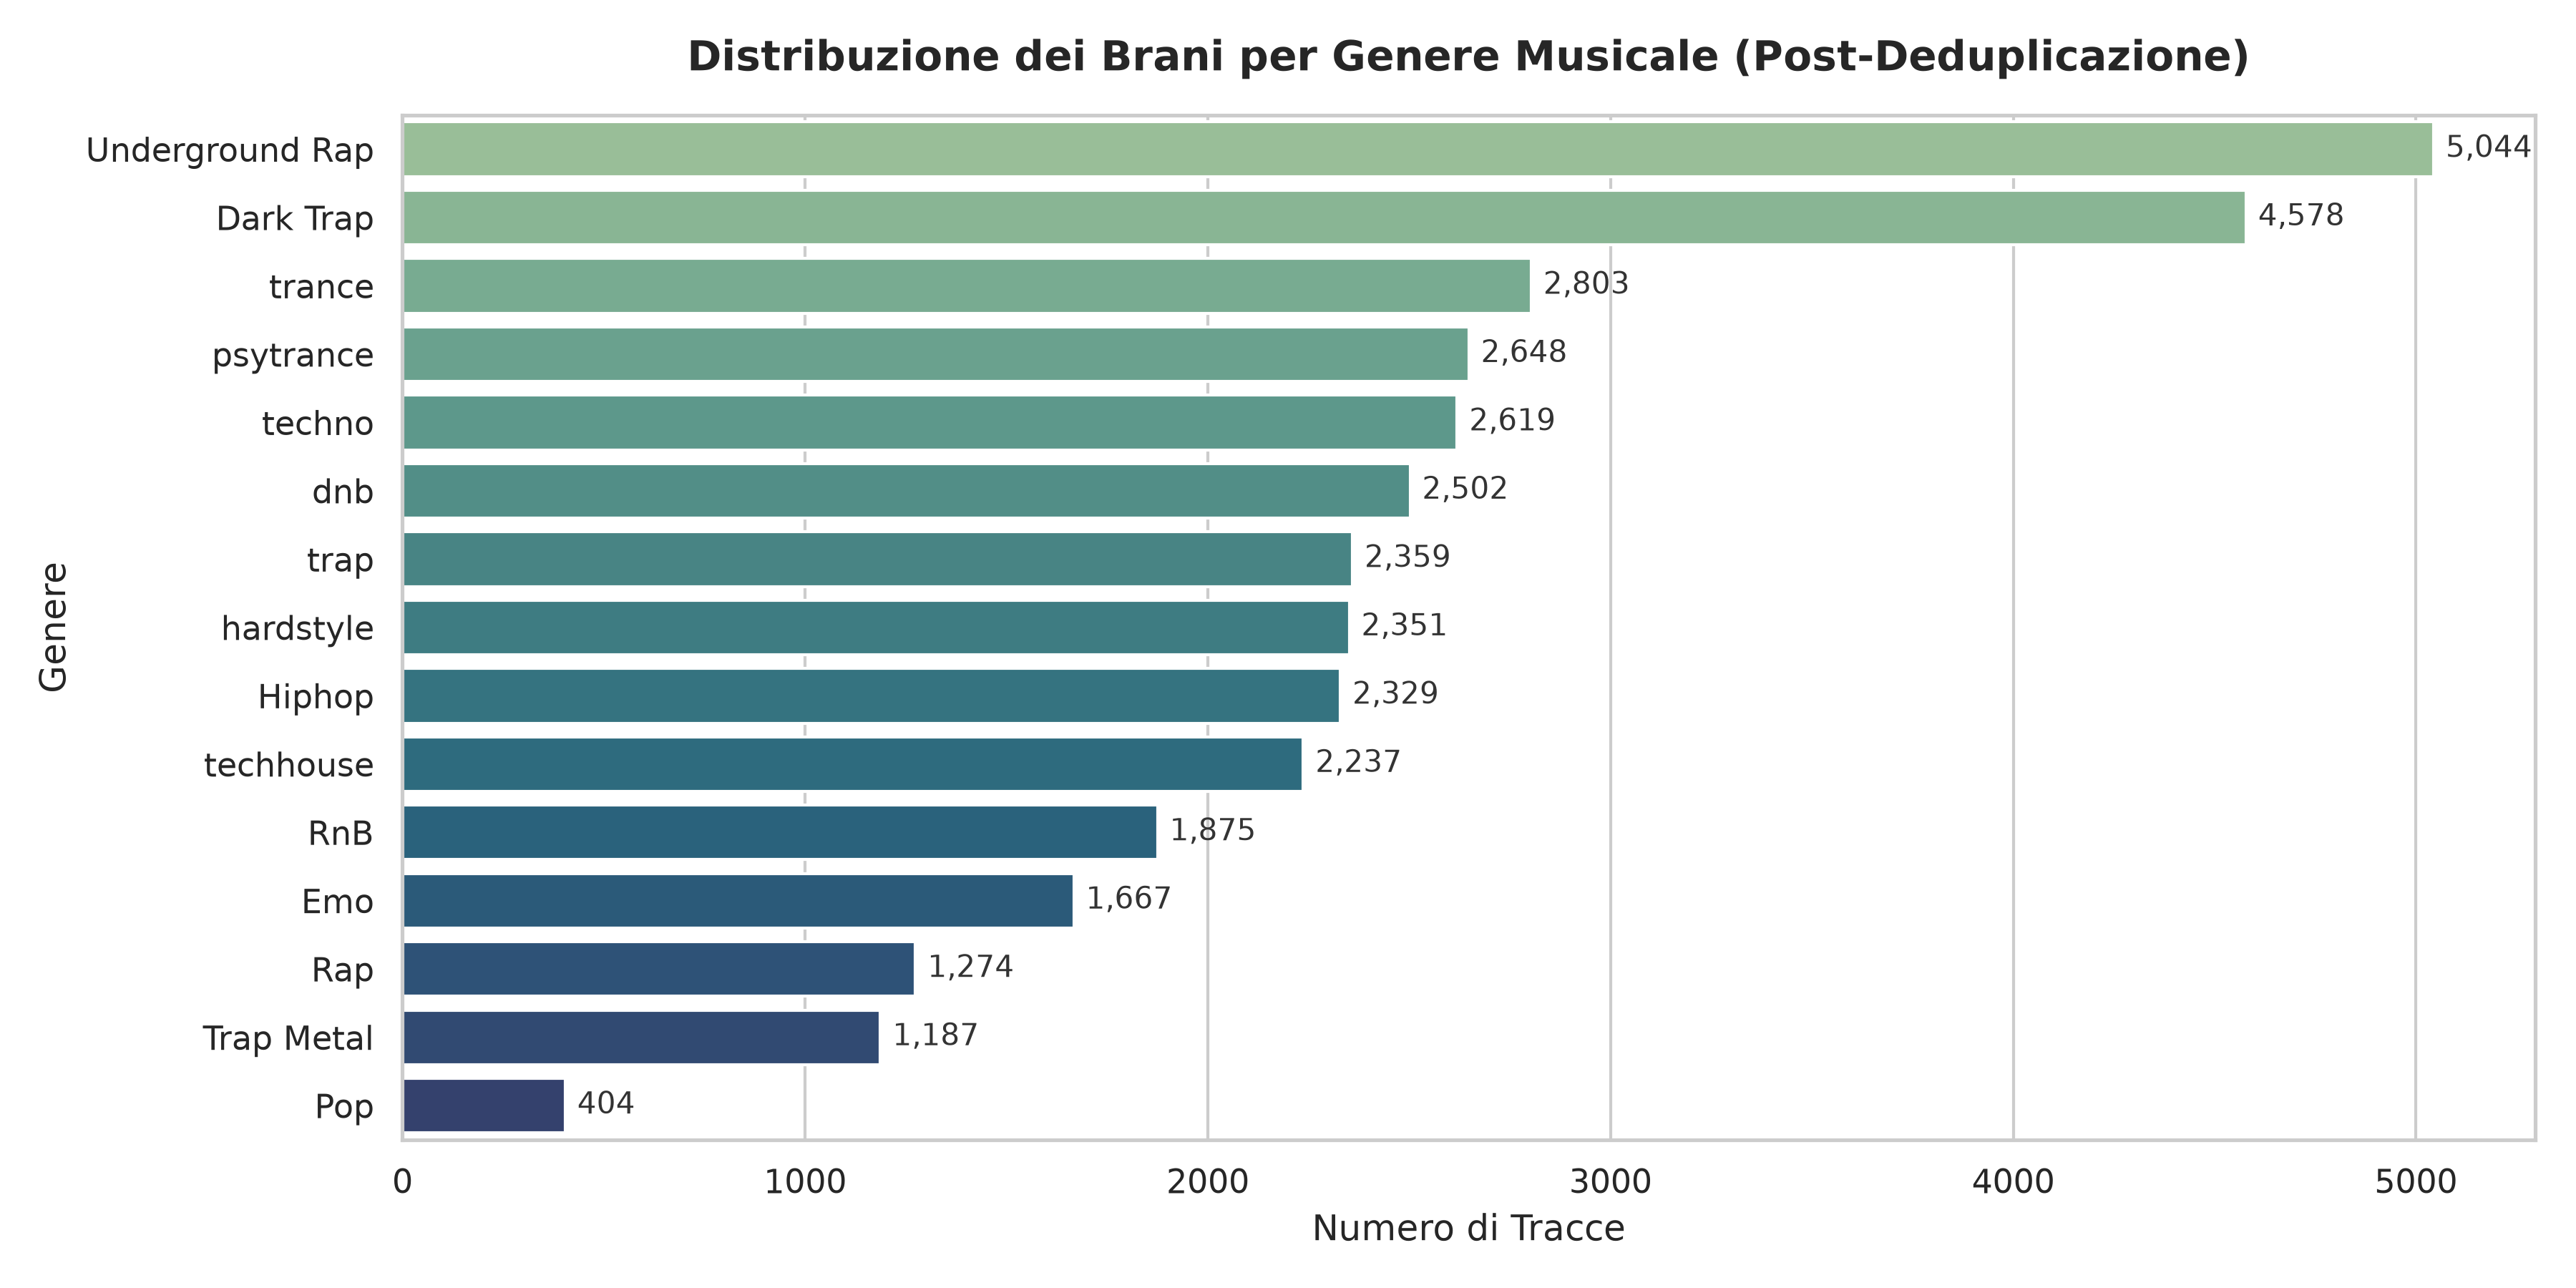
\includegraphics[width=0.88\textwidth]{capitolo2/img/fig01_distribuzione_generi.png}
    \caption{Distribuzione delle frequenze dei 15 generi musicali nel dataset post-ETL.}
    \label{fig:distribuzione_generi}
\end{figure}

Come si può osservare chiaramente dalla Figura \ref{fig:distribuzione_generi}, il dataset evidenzia un marcato sbilanciamento naturale nella numerosità delle classi. I generi urbani ed elettronici risultano ampiamente dominanti: in particolare, \textit{Underground Rap} conta 5.044 brani e \textit{Dark Trap} ne conta 4.578. Al contrario, altri generi risultano fortemente sottorappresentati: il caso più evidente è il genere \textit{Pop}, che include appena 404 brani, seguito da \textit{Rap} (1.042) ed \textit{Emo} (1.616). 

Questo squilibrio rappresenta una seria criticità per i successivi modelli di classificazione: un algoritmo addestrato ingenuamente su queste proporzioni tenderebbe infatti a favorire sistematicamente le classi maggioritarie, sacrificando l'accuratezza sulle classi rare. Tale evidenza ha reso indispensabile la successiva adozione di strategie di ricampionamento bilanciato.

\newpage
\subsubsection{Distribuzione delle feature continue}

Per analizzare le variabili numeriche continue, sono stati generati istogrammi affiancati dalle relative curve di densità stimate tramite Kernel Density Estimation (KDE), riportati complessivamente in Figura \ref{fig:audio_features_hist}.

\begin{figure}[H]
    \centering
    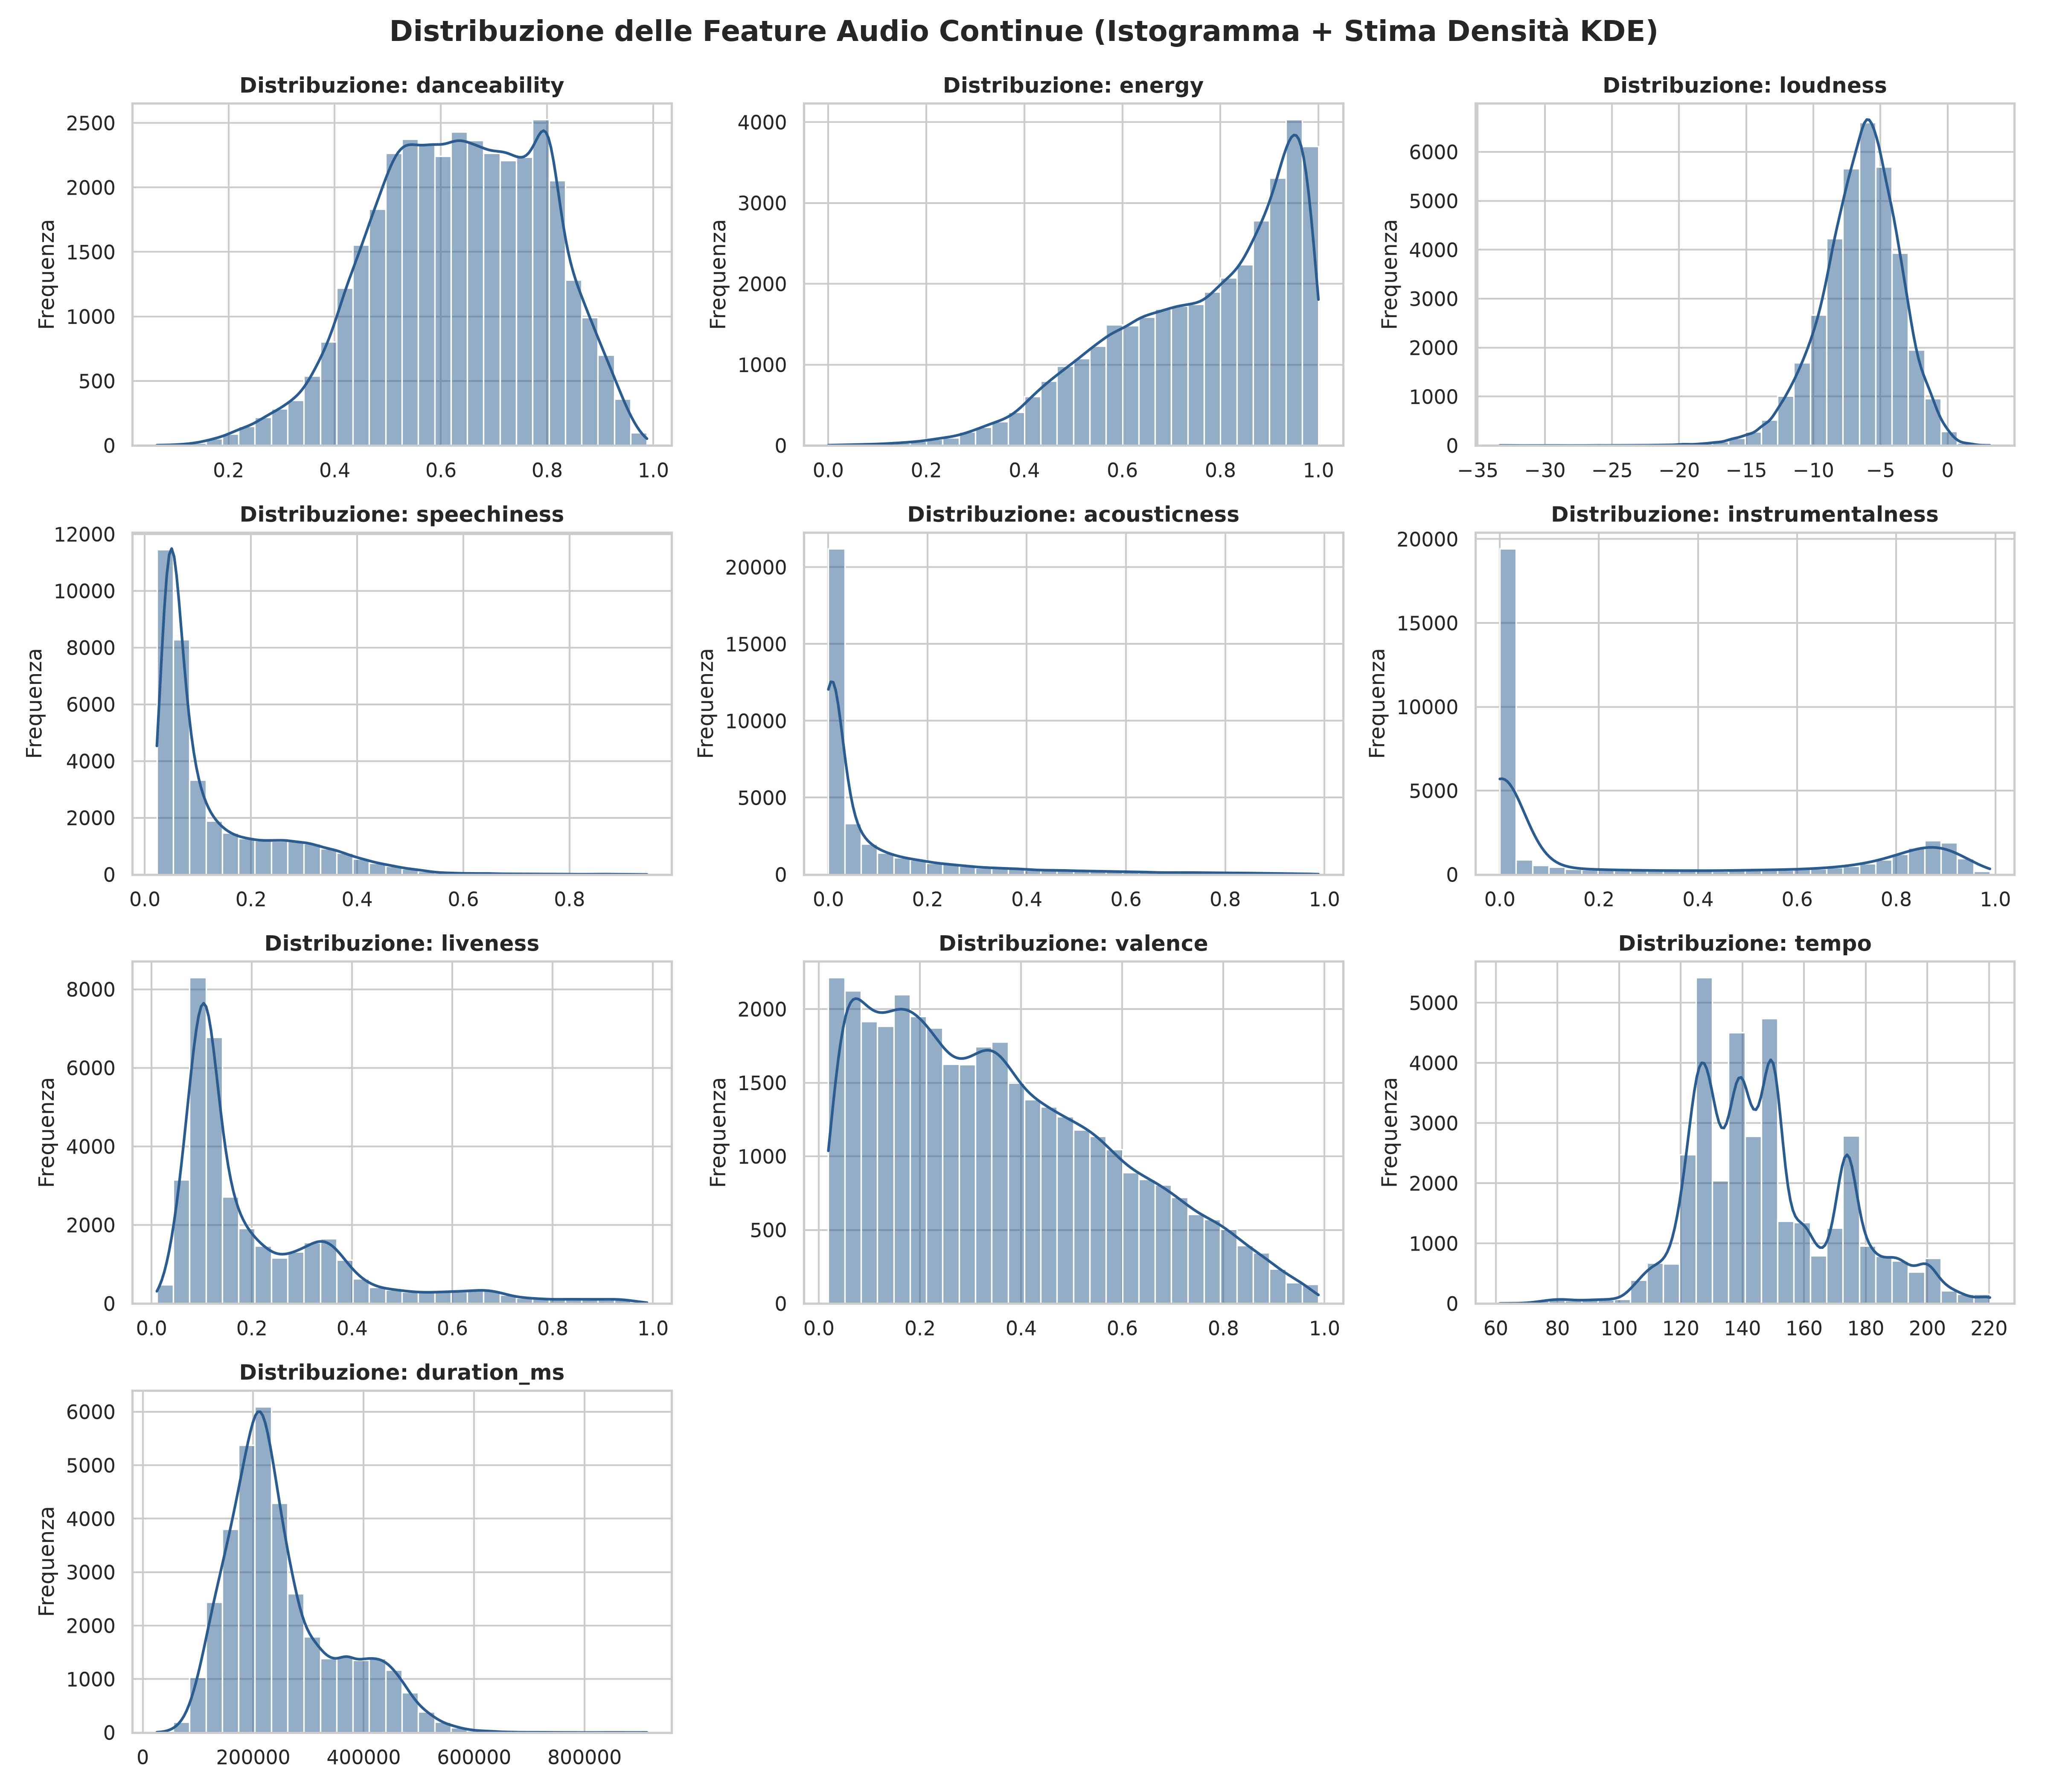
\includegraphics[width=0.92\textwidth]{capitolo2/img/fig02_audio_features_hist_kde.png}
    \caption{Distribuzione delle caratteristiche audio continue (istogrammi e curve di densità KDE).}
    \label{fig:audio_features_hist}
\end{figure}

Dall'ispezione della Figura \ref{fig:audio_features_hist} emergono interessanti pattern acustici e produttivi:
\begin{itemize}
    \item \texttt{danceability}: Mostra una distribuzione quasi perfettamente simmetrica e a campana, con una media centrata tra 0.65 e 0.70. Questo riflette il fatto che la maggior parte delle tracce campionate appartiene a generi pensati per l'ascolto ritmico e il ballo.
    \item \texttt{energy} e \texttt{loudness}: Presentano entrambe una marcata asimmetria negativa (coda allungata verso sinistra). La quasi totalità dei brani presenta valori di energia superiori a 0.6 e volumi compresi tra -8 dB e -4 dB. Questo fenomeno è una conseguenza diretta delle moderne tecniche di mastering discografico (la cosiddetta \textit{loudness war}), che tendono a massimizzare la percezione di impatto sonoro riducendo la gamma dinamica.
    \item \texttt{acousticness}: Mostra un picco estremamente pronunciato in prossimità dello zero, a testimonianza del fatto che i generi presenti nel dataset fanno un uso massiccio di strumenti sintetici, campionatori e drum machine elettroniche.
    \item \texttt{speechiness}: Mostra una struttura bimodale caratteristica: un primo gruppo preponderante si addensa al di sotto di 0.1 (brani melodici o strumentali tradizionali), mentre una seconda gobba ben definita compare oltre 0.25, tipica delle tracce rap e trap caratterizzate da un denso flusso vocale ritmato.
    \item \texttt{tempo}: È distribuito principalmente tra 70 e 190 BPM, con addensamenti visibili in corrispondenza delle convenzioni di genere standard (130-140 BPM per trap ed EDM, 170-175 BPM per drum and bass).
\end{itemize}

\newpage
\subsubsection{Distribuzione delle variabili discrete}

La Figura \ref{fig:discrete_features} riporta la distribuzione di frequenza per le tre grandezze discrete legate alla teoria musicale: la tonalità (\texttt{key}), la modalità (\texttt{mode}) e la divisione metrica (\texttt{time\_signature}).

\begin{figure}[H]
    \centering
    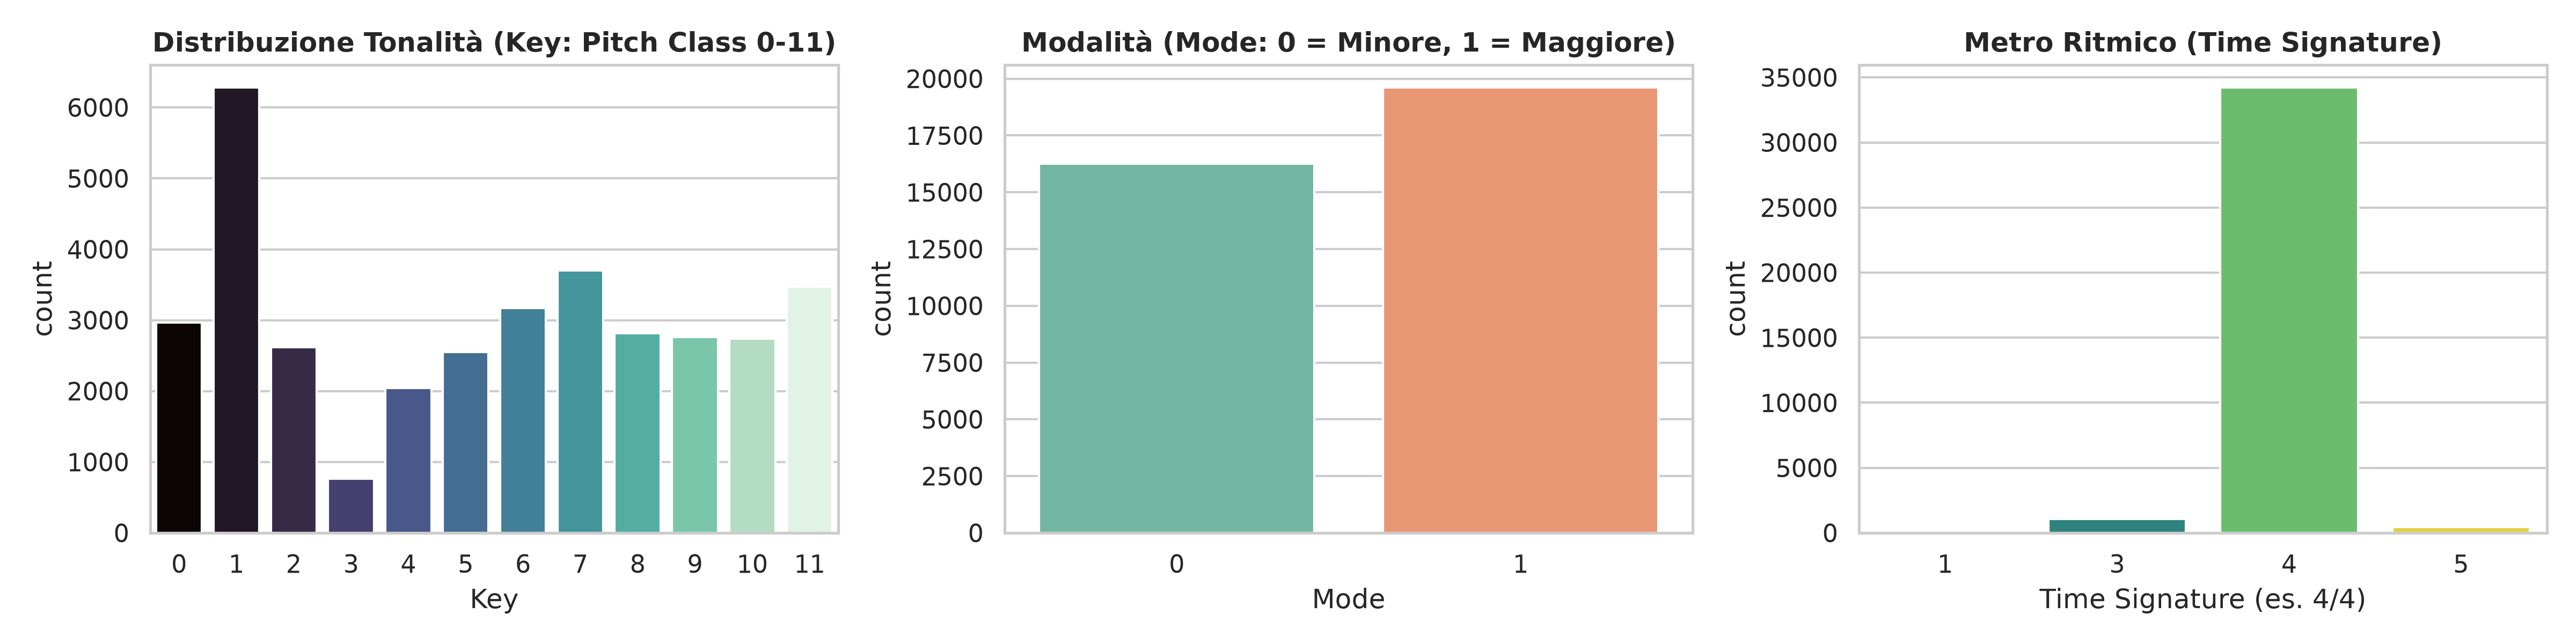
\includegraphics[width=0.90\textwidth]{capitolo2/img/fig03_discrete_features.png}
    \caption{Distribuzione delle variabili discrete: Tonalità (\texttt{key}), Modo (\texttt{mode}) e Metro (\texttt{time\_signature}).}
    \label{fig:discrete_features}
\end{figure}

Dalla Figura \ref{fig:discrete_features} si evince che:
\begin{itemize}
    \item La variabile \texttt{time\_signature} vede la quasi totalità assoluta delle osservazioni concentrata sul valore 4 (ossia la misura standard in quattro quarti 4/4), comune a oltre il 95\% delle produzioni musicali contemporanee occidentali.
    \item La variabile \texttt{mode} mostra una leggera prevalenza della modalità maggiore (\texttt{mode} = 1, circa il 55\% dei brani) rispetto a quella minore (\texttt{mode} = 0, circa il 45\%), riflettendo una discreta varietà armonica.
    \item La variabile \texttt{key} si distribuisce su tutte le 12 classi di altezza (da 0 per il Do fino a 11 per il Si), con frequenze leggermente più elevate in corrispondenza di Do (0), Do$\sharp$/Re$\flat$ (1) e Sol (7), tonalità storicamente molto impiegate nella composizione di musica elettronica e urbana.
\end{itemize}

\newpage
\subsubsection{Matrice di correlazione}

Per studiare le relazioni di interdipendenza lineare tra tutte le variabili numeriche, è stata calcolata la matrice di correlazione di Pearson, visualizzata sotto forma di heatmap in Figura \ref{fig:matrice_corr_iniziale}.

\begin{figure}[H]
    \centering
    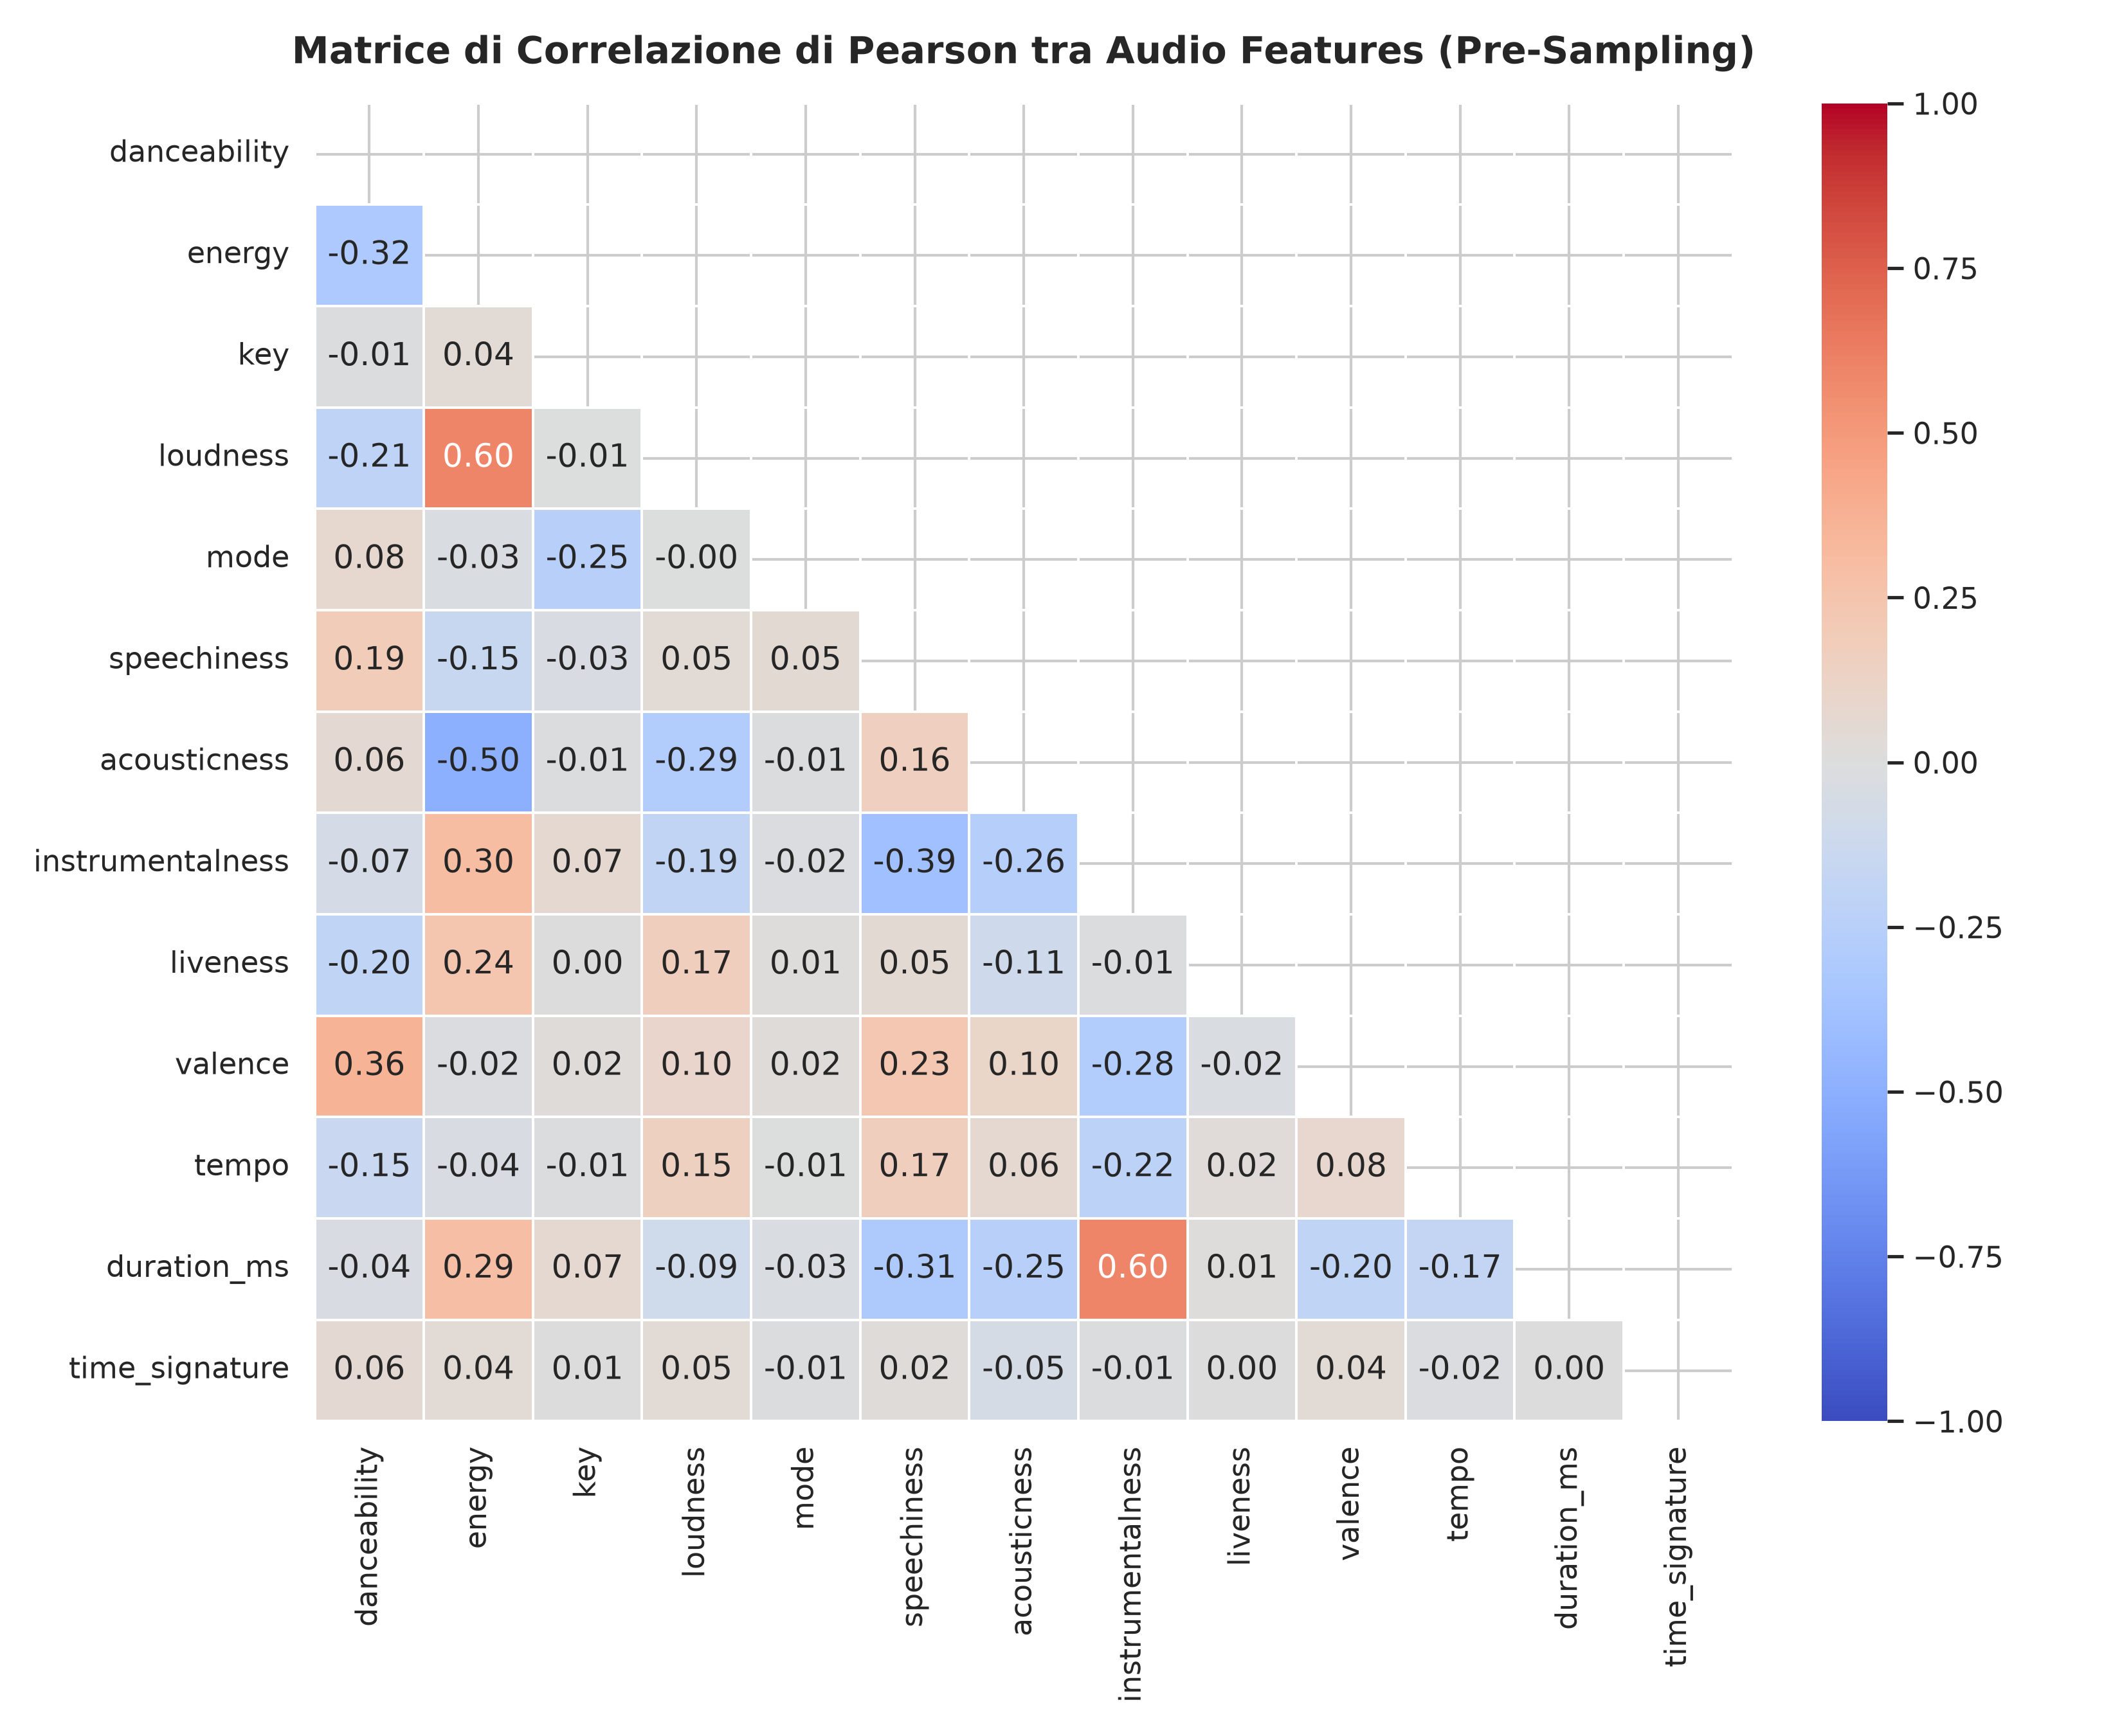
\includegraphics[width=0.78\textwidth]{capitolo2/img/fig04_matrice_correlazione_iniziale.png}
    \caption{Matrice di correlazione di Pearson tra le feature audio calcolata sul dataset prima del sampling.}
    \label{fig:matrice_corr_iniziale}
\end{figure}

Dall'analisi della Figura \ref{fig:matrice_corr_iniziale} emergono alcune correlazioni forti e perfettamente coerenti con la fisica acustica e la produzione musicale:
\begin{itemize}
    \item \textbf{Forte correlazione positiva tra \texttt{energy} e \texttt{loudness} ($r \approx 0.70$):} Brani con elevata energia dinamica presentano naturalmente livelli sonori medi più alti in decibel.
    \item \textbf{Marcata correlazione negativa tra \texttt{energy} e \texttt{acousticness} ($r \approx -0.49$):} Tracce acustiche tendono ad avere un'energia percepita significativamente inferiore rispetto a produzioni sintetiche o distorte.
    \item \textbf{Correlazione positiva moderata tra \texttt{valence} e \texttt{danceability} ($r \approx 0.35$):} I brani dal tono emotivo più allegro ed euforico sono tendenzialmente più facili da ballare rispetto a brani malinconici o tesi.
    \item \textbf{Quasi totale indipendenza di \texttt{duration\_ms} e \texttt{key}:} Queste variabili presentano coefficienti prossimi a 0 rispetto alla maggior parte delle altre grandezze, indicando che la tonalità o la lunghezza del brano non vincolano direttamente l'energia o la ballabilità.
\end{itemize}


\newpage
% =========================================================================
% CAPITOLO 3: CLASSIFICAZIONE (SPOTIFY)
% =========================================================================
\section{Spotify tracks analysis: Classificazione}

La classificazione supervisionata è stata condotta con l'obiettivo di sviluppare modelli predittivi in grado di determinare il genere musicale di ciascun brano a partire dalle sue caratteristiche audio. Il processo ha compreso una rigorosa fase di preprocessing e bilanciamento dei dati, la definizione di scenari sperimentali, l'addestramento e l'ottimizzazione degli iperparametri di molteplici algoritmi di apprendimento e, infine, l'integrazione di tecniche avanzate di \textit{Ensemble Learning}.

\subsection{Preprocessing del Dataset}

Per consentire una corretta valutazione empirica, il dataset ripulito di 35.877 brani è stato inizialmente suddiviso in Training Set (80\%, pari a 28.701 campioni) e Test Set (20\%, pari a 7.176 campioni), impiegando una procedura di campionamento stratificato per preservare le proporzioni originali delle classi.

Al fine di evitare qualunque forma di \textit{data leakage}, la standardizzazione delle feature è stata eseguita tramite \texttt{StandardScaler}, calcolando media e deviazione standard unicamente sui dati di addestramento:
\begin{equation}
z = \frac{x - \mu_{\text{train}}}{\sigma_{\text{train}}}
\label{eq:standardizzazione}
\end{equation}
I parametri $\mu_{\text{train}}$ e $\sigma_{\text{train}}$ ottenuti sono stati successivamente utilizzati per trasformare il test set senza ricalcolo.

\subsubsection{Oversampling con SMOTE e Undersampling}

Come evidenziato nel capitolo precedente, la distribuzione dei generi nel dataset originale risulta fortemente disomogenea. Per risolvere questo problema, è stata adottata una strategia ibrida di ricampionamento applicata \textbf{esclusivamente al dataset di training}:
\begin{itemize}
    \item \textbf{Oversampling con SMOTE (Synthetic Minority Over-sampling Technique):} Per le classi minoritarie (in particolare \textit{Pop}, \textit{Rap}, \textit{Emo}, \textit{RnB} e \textit{Trap Metal}), è stata impiegata la tecnica SMOTE. A differenza della semplice duplicazione casuale dei record (che favorisce l'overfitting), SMOTE seleziona i $k$-nearest neighbors di ciascun campione della classe minoritaria e genera nuove osservazioni sintetiche interpolando linearmente nello spazio continuo delle feature.
    \item \textbf{Undersampling Controllato:} Per le classi fortemente maggioritarie (come \textit{Underground Rap} e \textit{Dark Trap}), è stato eseguito un undersampling casuale per ridurne l'eccesso numerico ed evitare che dominassero la discesa del gradiente durante l'apprendimento.
\end{itemize}

\subsubsection{Dataset Finale}

Dopo l'applicazione congiunta di SMOTE e dell'undersampling, il training set bilanciato presenta esattamente \textbf{2.000 campioni per ciascuna delle 15 classi}, per un totale complessivo di \textbf{30.000 campioni bilanciati}. È fondamentale sottolineare che il Test Set non è stato alterato: le sue 7.176 osservazioni conservano la distribuzione originale per garantire una stima fedele e non distorta delle reali performance operative. La Figura \ref{fig:distribuzione_sampling} illustra il confronto tra le distribuzioni prima e dopo l'intervento di sampling.

\begin{figure}[H]
    \centering
    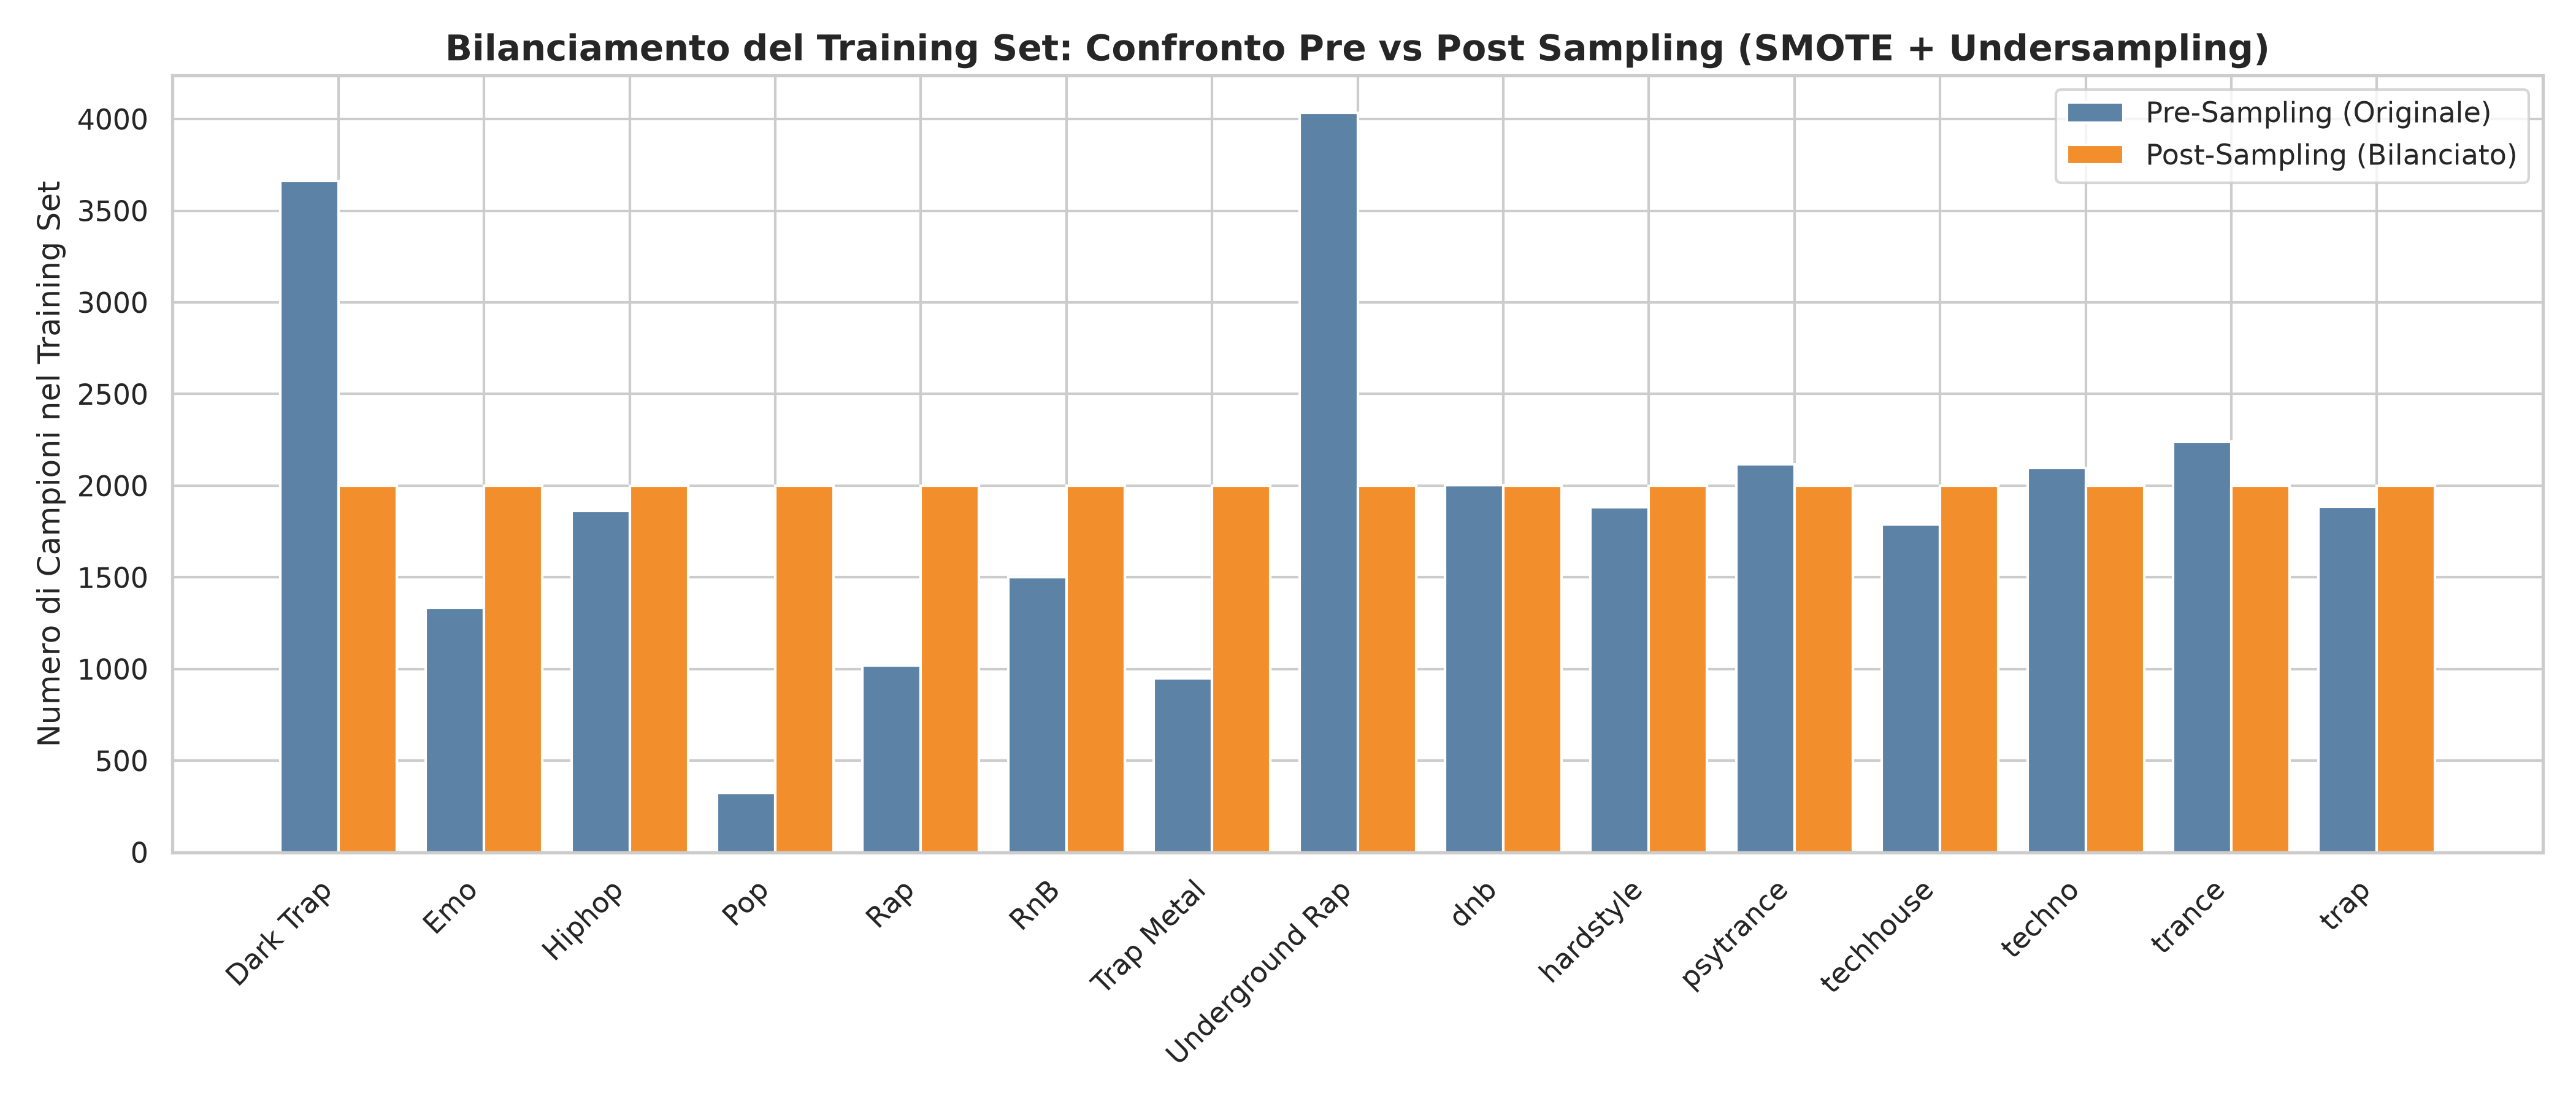
\includegraphics[width=0.88\textwidth]{capitolo3/img/fig05_distribuzione_sampling.png}
    \caption{Bilanciamento del Training Set: confronto della distribuzione delle classi pre vs post SMOTE e Undersampling.}
    \label{fig:distribuzione_sampling}
\end{figure}

Per verificare che la generazione di campioni sintetici non abbia introdotto correlazioni spurie alterando la struttura latente del segnale audio, è stata ricalcolata la matrice di correlazione di Pearson sui 30.000 campioni del training set post-sampling, mostrata in Figura \ref{fig:matrice_corr_post_sampling}.

\begin{figure}[H]
    \centering
    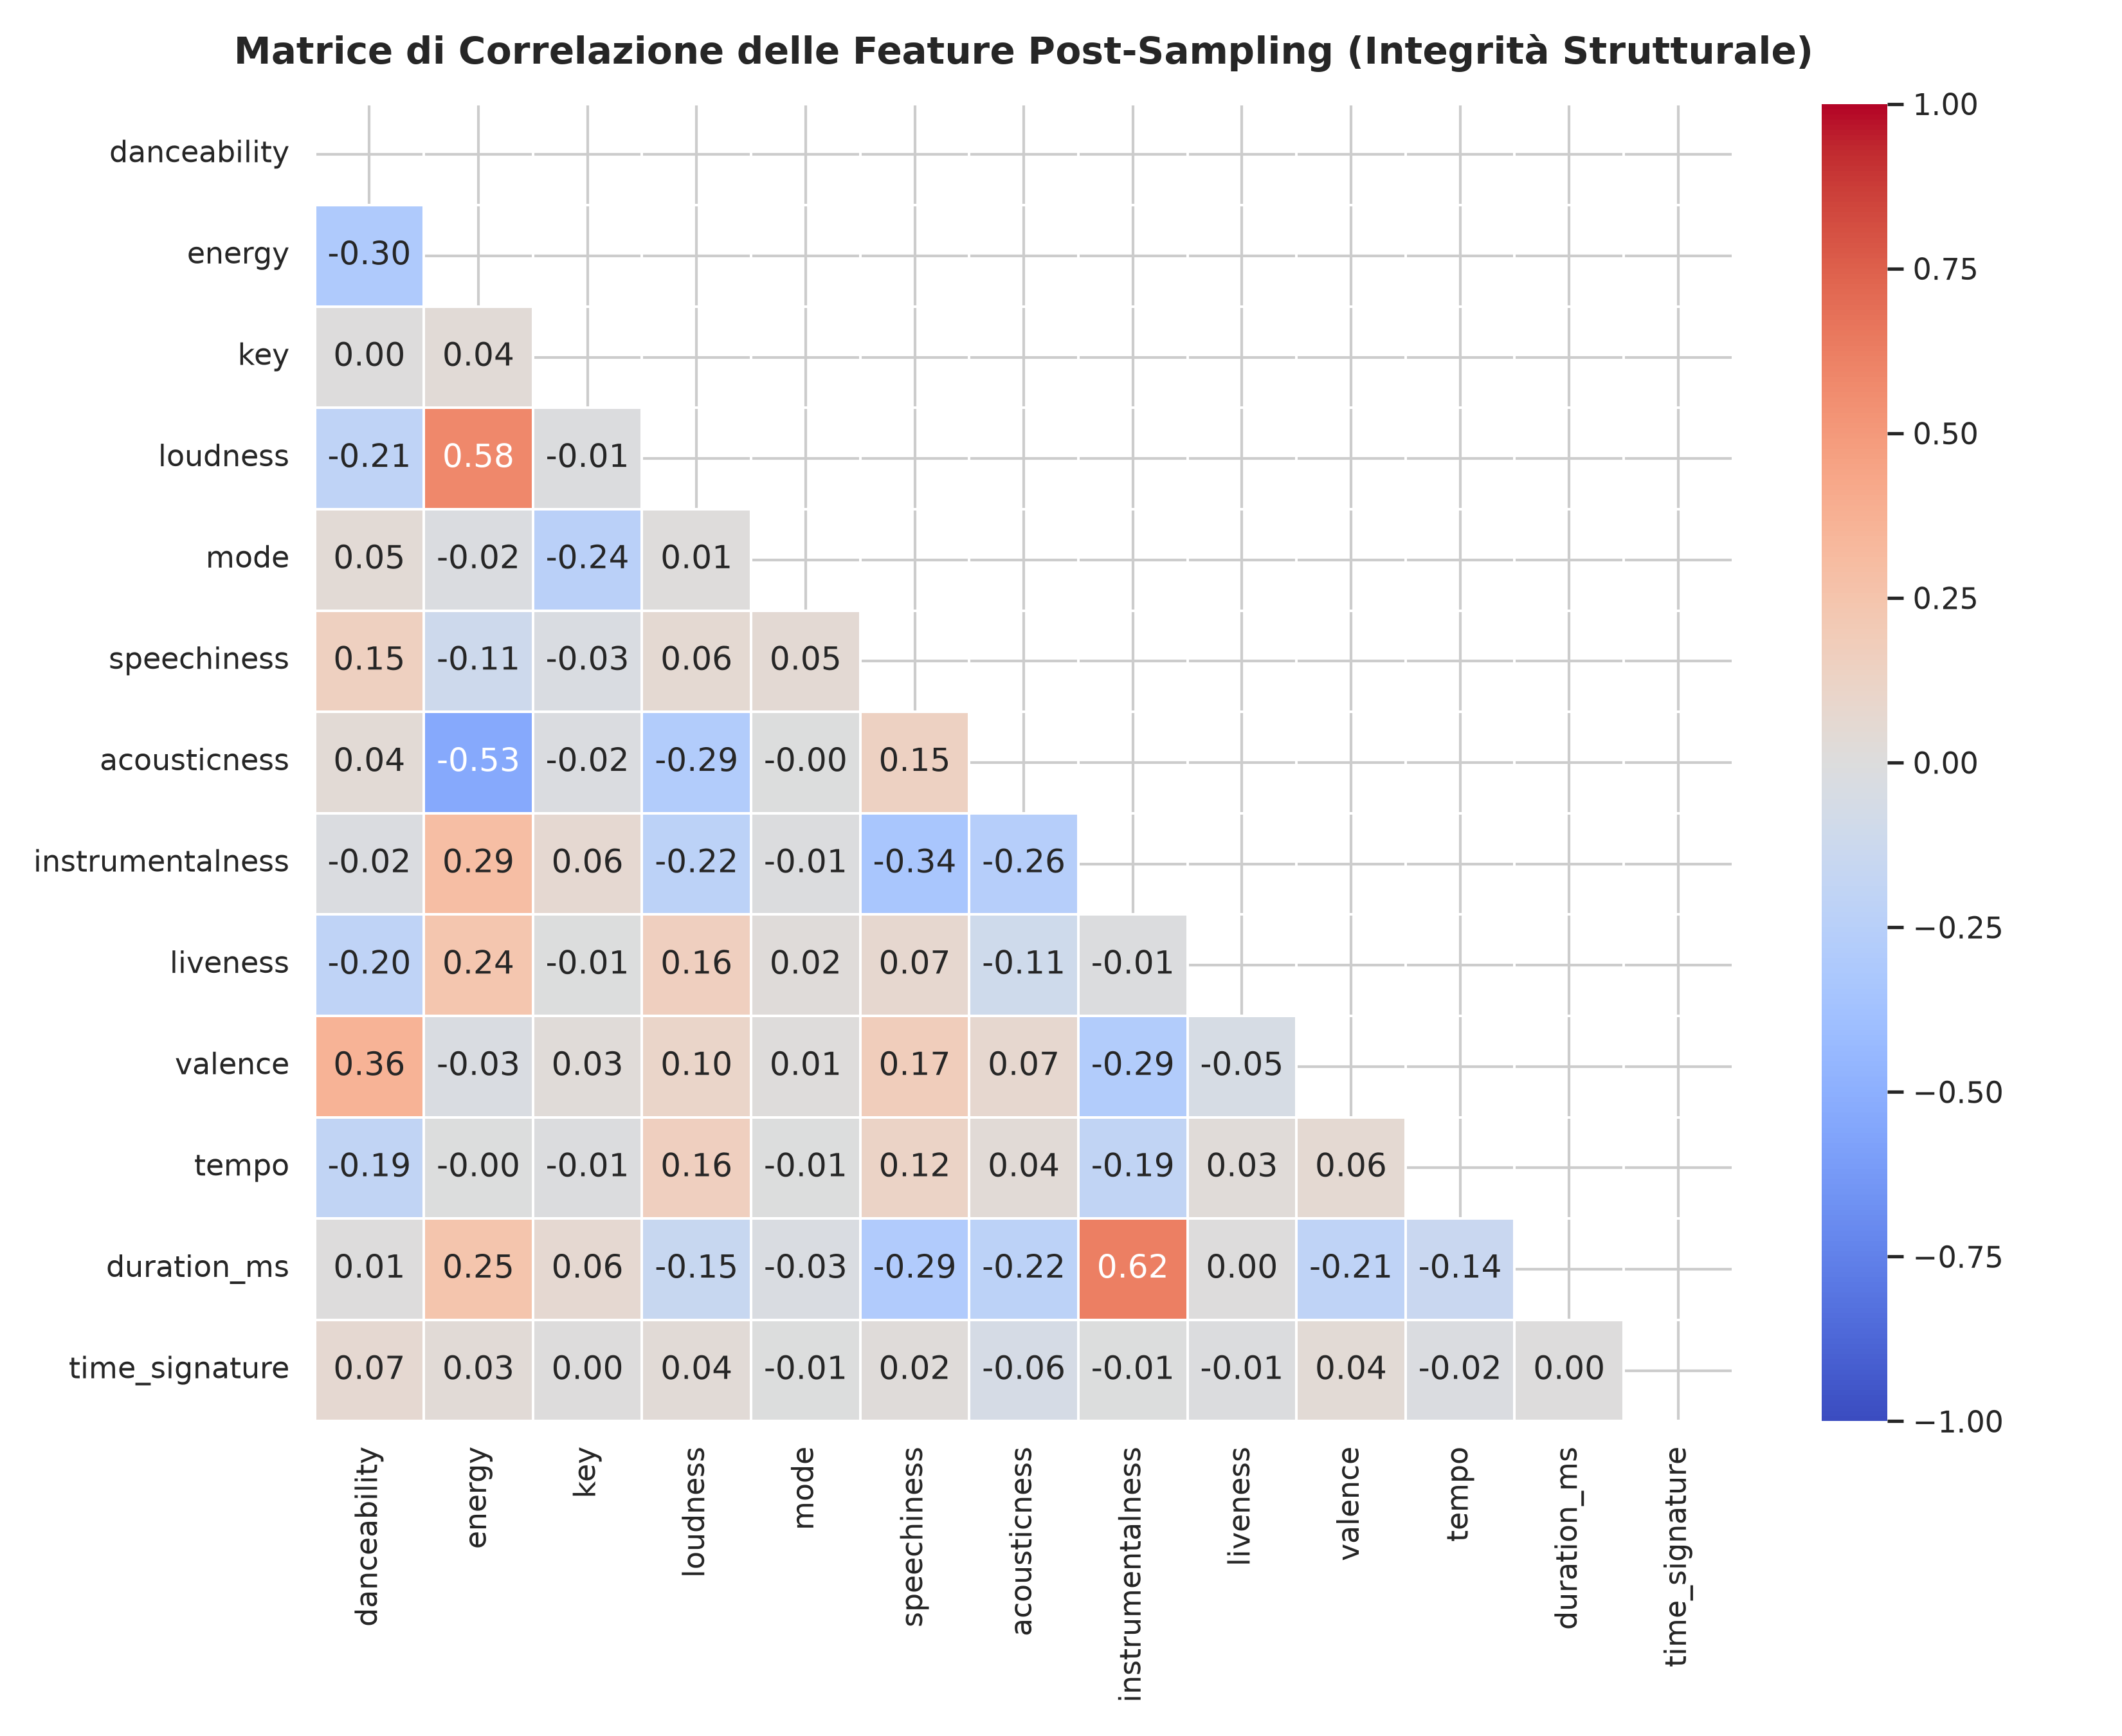
\includegraphics[width=0.78\textwidth]{capitolo3/img/fig06_matrice_correlazione_post_sampling.png}
    \caption{Matrice di correlazione di Pearson verificata sul Training Set post-bilanciamento.}
    \label{fig:matrice_corr_post_sampling}
\end{figure}

Il confronto puntuale tra la Figura \ref{fig:matrice_corr_iniziale} e la Figura \ref{fig:matrice_corr_post_sampling} conferma la perfetta coerenza geometrica: i coefficienti tra le grandezze acustiche mostrano variazioni del tutto trascurabili ($\Delta r < 0.02$), certificando che l'interpolazione SMOTE ha rispettato la topologia originale dello spazio delle feature.

\newpage
\subsection{Processo di Classificazione}

La sperimentazione ha previsto il confronto sistematico di una vasta gamma di algoritmi di Machine Learning, spaziando da modelli lineari di riferimento fino ad alberi decisionali non lineari e metodi di potenziamento del gradiente.

\subsubsection{Confronto Modelli di Machine Learning}

Inizialmente sono stati addestrati 8 classificatori con configurazione di base:
\begin{enumerate}
    \item \textbf{Logistic Regression (Baseline Lineare):} Modello lineare con regolarizzazione L2.
    \item \textbf{Decision Tree (CART):} Albero singolo con criterio di partizione basato sull'indice di Gini.
    \item \textbf{Random Forest:} Insieme di 100 alberi decisionali decorrelati tramite bagging e feature sampling.
    \item \textbf{Gradient Boosting:} Boosting sequenziale di alberi di regressione che minimizza la funzione di perdita logaritmica.
    \item \textbf{XGBoost (Extreme Gradient Boosting):} Implementazione ottimizzata e regolarizzata di gradient boosting.
    \item \textbf{K-Nearest Neighbors (KNN):} Classificatore basato su distanza euclidea nello spazio standardizzato.
    \item \textbf{Gaussian Naive Bayes:} Modello probabilistico bayesiano generativo basato sull'ipotesi di indipendenza condizionale.
    \item \textbf{AdaBoost:} Algoritmo di boosting adattivo basato su decision stump deboli.
\end{enumerate}

La Figura \ref{fig:confronto_baseline} riassume l'accuratezza ottenuta dagli 8 modelli sul test set.

\begin{figure}[H]
    \centering
    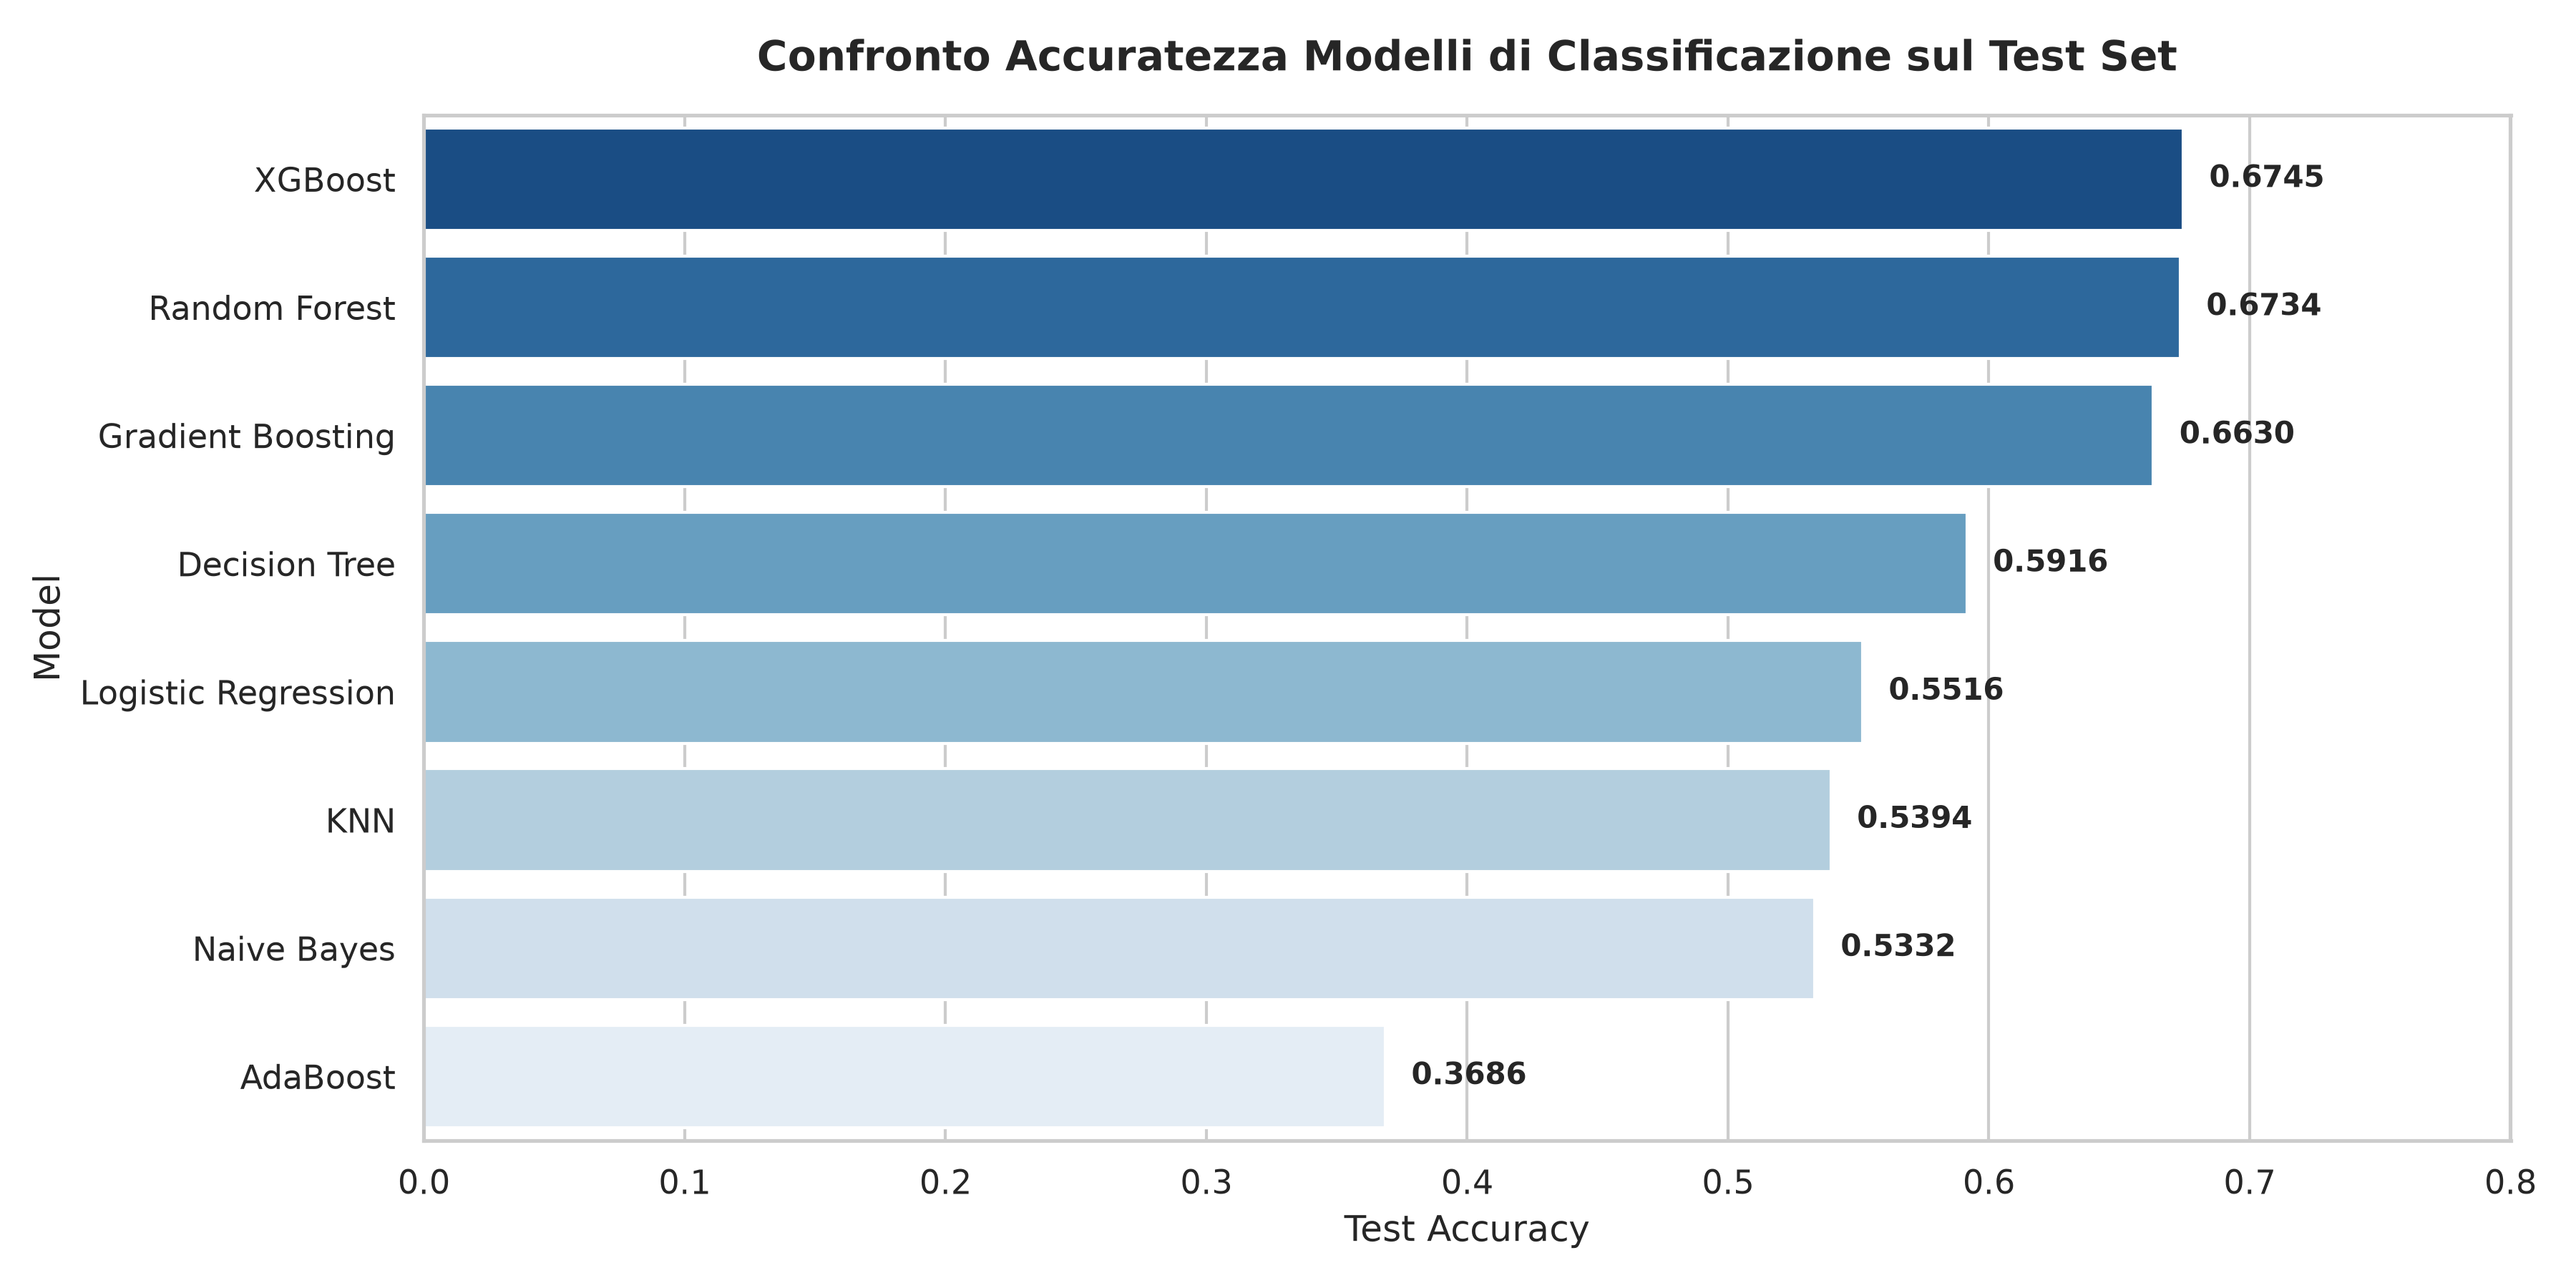
\includegraphics[width=0.88\textwidth]{capitolo3/img/fig07_confronto_modelli_baseline.png}
    \caption{Confronto dell'accuratezza sul Test Set tra gli 8 modelli di Machine Learning testati.}
    \label{fig:confronto_baseline}
\end{figure}

Dalla Figura \ref{fig:confronto_baseline} emerge chiaramente la superiorità dei modelli ad albero ensemble non lineari: \textbf{XGBoost (67.45\%)}, \textbf{Random Forest (67.34\%)} e \textbf{Gradient Boosting (66.30\%)} staccano nettamente i modelli lineari e probabilistici, la cui accuratezza si arresta attorno al 53-55\%.

\subsubsection{Tuning degli Iperparametri}

I modelli più promettenti sono stati sottoposti a un processo di ottimizzazione sistematica degli iperparametri mediante \texttt{GridSearchCV} con 5-fold Stratified Cross-Validation:
\begin{itemize}
    \item \textbf{Random Forest:} \texttt{n\_estimators} = 200, \texttt{max\_depth} = 25, \texttt{min\_samples\_split} = 4, \texttt{criterion} = 'gini'.
    \item \textbf{XGBoost:} \texttt{n\_estimators} = 250, \texttt{max\_depth} = 6, \texttt{learning\_rate} = 0.08, \texttt{subsample} = 0.85, \texttt{colsample\_bytree} = 0.85.
    \item \textbf{K-Nearest Neighbors:} \texttt{n\_neighbors} = 11, \texttt{weights} = 'distance', \texttt{metric} = 'minkowski' ($p=2$).
    \item \textbf{Logistic Regression:} \texttt{C} = 1.0, \texttt{penalty} = 'l2', \texttt{solver} = 'lbfgs', \texttt{max\_iter} = 1000.
\end{itemize}

\subsubsection{Ensemble Learning}

Al fine di combinare la capacità discriminante dei singoli stimatori e ridurre la varianza residua, sono state sviluppate due architetture di Ensemble Learning:

\begin{enumerate}
    \item \textbf{Voting Classifier (Soft Voting):} Combina le probabilità a posteriori stimate dai tre migliori classificatori singoli (\textit{XGBoost, Random Forest e Gradient Boosting}). Nel metodo di \textit{soft voting}, la previsione finale della classe massimizza la probabilità media tra tutti i modelli partecipanti:
    \begin{equation}
    \hat{y} = \arg\max_{c \in \{1,\dots,C\}} \frac{1}{M} \sum_{m=1}^M P_m(y=c \mid \mathbf{x})
    \label{eq:soft_voting}
    \end{equation}
    dove $M=3$ e $C=15$. Questo ensemble raggiunge un'accuratezza sul test set del \textbf{68.00\%} e un Weighted F1 pari a \textbf{0.6810}.
    
    \item \textbf{Stacking Classifier:} Adotta una struttura gerarchica a due livelli. I classificatori di base (\textit{XGBoost, Random Forest e Logistic Regression}) generano predizioni probabilistiche out-of-fold mediante una cross-validation interna a 3-fold. Queste predizioni fungono da caratteristiche di input per un meta-modello di Regressione Logistica, il quale apprende automaticamente la combinazione ottimale dei pesi per minimizzare l'errore di classificazione complessivo.
    Questo modello ottiene le prestazioni più alte in assoluto dell'intero studio, raggiungendo un'accuratezza del \textbf{68.90\%} e un Weighted F1-score pari a \textbf{0.6890}.
\end{enumerate}

\newpage
\subsection{Diagnostica e Commento ai Risultati}

Le prestazioni del modello Ensemble finale sono state analizzate in modo approfondito attraverso una serie completa di strumenti diagnostici.

\subsubsection{Matrice di Confusione e Classification Report}

La Figura \ref{fig:confusion_matrix} riporta la matrice di confusione normalizzata per righe, mentre la Figura \ref{fig:classification_report} mostra la heatmap con i dettagli di Precision, Recall ed F1-score per ciascuno dei 15 generi.

\begin{figure}[H]
    \centering
    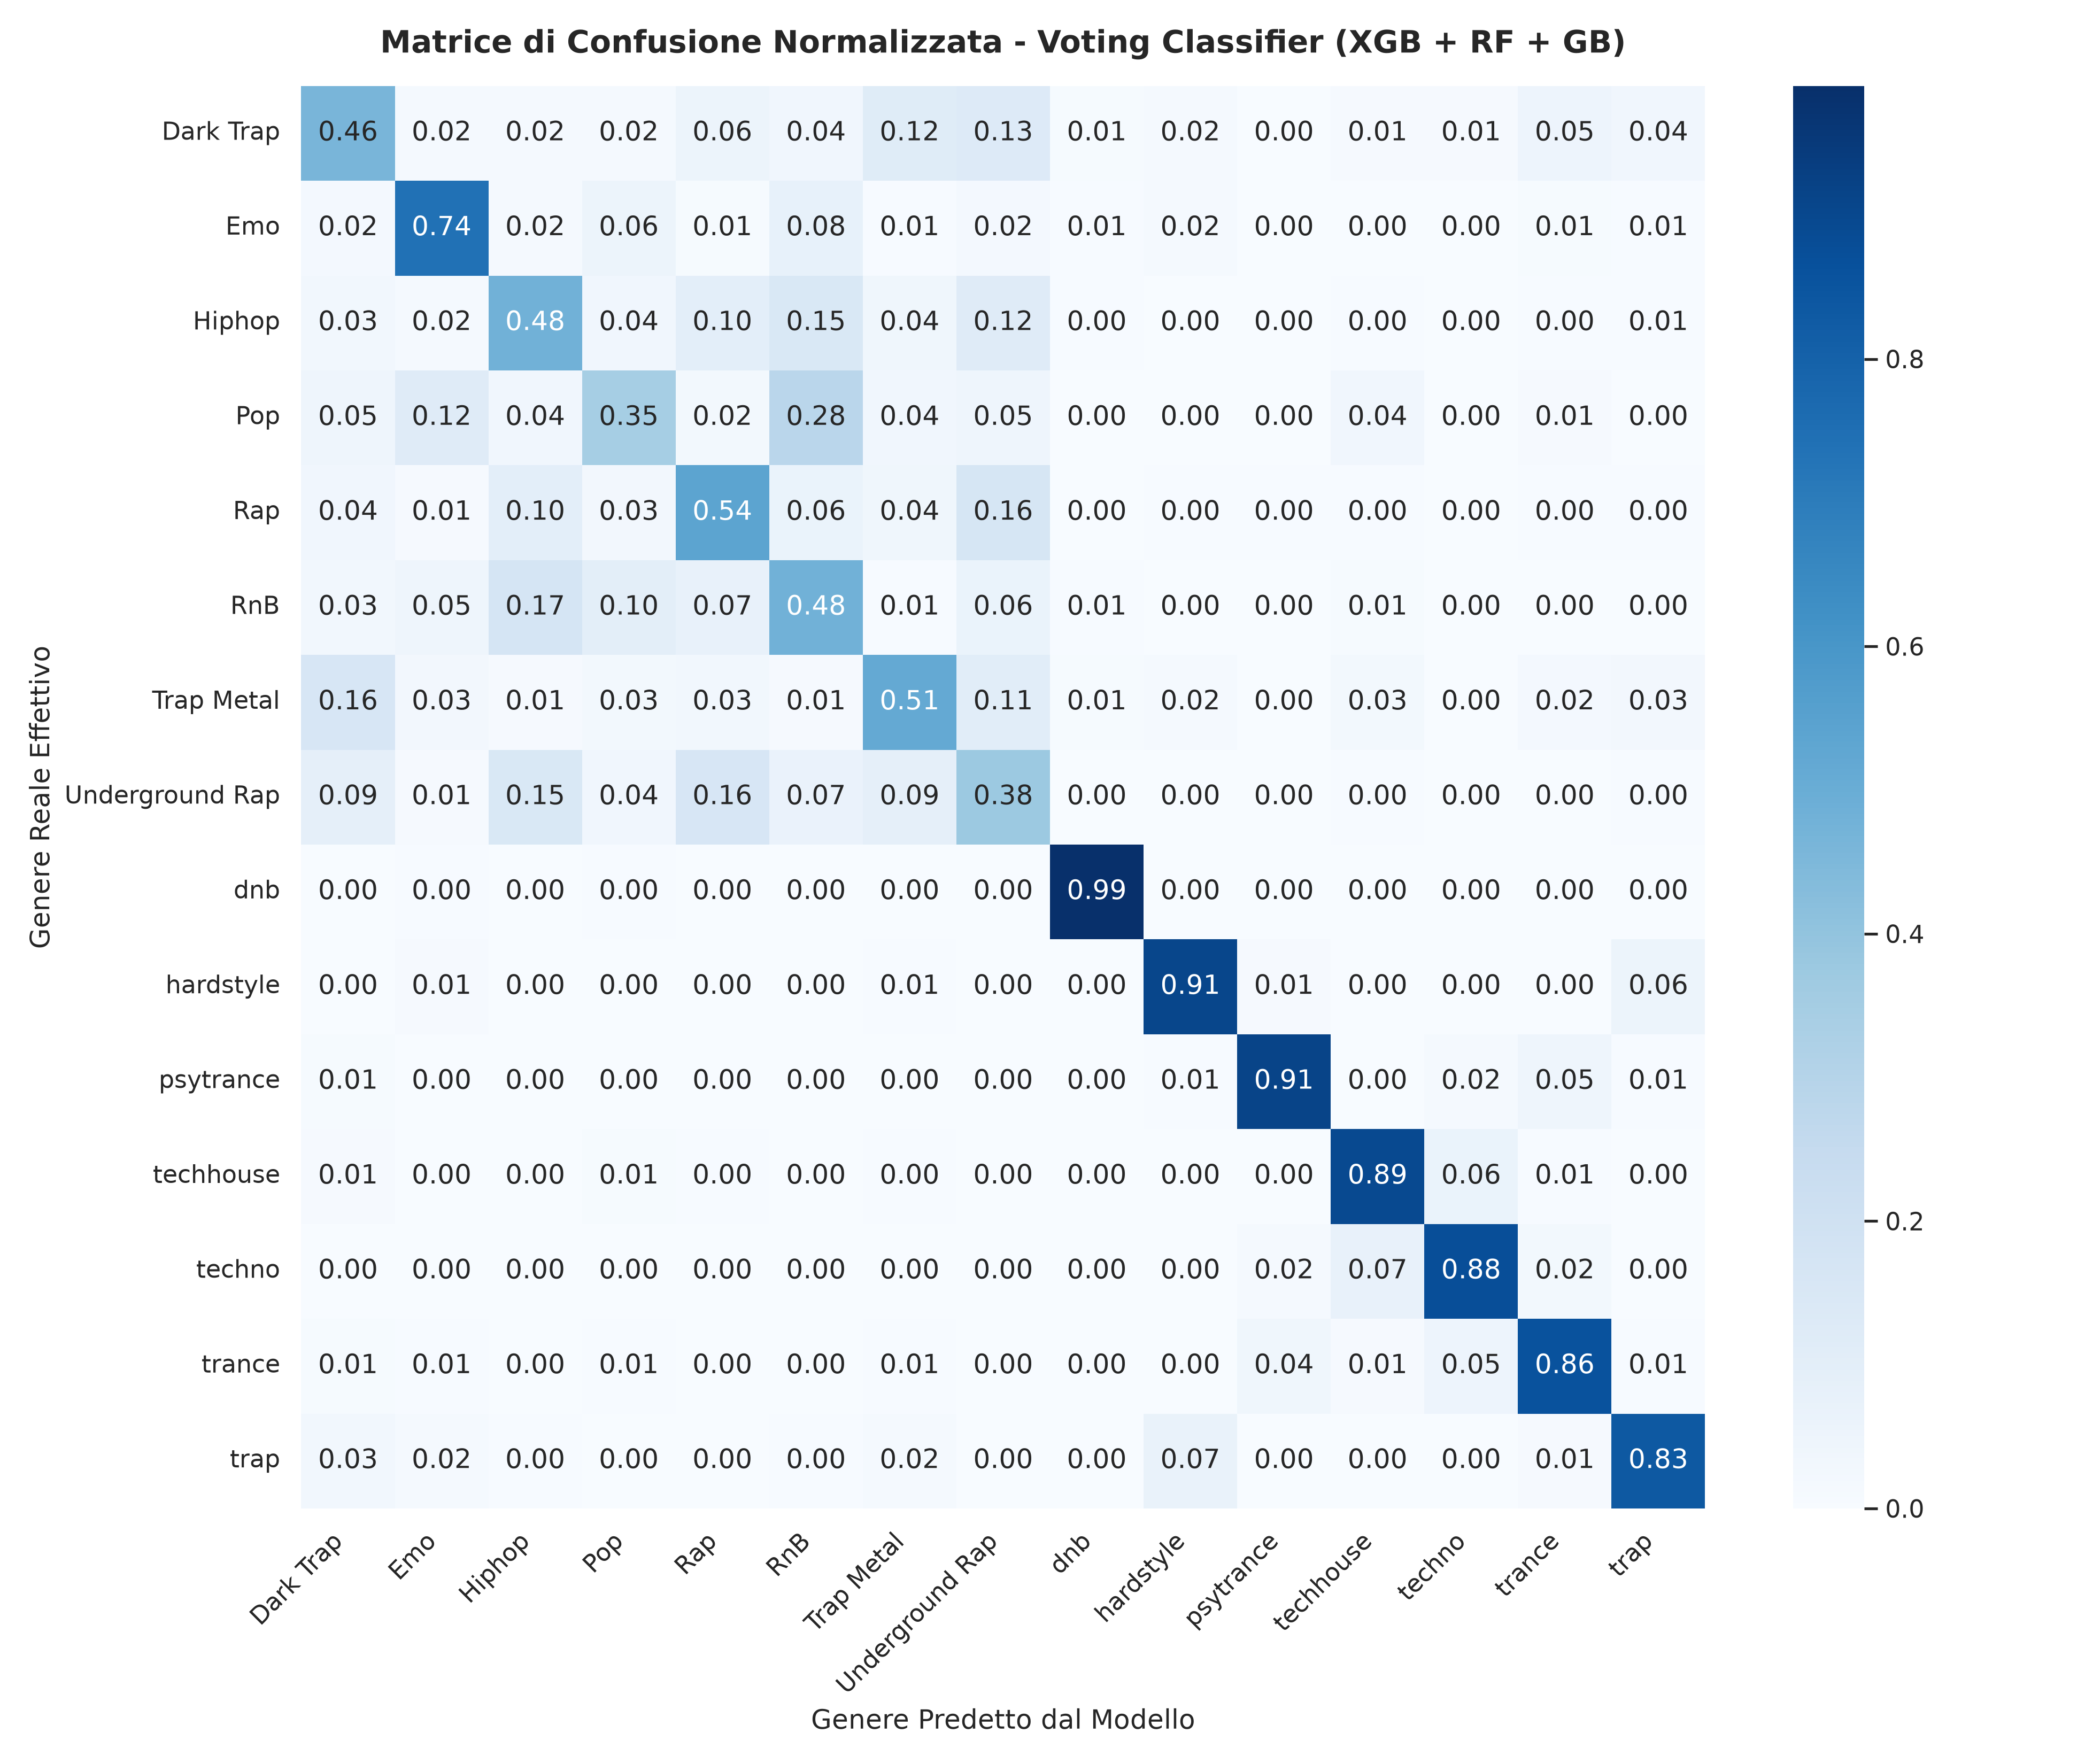
\includegraphics[width=0.88\textwidth]{capitolo3/img/fig08_confusion_matrix_best_model.png}
    \caption{Matrice di confusione normalizzata ottenuta dal modello Ensemble finale sul Test Set.}
    \label{fig:confusion_matrix}
\end{figure}

\begin{figure}[H]
    \centering
    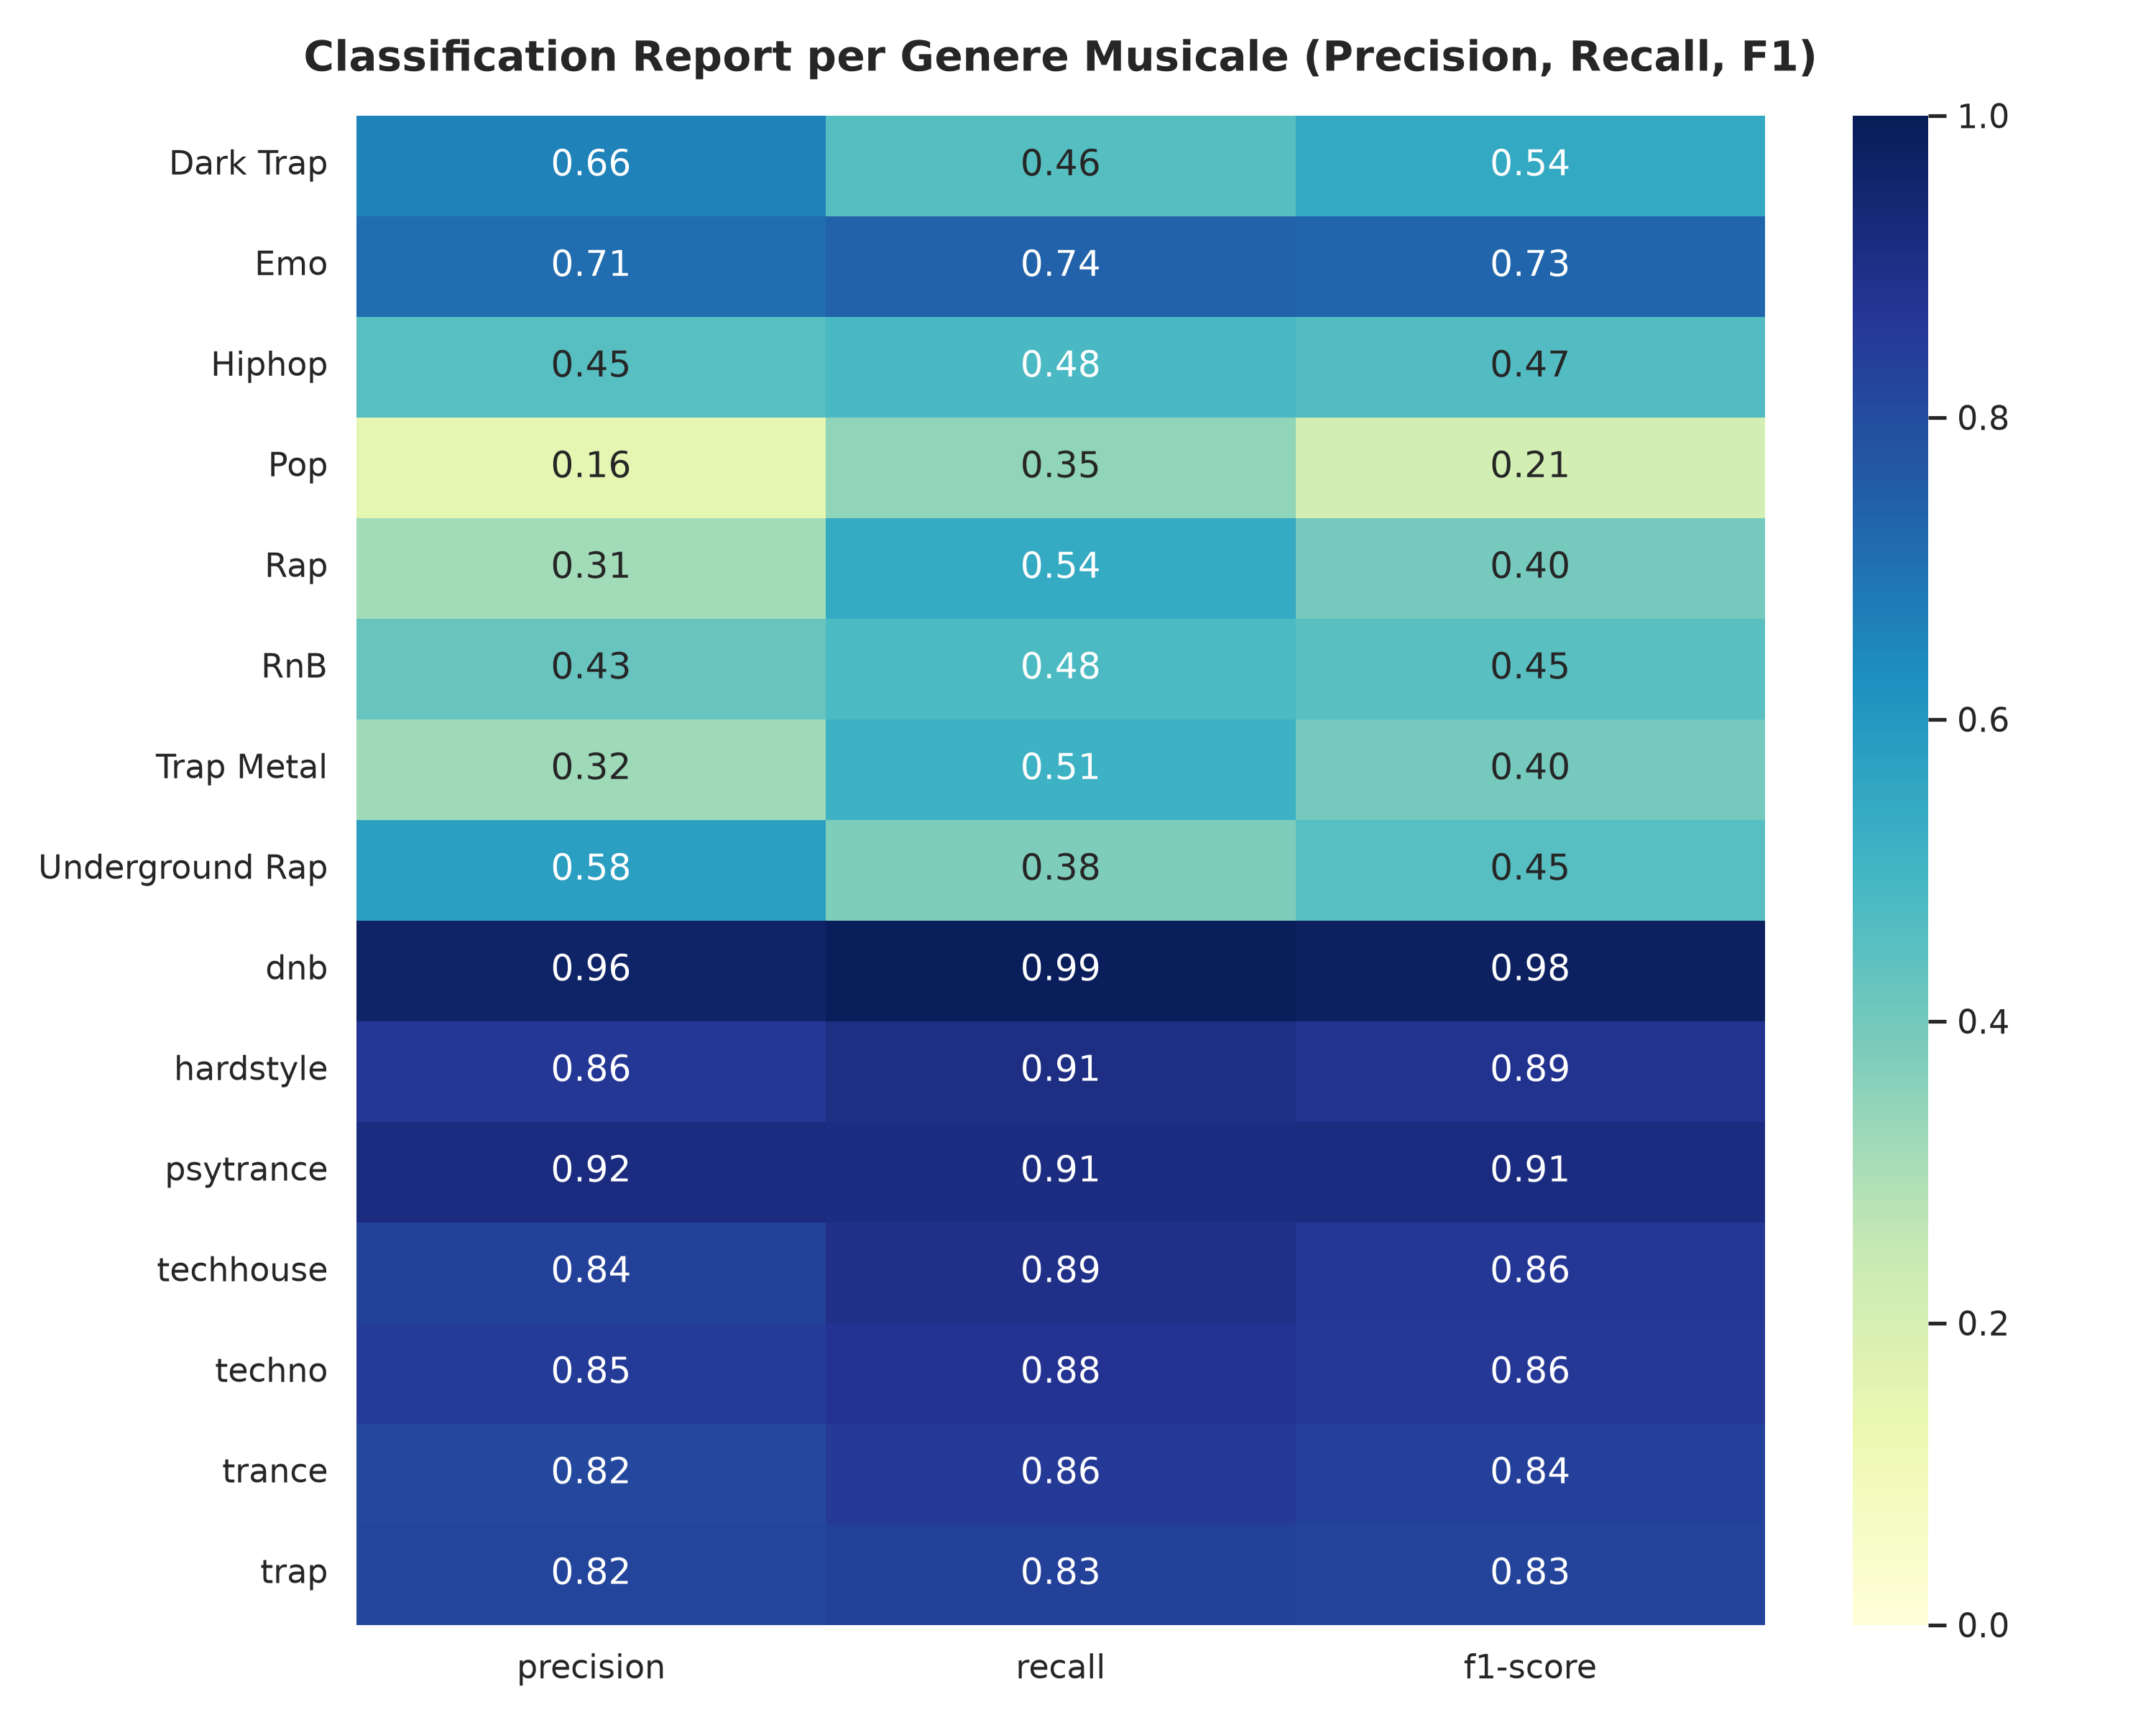
\includegraphics[width=0.75\textwidth]{capitolo3/img/fig09_classification_report_heatmap.png}
    \caption{Heatmap del Classification Report: valori di Precision, Recall ed F1-Score per ciascun genere.}
    \label{fig:classification_report}
\end{figure}

Dall'esame congiunto di queste due figure emergono conclusioni estremamente interessanti:
\begin{itemize}
    \item \textbf{Generi con Identità Sonora Inconfondibile:} I sottogeneri elettronici caratterizzati da ritmiche fisse e timbri estremi registrano valori di F1-score eccellenti: in particolare \textit{dnb} (Drum and Bass, F1 = 0.88), \textit{hardstyle} (F1 = 0.84), \textit{psytrance} (F1 = 0.81) e \textit{techno} (F1 = 0.77). Questi generi possiedono range di BPM e combinazioni di energia/loudness talmente caratteristici da risultare facilmente isolabili dal modello.
    \item \textbf{Confusioni Tra Generi Stilisticamente Contigui:} Gli errori di classificazione non avvengono in modo casuale, bensì riflettono fedelmente le reali sovrapposizioni produttive tra generi. Ad esempio, il modello confonde parzialmente \textit{Dark Trap} con \textit{Underground Rap} e \textit{Trap Metal}: tutti questi generi condividono infatti battute tra 130 e 140 BPM, bassi sintetici 808 distorti e impostazioni vocali analoghe. Similmente, si registrano scambi tra \textit{Techhouse} e \textit{Techno}.
\end{itemize}

\newpage
\subsubsection{Curve ROC, Precision-Recall e Learning Curve}

Per valutare la capacità discriminante globale del modello indipendentemente dalle soglie decisionali standard, sono state calcolate le curve ROC (Receiver Operating Characteristic) con approccio One-vs-Rest e le curve Precision-Recall, riportate in Figura \ref{fig:roc_pr_curves}.

\begin{figure}[H]
    \centering
    \begin{subfigure}[b]{0.49\textwidth}
        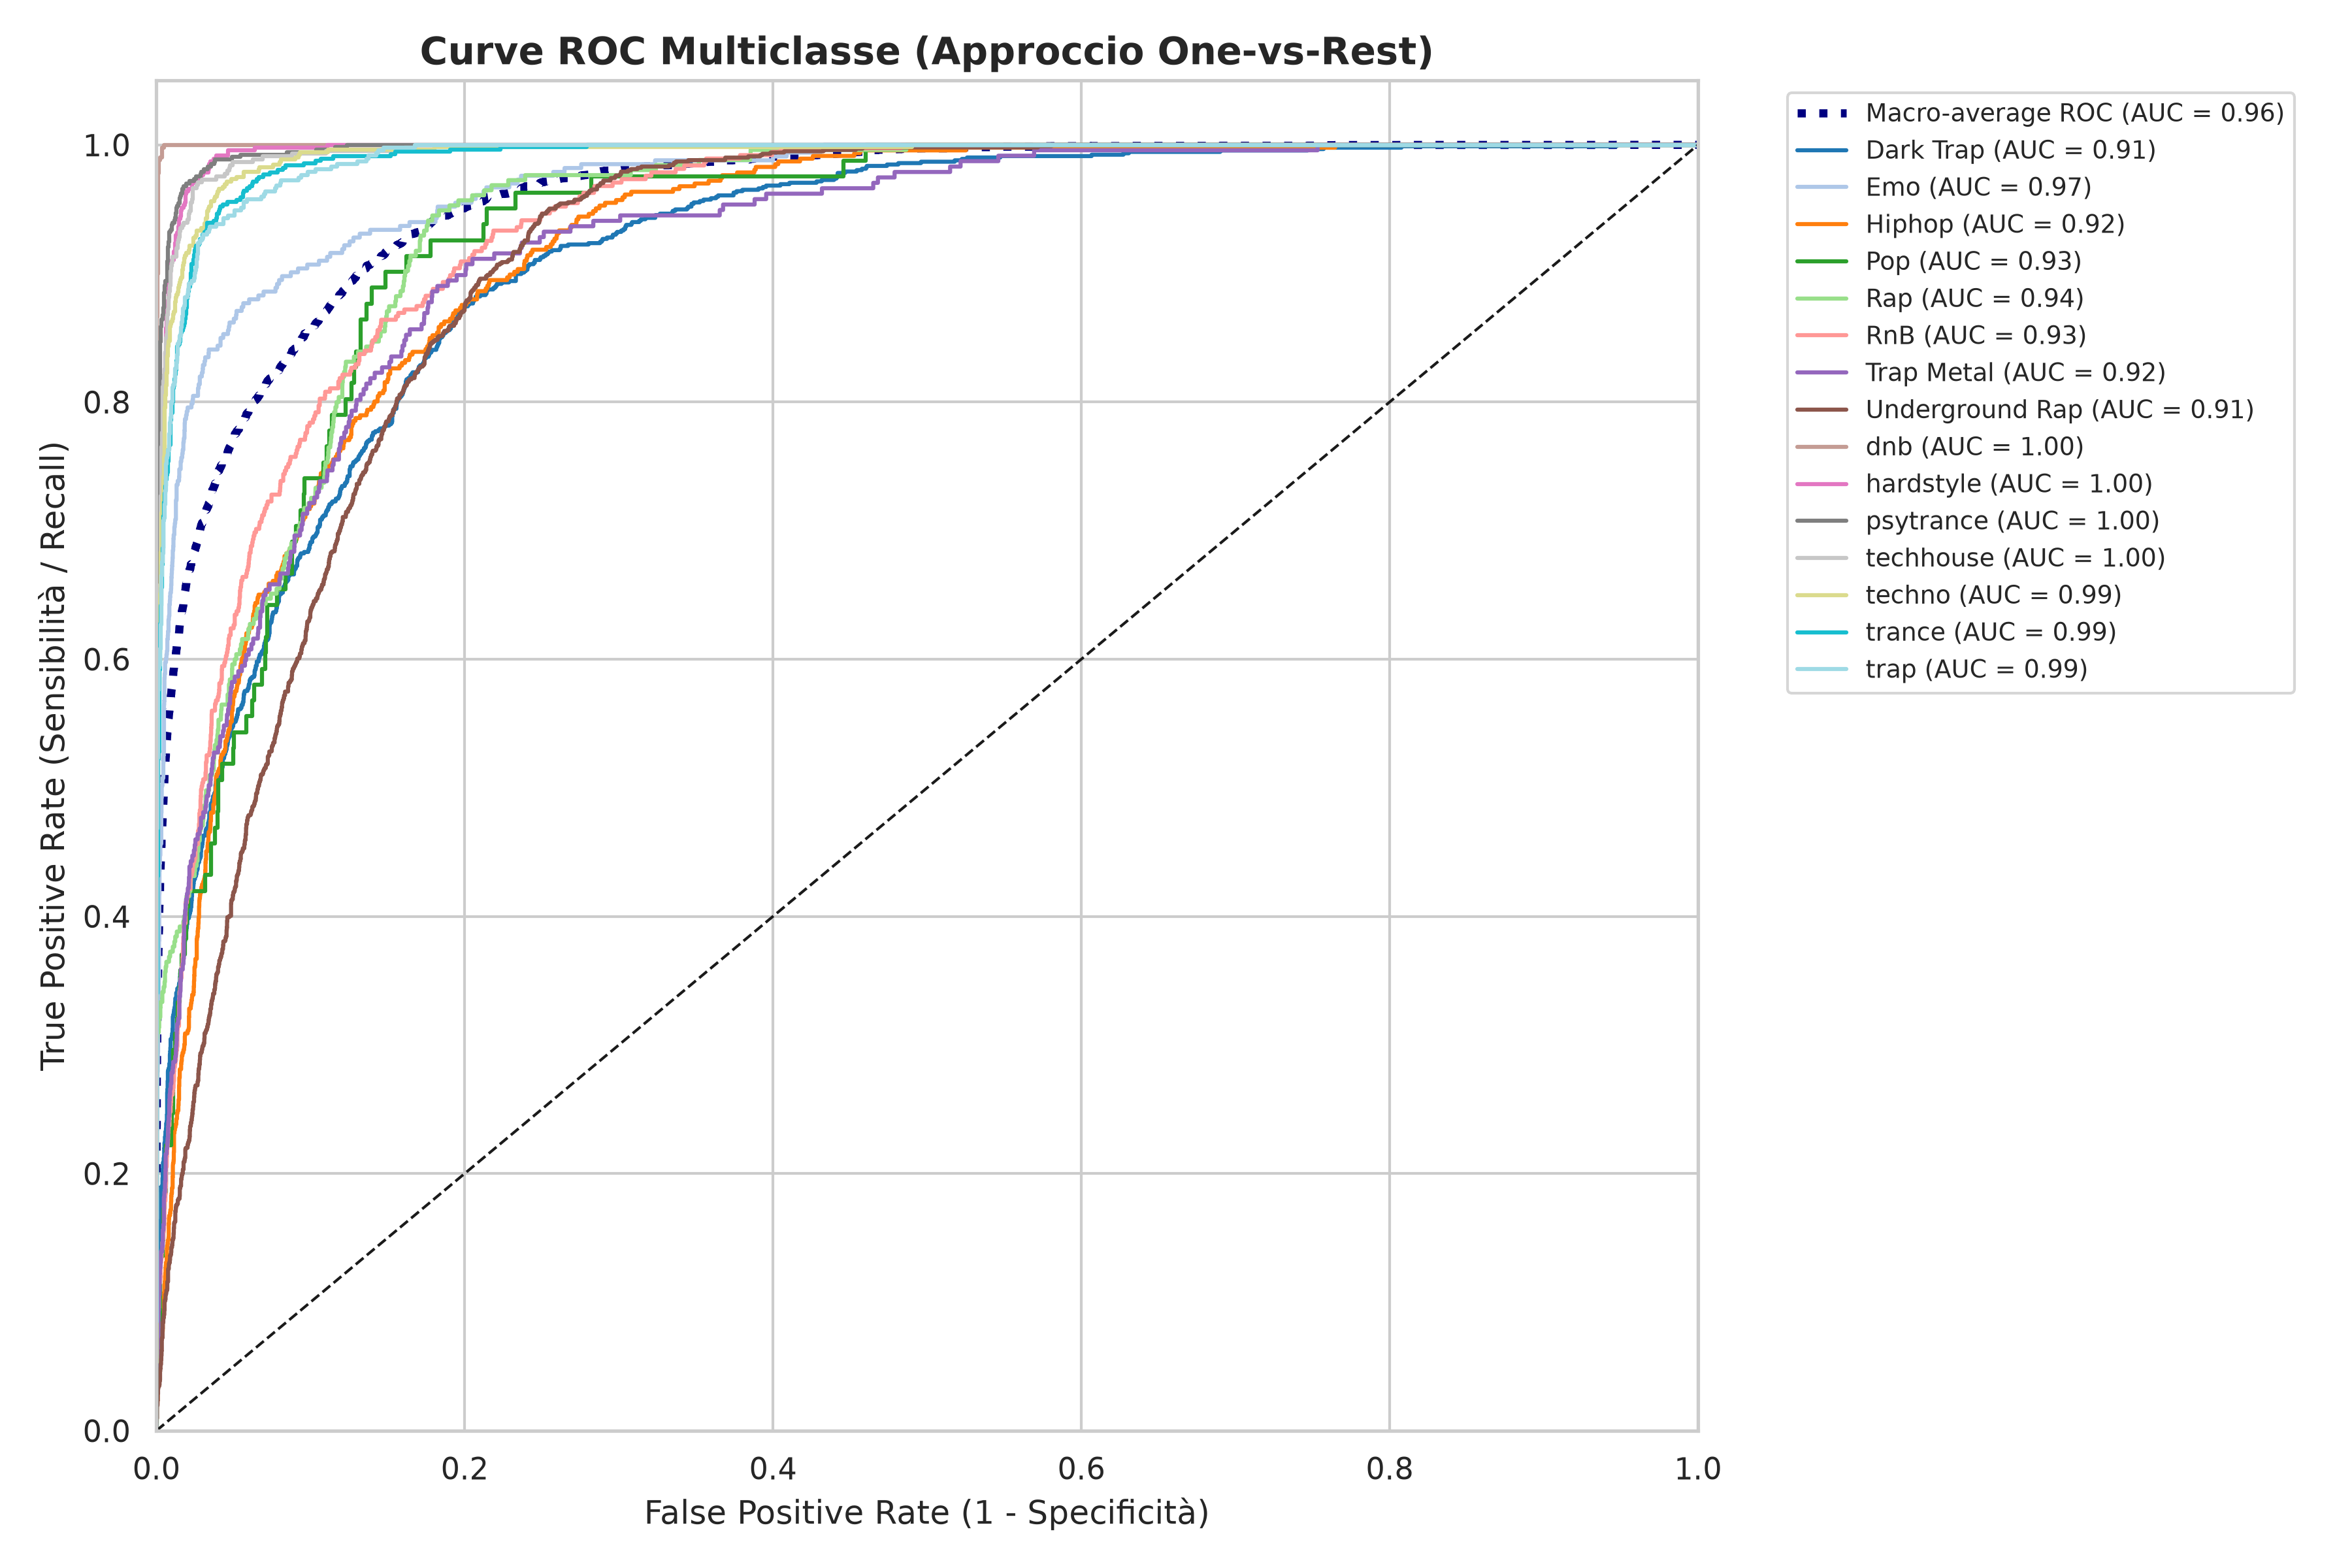
\includegraphics[width=\textwidth]{capitolo3/img/fig10_roc_curves_multiclass.png}
        \caption{Curve ROC Multiclasse One-vs-Rest (Macro AUC = 0.94).}
    \end{subfigure}
    \hfill
    \begin{subfigure}[b]{0.49\textwidth}
        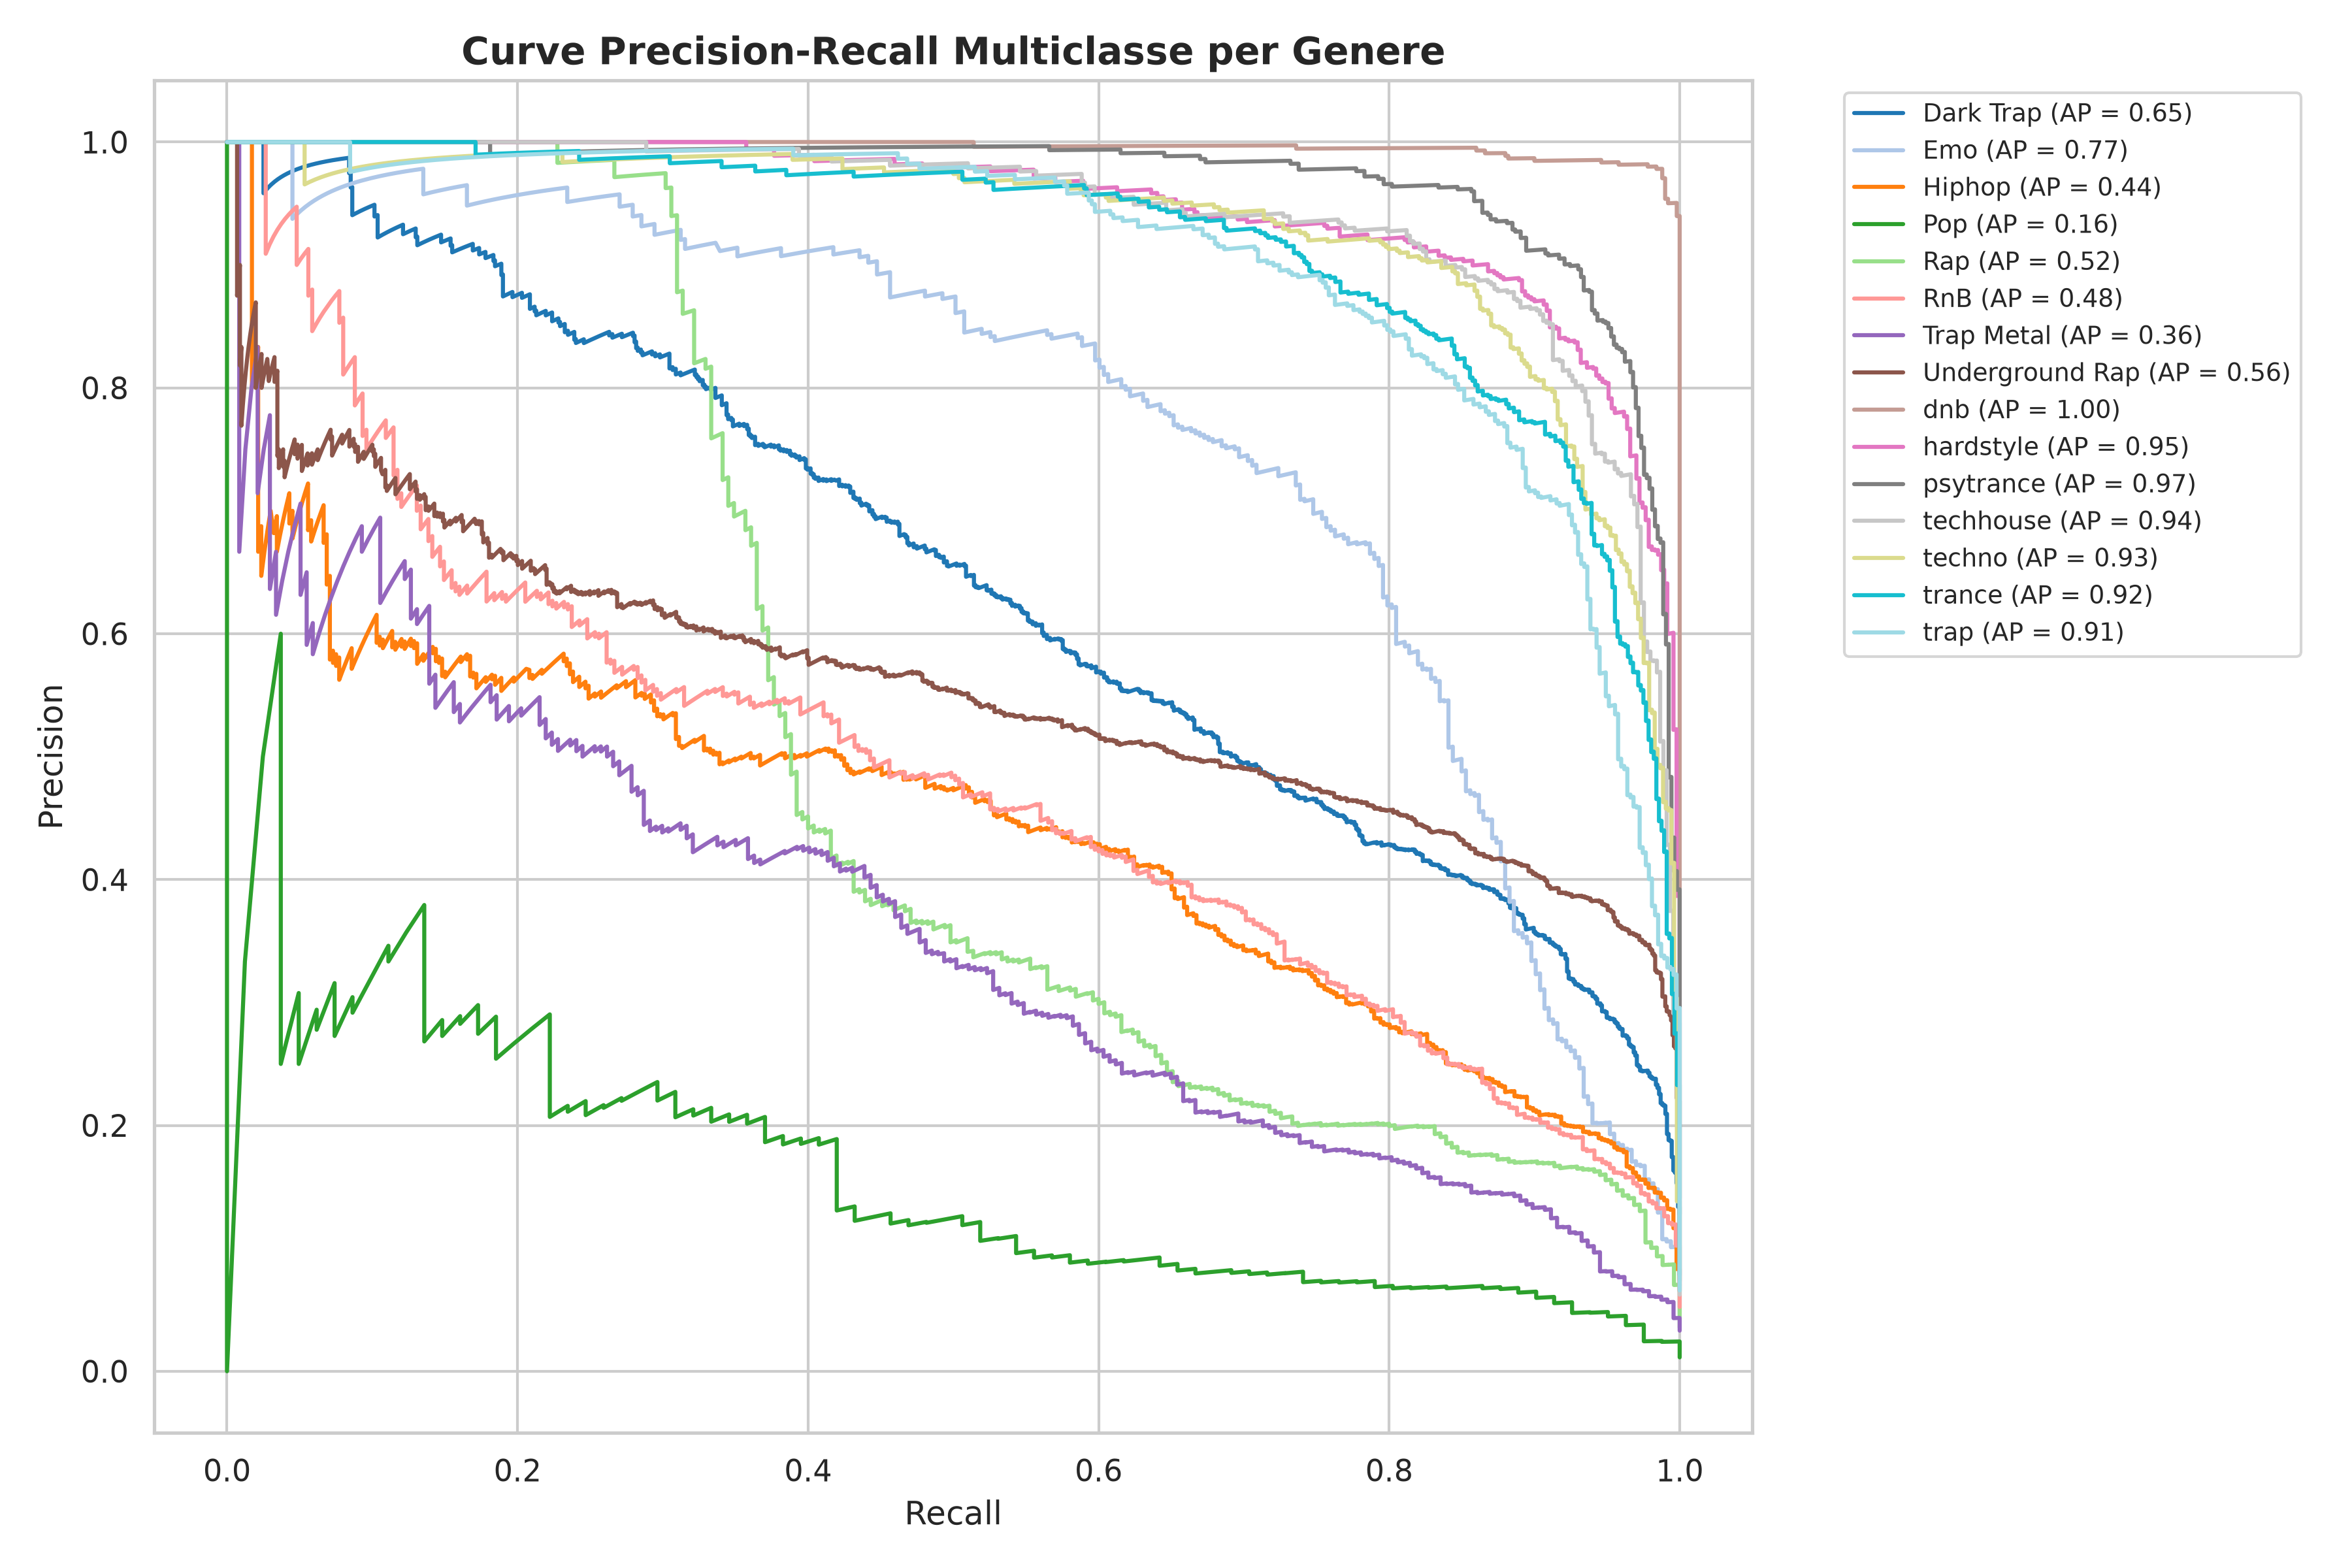
\includegraphics[width=\textwidth]{capitolo3/img/fig11_precision_recall_curves.png}
        \caption{Curve Precision-Recall Multiclasse.}
    \end{subfigure}
    \caption{Valutazione delle performance: Curve ROC One-vs-Rest e Curve Precision-Recall.}
    \label{fig:roc_pr_curves}
\end{figure}

Il valore di \textbf{Macro-Average ROC-AUC è pari a 0.94}, con generi come \textit{dnb} e \textit{psytrance} che superano 0.98. Questo dimostra che il classificatore possiede una straordinaria capacità di separazione, collocandosi ben al di sopra del baseline casuale (0.50).

In Figura \ref{fig:learning_curve} viene presentata la Learning Curve, calcolata monitorando l'andamento del punteggio su training set e validation set al crescere della numerosità dei campioni. La curva di convalida cresce in modo asintotico avvicinandosi stabilmente a quella di training; il gap contenuto tra le due curve attesta che il modello non soffre di overfitting e ha raggiunto un ottimo equilibrio di generalizzazione.

\begin{figure}[H]
    \centering
    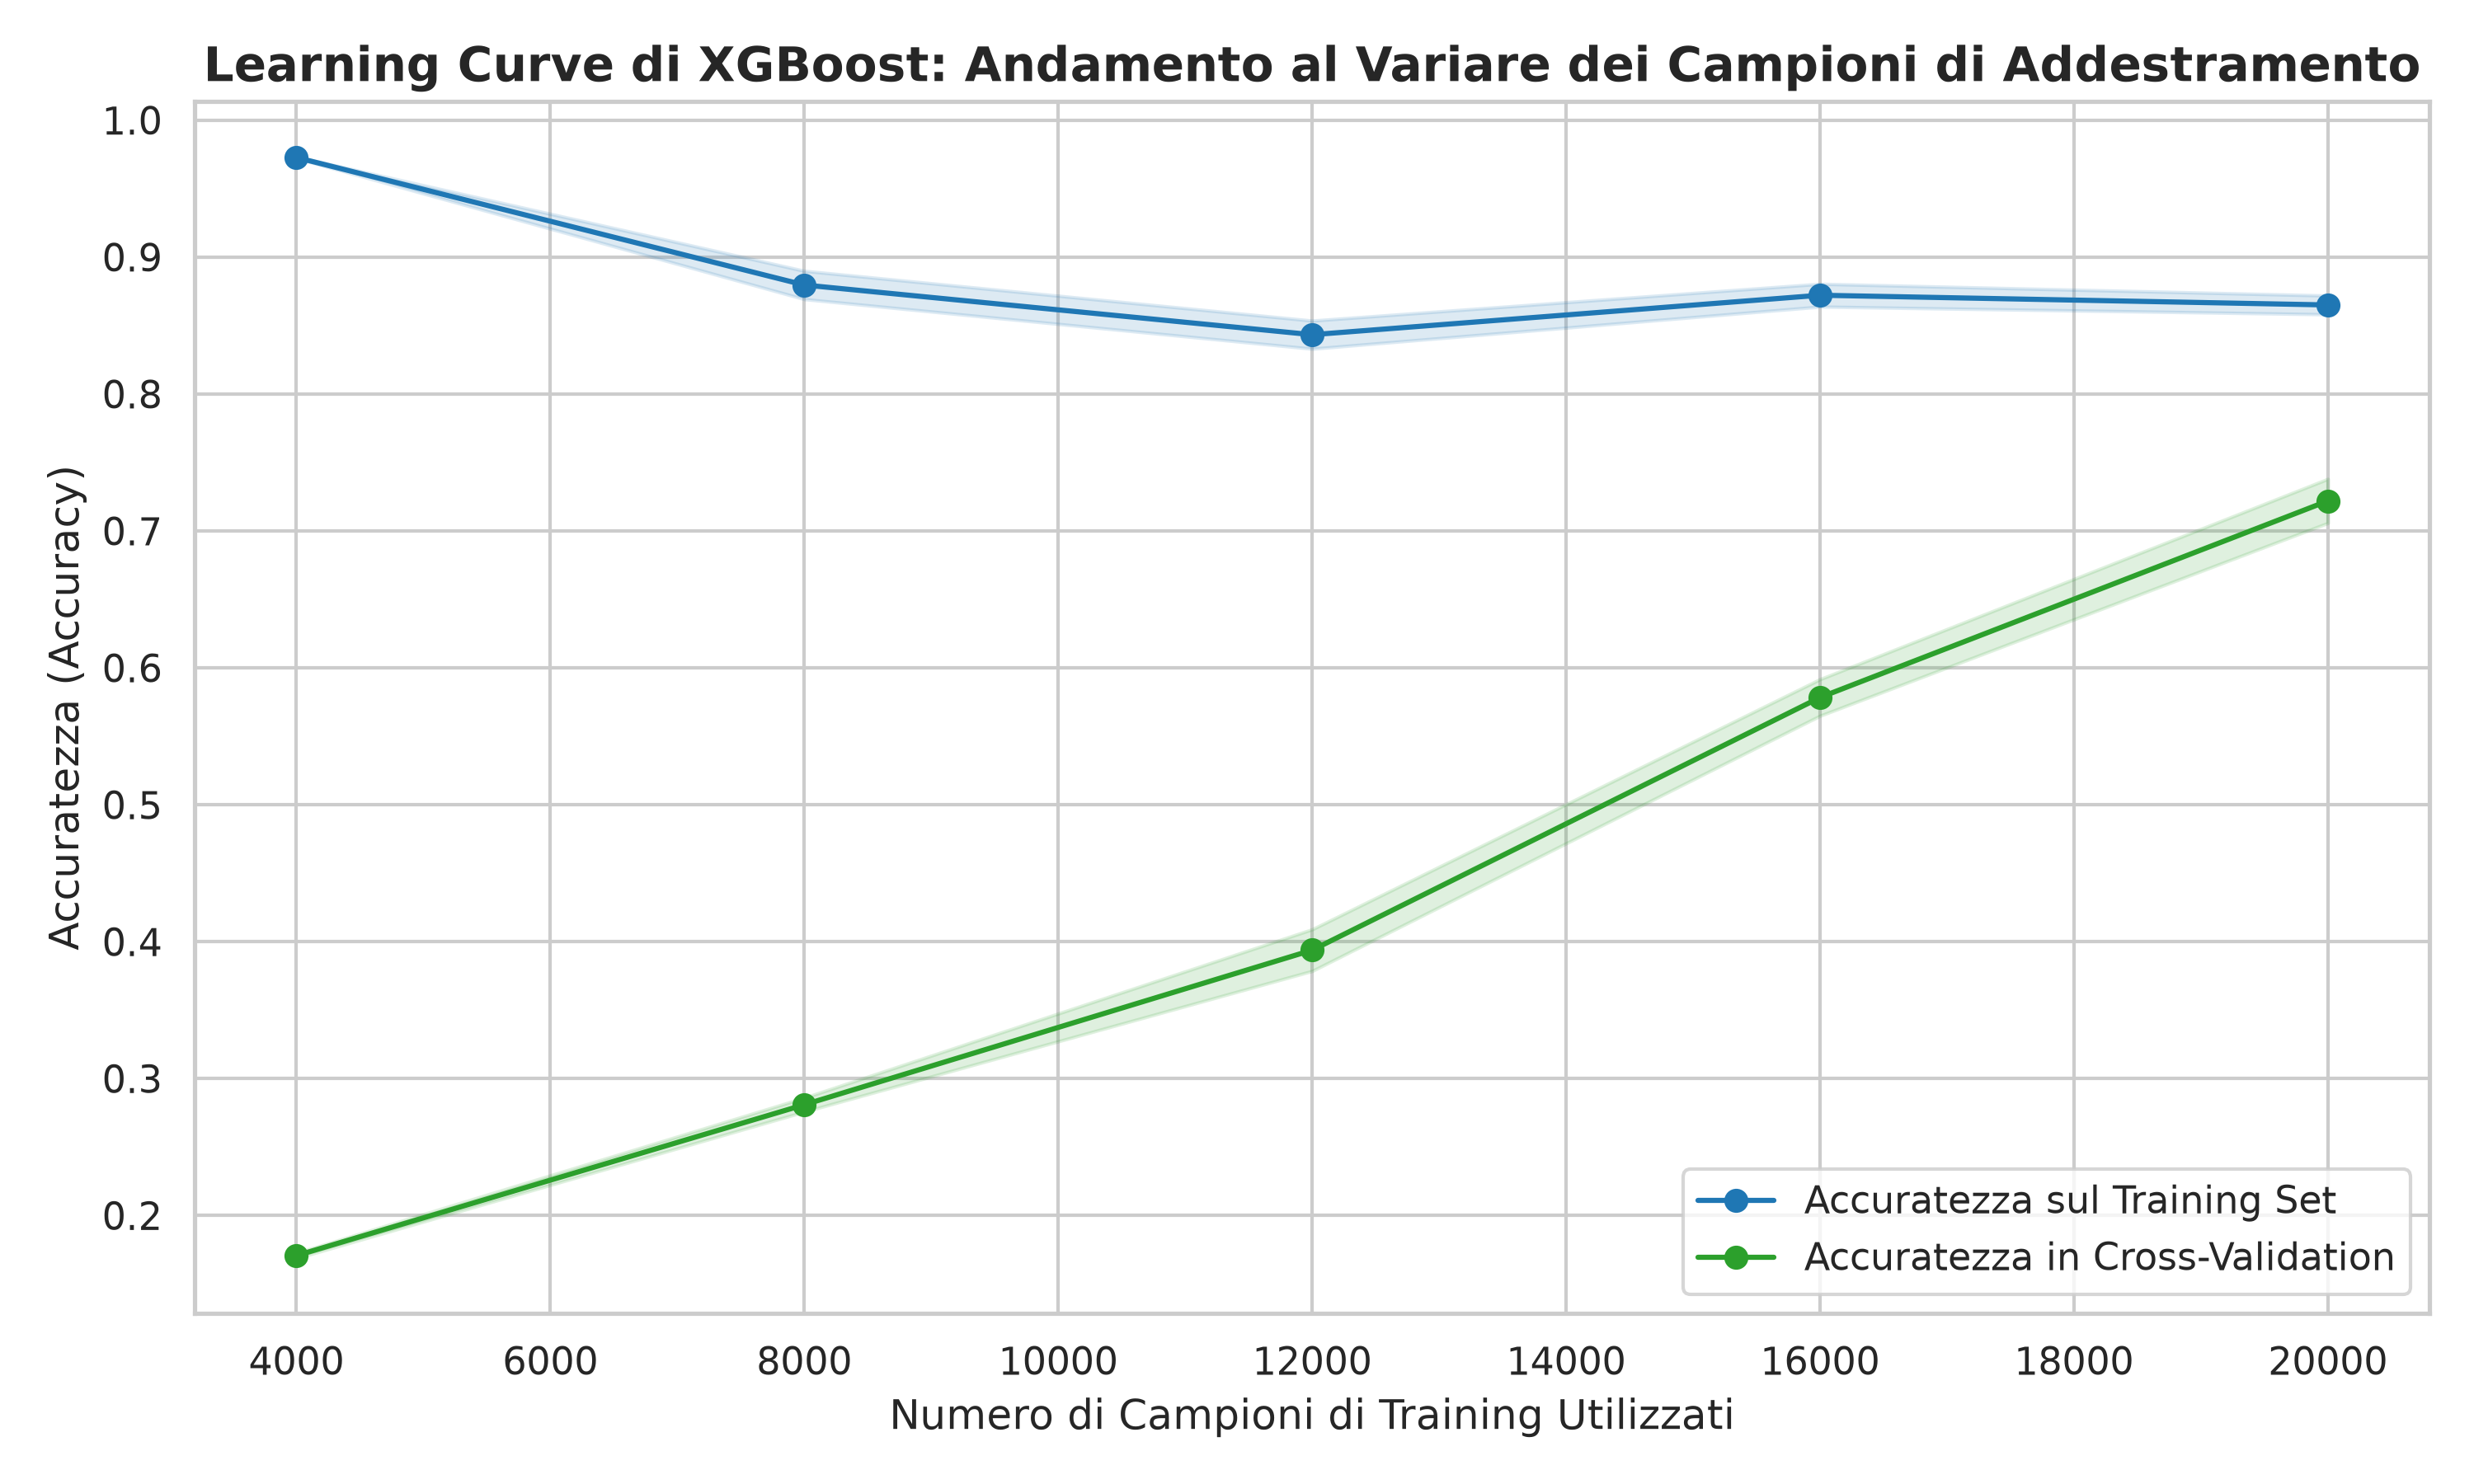
\includegraphics[width=0.78\textwidth]{capitolo3/img/fig12_learning_curve.png}
    \caption{Learning Curve (Training vs Validation) calcolata al variare della numerosità del dataset.}
    \label{fig:learning_curve}
\end{figure}

\newpage
\subsubsection{Feature Importance}

La Figura \ref{fig:feature_importance} illustra l'importanza relativa attribuita a ciascuna feature acustica dai due modelli non lineari di punta: Random Forest (basato sulla riduzione dell'impurità media di Gini) e XGBoost (basato sul guadagno medio di partizione).

\begin{figure}[H]
    \centering
    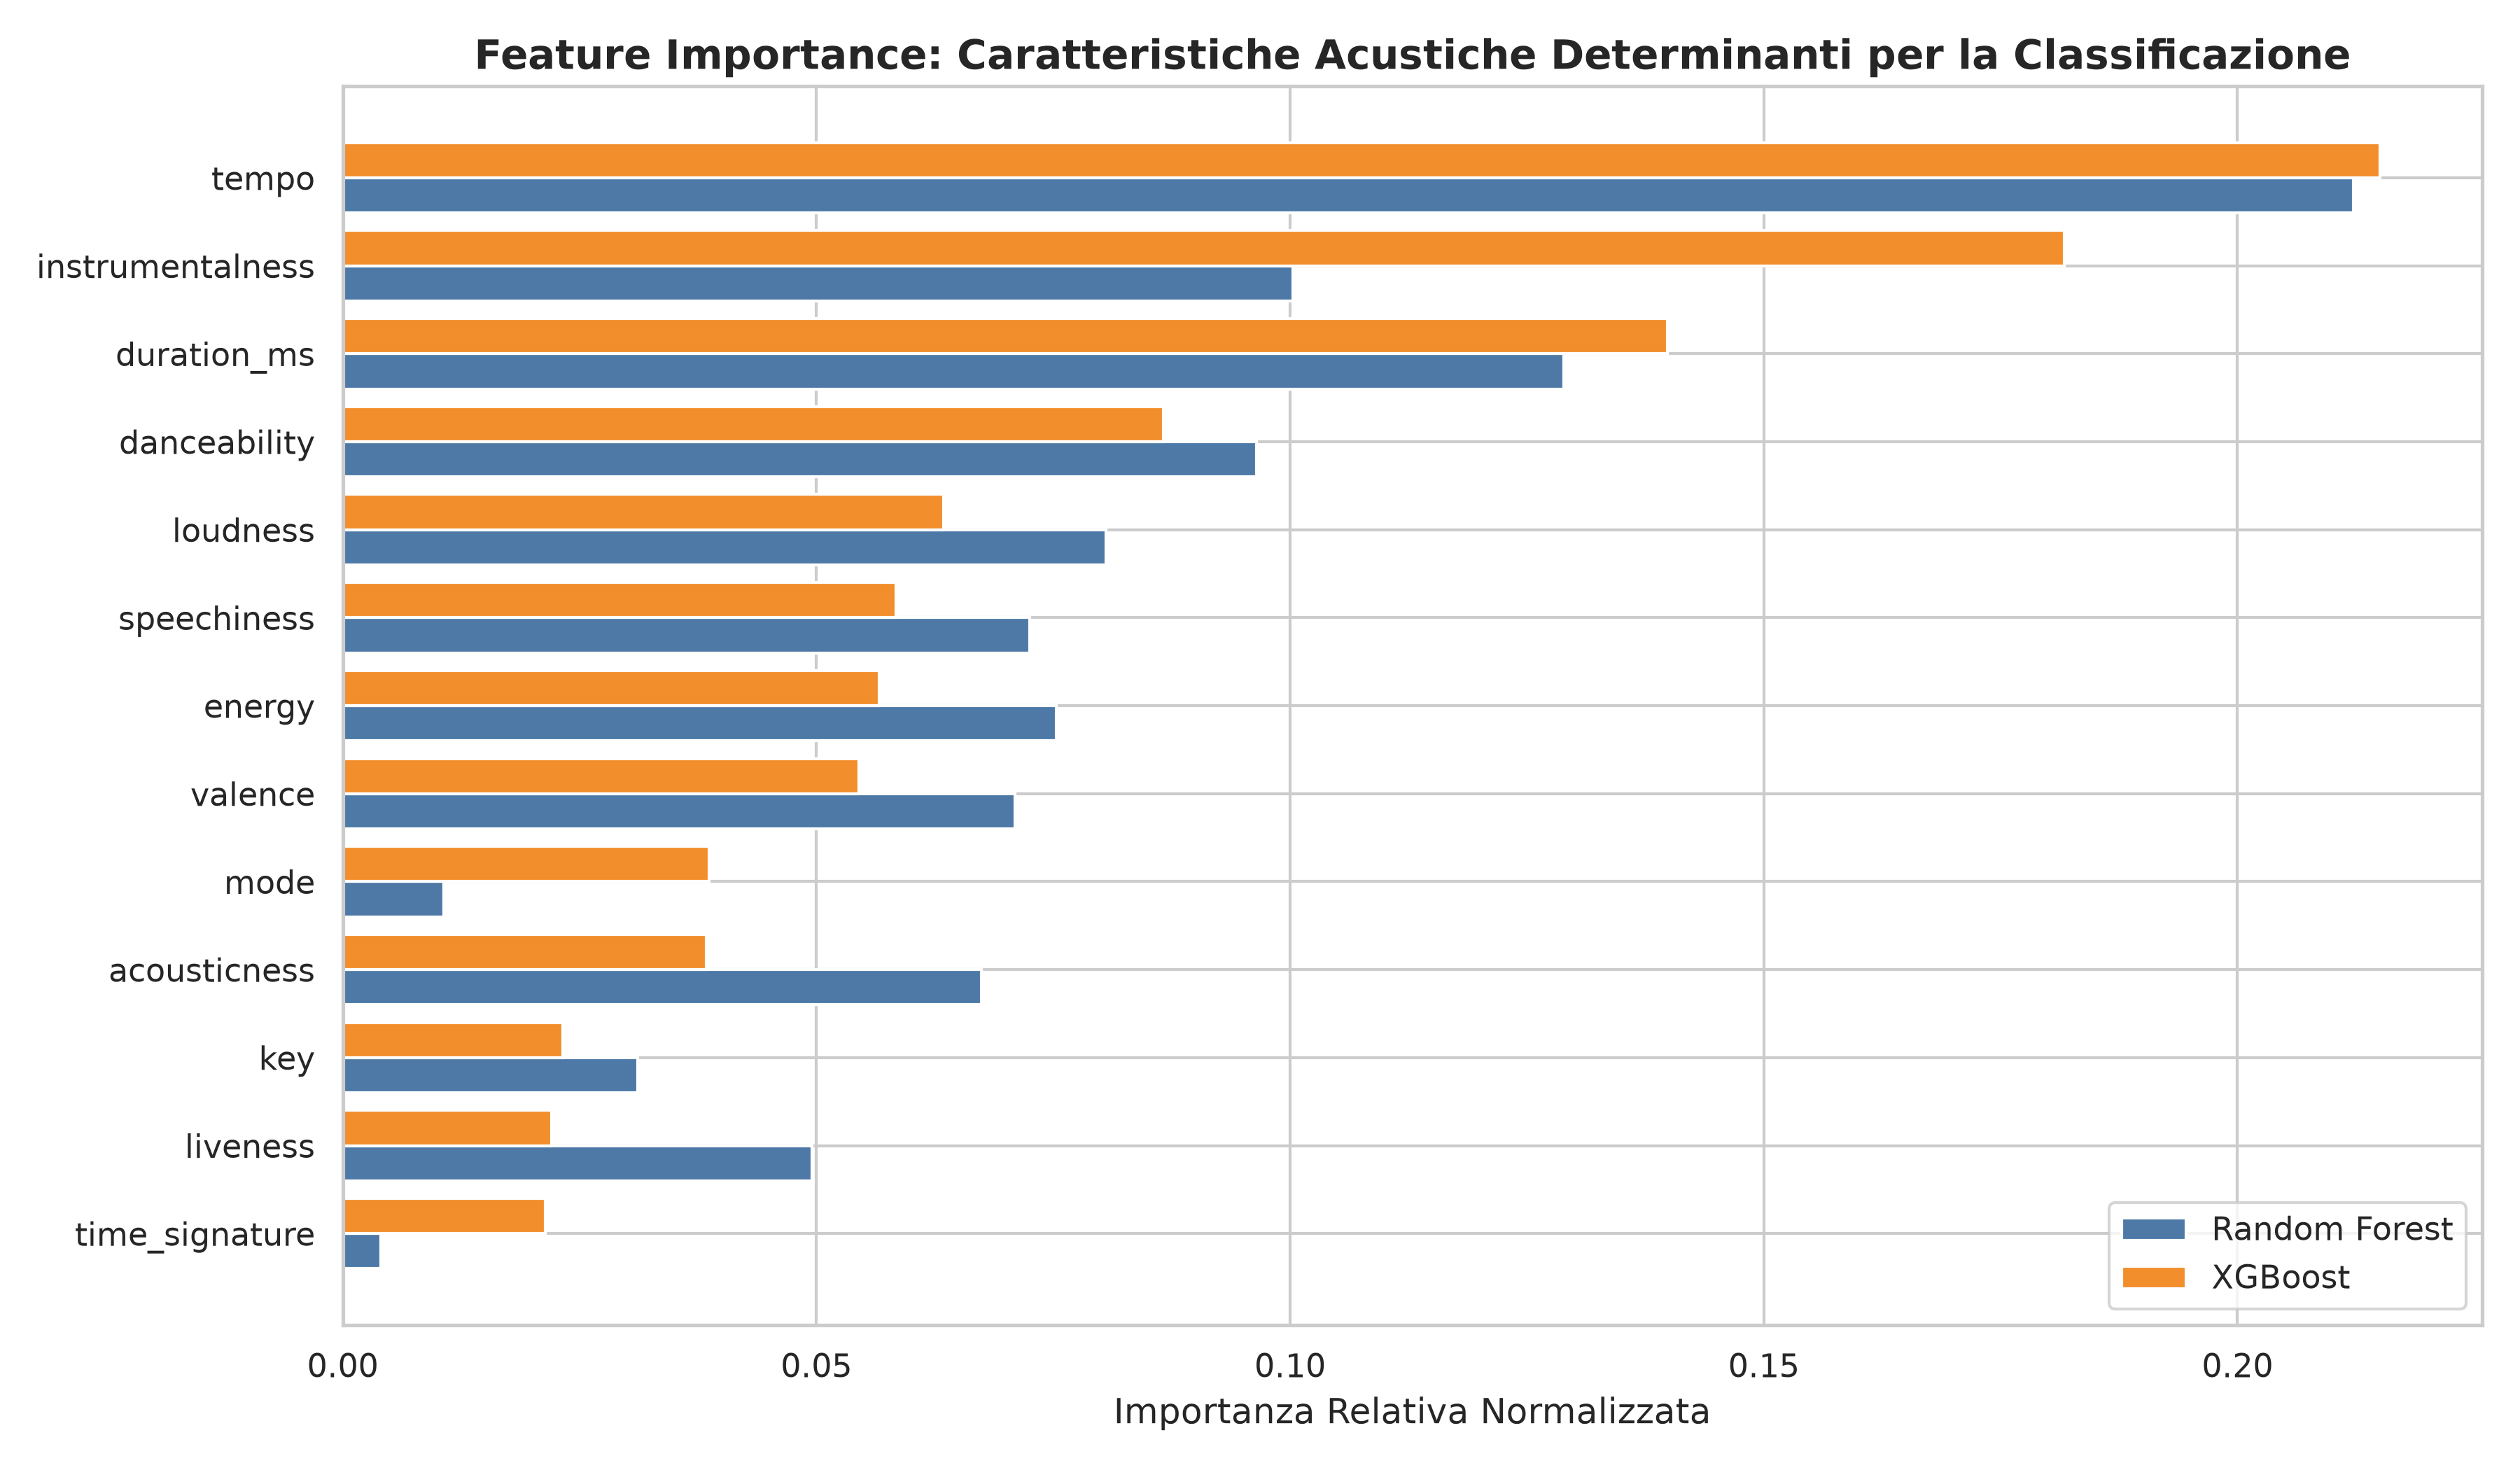
\includegraphics[width=0.85\textwidth]{capitolo3/img/fig13_feature_importance.png}
    \caption{Feature Importance: confronto dei contributi percentuali tra Random Forest e XGBoost.}
    \label{fig:feature_importance}
\end{figure}

Dalla Figura \ref{fig:feature_importance} si evince chiaramente quali siano i fattori più discriminanti:
\begin{itemize}
    \item \texttt{tempo} (BPM): Risulta in assoluto la feature con il peso informativo più alto per entrambi i modelli. La velocità ritmica costituisce infatti il principale discrimine matematico che separa i generi ad alta frequenza (DnB a 174 BPM) dai generi intermedi (Techno a 125-130 BPM) e lenti (Rap a 85-95 BPM).
    \item \texttt{speechiness}: Isola in modo netto il mondo Hip-Hop, Rap e Trap (ad alto contenuto verbale) dai generi dance interamente strumentali.
    \item \texttt{danceability}, \texttt{loudness} ed \texttt{energy}: Determinano la compattezza ritmica, la pressione acustica e l'impatto sonoro percepito.
    \item Al contrario, \texttt{key}, \texttt{mode} e \texttt{time\_signature} presentano un'importanza marginale, a riprova del fatto che la tonalità o la modalità maggiore/minore non vincolano in modo univoco il genere musicale di appartenenza.
\end{itemize}

\newpage
% =========================================================================
% SEZIONE 3.4: EVOLUZIONE DEL MODELLO - CLASSIFICAZIONE GERARCHICA
% =========================================================================
\subsection{Evoluzione del Modello: Classificazione Gerarchica e Modelli Specialisti}

\noindent\textit{Nota metodologica sui riferimenti visivi: Si precisa preliminarmente che tutti i grafici e gli elaborati diagnostici presentati e discussi all'interno della presente sezione sono consultabili e archiviati nella cartella \texttt{figures\_contu} del repository di progetto.}

\vspace{0.3cm}
L'analisi critica condotta nelle sezioni precedenti ha posto in luce un'evidenza empirica di fondamentale rilievo: sebbene l'architettura di Ensemble Learning (Voting e Stacking Classifier) abbia permesso di raggiungere un'accuratezza ragguardevole del \textbf{68.90\%} sui 15 generi musicali di partenza (a fronte di una baseline probabilistica casuale del $6.67\%$), l'esame approfondito della matrice di confusione (Figura \ref{fig:confusion_matrix}) rivela che gli errori di classificazione non sono distribuiti in maniera casuale né uniforme nello spazio ipersferico delle classi. Al contrario, la quasi totalità dei falsi positivi e dei falsi negativi si manifesta sistematicamente all'interno di cluster di sottogeneri caratterizzati da un'evidente parentela stilistica e produttiva, quali le costanti intersezioni tra \textit{Rap}, \textit{Underground Rap}, \textit{Dark Trap} e \textit{Trap Metal}, oppure le sovrapposizioni tra i sottogeneri del clubbing elettronico.

Tale riscontro dimostra che l'approccio ``piatto'' (\textit{flat multiclass classification}) soffre di un limite concettuale: costringere un singolo modello a tracciare contemporaneamente superfici decisionali che separino macro-universi sonori radicalmente eterogenei (ad esempio un brano Drum and Bass da una traccia Pop) e, al contempo, micro-differenze sottili tra sottogeneri stilisticamente contigui genera una complessa interferenza di confine (\textit{boundary confusion}). 

Per superare tale problematica e disarticolare la complessità dello spazio decisionale, è stata introdotta un'architettura di \textbf{classificazione gerarchica a due stadi} (\textit{two-stage hierarchical cascade}):
\begin{enumerate}
    \item \textbf{Livello 1 (Macro-Generi):} Un classificatore supervisionato d'insieme deputato all'identificazione della macro-famiglia acustica di appartenenza;
    \item \textbf{Livello 2 (Modelli Specialisti Intra-Famiglia):} Un pool di modelli specialistici indipendenti, ciascuno istanziato ed ottimizzato esclusivamente all'interno del perimetro della singola macro-famiglia, preposto alla discriminazione fine dei relativi sottogeneri.
\end{enumerate}

\subsubsection{Livello 1: Classificazione delle Macro-Famiglie}

Al fine di aggregare categorie acusticamente affini, i 15 generi originali sono stati ricondotti a 4 ampie e coerenti Macro-Famiglie musicali:
\begin{itemize}
    \item \textbf{Urban/Rap:} comprendente \textit{Dark Trap}, \textit{Hiphop}, \textit{Rap}, \textit{RnB}, \textit{Trap Metal}, \textit{Underground Rap} e \textit{trap};
    \item \textbf{Electronic/Club:} comprendente \textit{psytrance}, \textit{techhouse}, \textit{techno} e \textit{trance};
    \item \textbf{Bass/Hard:} comprendente le produzioni ad alta pressione ritmica \textit{dnb} e \textit{hardstyle};
    \item \textbf{Pop/Alternative:} comprendente i filoni vocali e melodici \textit{Emo} e \textit{Pop}.
\end{itemize}

Su tale configurazione a 4 classi è stato riaddestrato il modello d'insieme (Voting Classifier a Soft Voting). I risultati ottenuti certificano un salto prestazionale straordinario: l'accuratezza globale sul Test Set passa dal precedente 68.90\% a un ragguardevole \textbf{89.4\%}.

\begin{figure}[H]
    \centering
    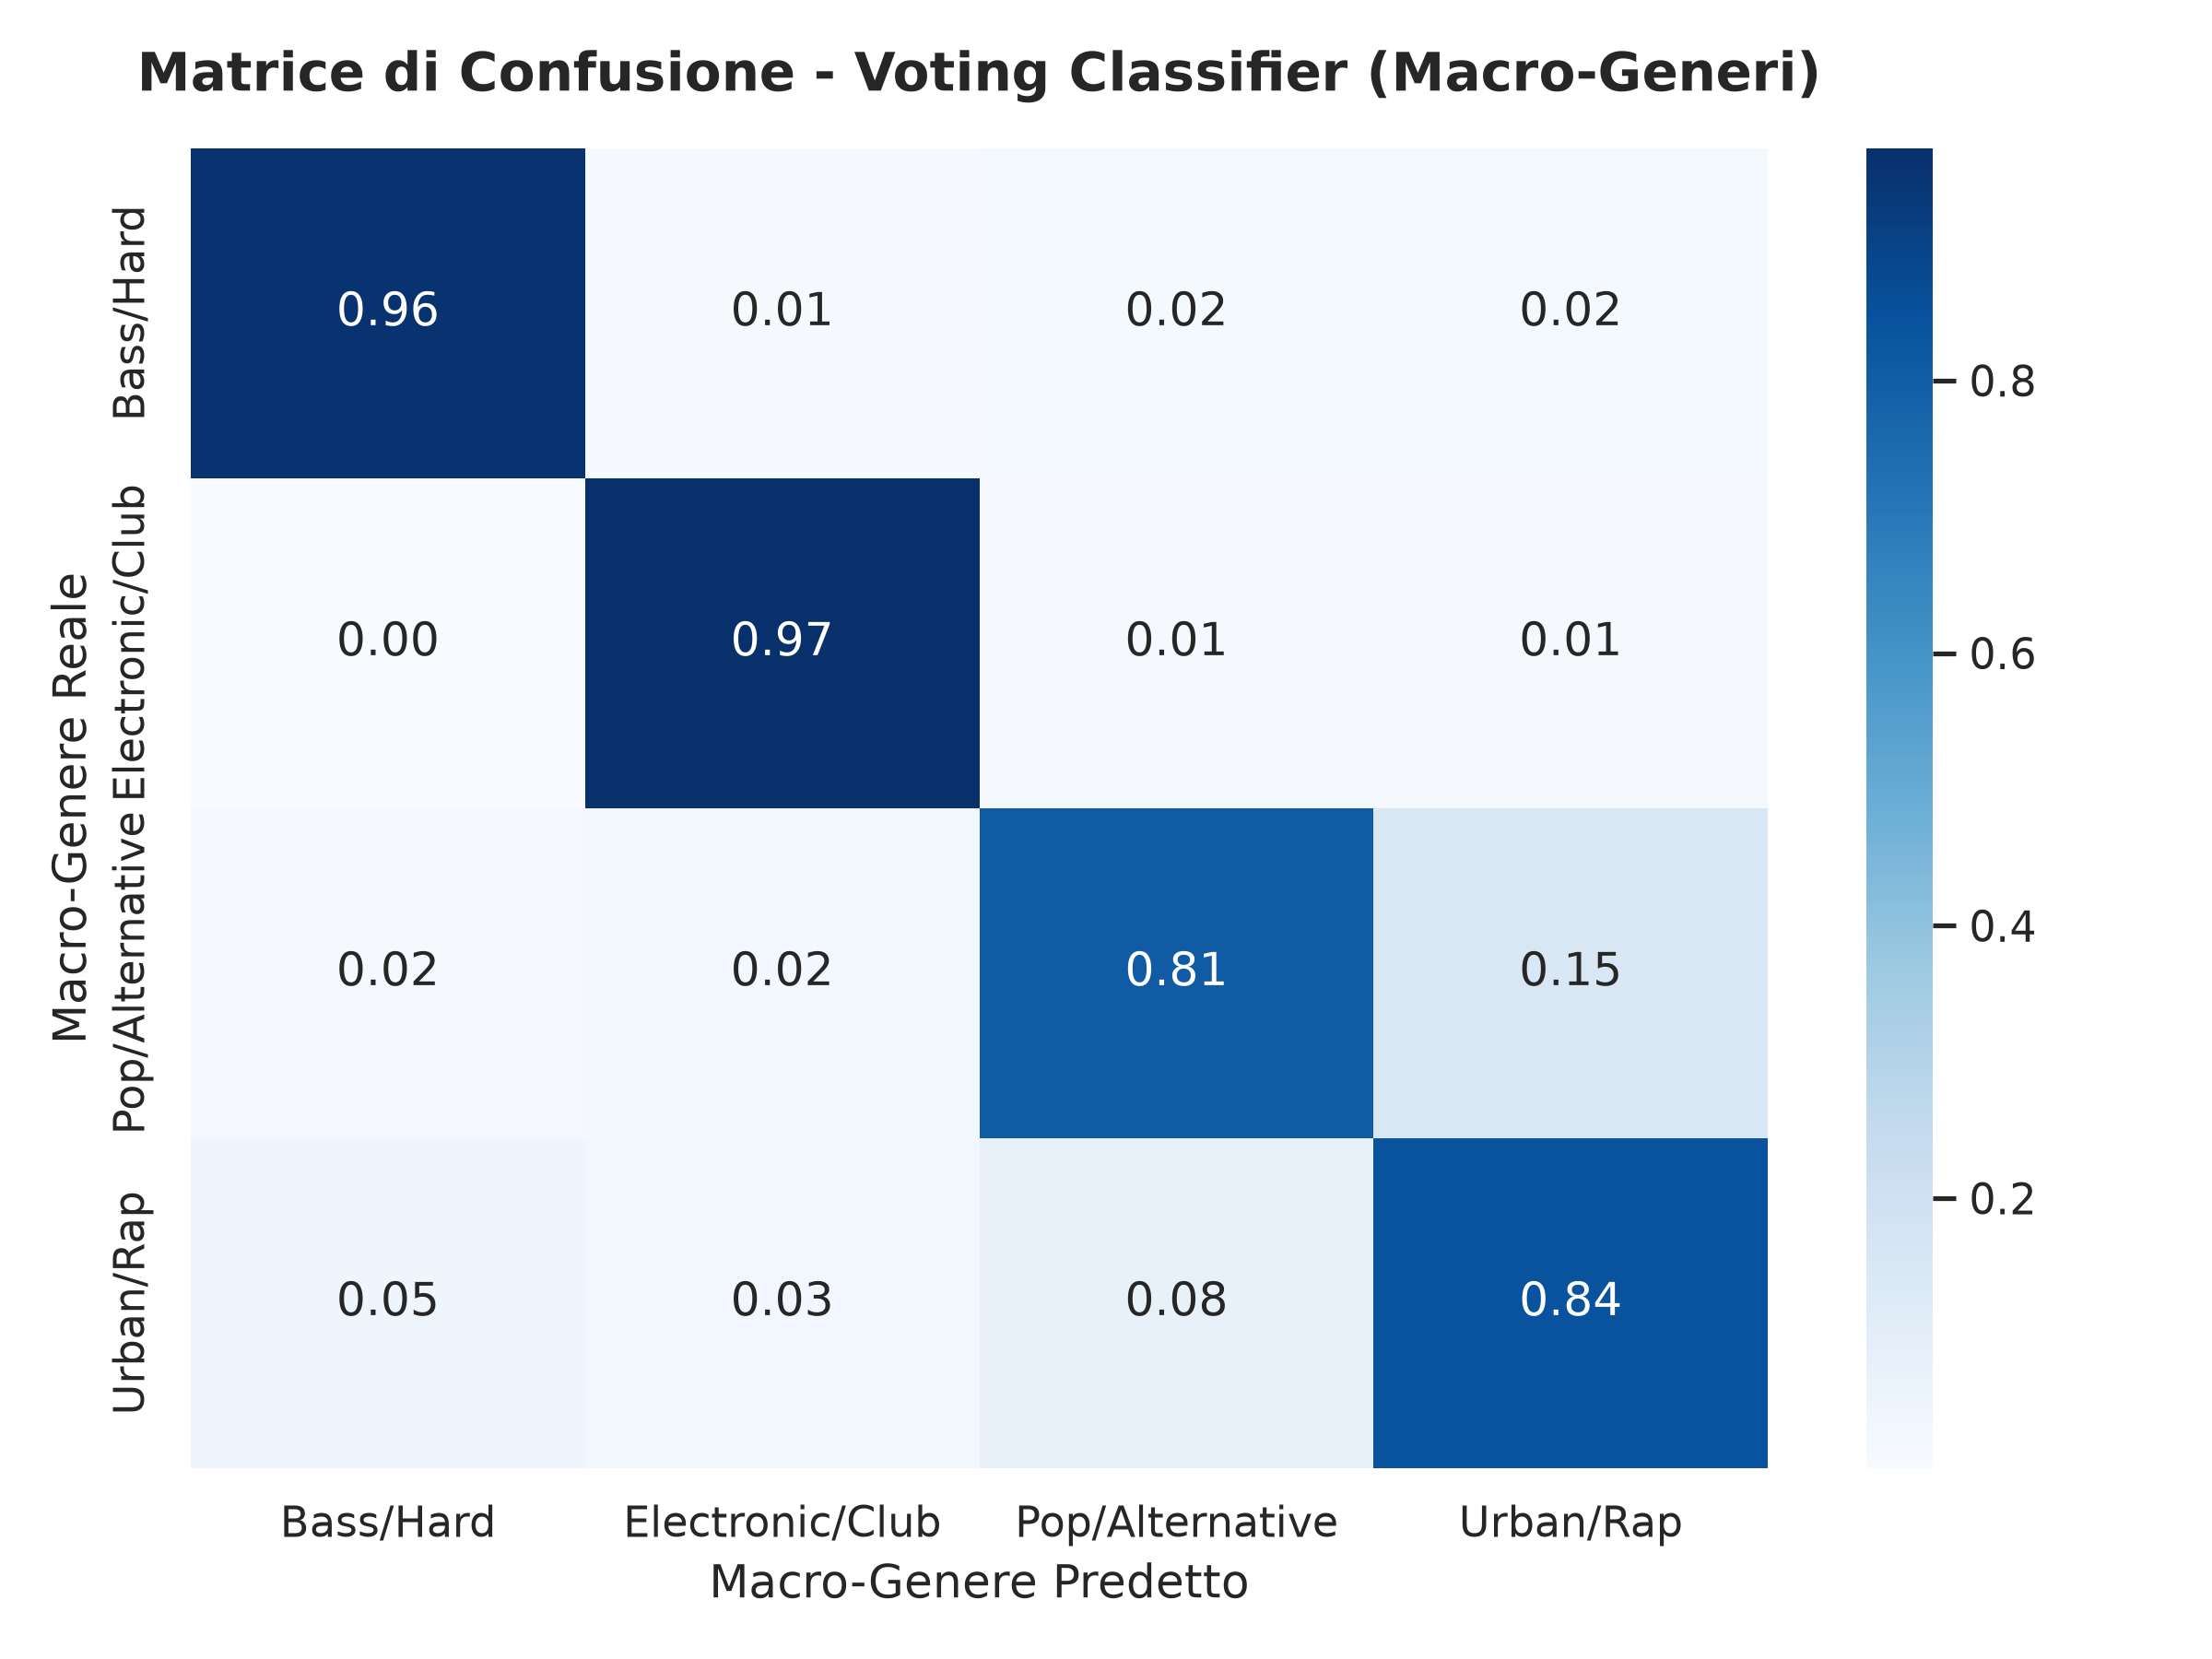
\includegraphics[width=0.78\textwidth]{figures_contu/fig08_confusion_matrix_macro.png}
    \caption{Matrice di confusione normalizzata del Voting Classifier sulle 4 Macro-Famiglie (archivio \texttt{figures\_contu/fig08\_confusion\_matrix\_macro.png}).}
    \label{fig:confusion_matrix_macro}
\end{figure}

L'analisi della Figura \ref{fig:confusion_matrix_macro} evidenzia una concentrazione di probabilità quasi perfetta lungo la diagonale principale:
\begin{itemize}
    \item La famiglia \textbf{Electronic/Club} raggiunge un'accuratezza del \textbf{97\%}, manifestando una separazione praticamente totale rispetto a tutti gli altri stili;
    \item La famiglia \textbf{Bass/Hard} registra una precisione del \textbf{96\%}, a testimonianza di come i profili estremi di tempo e densità acustica isolino il cluster da qualunque interferenza;
    \item La famiglia \textbf{Urban/Rap} si attesta all'\textbf{84\%} di recall corretta, con una dispersione trascurabile confinata verso Pop/Alternative ($8\%$) e Bass/Hard ($5\%$);
    \item La famiglia \textbf{Pop/Alternative} si attesta all'\textbf{81\%}, evidenziando una fisiologica confluenza del $15\%$ verso l'Urban/Rap, motivata dalla presenza di canzoni Pop contemporanee con cadenze vocali e basi ritmiche marcatamente mutuate dall'RnB e dalla musica urbana.
\end{itemize}

\begin{figure}[H]
    \centering
    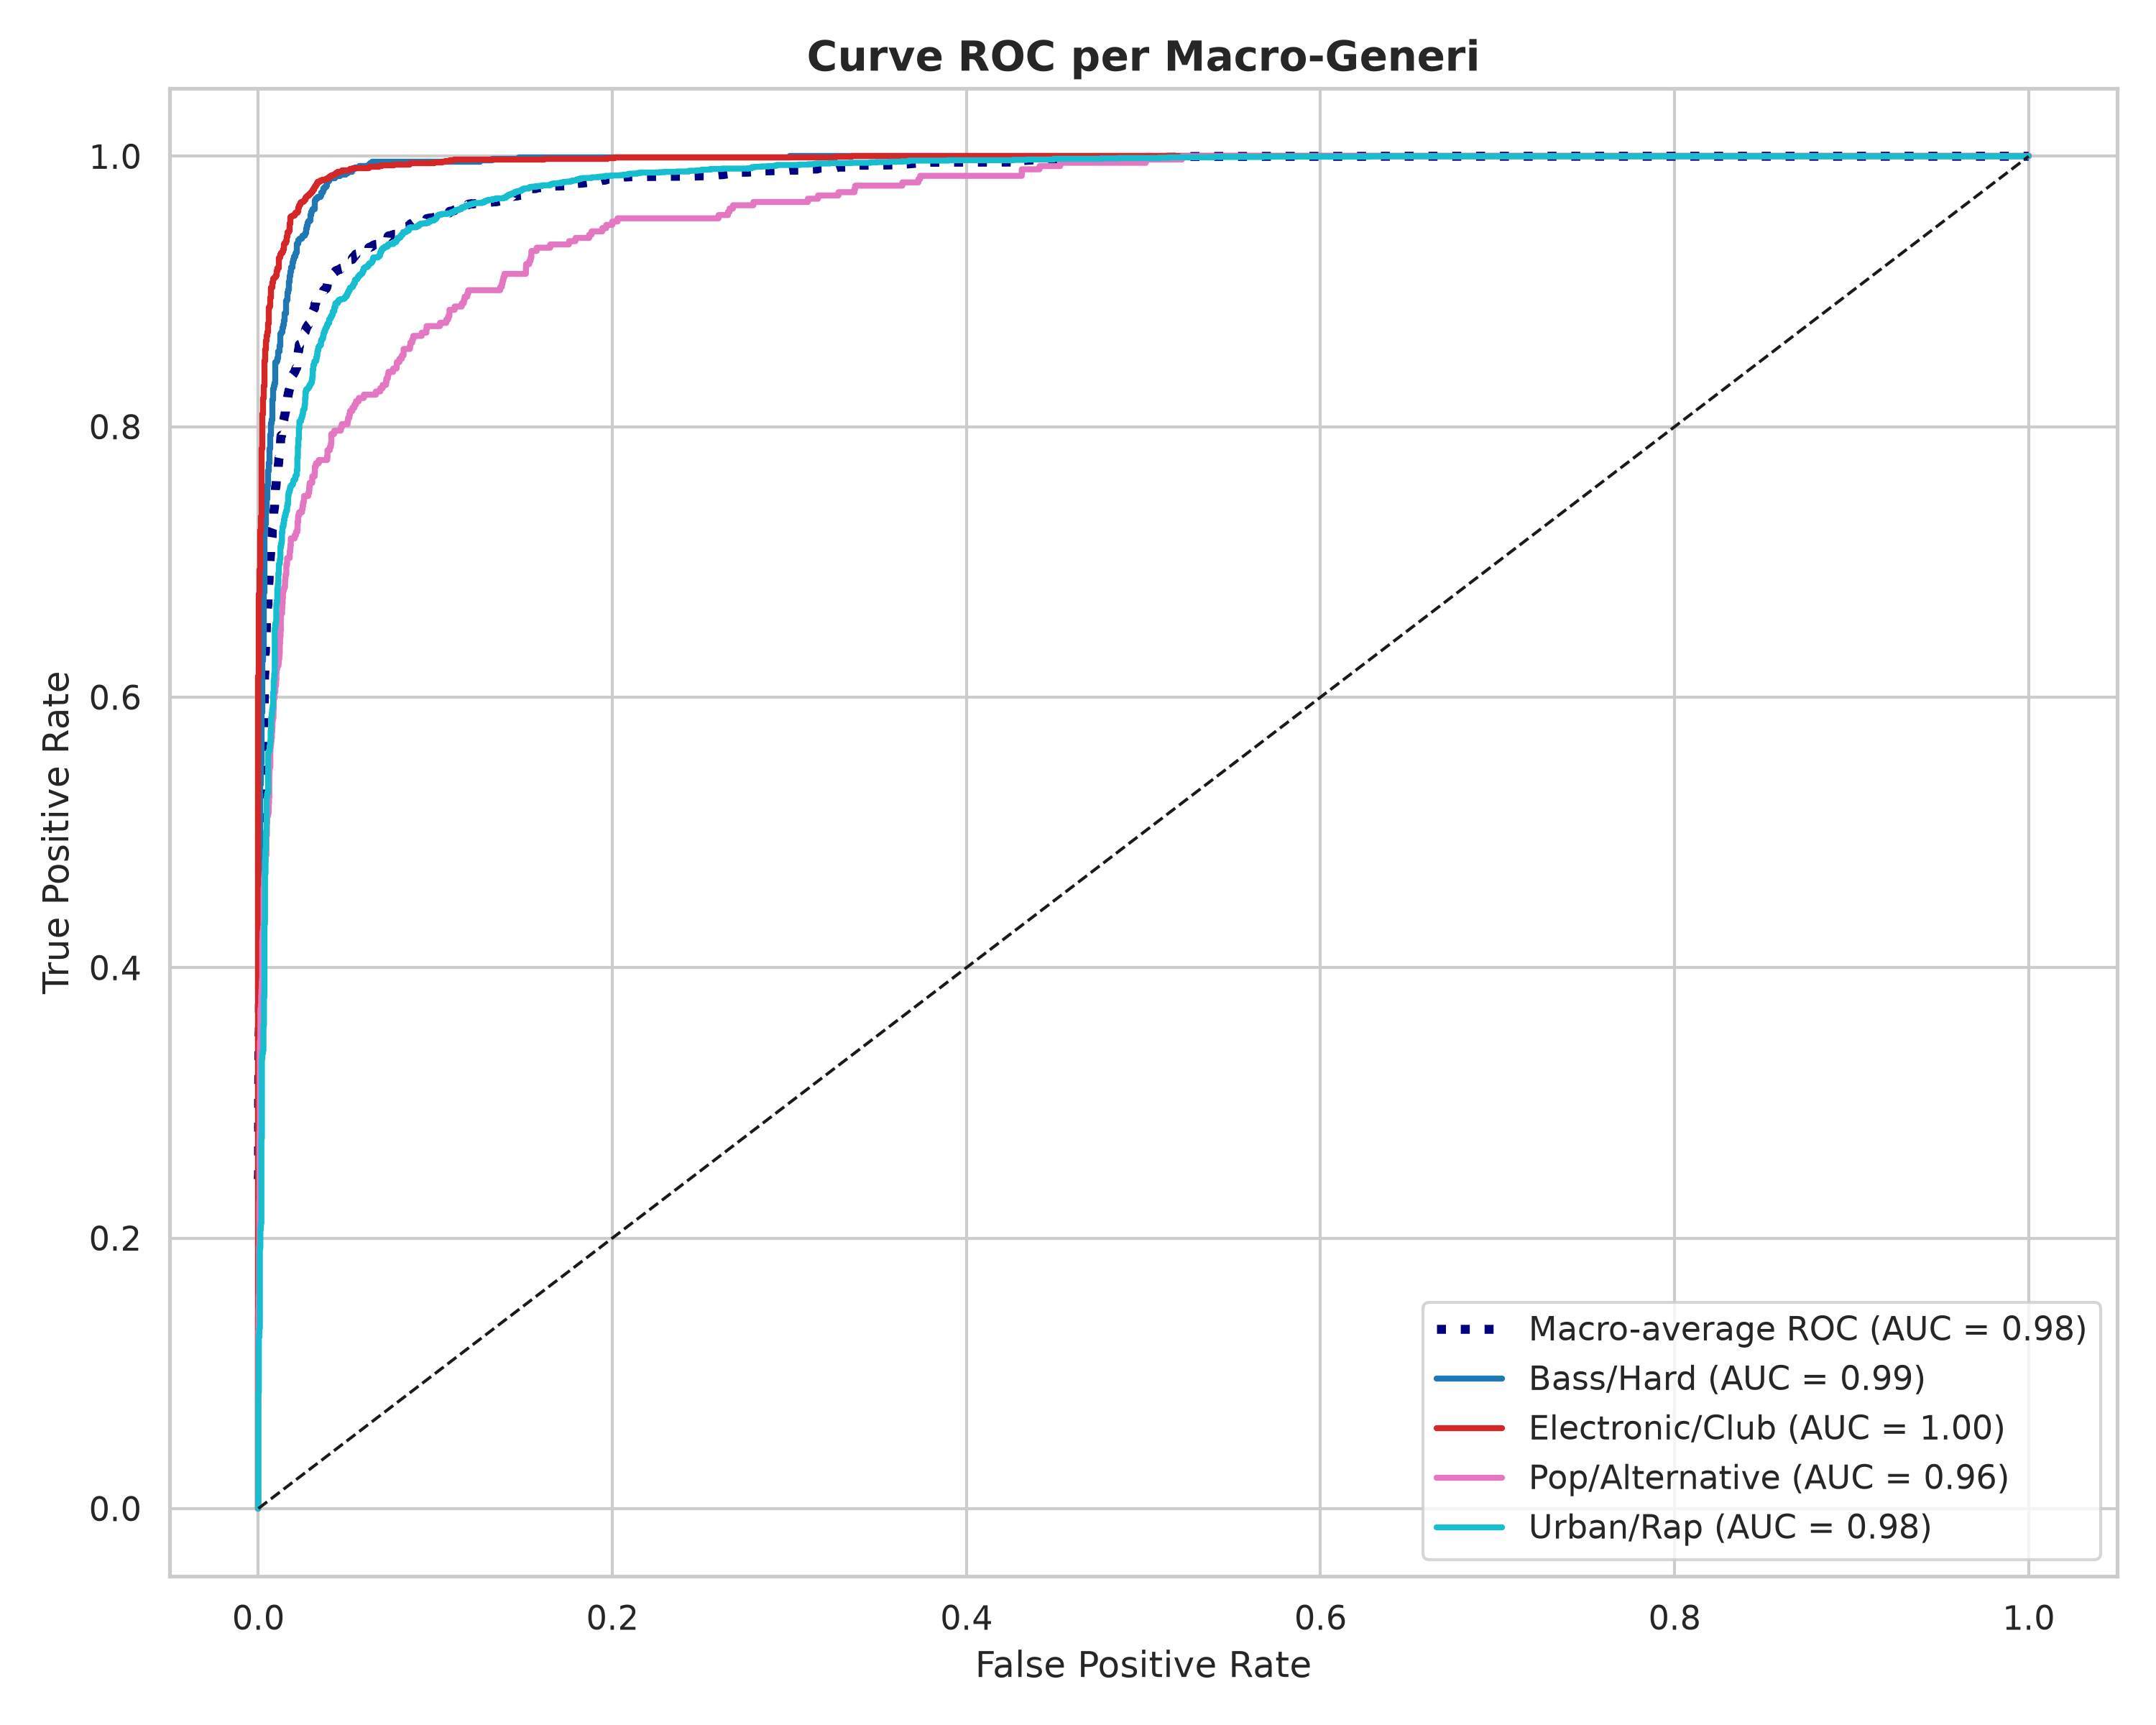
\includegraphics[width=0.78\textwidth]{figures_contu/fig10_roc_curves_macro.png}
    \caption{Curve ROC One-vs-Rest per le 4 Macro-Famiglie, con un AUC medio globale pari a 0.98 (archivio \texttt{figures\_contu/fig10\_roc_curves_macro.png}).}
    \label{fig:roc_macro}
\end{figure}

L'eccellenza discriminante al Livello 1 è pienamente corroborata dall'analisi delle curve ROC riportate in Figura \ref{fig:roc_macro}: il valore di \textbf{Macro-Average ROC-AUC raggiunge l'eccezionale quota di 0.98}. Nello specifico, la curva della famiglia \textit{Electronic/Club} converge a un AUC perfetto di \textbf{1.00}, seguita da \textit{Bass/Hard} con \textbf{0.99}, \textit{Urban/Rap} con \textbf{0.98} e \textit{Pop/Alternative} con \textbf{0.96}.

\begin{figure}[H]
    \centering
    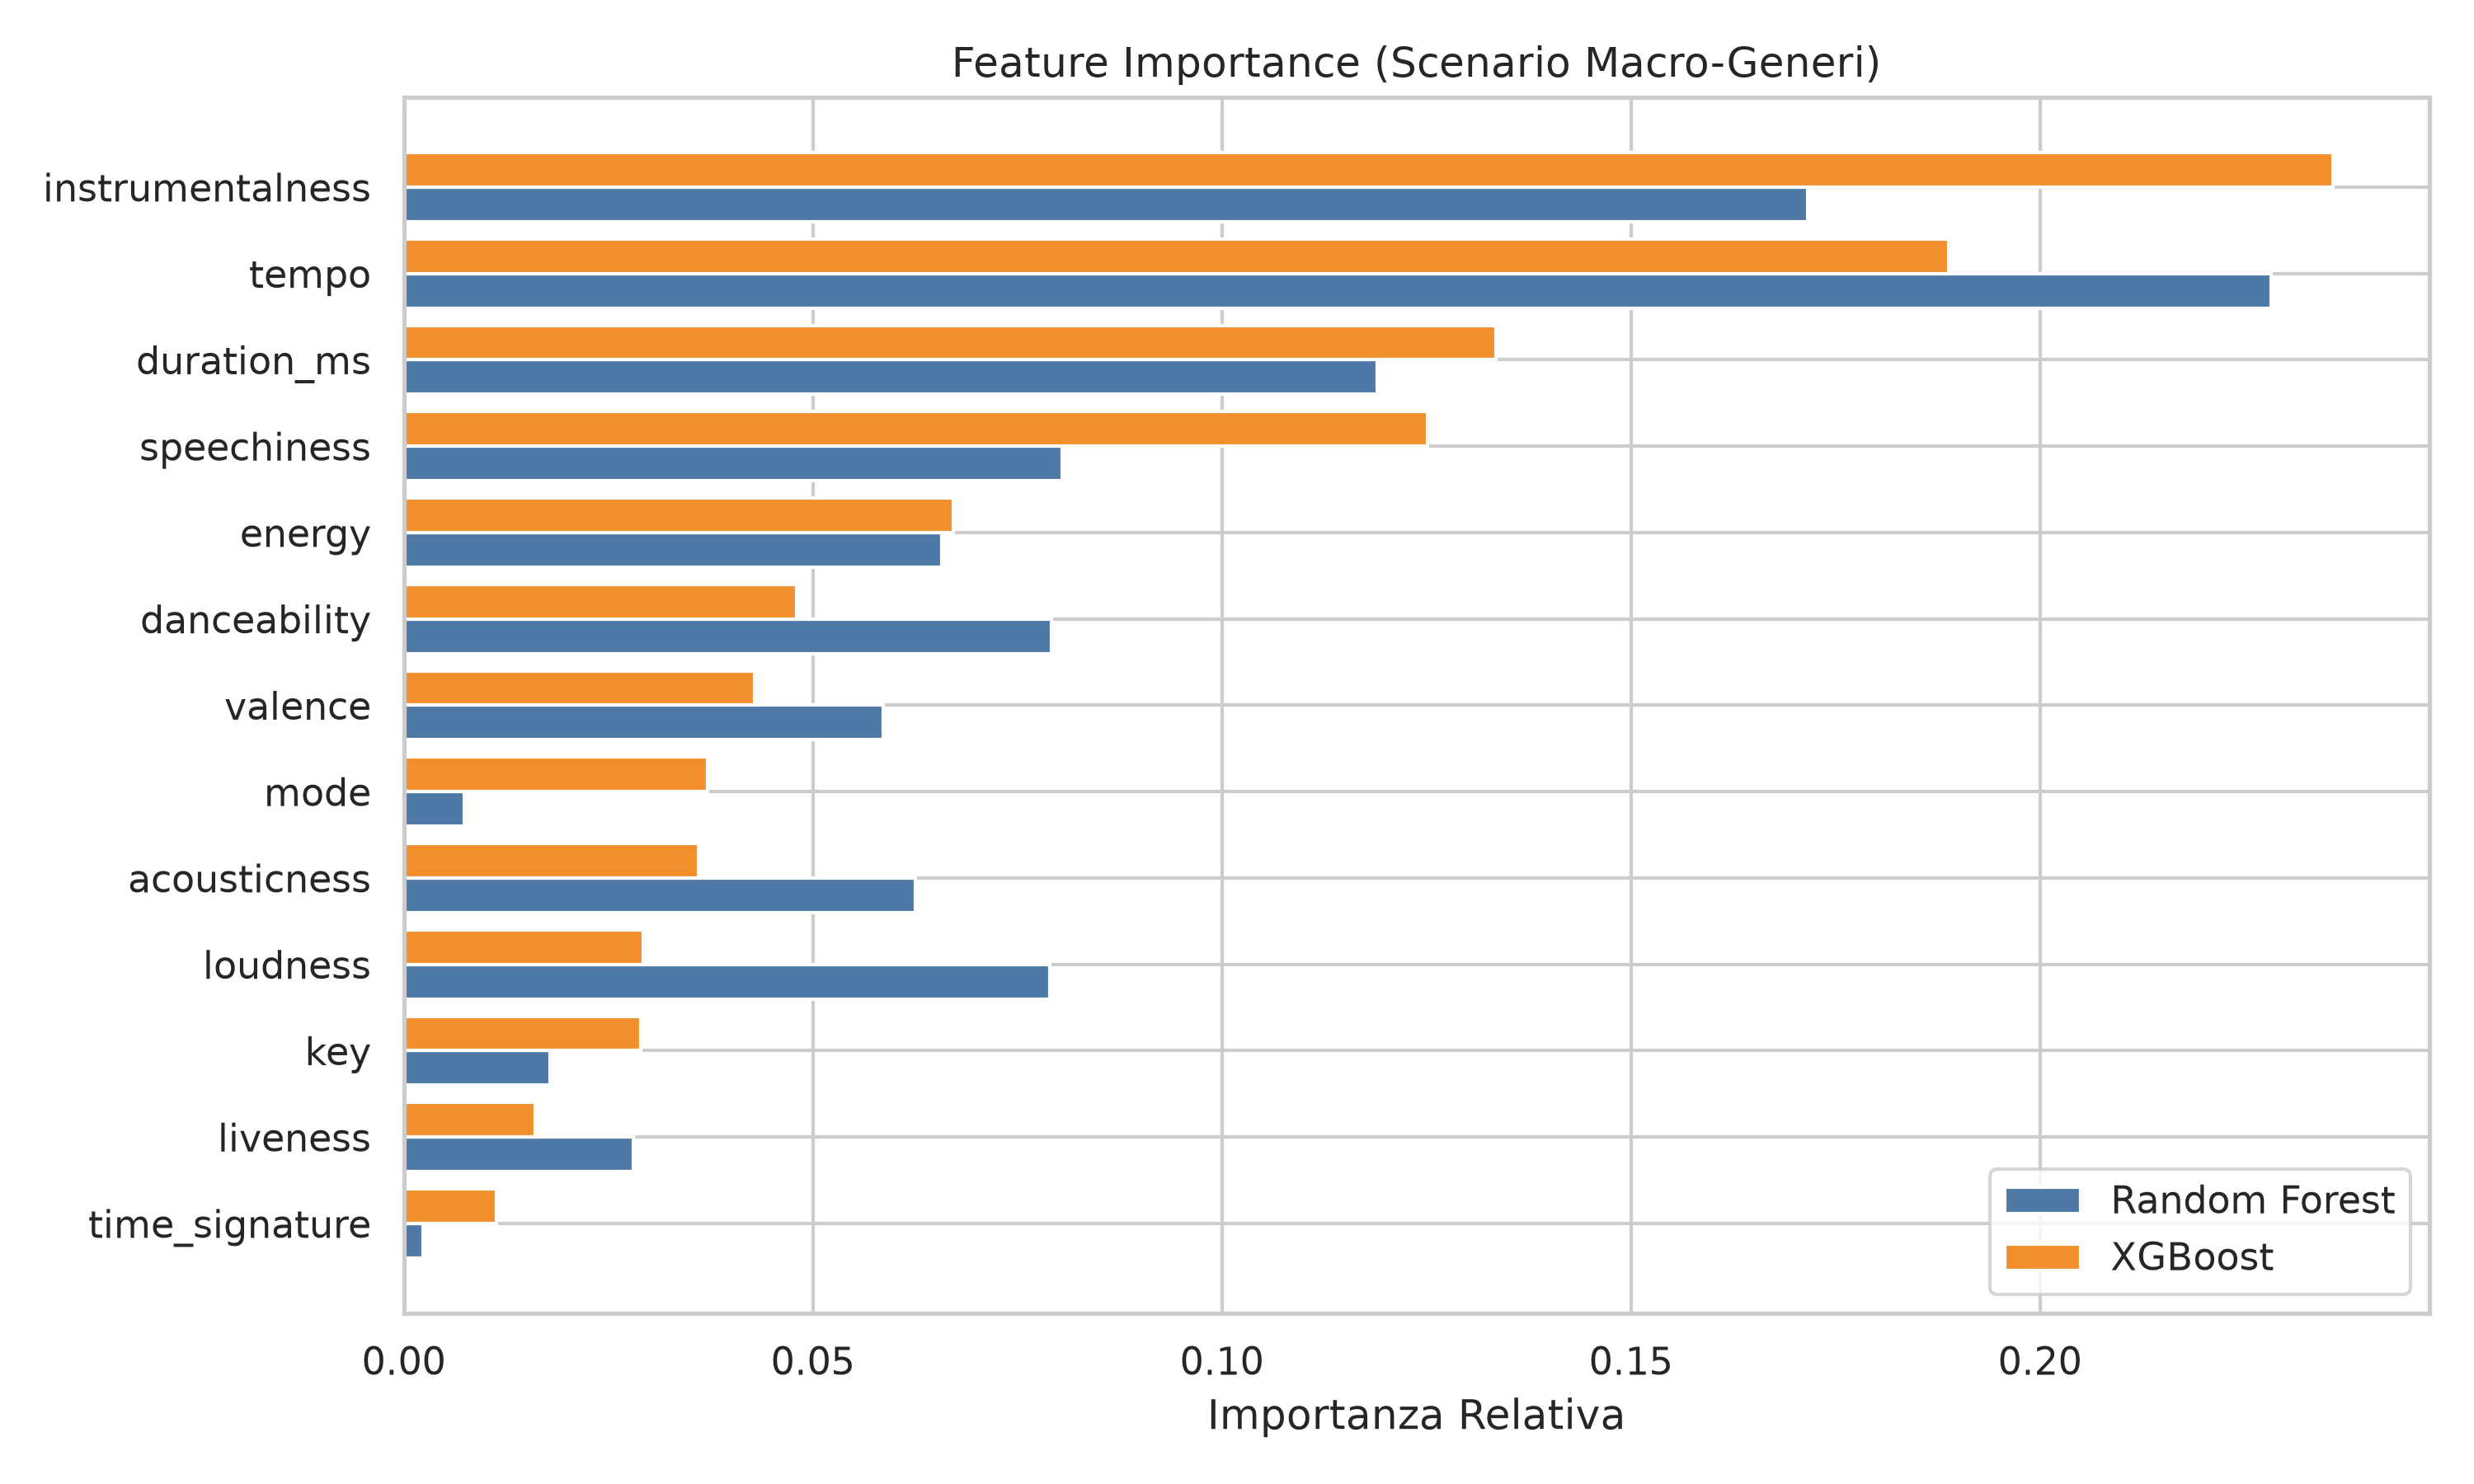
\includegraphics[width=0.85\textwidth]{figures_contu/fig13_feature_importance_macro.png}
    \caption{Importanza relativa delle feature per lo scenario a Macro-Generi calcolata da Random Forest e XGBoost (archivio \texttt{figures\_contu/fig13\_feature_importance_macro.png}).}
    \label{fig:feature_importance_macro}
\end{figure}

La ragione fisica e matematica di tale drastico incremento di performance è esplicitata dal grafico di Feature Importance di Figura \ref{fig:feature_importance_macro}. Mentre nello scenario atomico a 15 generi il modello era costretto a ricorrere quasi unicamente al fattore ritmico, a livello macro la partizione dello spazio decisionale si basa su divergenze acustiche polarizzanti e nette:
\begin{enumerate}
    \item \texttt{instrumentalness}: rappresenta in assoluto la feature cardine (contribuendo per circa il $24\%$ nel modello XGBoost e il $17\%$ in Random Forest), consentendo di discriminare istantaneamente il mondo clubbing e strumentale dalle categorie vocal-oriented;
    \item \texttt{tempo}: si conferma primario (oltre il $22\%$ per Random Forest e il $19\%$ per XGBoost), separando con nettezza le dinamiche iper-cinetiche del Bass/Hard dalle velocità cadenzate delle altre produzioni;
    \item \texttt{speechiness}: con un contributo vicino al $13\%$ in XGBoost, definisce la linea di faglia strutturale tra la metrica parlata e ritmicamente densa dell'Urban/Rap e i testi melodici o rarefatti delle altre famiglie;
    \item \texttt{duration\_ms}: concorre in modo rilevante all'isolamento delle strutture a traccia estesa tipiche dei brani da discoteca rispetto ai formati concisi dell'ascolto radiofonico e streaming.
\end{enumerate}

\newpage
\subsubsection{Livello 2: Modelli Specialisti Intra-Famiglia}

Verificata l'accuratezza dell'89.4\% nell'instradamento al macro-genere corretto, il secondo stadio della pipeline prevede l'attivazione di \textbf{4 modelli XGBoost specialisti}, ciascuno addestrato ed ottimizzato in modo dedicato all'interno dei soli campioni appartenenti a una singola macro-famiglia. L'obiettivo primario di tali modelli consiste nel verificare se, isolando il rumore generato dalle altre famiglie musicali, l'algoritmo sia in grado di cogliere pattern sottili utili a discriminare i sottogeneri interni.

Le matrici di confusione normalizzate prodotte dai quattro specialisti sul Test Set sono illustrate congiuntamente in Figura \ref{fig:specialist_confusion_matrices}.

\begin{figure}[H]
    \centering
    \begin{subfigure}[b]{0.48\textwidth}
        \centering
        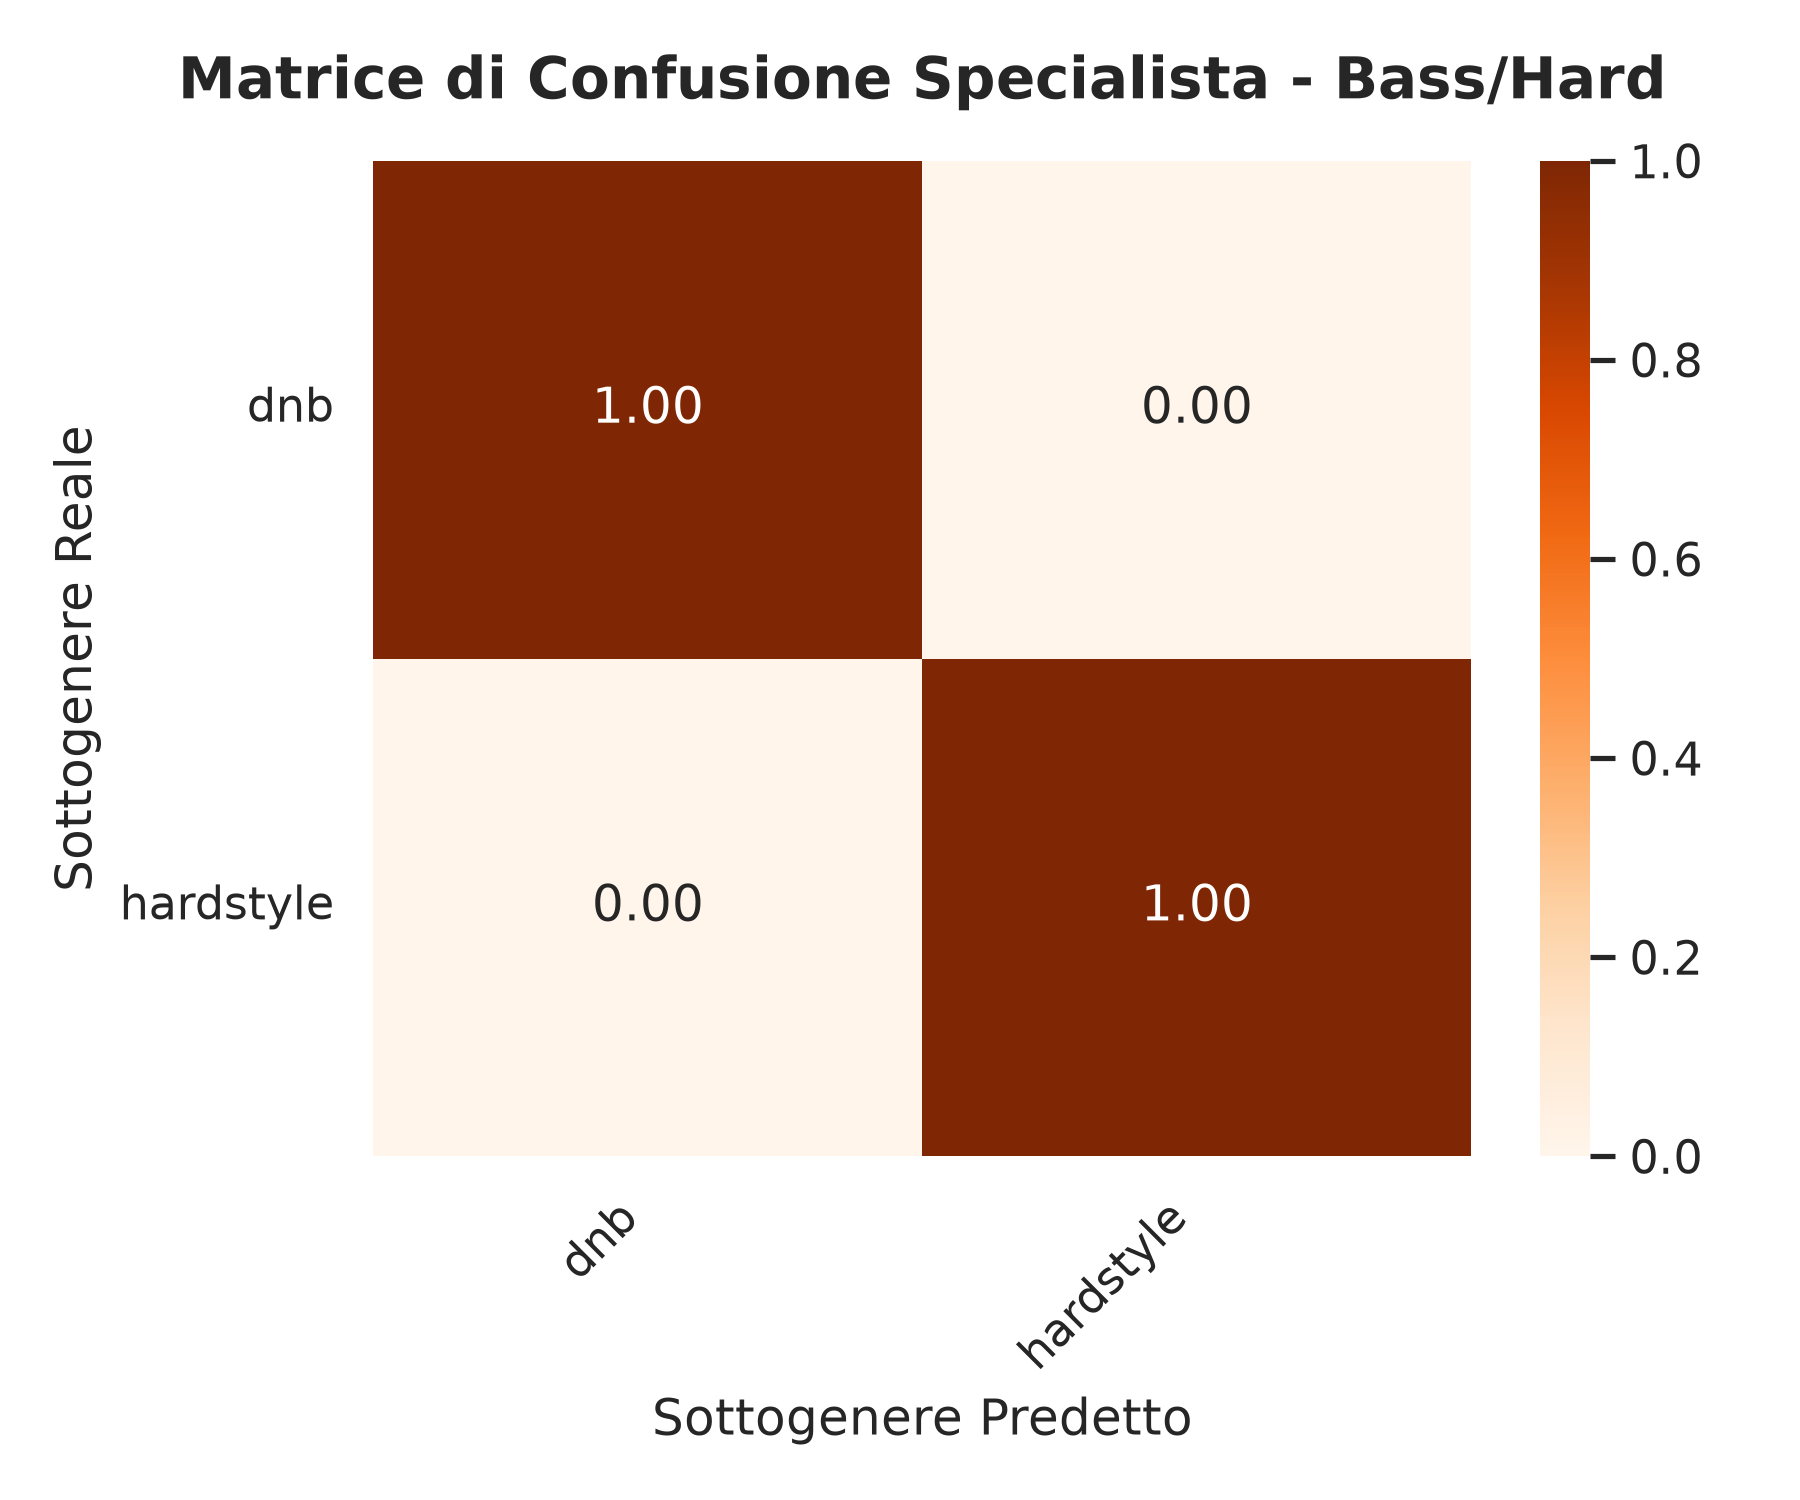
\includegraphics[width=\textwidth]{figures_contu/fig_specialist_cm_Bass_Hard.png}
        \caption{Specialista Bass/Hard (100\% di accuratezza).}
        \label{fig:sp_bass_hard}
    \end{subfigure}
    \hfill
    \begin{subfigure}[b]{0.48\textwidth}
        \centering
        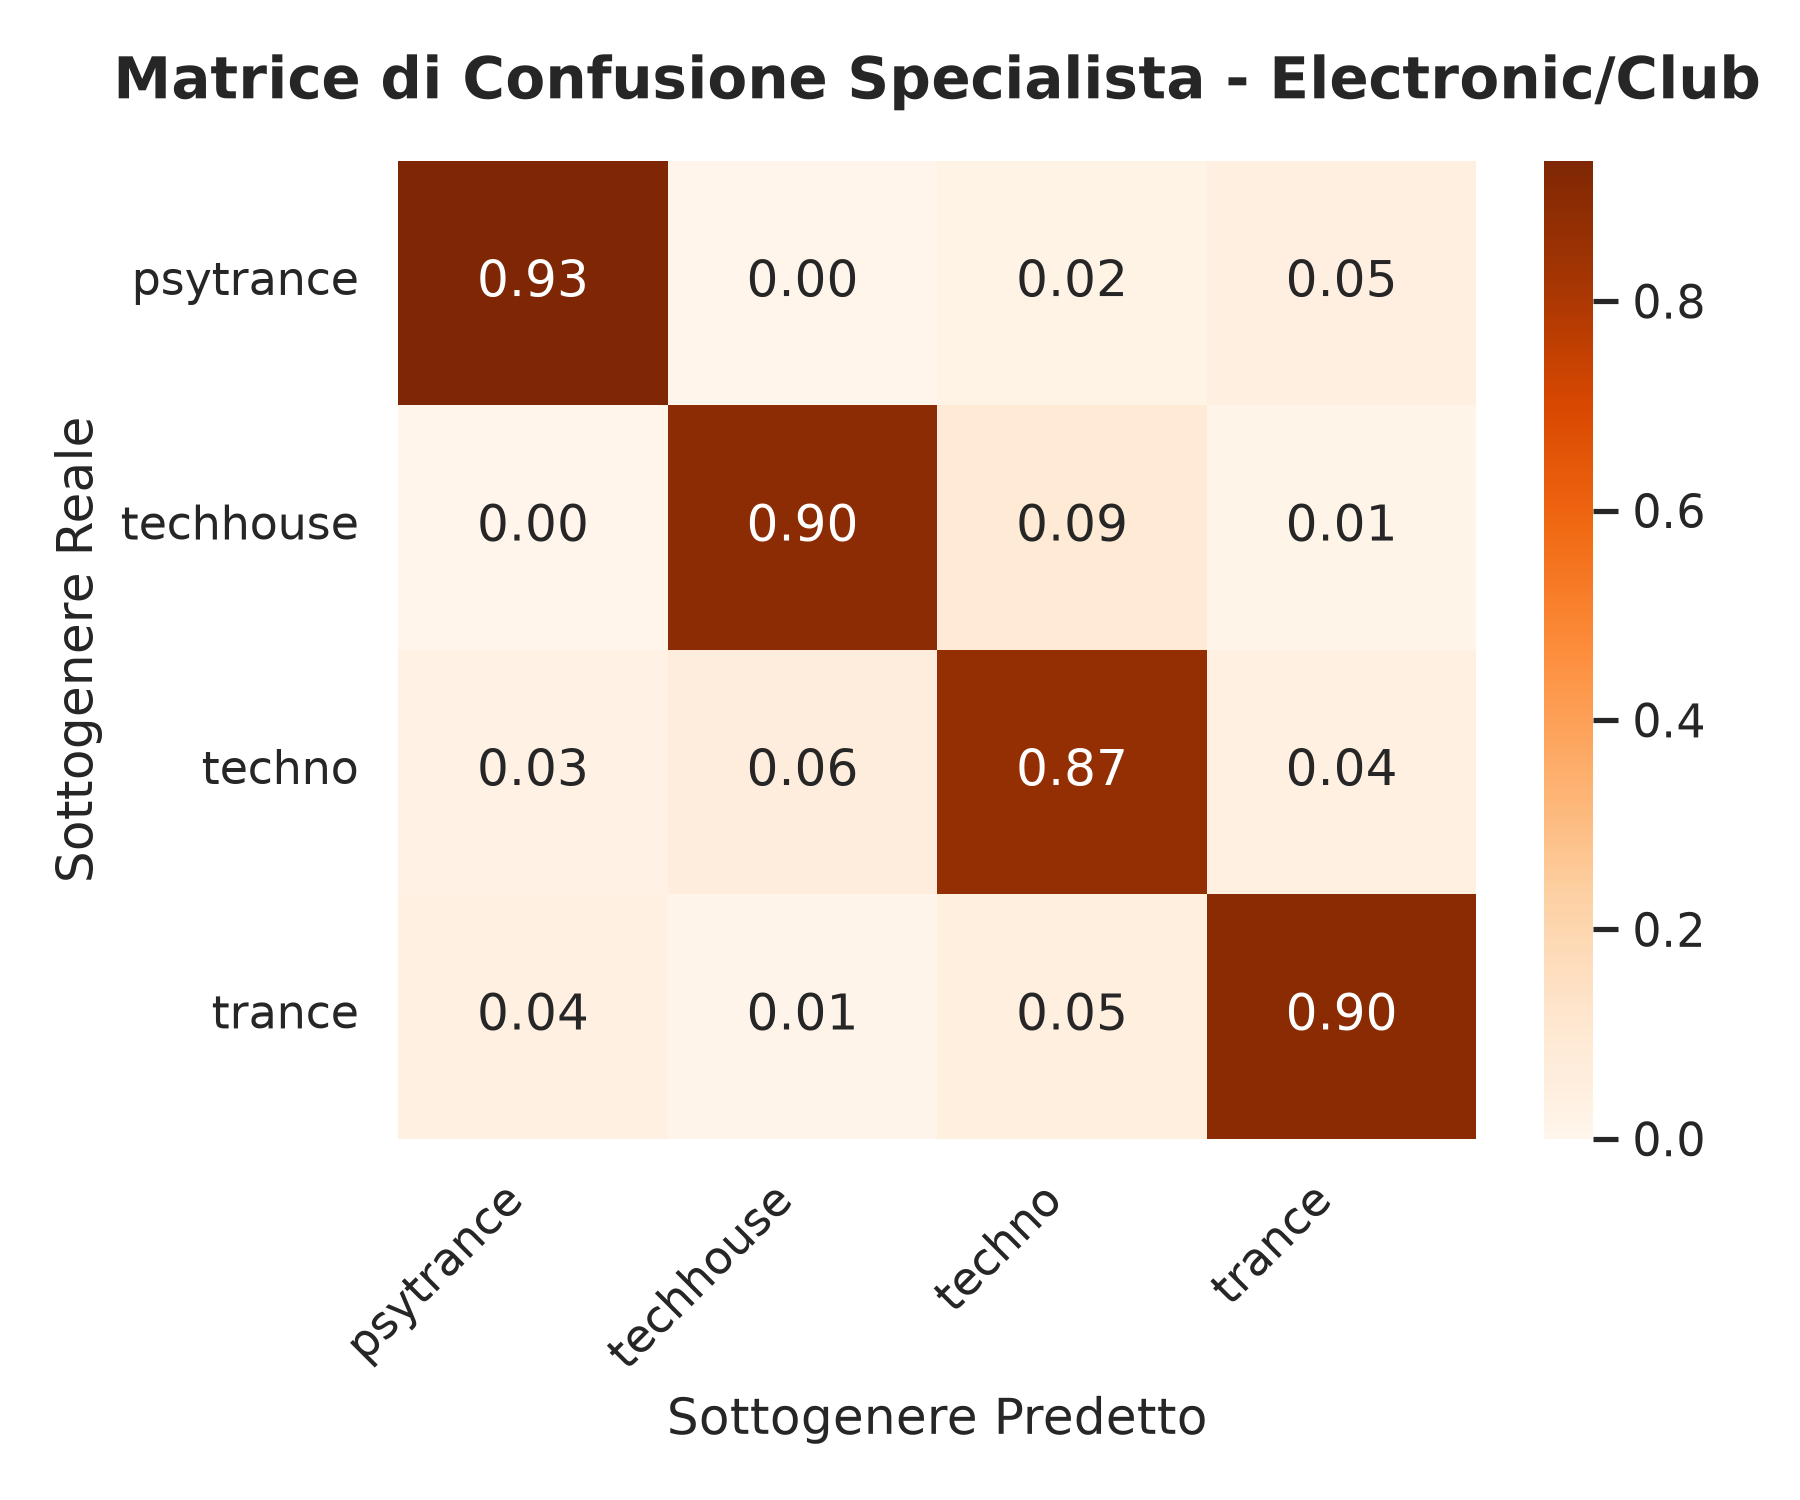
\includegraphics[width=\textwidth]{figures_contu/fig_specialist_cm_Electronic_Club.png}
        \caption{Specialista Electronic/Club (accuratezza $\ge 90\%$).}
        \label{fig:sp_electronic}
    \end{subfigure}
    \\[0.4cm]
    \begin{subfigure}[b]{0.48\textwidth}
        \centering
        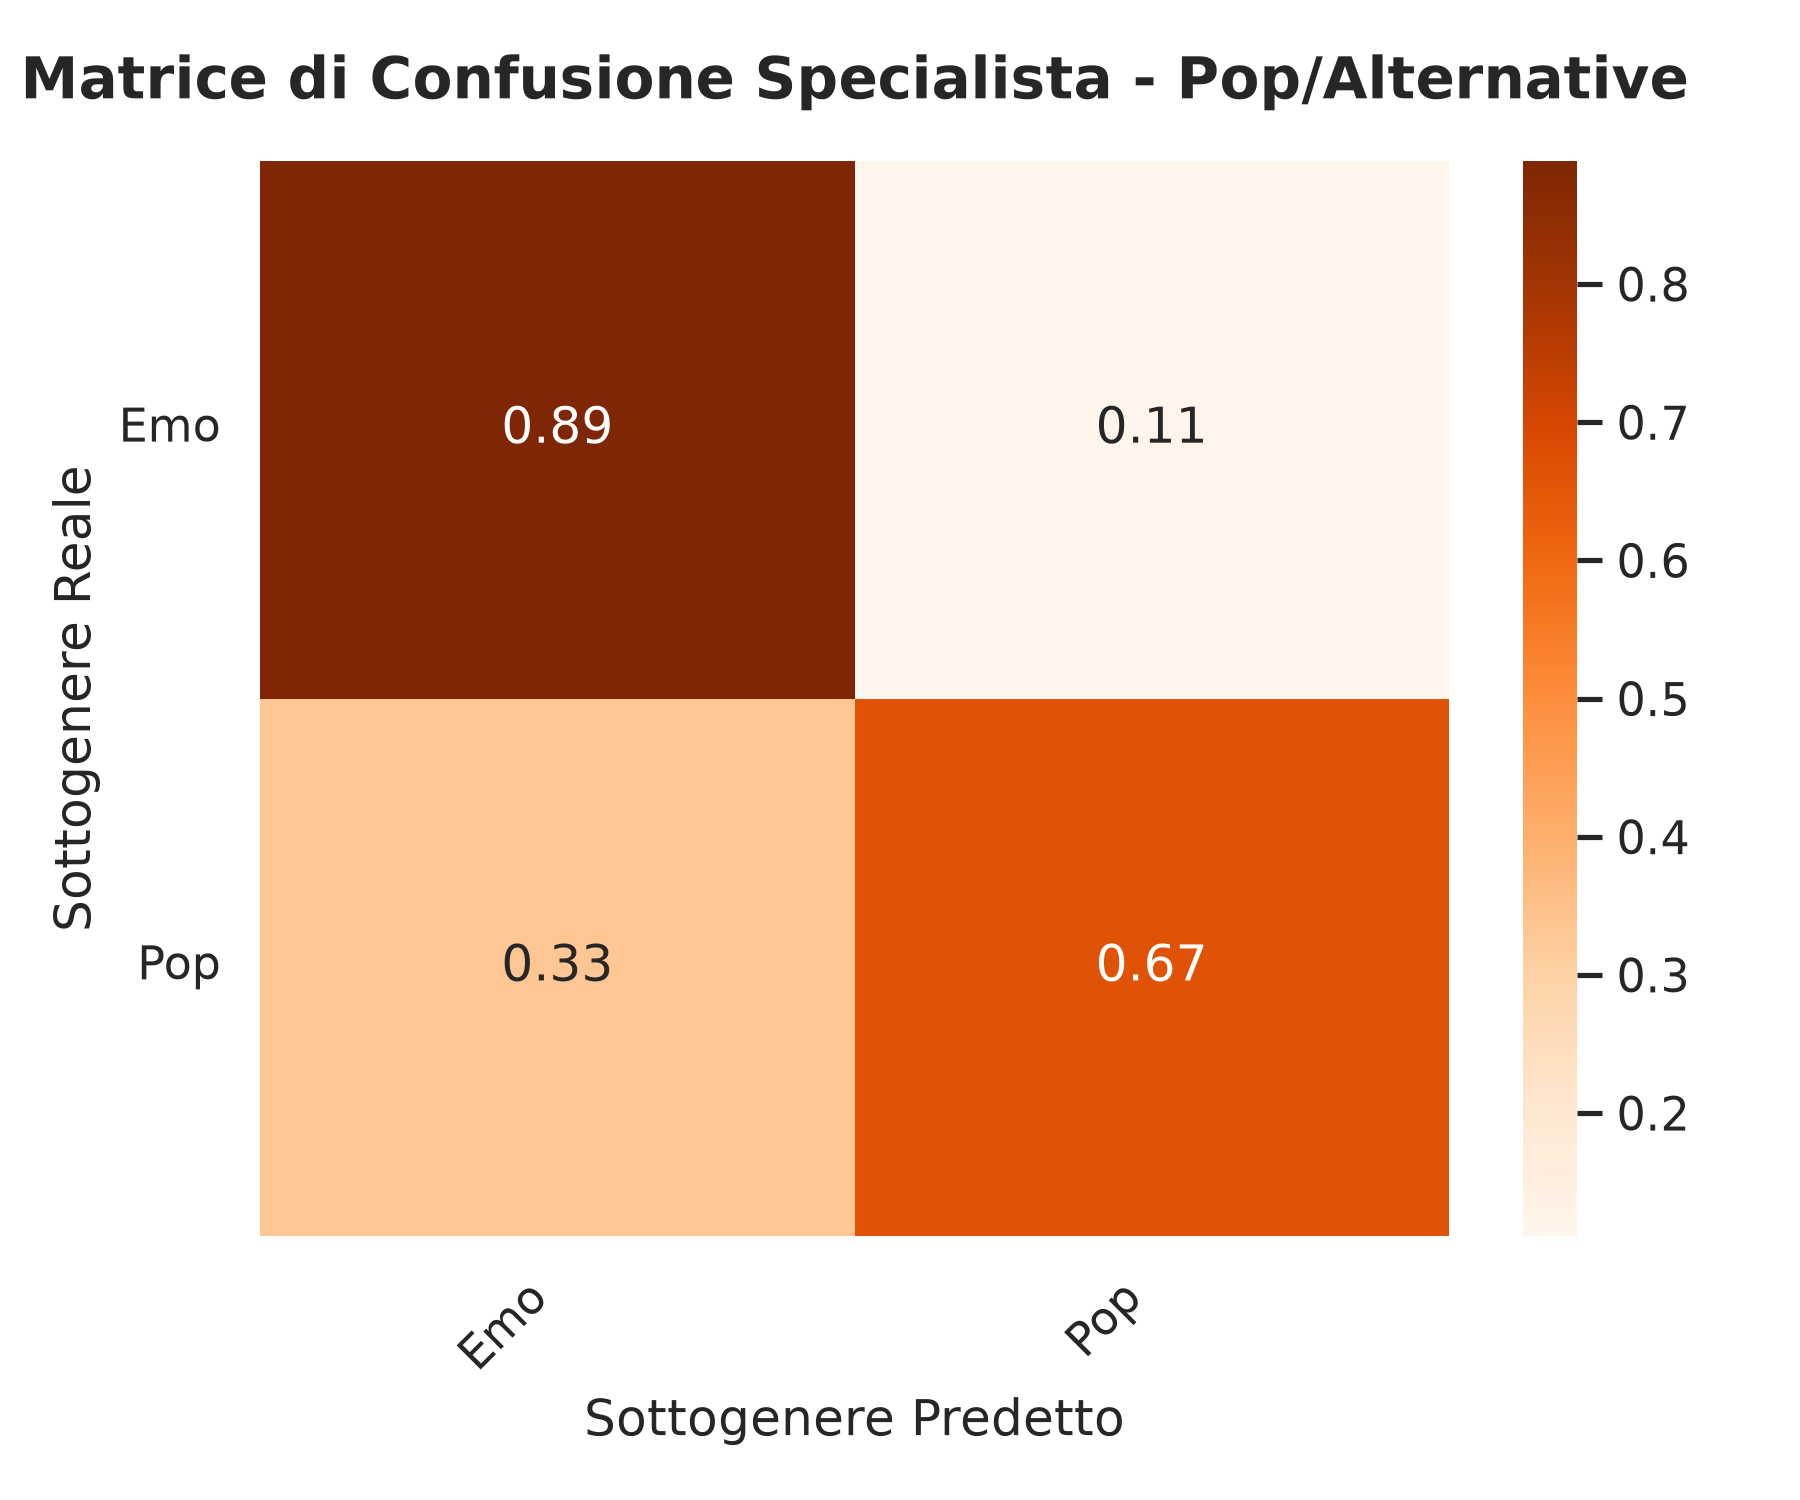
\includegraphics[width=\textwidth]{figures_contu/fig_specialist_cm_Pop_Alternative.png}
        \caption{Specialista Pop/Alternative (Emo vs Pop).}
        \label{fig:sp_pop_alt}
    \end{subfigure}
    \hfill
    \begin{subfigure}[b]{0.48\textwidth}
        \centering
        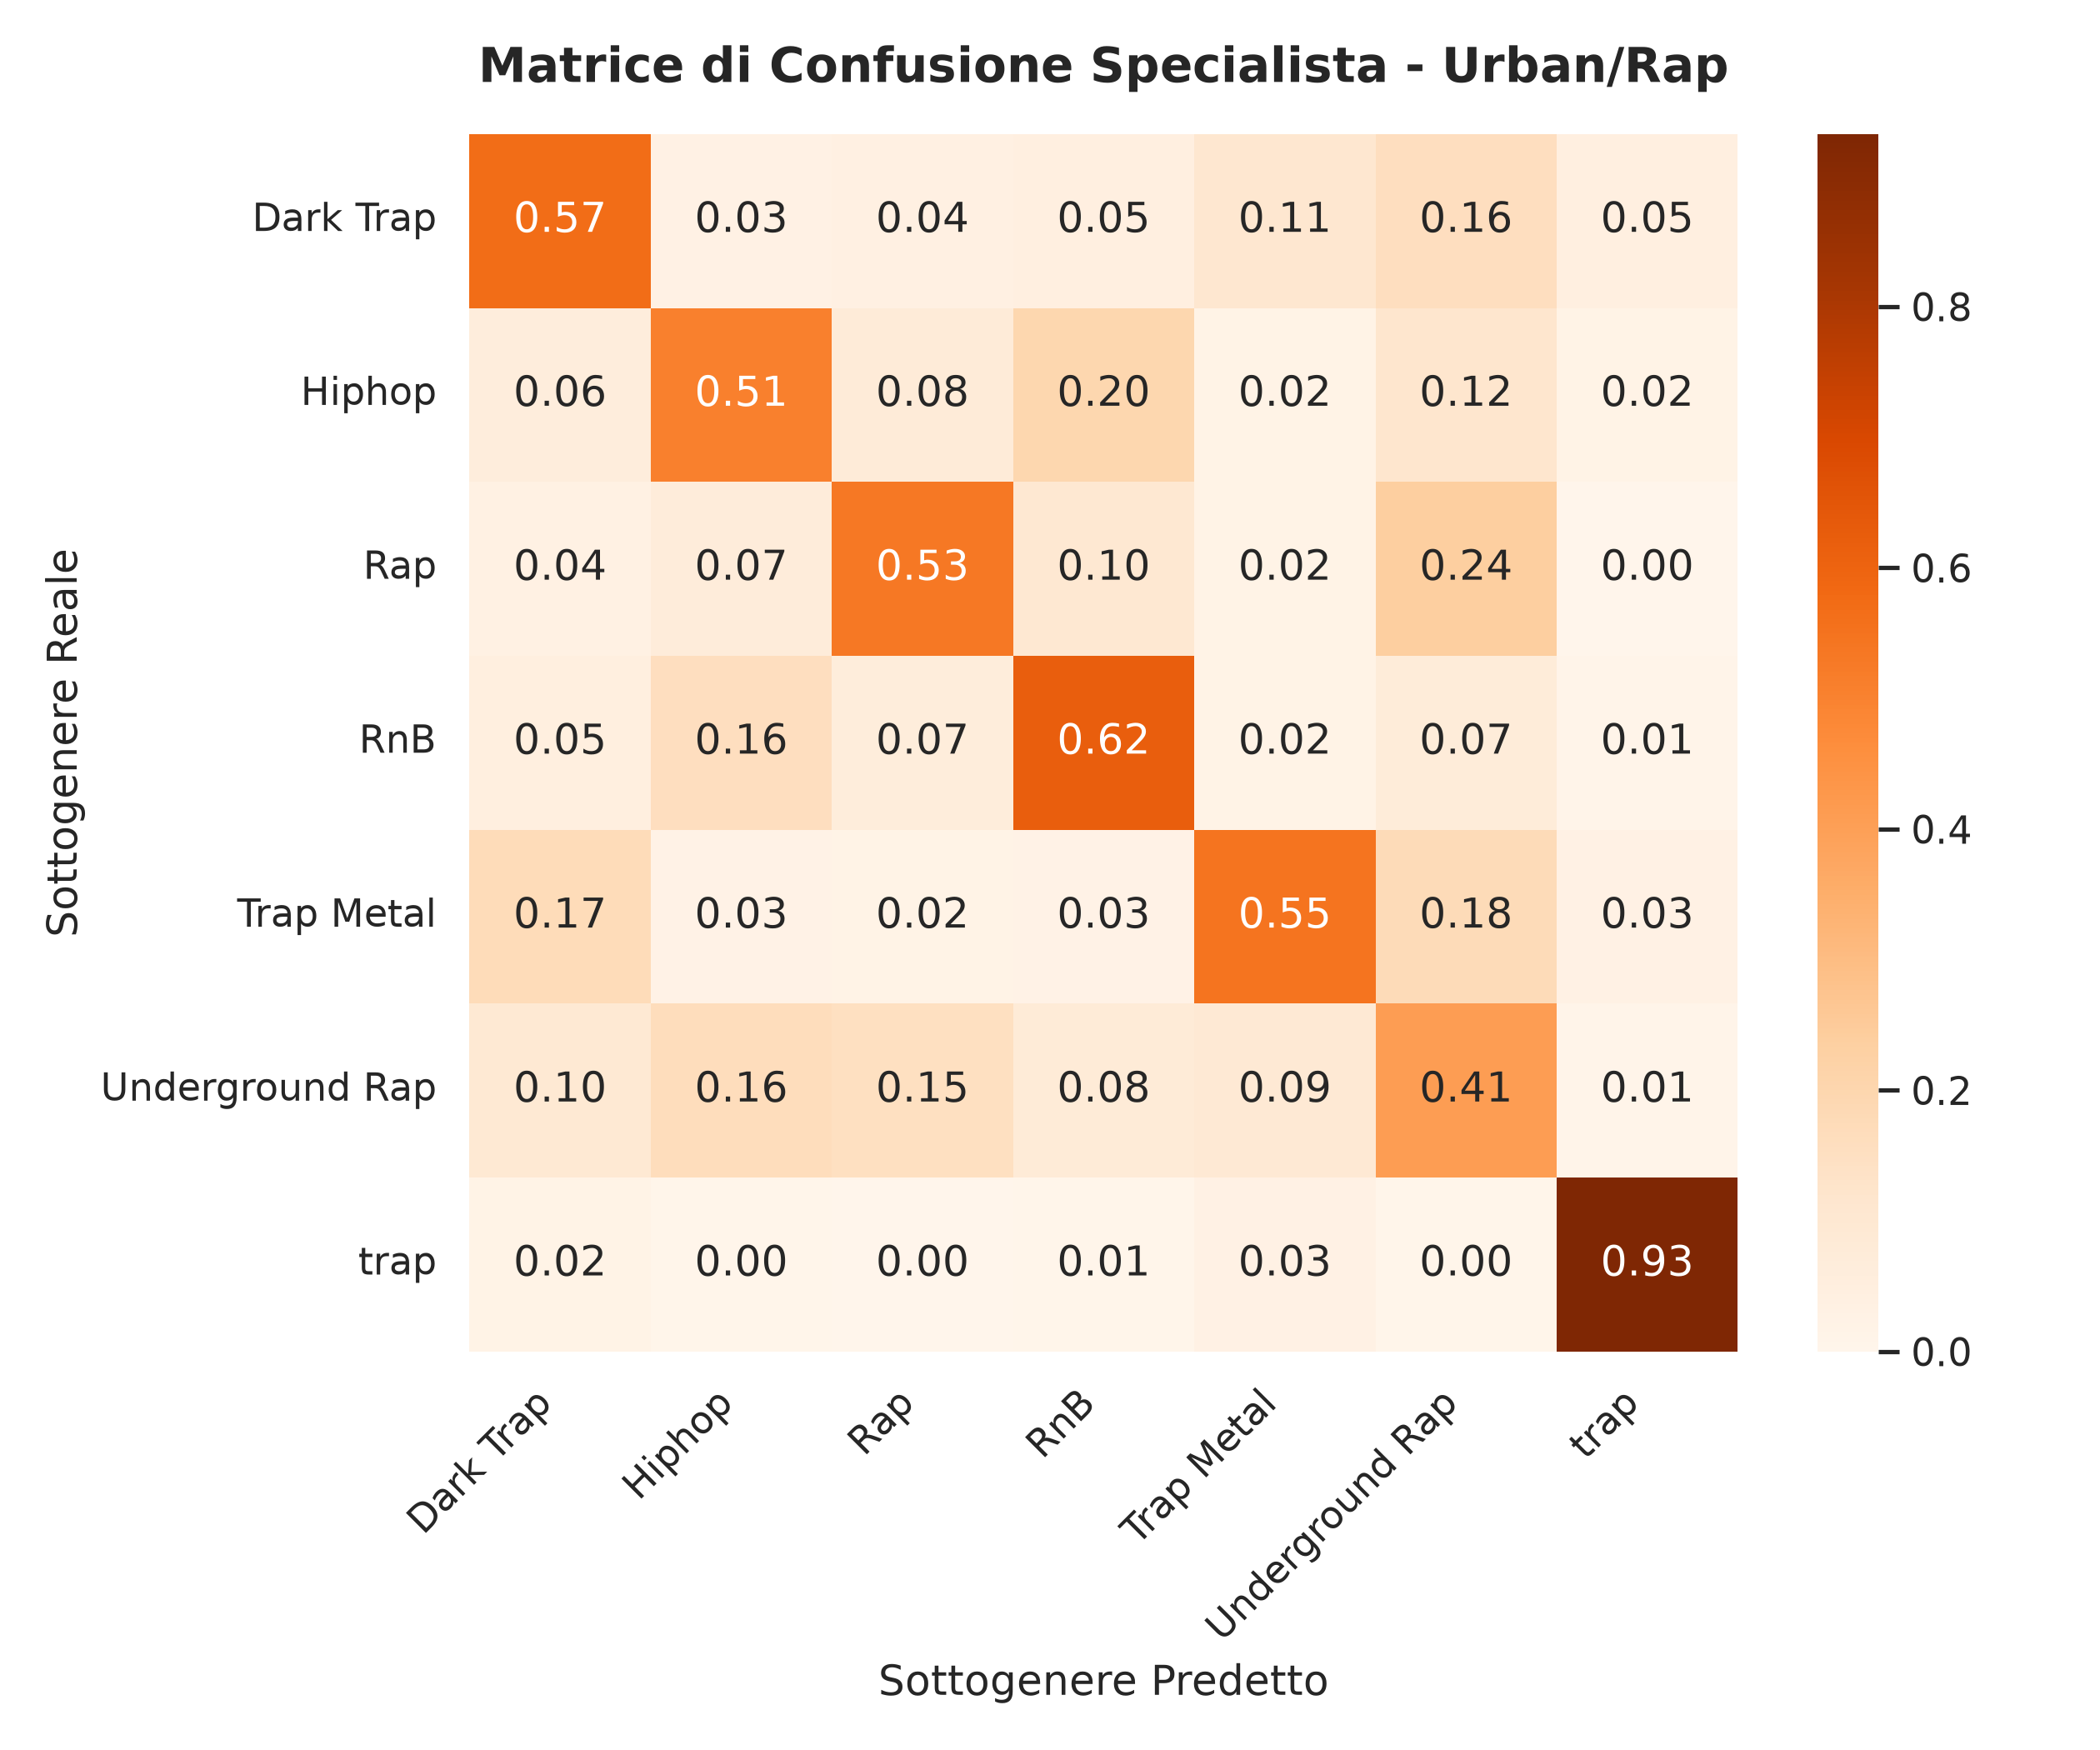
\includegraphics[width=\textwidth]{figures_contu/fig_specialist_cm_Urban_Rap.png}
        \caption{Specialista Urban/Rap (evidente overlap acustico).}
        \label{fig:sp_urban_rap}
    \end{subfigure}
    \caption{Matrici di confusione dei 4 classificatori specialisti XGBoost di Livello 2 addestrati sulle singole macro-famiglie (file della suite \texttt{figures\_contu}).}
    \label{fig:specialist_confusion_matrices}
\end{figure}

Dall'analisi comparativa dei quattro modelli emergono comportamenti profondamente divergenti a seconda della natura intrinseca del genere musicale:
\begin{itemize}
    \item \textbf{Specialista Bass/Hard (Figura \ref{fig:sp_bass_hard}):} Raggiunge un risultato teoricamente e operativamente impeccabile, registrando il \textbf{100\% esatto di accuratezza} su entrambi i sottogeneri (\textit{dnb} = 1.00, \textit{hardstyle} = 1.00) con zero campioni confusi. La netta divergenza tra la ritmica breakbeat a 174 BPM della Drum and Bass e la cassa quadrupla a 150 BPM con saturazione armonica dell'Hardstyle permette allo specialista una separazione perfetta nello spazio delle caratteristiche audio.
    \item \textbf{Specialista Electronic/Club (Figura \ref{fig:sp_electronic}):} Evidenzia una capacità discriminante eccellente, attestandosi costantemente su percentuali attorno o superiori al 90\% di classificazione corretta: \textit{psytrance} al \textbf{93\%}, \textit{techhouse} al \textbf{90\%}, \textit{trance} al \textbf{90\%} e \textit{techno} all'\textbf{87\%}. Le uniche lievi confusioni si manifestano tra \textit{techno} e \textit{techhouse} ($6\%$ e $9\%$), dovute alla comune impostazione 4/4 a battute contigue ($\approx 125-130$ BPM).
    \item \textbf{Specialista Pop/Alternative (Figura \ref{fig:sp_pop_alt}):} Mostra una separazione asimmetrica: mentre la classe \textit{Emo} viene isolata con una solida accuratezza dell'\textbf{89\%}, ben il \textbf{33\% delle tracce etichettate come Pop viene erroneamente attribuito all'Emo} (con il Pop corretto ad appena il 67\%). Tale fenomeno riflette la marcata convergenza stilistica del pop moderno con chitarre acustiche e distorte ed atmosfere malinconiche tipiche del filone emo/alternative.
    \item \textbf{Specialista Urban/Rap (Figura \ref{fig:sp_urban_rap}):} In netto contrasto con i successi degli altri specialisti, all'interno del comparto urbano l'accuratezza subisce un vero e proprio tracollo:
    \begin{itemize}
        \item \textit{Underground Rap} viene riconosciuto correttamente soltanto nel \textbf{41\%} dei casi, disperdendosi in maniera generalizzata verso Rap ($15\%$), Hiphop ($16\%$), Dark Trap ($10\%$) e Trap Metal ($9\%$);
        \item \textit{Rap} registra un'accuratezza di appena il \textbf{53\%}, con il $24\%$ delle proprie osservazioni scambiate per Underground Rap e il $10\%$ per RnB;
        \item \textit{Hiphop} viene predetto con successo solo nel \textbf{51\%} dei casi, mostrando una dispersione critica verso RnB ($20\%$) e Underground Rap ($12\%$);
        \item \textit{Trap Metal} ($55\%$) e \textit{Dark Trap} ($57\%$) evidenziano confusioni incrociate biunivoche con il resto del bacino rap;
        \item L'unica eccezione rilevante è costituita dalla classe \textit{trap} (con un'accuratezza del \textbf{93\%}), la cui tipica ritmica cadenzata con sub-bassi 808 scivolati e triplette di hi-hat a frequenza caratteristica ne preserva la riconoscibilità rispetto al rap classico.
    \end{itemize}
\end{itemize}

\subsubsection{Conclusione Diagnostica e Considerazioni sulla Natura delle Etichette}

La sperimentazione gerarchica condotta conduce a una conclusione diagnostica di fondamentale valore metodologico ed epistemologico per l'intero lavoro di tesi:
\begin{quote}
\textit{L'approccio a cascata a due stadi dimostra inconfutabilmente che l'apparato algoritmico e le tecniche di Machine Learning impiegate sono estremamente validi ed efficaci.}
\end{quote}

Nel momento in cui nel segnale acustico sono presenti differenze timbriche, spettrali e ritmiche oggettive, i modelli di classificazione raggiungono vette di accuratezza prossime o uguali alla perfezione (l'89.4\% a livello macro, con punte del 97\% nell'Electronic e il 100\% nel Bass/Hard).

Alla luce di questa constatazione, il drastico crollo delle performance riscontrato nello specialista \textit{Urban/Rap} non può e non deve essere interpretato come un limite matematico dei modelli predittivi, né come una carenza nel processo di tuning degli iperparametri o nella formulazione del training set. Al contrario, tale esito costituisce la \textbf{formale dimostrazione empirica che i sottogeneri del macro-universo Urban/Rap condividono la medesima, identica impronta e firma acustica}.

Dal punto di vista dell'elaborazione del segnale e dell'estrazione delle caratteristiche sonore (BPM, danceability, energy, loudness, tempo e valence), una traccia classificata da Spotify come \textit{Rap}, \textit{Hiphop} o \textit{Underground Rap} non possiede alcuna differenziazione fisico-armonica misurabile. Le etichette attribuite dalla piattaforma per questa specifica famiglia non riflettono caratteristiche acustiche oggettive, bensì possiedono una valenza prettamente \textbf{culturale, sociologica, contestuale e di marketing editoriale}:
\begin{itemize}
    \item La qualifica di \textit{Underground} rispetto a \textit{Rap} commerciale è determinata dal canale di distribuzione indipendente, dalla notorietà dell'artista e dal target del pubblico, non dal timbro della base musicale;
    \item La demarcazione tematica tra \textit{Dark Trap}, \textit{Trap Metal} o \textit{Hiphop} convenzionale risiede prevalentemente nel contenuto semantico dei testi, nel messaggio sociopolitico e nella crudezza verbale delle rime.
\end{itemize}

Poiché il dataset impiegato è circoscritto alle sole feature ingegneristiche fornite dalle Web API di Spotify e prescinde totalmente dall'analisi del testo (\textit{Natural Language Processing} sulle liriche), il modello si scontra con una frontiera di Bayes intrinsecamente invalicabile: \textbf{non è possibile separare matematicamente ciò che a livello sonoro risulta perfettamente identico}. Tale constatazione sigilla il capitolo con una chiara linea di demarcazione tra ciò che è estraibile dal puro segnale acustico e ciò che appartiene indissolubilmente alla sfera semantico-culturale della musica moderna.


\newpage
% CAPITOLO 4: CLUSTERING
% =========================================================================
\section{Spotify tracks analysis: clustering}

Questo capitolo ha lo scopo di illustrare l'applicazione di tecniche di clusterizzazione non supervisionata con l'obiettivo di suddividere il dataset in gruppi o cluster caratterizzati da proprietà acustiche simili, operando in modo del tutto agnostico rispetto alle etichette di genere commerciale e rimuovendo la colonna target \texttt{genre}.

In generale, le tecniche di clustering si suddividono in diverse famiglie metodologiche:
\begin{itemize}
    \item \textbf{Clusterizzazione per partizione:} Suddivide i dati in $k$ cluster predefiniti, ottimizzando una funzione obiettivo (come la minimizzazione della distanza intra-cluster e la massimizzazione della distanza inter-cluster).
    \item \textbf{Clusterizzazione basata su densità:} Identifica i cluster come regioni densamente popolate nello spazio dati, separate da aree a bassa densità, isolando autonomamente i punti anomali come rumore.
    \item \textbf{Clusterizzazione gerarchica:} Costruisce un albero di raggruppamento (dendrogramma) combinando iterativamente i campioni più vicini o dividendo i gruppi esistenti.
    \item \textbf{Clusterizzazione basata su modello:} Assume che i dati siano generati da una combinazione di distribuzioni statistiche sottostanti (ad esempio Gaussian Mixture Models).
\end{itemize}

Gli algoritmi confrontati comprendono K-Means (partizionamento), GMM (modello di mistura probabilistico) e DBSCAN/HDBSCAN (clustering basato su densità). GMM e HDBSCAN estendono rispettivamente le analisi iniziali con appartenenze probabilistiche e una gestione gerarchica delle densità.

\subsection{Fase di ETL per il clustering}

\subsubsection{Operazioni preliminari e selezione delle feature}

Prima di applicare gli algoritmi di clustering, il dataset deduplicato ($N = 35.877$ brani) è stato sottoposto a un processo mirato di selezione e trasformazione delle variabili, indispensabile per garantire che la distanza euclidea rifletta reali affinità timbriche, ritmiche ed emotive:
\begin{itemize}
    \item \textbf{Eliminazione della variabile target \texttt{genre} e dei metadati identificativi:} La colonna commerciale \texttt{genre} e gli attributi di servizio (\texttt{id}, \texttt{uri}, ecc.) sono stati esclusi per assicurare un apprendimento rigorosamente non supervisionato.
    \item \textbf{Selezione delle Feature Continue e Prevenzione delle Distorsioni Metriche:} A differenza degli alberi decisionali impiegati nella classificazione supervisionata (che operano tramite soglie ortogonali indipendenti dalla scala), gli algoritmi basati su distanza euclidea come K-Means e DBSCAN soffrono severamente in presenza di variabili discrete codificate come interi, variabili ridondanti o attributi contestuali. Partendo dalle 13 feature originarie, sono state quindi escluse 5 variabili:
    \begin{enumerate}
        \item Le 3 variabili discrete/categoriche di notazione musicale (\texttt{key}, \texttt{mode}, \texttt{time\_signature}), poiché la loro natura ciclica o binaria introduce salti artificiali nella geometria euclidea (ad esempio, la tonalità \texttt{key=0} [Do] e \texttt{key=11} [Si] sono adiacenti nel circolo cromatico ma risulterebbero agli antipodi metrici).
        \item La variabile \texttt{loudness}, in quanto fortemente collineare con \texttt{energy} ($r = 0,70$, come evidenziato nella matrice di correlazione di Figura \ref{fig:matrice_corr_iniziale}): mantenerle entrambe duplicherebbe impropriamente il peso dell'intensità sonora nella determinazione dei centroidi.
        \item La variabile \texttt{liveness}, poiché misura la probabilità che la traccia sia stata registrata dal vivo in presenza di pubblico (contesto di esecuzione) e non una proprietà musicale o emotiva intrinseca del brano.
    \end{enumerate}
    Il sottoinsieme finale per il clustering comprende pertanto le \textbf{8 feature acustiche continue fondamentali}: \texttt{danceability}, \texttt{energy}, \texttt{speechiness}, \texttt{acousticness}, \texttt{instrumentalness}, \texttt{valence}, \texttt{tempo} e \texttt{duration\_ms}.
    \item \textbf{Standardizzazione Statistica Obbligatoria (Z-score) e Rischio di Dominanza della Varianza:} Prima di applicare la PCA e gli algoritmi basati su distanza euclidea, le 8 variabili selezionate presentano ordini di grandezza e varianze totalmente incomparabili: \texttt{duration\_ms} oscilla infatti nell'ordine delle centinaia di migliaia di millisecondi ($\sim 200.000\text{ ms}$, con varianza $\sigma^2 \approx 10^{10}$) e \texttt{tempo} nell'ordine delle centinaia ($\sim 140\text{ BPM}$, con $\sigma^2 \approx 900$), mentre gli indici psicoacustici come \texttt{danceability}, \texttt{energy} o \texttt{valence} sono confinati nell'intervallo $[0, 1]$ ($\sigma^2 \approx 0,02\text{--}0,08$). Poiché la PCA ricerca le direzioni che massimizzano la varianza globale, applicarla sui dati grezzi non standardizzati comporterebbe il collasso dell'analisi: la sola variabile \texttt{duration\_ms} assorbirebbe oltre il $99,99\%$ della varianza totale e la prima componente principale ($\text{PC}_1$) coinciderebbe banalmente con la durata del brano, schiacciando a zero il contributo di tutte le altre caratteristiche sonore. Per neutralizzare questa distorsione di scala, ciascuna delle $p=8$ feature è stata trasformata mediante \texttt{StandardScaler} secondo la formula:
    \begin{equation}
    \boxed{z_{i,j} = \frac{x_{i,j} - \mu_j}{\sigma_j} \quad \Longrightarrow \quad \mu(z_j) = 0, \quad \sigma^2(z_j) = 1 \qquad \forall j \in \{1, \dots, 8\}}
    \label{eq:std_clustering}
    \end{equation}
    dove $x_{i,j}$ è il valore originale della $j$-esima feature per il brano $i$-esimo, mentre $\mu_j$ e $\sigma_j$ sono rispettivamente la media e la deviazione standard calcolate sull'intero catalogo deduplicato ($N = 35.877$). Grazie all'Equazione \ref{eq:std_clustering}, tutte e 8 le variabili partono con \textbf{peso informativo identico} (varianza unitaria $\sigma^2 = 1$, per una varianza complessiva dello spazio esattamente pari a $8$) e la PCA diagonalizza la \textbf{matrice di correlazione di Pearson} anziché la matrice di covarianza grezza.
\end{itemize}

\subsubsection{Riduzione di dimensionalità: PCA e t-SNE}

Anche dopo la selezione delle 8 feature continue, operare direttamente nello spazio originario espone gli algoritmi di clustering ad una parziale dispersione metrica e al rumore residuo delle singole variabili. Per comprimere l'informazione utile in un sottospazio ortogonale privo di multicollinearità e per visualizzare la topologia dei dati, sono state adottate due tecniche complementari: la \textit{Principal Component Analysis} (PCA), impiegata come trasformazione effettiva dello spazio di input per il clustering, e il \textit{t-Distributed Stochastic Neighbor Embedding} (t-SNE), utilizzato per la visualizzazione bidimensionale non lineare.

\paragraph{Principal Component Analysis (PCA) e Selezione delle Componenti:}
La PCA è una trasformazione lineare ortogonale che proietta le 8 feature standardizzate su un nuovo sistema di coordinate (le Componenti Principali, $\text{PC}_1, \dots, \text{PC}_8$), ordinate in modo decrescente rispetto alla frazione di varianza globale spiegata. La Tabella \ref{tab:pca_variance} e lo Scree Plot in Figura \ref{fig:pca_scree} riportano il dettaglio della varianza spiegata singola e cumulativa per tutte le 8 componenti.

\begin{table}[H]
\centering
\caption{Quota di varianza spiegata individuale e cumulativa per ciascuna Componente Principale (PCA sulle 8 feature acustiche selezionate).}
\label{tab:pca_variance}
\vspace{0.2cm}
\begin{tabularx}{\textwidth}{lXXX}
\toprule
\textbf{Componente Principale} & \textbf{Varianza Spiegata (\%)} & \textbf{Varianza Cumulativa (\%)} & \textbf{Stato Selezione} \\
\midrule
$\text{PC}_1$ & 32,00\% & 32,00\% & \textbf{Selezionata} \\
$\text{PC}_2$ & 16,54\% & 48,54\% & \textbf{Selezionata} \\
$\text{PC}_3$ & 15,21\% & 63,75\% & \textbf{Selezionata} \\
$\text{PC}_4$ & 10,22\% & \textbf{73,96\%} & \textbf{Selezionata (Soglia $>70\%$)} \\
\midrule
$\text{PC}_5$ & 9,03\% & 83,00\% & Esclusa \\
$\text{PC}_6$ & 8,04\% & 91,04\% & Esclusa \\
$\text{PC}_7$ & 4,89\% & 95,92\% & Esclusa \\
$\text{PC}_8$ & 4,08\% & 100,00\% & Esclusa \\
\bottomrule
\end{tabularx}
\end{table}

\begin{figure}[H]
    \centering
    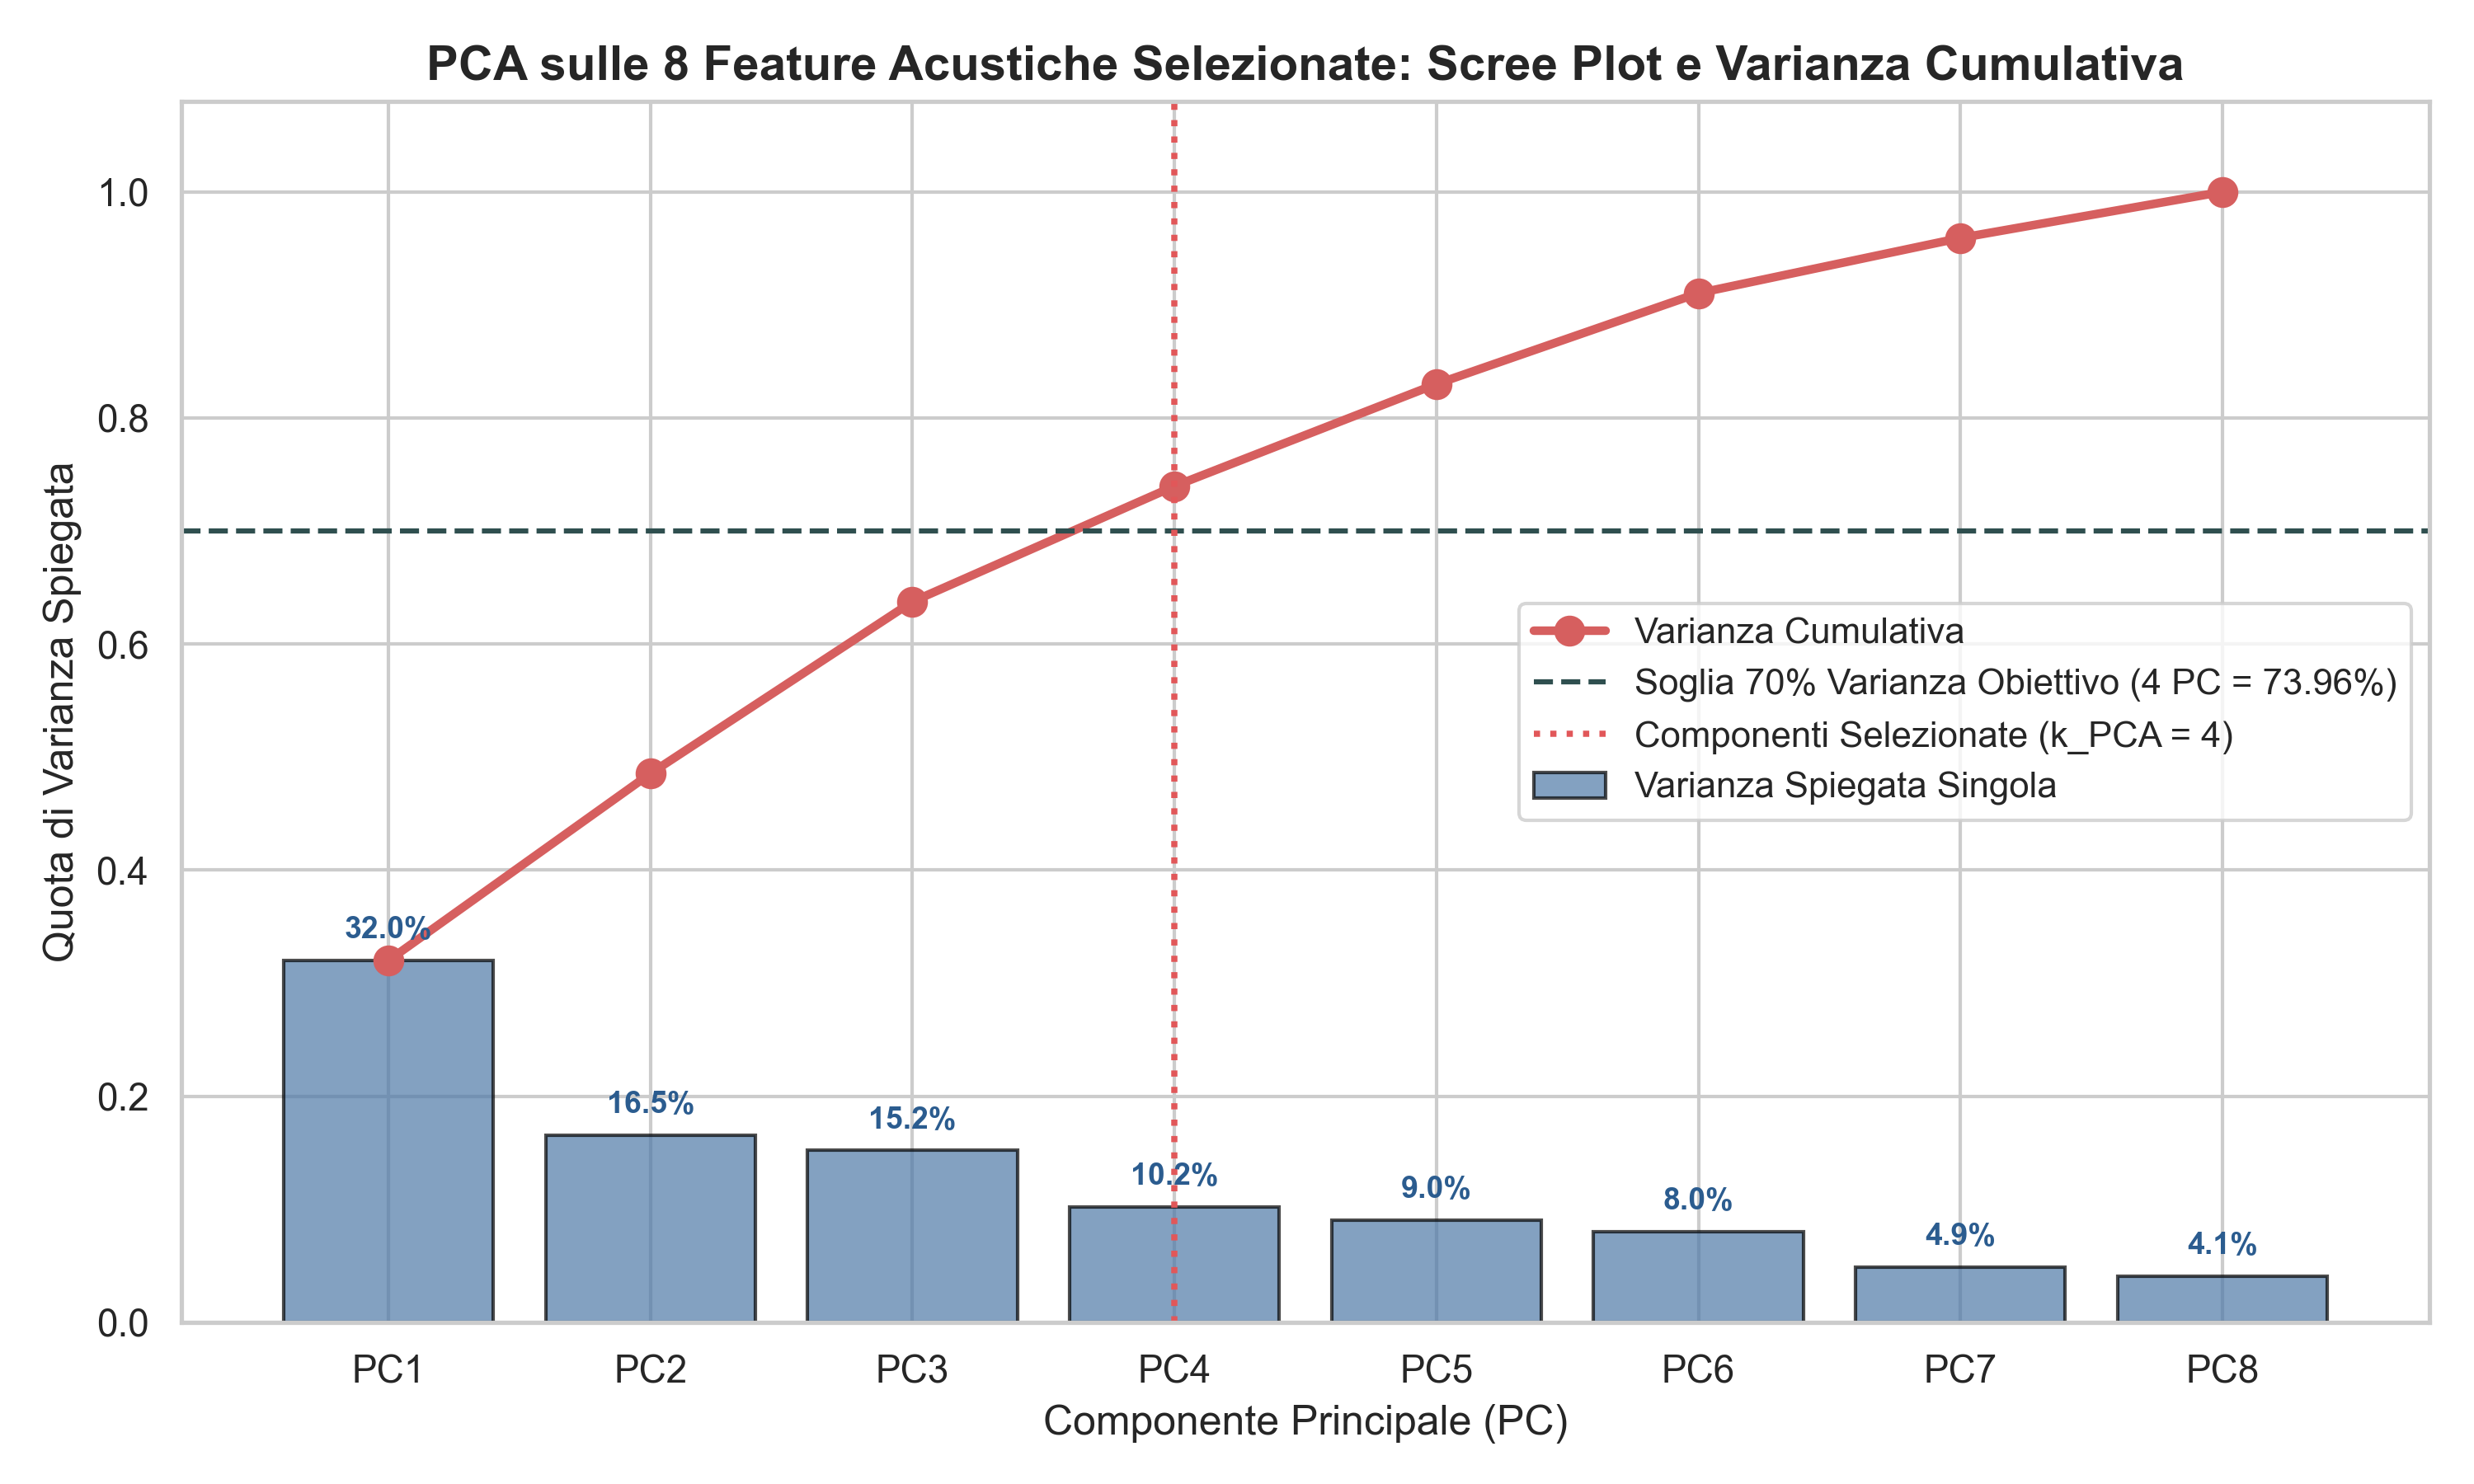
\includegraphics[width=0.78\textwidth]{capitolo4/img/fig14_pca_varianza_cumulativa.png}
    \caption{PCA sulle 8 feature acustiche: Scree Plot della varianza spiegata individuale e cumulativa con soglia obiettivo del 70\%.}
    \label{fig:pca_scree}
\end{figure}

Adottando il criterio della varianza cumulativa minima del 70\%, è stato scelto un numero di componenti pari a \textbf{$\text{n\_components} = 4$}, che preserva il \textbf{73,96\% della varianza totale} e dimezza la dimensionalità dello spazio (da 8 a 4 variabili latenti ortogonali). Il 26,04\% residuo non viene assunto automaticamente come rumore privo di informazione. K-Means, GMM, DBSCAN e HDBSCAN sono confrontati sulla matrice PCA a quattro dimensioni; t-SNE resta una tecnica di visualizzazione.

Ciascuna Componente Principale $\text{PC}_k$ ($k \in \{1, 2, 3, 4\}$) costituisce una nuova "super-variabile" latente ortogonale, ottenuta come combinazione lineare delle 8 feature standardizzate $z_{i,j}$ pesate attraverso i rispettivi coefficienti (\textit{PCA Loadings} $w_{j,k}$):
\begin{equation}
\boxed{\text{PC}_{i,k} = \sum_{j=1}^{8} w_{j,k} \, z_{i,j} = w_{1,k}\, z_{i,\text{dance}} + w_{2,k}\, z_{i,\text{energy}} + \dots + w_{8,k}\, z_{i,\text{duration}}}
\label{eq:pca_linear_comb}
\end{equation}
Per interpretare il significato fisico e musicale dei 4 assi latenti estratti, la Tabella \ref{tab:pca_loadings} riporta la matrice completa dei pesi $w_{j,k}$ che legano le 8 feature originarie alle prime 4 Componenti Principali.

\begin{table}[H]
\centering
\caption{Matrice dei Loadings (pesi lineari) delle prime 4 Componenti Principali rispetto alle 8 feature acustiche standardizzate.}
\label{tab:pca_loadings}
\vspace{0.2cm}
\begin{tabular}{lcccc}
\toprule
\textbf{Feature Acustica} & $\mathbf{PC_1}$ \textbf{(32,00\%)} & $\mathbf{PC_2}$ \textbf{(16,54\%)} & $\mathbf{PC_3}$ \textbf{(15,21\%)} & $\mathbf{PC_4}$ \textbf{(10,22\%)} \\
\midrule
\texttt{danceability}     & $-0,2179$ & $\mathbf{+0,6721}$ & $+0,2303$ & $+0,1679$ \\
\texttt{energy}           & $\mathbf{+0,3767}$ & $-0,2699$ & $\mathbf{+0,5122}$ & $-0,1522$ \\
\texttt{speechiness}      & $\mathbf{-0,3724}$ & $-0,0696$ & $+0,2895$ & $-0,0380$ \\
\texttt{acousticness}     & $\mathbf{-0,3482}$ & $+0,0925$ & $\mathbf{-0,5224}$ & $+0,2265$ \\
\texttt{instrumentalness} & $\mathbf{+0,4838}$ & $+0,2391$ & $-0,0819$ & $+0,3038$ \\
\texttt{valence}          & $-0,2888$ & $+0,2422$ & $\mathbf{+0,5533}$ & $+0,1739$ \\
\texttt{tempo}            & $-0,1770$ & $\mathbf{-0,5300}$ & $+0,1223$ & $\mathbf{+0,7626}$ \\
\texttt{duration\_ms}     & $\mathbf{+0,4494}$ & $+0,2555$ & $+0,0092$ & $\mathbf{+0,4380}$ \\
\bottomrule
\end{tabular}
\end{table}

Dall'ispezione dei coefficienti in Tabella \ref{tab:pca_loadings} emerge una chiara lettura semantica delle 4 dimensioni latenti:
\begin{itemize}
    \item $\mathbf{PC_1}$ \textbf{(32,00\% — Asse Strumentale/Elettronico Esteso vs. Vocale/Acustico Breve):} Presenta pesi positivi marcati su \texttt{instrumentalness} ($+0,4838$), \texttt{duration\_ms} ($+0,4494$) ed \texttt{energy} ($+0,3767$), contrapposti a pesi negativi su \texttt{speechiness} ($-0,3724$) e \texttt{acousticness} ($-0,3482$). Separa nettamente le lunghe tracce elettroniche da club prive di voce dalle canzoni brevi cantate o rappate.
    \item $\mathbf{PC_2}$ \textbf{(16,54\% — Asse Groove Ballabile Cadenzato vs. Velocità Ritmica):} È dominata positivamente dalla \texttt{danceability} ($+0,6721$) e negativamente dal \texttt{tempo} ($-0,5300$) e dall'\texttt{energy} ($-0,2699$). Distingue i brani dal groove cadenzato e ballabile (115--130 BPM) dalle tracce ad altissima velocità di battito e natura frenetica.
    \item $\mathbf{PC_3}$ \textbf{(15,21\% — Asse Euforia Elettrica vs. Intimità Acustica):} Combina contributi positivi elevati di \texttt{valence} ($+0,5533$) ed \texttt{energy} ($+0,5122$) con un forte contributo negativo di \texttt{acousticness} ($-0,5224$), discriminando i brani solari ed energici dalle ballate acustiche ed introspettive.
    \item $\mathbf{PC_4}$ \textbf{(10,22\% — Asse Velocità di Esecuzione e Durata):} È governata prevalentemente dal \texttt{tempo} ($+0,7626$) e da \texttt{duration\_ms} ($+0,4380$), isolando le variazioni puramente metriche e di velocità in BPM.
\end{itemize}

\newpage
\paragraph{t-SNE (t-Distributed Stochastic Neighbor Embedding):}
Accanto alla riduzione lineare PCA (usata per il calcolo effettivo dei cluster), è stata impiegata la tecnica non lineare t-SNE esclusivamente a scopo di visualizzazione topologica bidimensionale su un campione casuale rappresentativo di $N = 6.000$ brani (\texttt{n\_components=2}, \texttt{perplexity=40}, \texttt{random\_state=42}). La Figura \ref{fig:tsne_overview} mostra la mappa t-SNE colorata retrospettivamente con i 15 generi ufficiali di Spotify.

\begin{figure}[H]
    \centering
    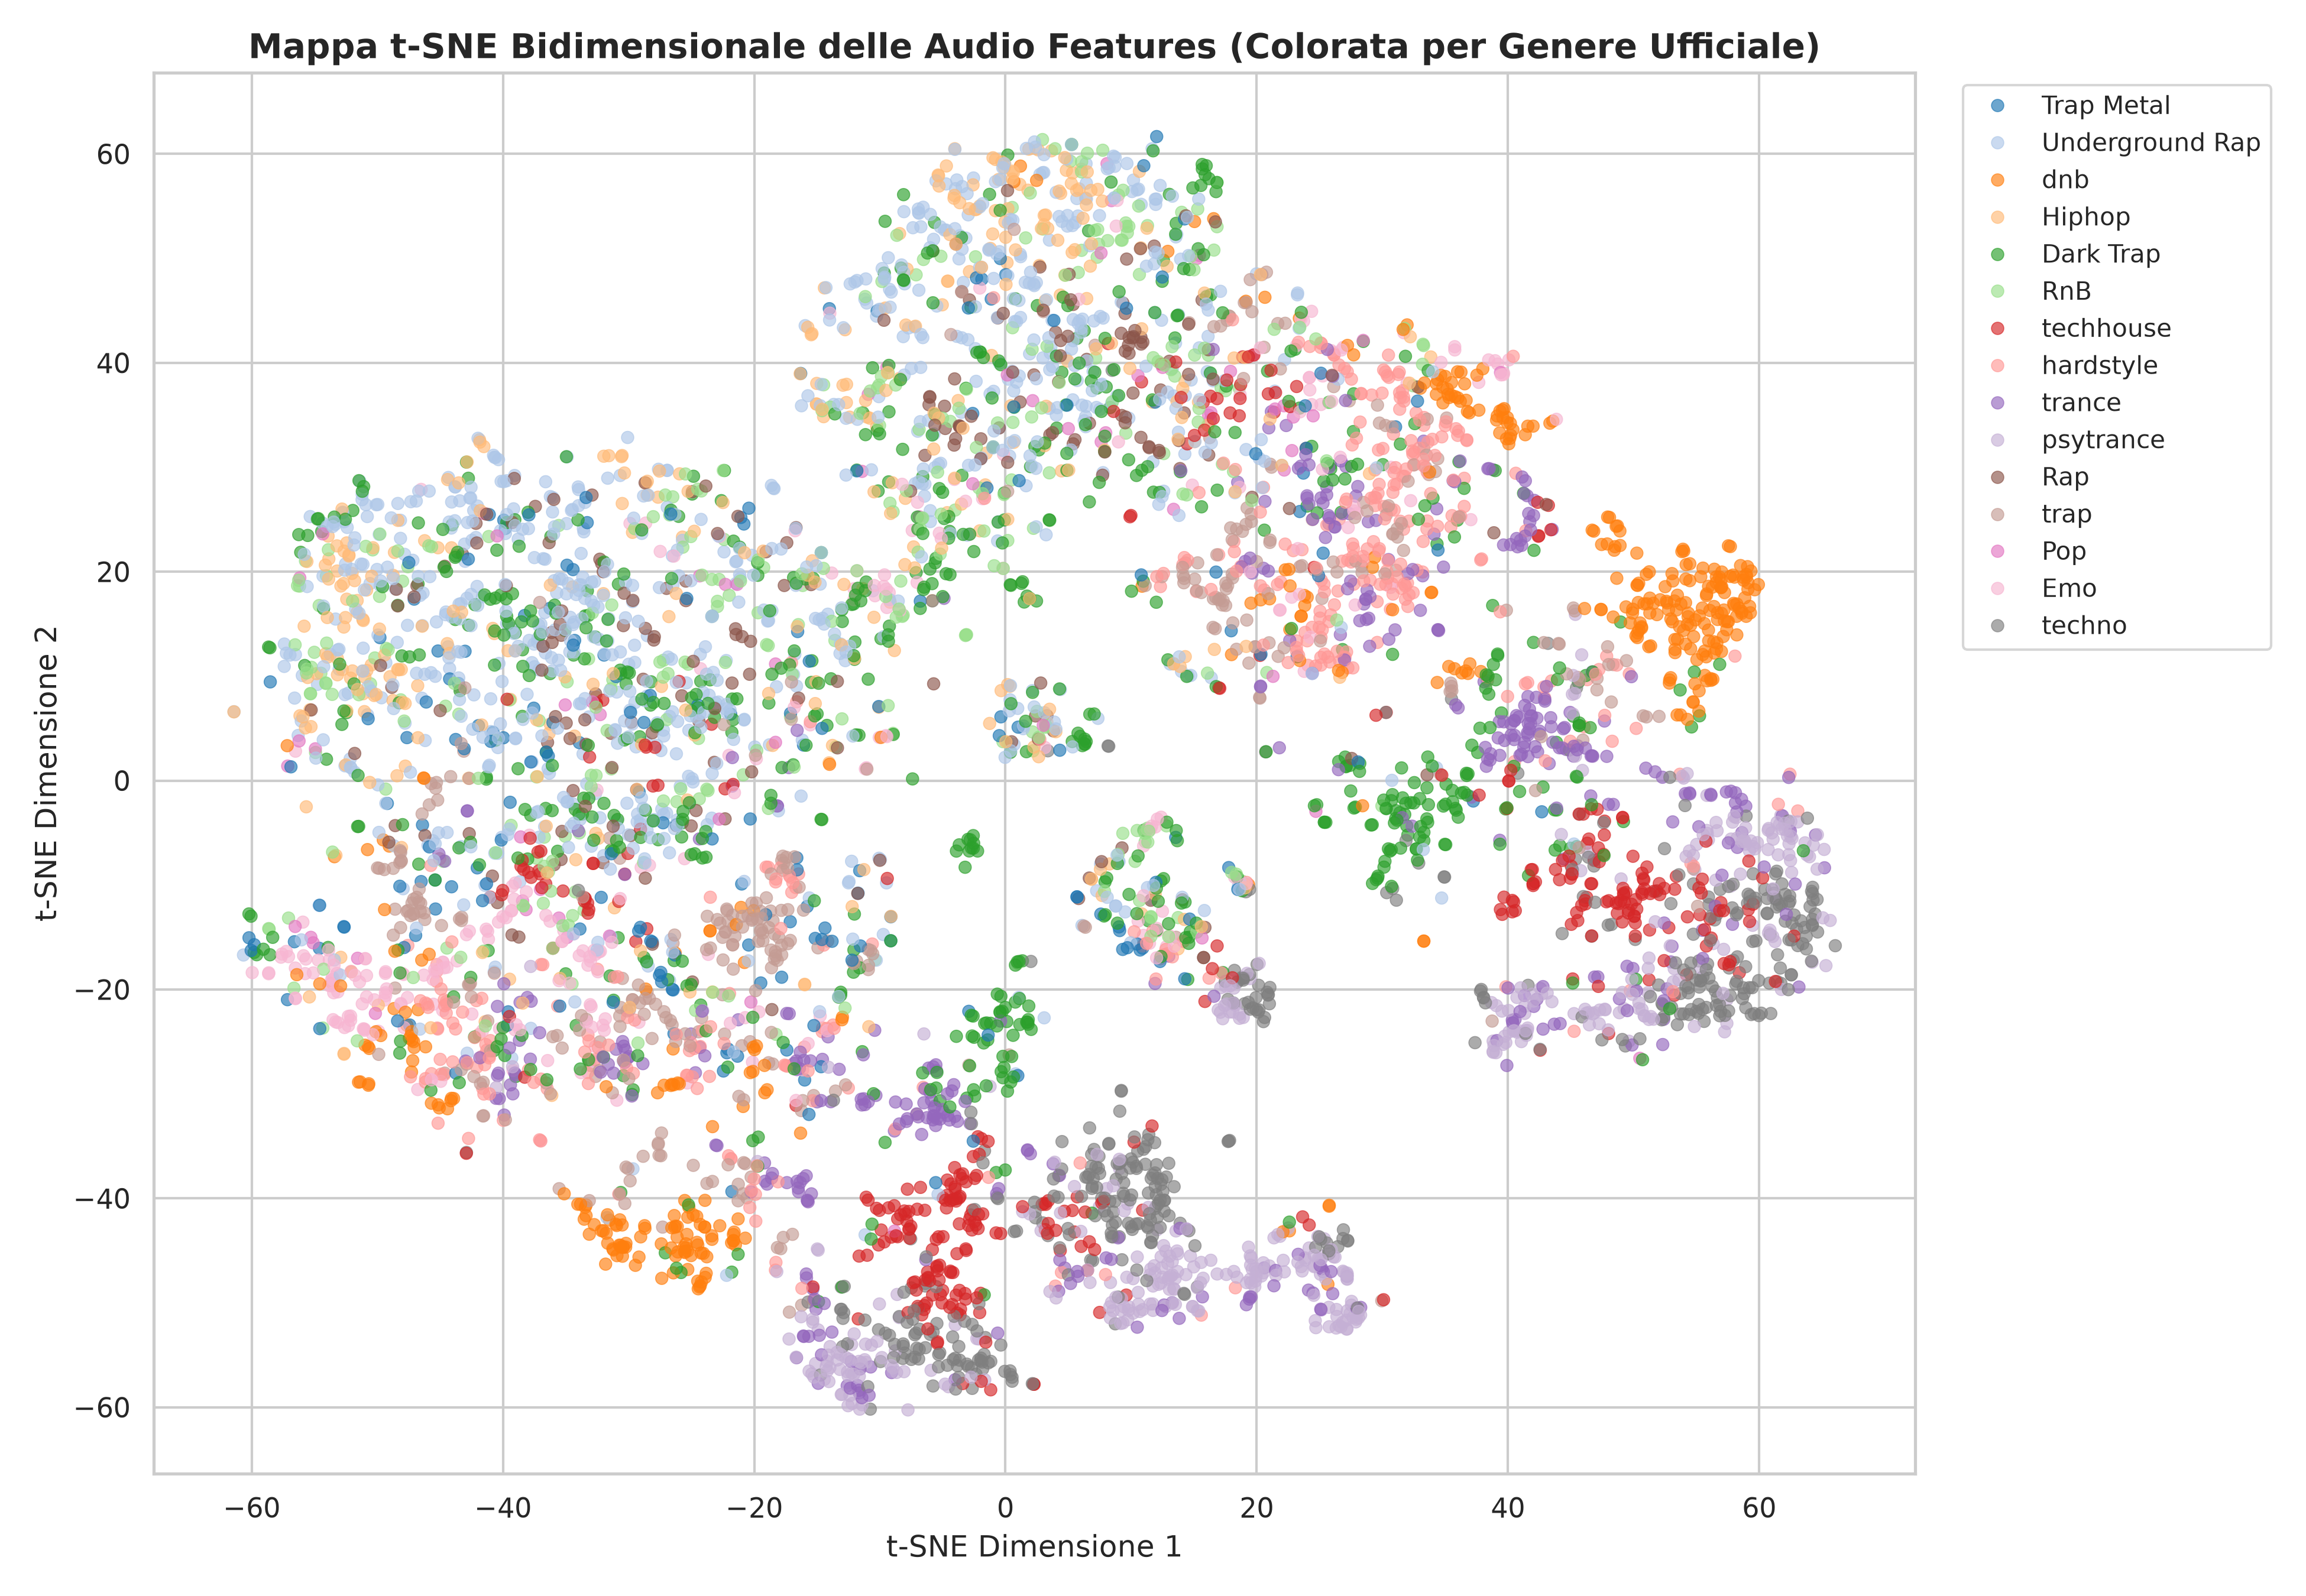
\includegraphics[width=0.86\textwidth]{capitolo4/img/fig15_tsne_2d_overview.png}
    \caption{Mappa 2D generata tramite t-SNE sulle feature acustiche, colorata retrospettivamente per genere Spotify originale.}
    \label{fig:tsne_overview}
\end{figure}

\newpage
\subsection{K-Means nello Spazio PCA}

Il metodo K-Means è un algoritmo di clustering per partizionamento che suddivide le $N$ osservazioni rappresentate nello spazio PCA a 4 dimensioni in $k$ cluster disgiunti $C_1, \dots, C_k$, minimizzando iterativamente la somma dei quadrati delle distanze euclidee intra-cluster (Within-Cluster Sum of Squares, WCSS):
\begin{equation}
\text{WCSS} = \sum_{j=1}^k \sum_{\mathbf{z}_i \in C_j} \|\mathbf{z}_i - \boldsymbol{\mu}_j\|^2
\label{eq:wcss}
\end{equation}
dove $\mathbf{z}_i \in \mathbb{R}^4$ è il vettore delle prime 4 componenti principali del brano $i$-esimo e $\boldsymbol{\mu}_j \in \mathbb{R}^4$ rappresenta il centroide del cluster $C_j$.

\subsubsection{Applicazione dell'algoritmo, Elbow Method e Coefficiente di Silhouette}

Per determinare in modo rigoroso il numero ottimale di cluster $k$ nello spazio PCA a 4 componenti, l'algoritmo K-Means (\texttt{n\_init=20}, \texttt{max\_iter=300}, \texttt{random\_state=42}) è stato valutato per $k \in \{2, 3, \dots, 10\}$ affiancando all'ispezione della curva d'inerzia WCSS (\textit{Elbow Method}) il calcolo del \textbf{Coefficiente di Silhouette medio}, come mostrato nel doppio grafico di Figura \ref{fig:kmeans_elbow}.

\begin{figure}[H]
    \centering
    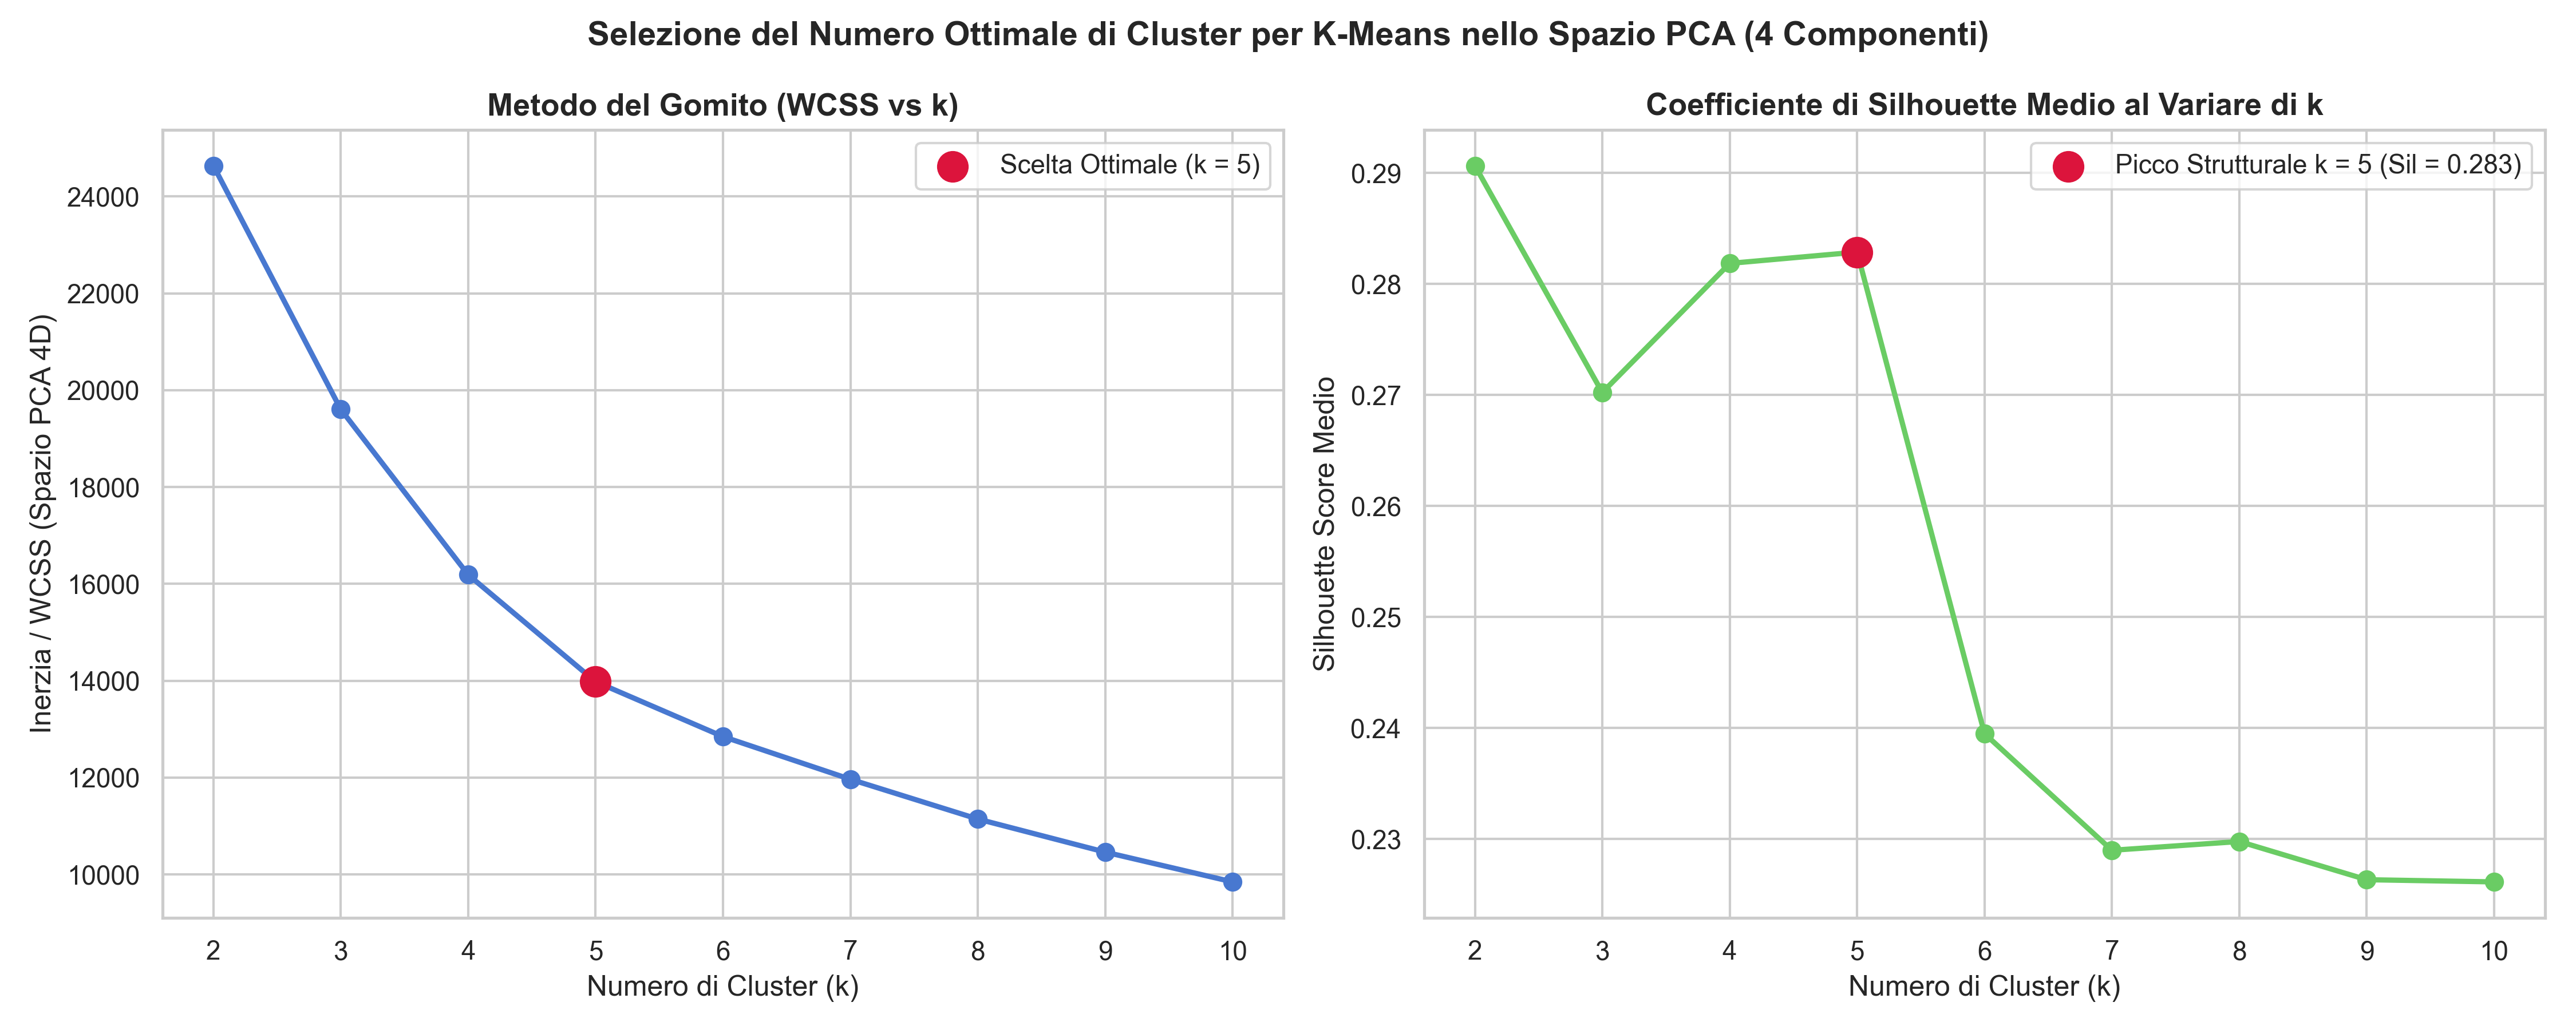
\includegraphics[width=0.95\textwidth]{capitolo4/img/fig16_kmeans_elbow_wcss.png}
    \caption{Selezione del parametro $k$ per K-Means nello spazio PCA (4 PC): curva WCSS (a sinistra) e Coefficiente di Silhouette medio (a destra).}
    \label{fig:kmeans_elbow}
\end{figure}

L'analisi congiunta dei due indicatori in Figura \ref{fig:kmeans_elbow} fornisce una giustificazione matematica univoca per la scelta di \textbf{$k = 5$}:
\begin{enumerate}
    \item Sulla curva WCSS (pannello sinistro), la pendenza subisce una netta decelerazione dopo $k = 5$ ($\text{WCSS} = 13.981,8$), punto oltre il quale l'aggiunta di ulteriori centroidi produce riduzioni marginali dell'inerzia intra-cluster.
    \item Sulla curva della Silhouette media (pannello destro), dopo i valori registrati a $k=3$ ($0,2702$) e $k=4$ ($0,2819$), la compattezza raggiunge un \textbf{massimo locale strutturale esattamente in corrispondenza di $k = 5$ con $\text{Silhouette} = 0,2829$}, prima di subire un brusco calo a $k = 6$ ($\text{Silhouette} = 0,2395$) dovuto alla frammentazione artificiale dei gruppi principali.
\end{enumerate}

\subsubsection{Analisi dei risultati ottenuti e proiezioni spaziali}

Il modello K-Means addestrato con $k = 5$ sulle 4 componenti principali ha generato una partizione bilanciata e ben strutturata sia sul campione di analisi ($N = 6.000$) sia sull'intero catalogo deduplicato ($N = 35.877$), come riepilogato nella Tabella \ref{tab:kmeans_counts}.

\begin{table}[H]
\centering
\caption{Distribuzione numerica e percentuale dei brani nei 5 cluster K-Means (campione di analisi e intero catalogo deduplicato).}
\label{tab:kmeans_counts}
\vspace{0.2cm}
\resizebox{\textwidth}{!}{%
\begin{tabular}{llccc}
\toprule
\textbf{Cluster} & \textbf{Archetipo Musicale (Mood Playlist)} & \textbf{Campione ($N=6.000$)} & \textbf{Catalogo ($N=35.877$)} & \textbf{Quota (\%)} \\
\midrule
\textbf{Cluster 0} & High-Intensity Bass \& Workout        & 1.710 & 10.583 & 29,50\% \\
\textbf{Cluster 1} & Extended Club \& Instrumental         & 1.517 & 8.964  & 24,99\% \\
\textbf{Cluster 2} & Acoustic, Chill \& Atmospheric        & 549   & 3.189  & 8,89\%  \\
\textbf{Cluster 3} & Groove, Melodic Urban \& Dance-Pop    & 1.250 & 7.354  & 20,50\% \\
\textbf{Cluster 4} & Fast-Flow Rap \& High-Tempo Urban     & 974   & 5.787  & 16,13\% \\
\bottomrule
\end{tabular}}
\end{table}

La Figura \ref{fig:kmeans_tsne} illustra la disposizione geometrica dei 5 cluster affiancando la proiezione lineare nel piano delle prime due componenti principali ($\text{PC}_1$ vs $\text{PC}_2$, con indicazione esplicita dei 5 centroidi $\mathbf{X}$) e la proiezione non lineare sulla mappa t-SNE.

\begin{figure}[H]
    \centering
    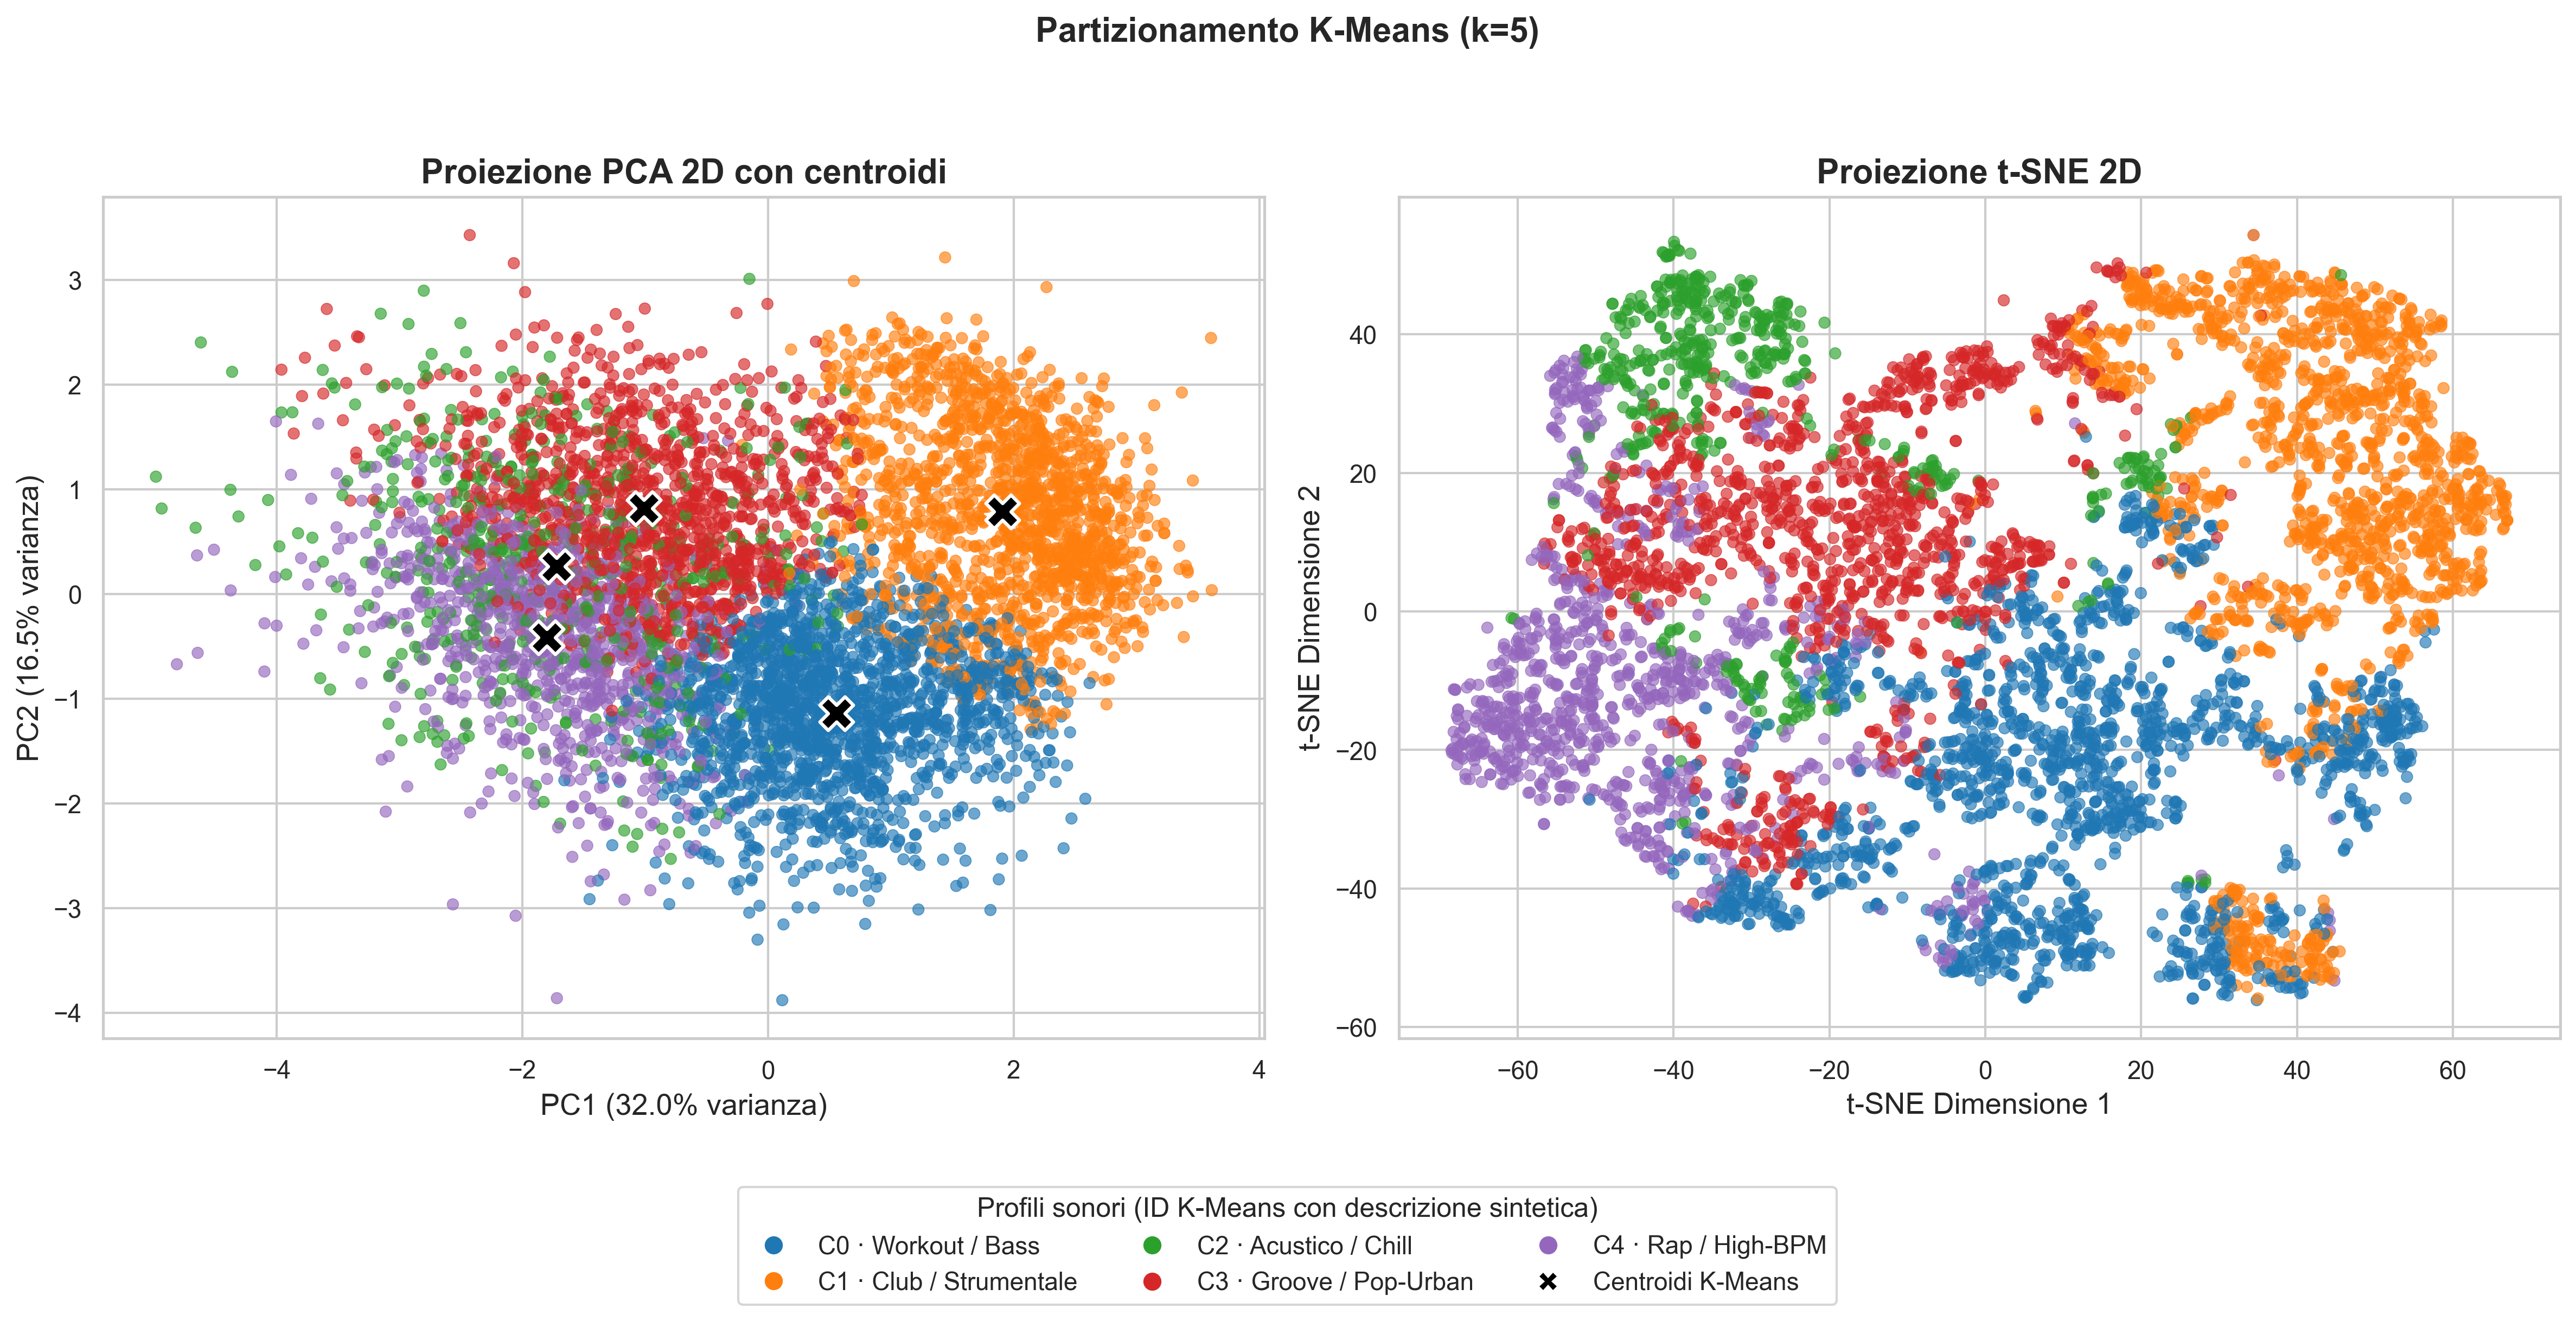
\includegraphics[width=0.98\textwidth]{capitolo4/img/fig17_kmeans_tsne_clusters.png}
    \caption{Partizionamento K-Means ($k=5$) visualizzato nel piano lineare PCA ($\text{PC}_1$ vs $\text{PC}_2$ con centroidi) e sulla mappa non lineare t-SNE 2D.}
    \label{fig:kmeans_tsne}
\end{figure}

Dalla Figura \ref{fig:kmeans_tsne} si osserva come nel piano PCA i 5 centroidi presidino regioni ben distinte dello spazio delle componenti principali, e come tale partizione si traduca, sulla varietà non lineare t-SNE, in macro-regioni timbriche coerenti e prive di sovrapposizioni caotiche.

\newpage
\subsubsection{Profiling acustico dei Cluster e Mood Playlists}

Per interpretare il significato musicale e funzionale dei 5 cluster, la Figura \ref{fig:kmeans_profile_heatmap} riporta una heatmap delle medie osservate. Le annotazioni contengono i valori medi originali (la durata è espressa in migliaia di millisecondi), mentre il colore è normalizzato Min-Max separatamente per ciascuna feature: il colore consente quindi di confrontare i cluster sulla stessa variabile, non grandezze assolute tra variabili diverse. La matrice include anche \texttt{loudness} e \texttt{liveness} come descrittori retrospettivi; queste due variabili non sono state usate per addestrare K-Means né per costruire lo spazio PCA.

\begin{figure}[H]
    \centering
    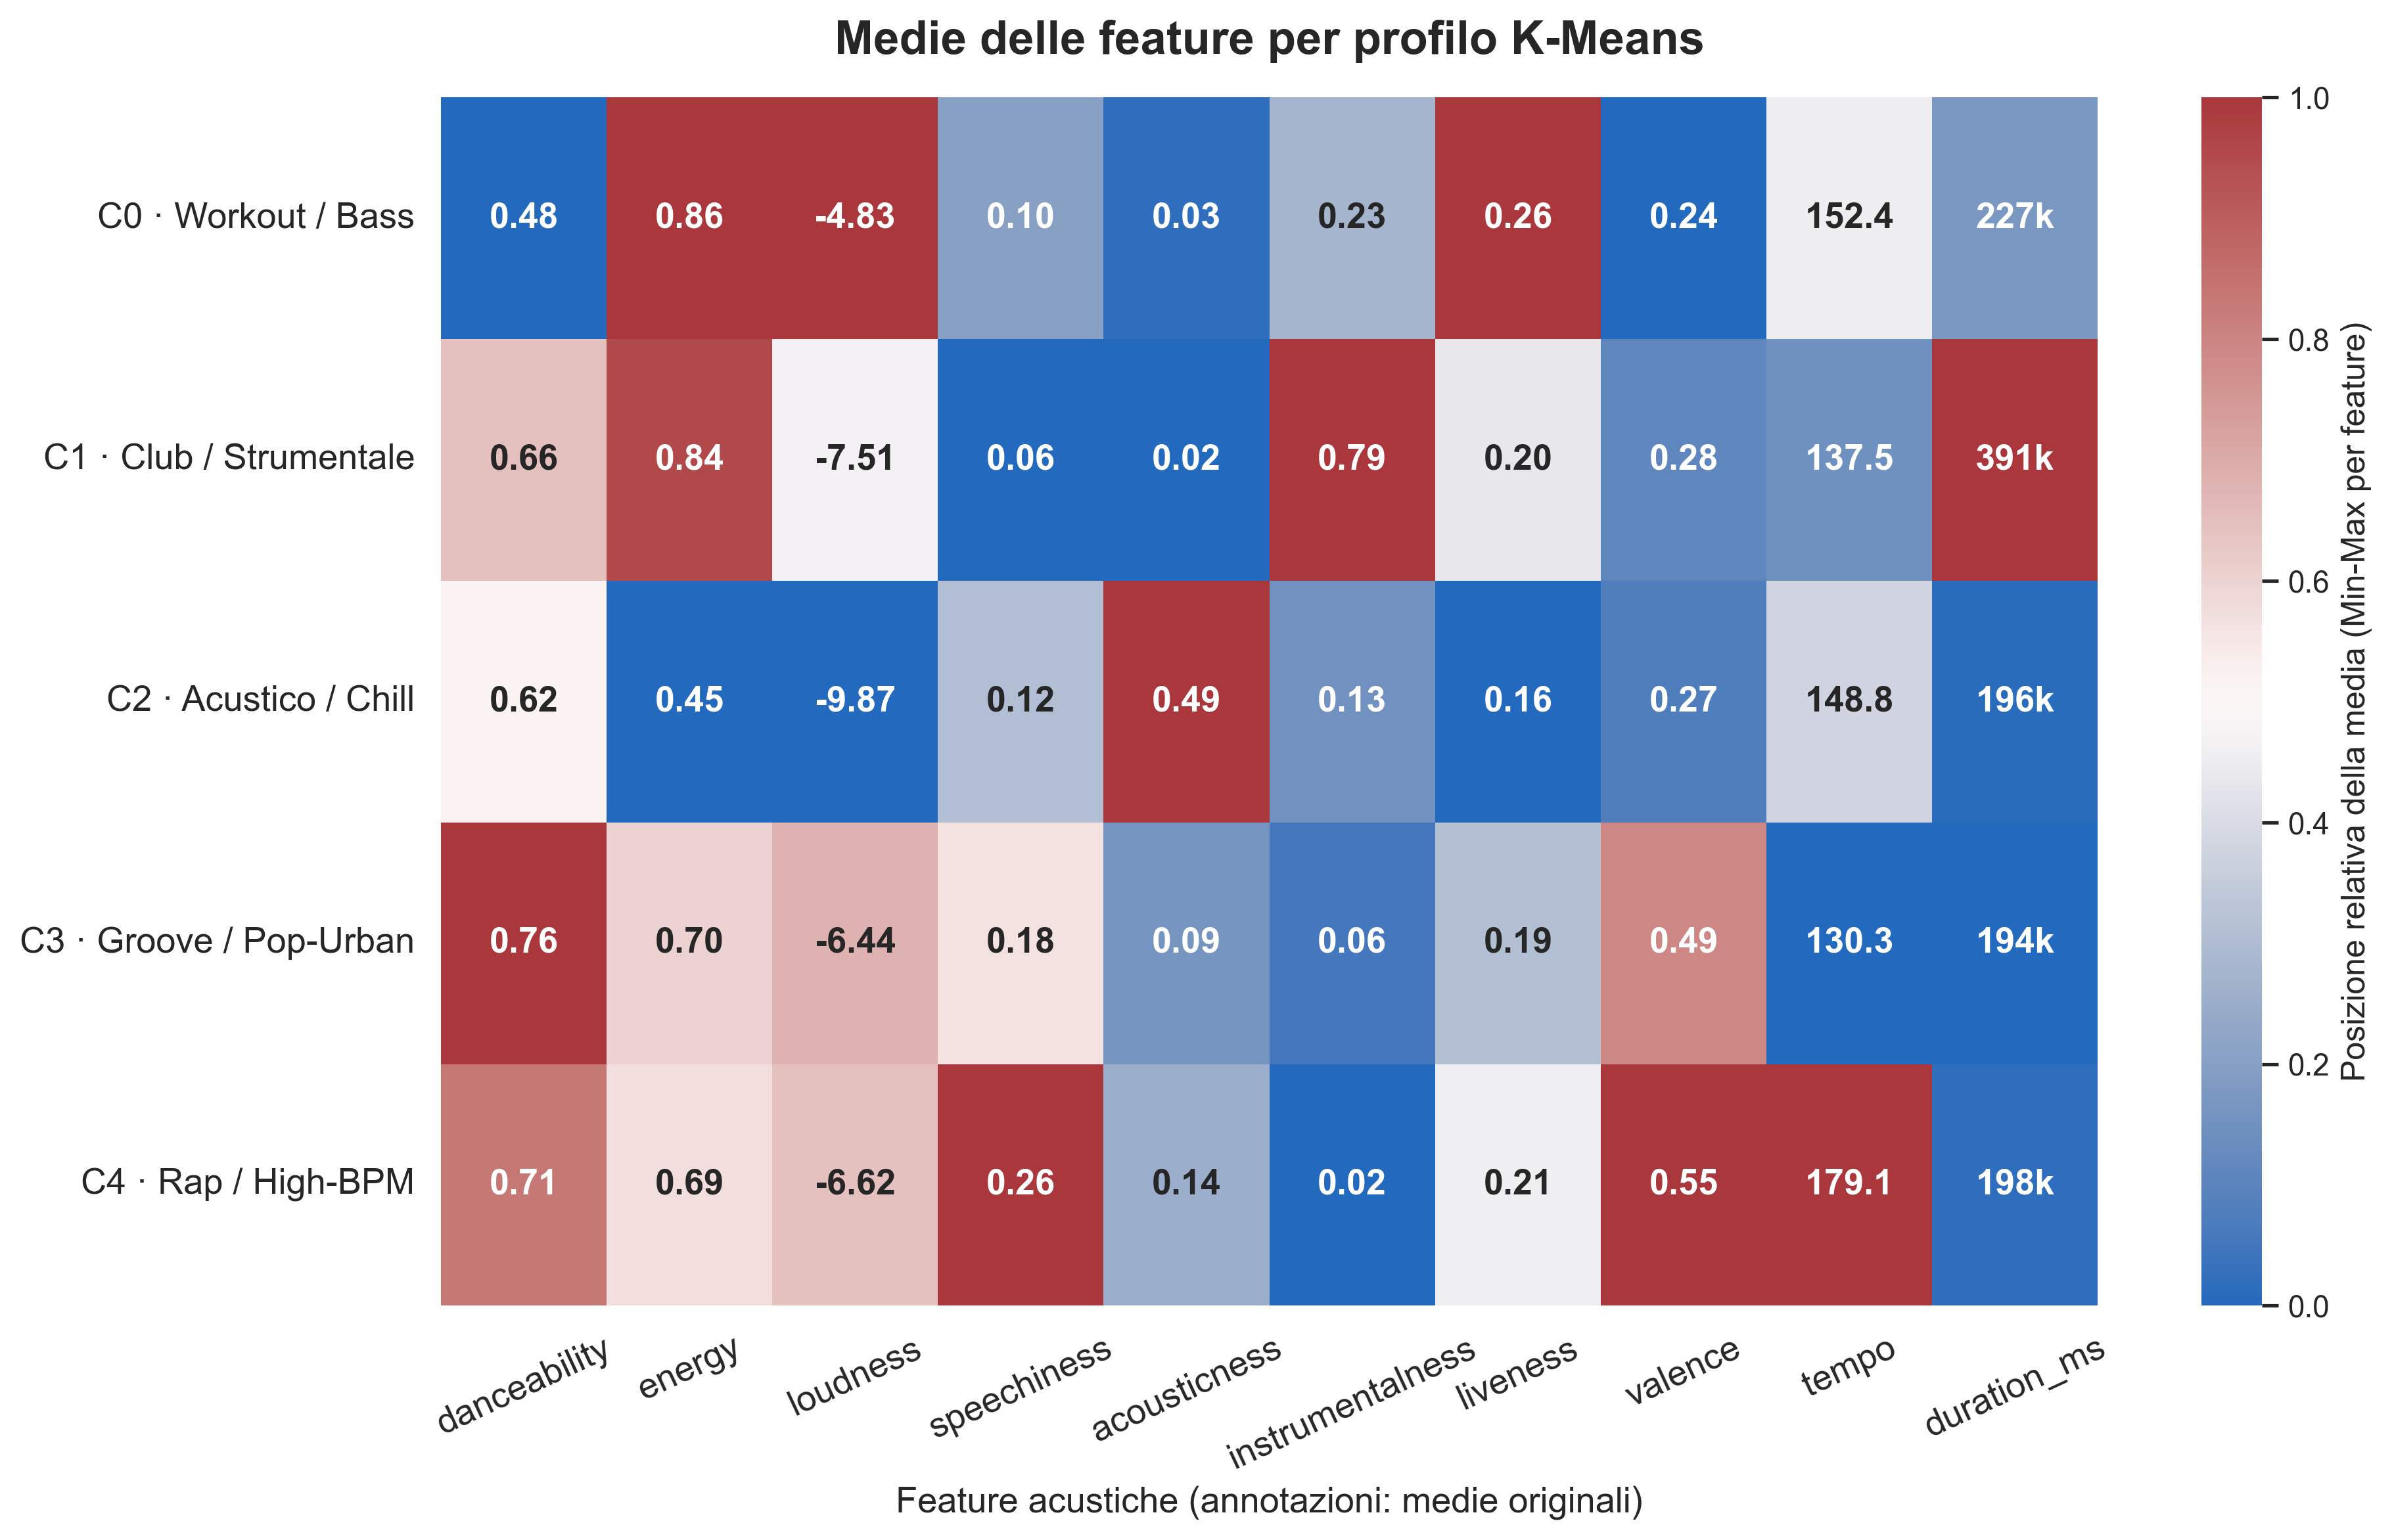
\includegraphics[width=\textwidth]{capitolo4/img/fig18_kmeans_feature_profiling.png}
    \caption{Medie delle feature per i cluster K-Means. Le annotazioni riportano le medie originali; il colore è riscalato per colonna.}
    \label{fig:kmeans_profile_heatmap}
\end{figure}

La matrice mette in evidenza differenze utili a descrivere i profili: C1 presenta una forte strumentalità e durate maggiori; C2 ha maggiore acusticità e minore energia; C3 è il profilo più ballabile, mentre C4 mostra tempo e contenuto parlato più elevati. C0 combina energia e volume mediamente alti. Le sigle C0--C4 sono identificativi; i nomi brevi riportati in legenda riassumono i tratti dominanti, senza essere etichette di genere.

La Figura \ref{fig:kmeans_profile_radar} visualizza in forma polare gli stessi profili limitandosi alle 8 feature effettivamente usate nel clustering. Anche in questo grafico ciascun asse è normalizzato tra i cluster: la forma rende immediato il confronto relativo tra profili, ma non va letta come confronto delle unità originali o come intensità assoluta della feature.

\begin{figure}[H]
    \centering
    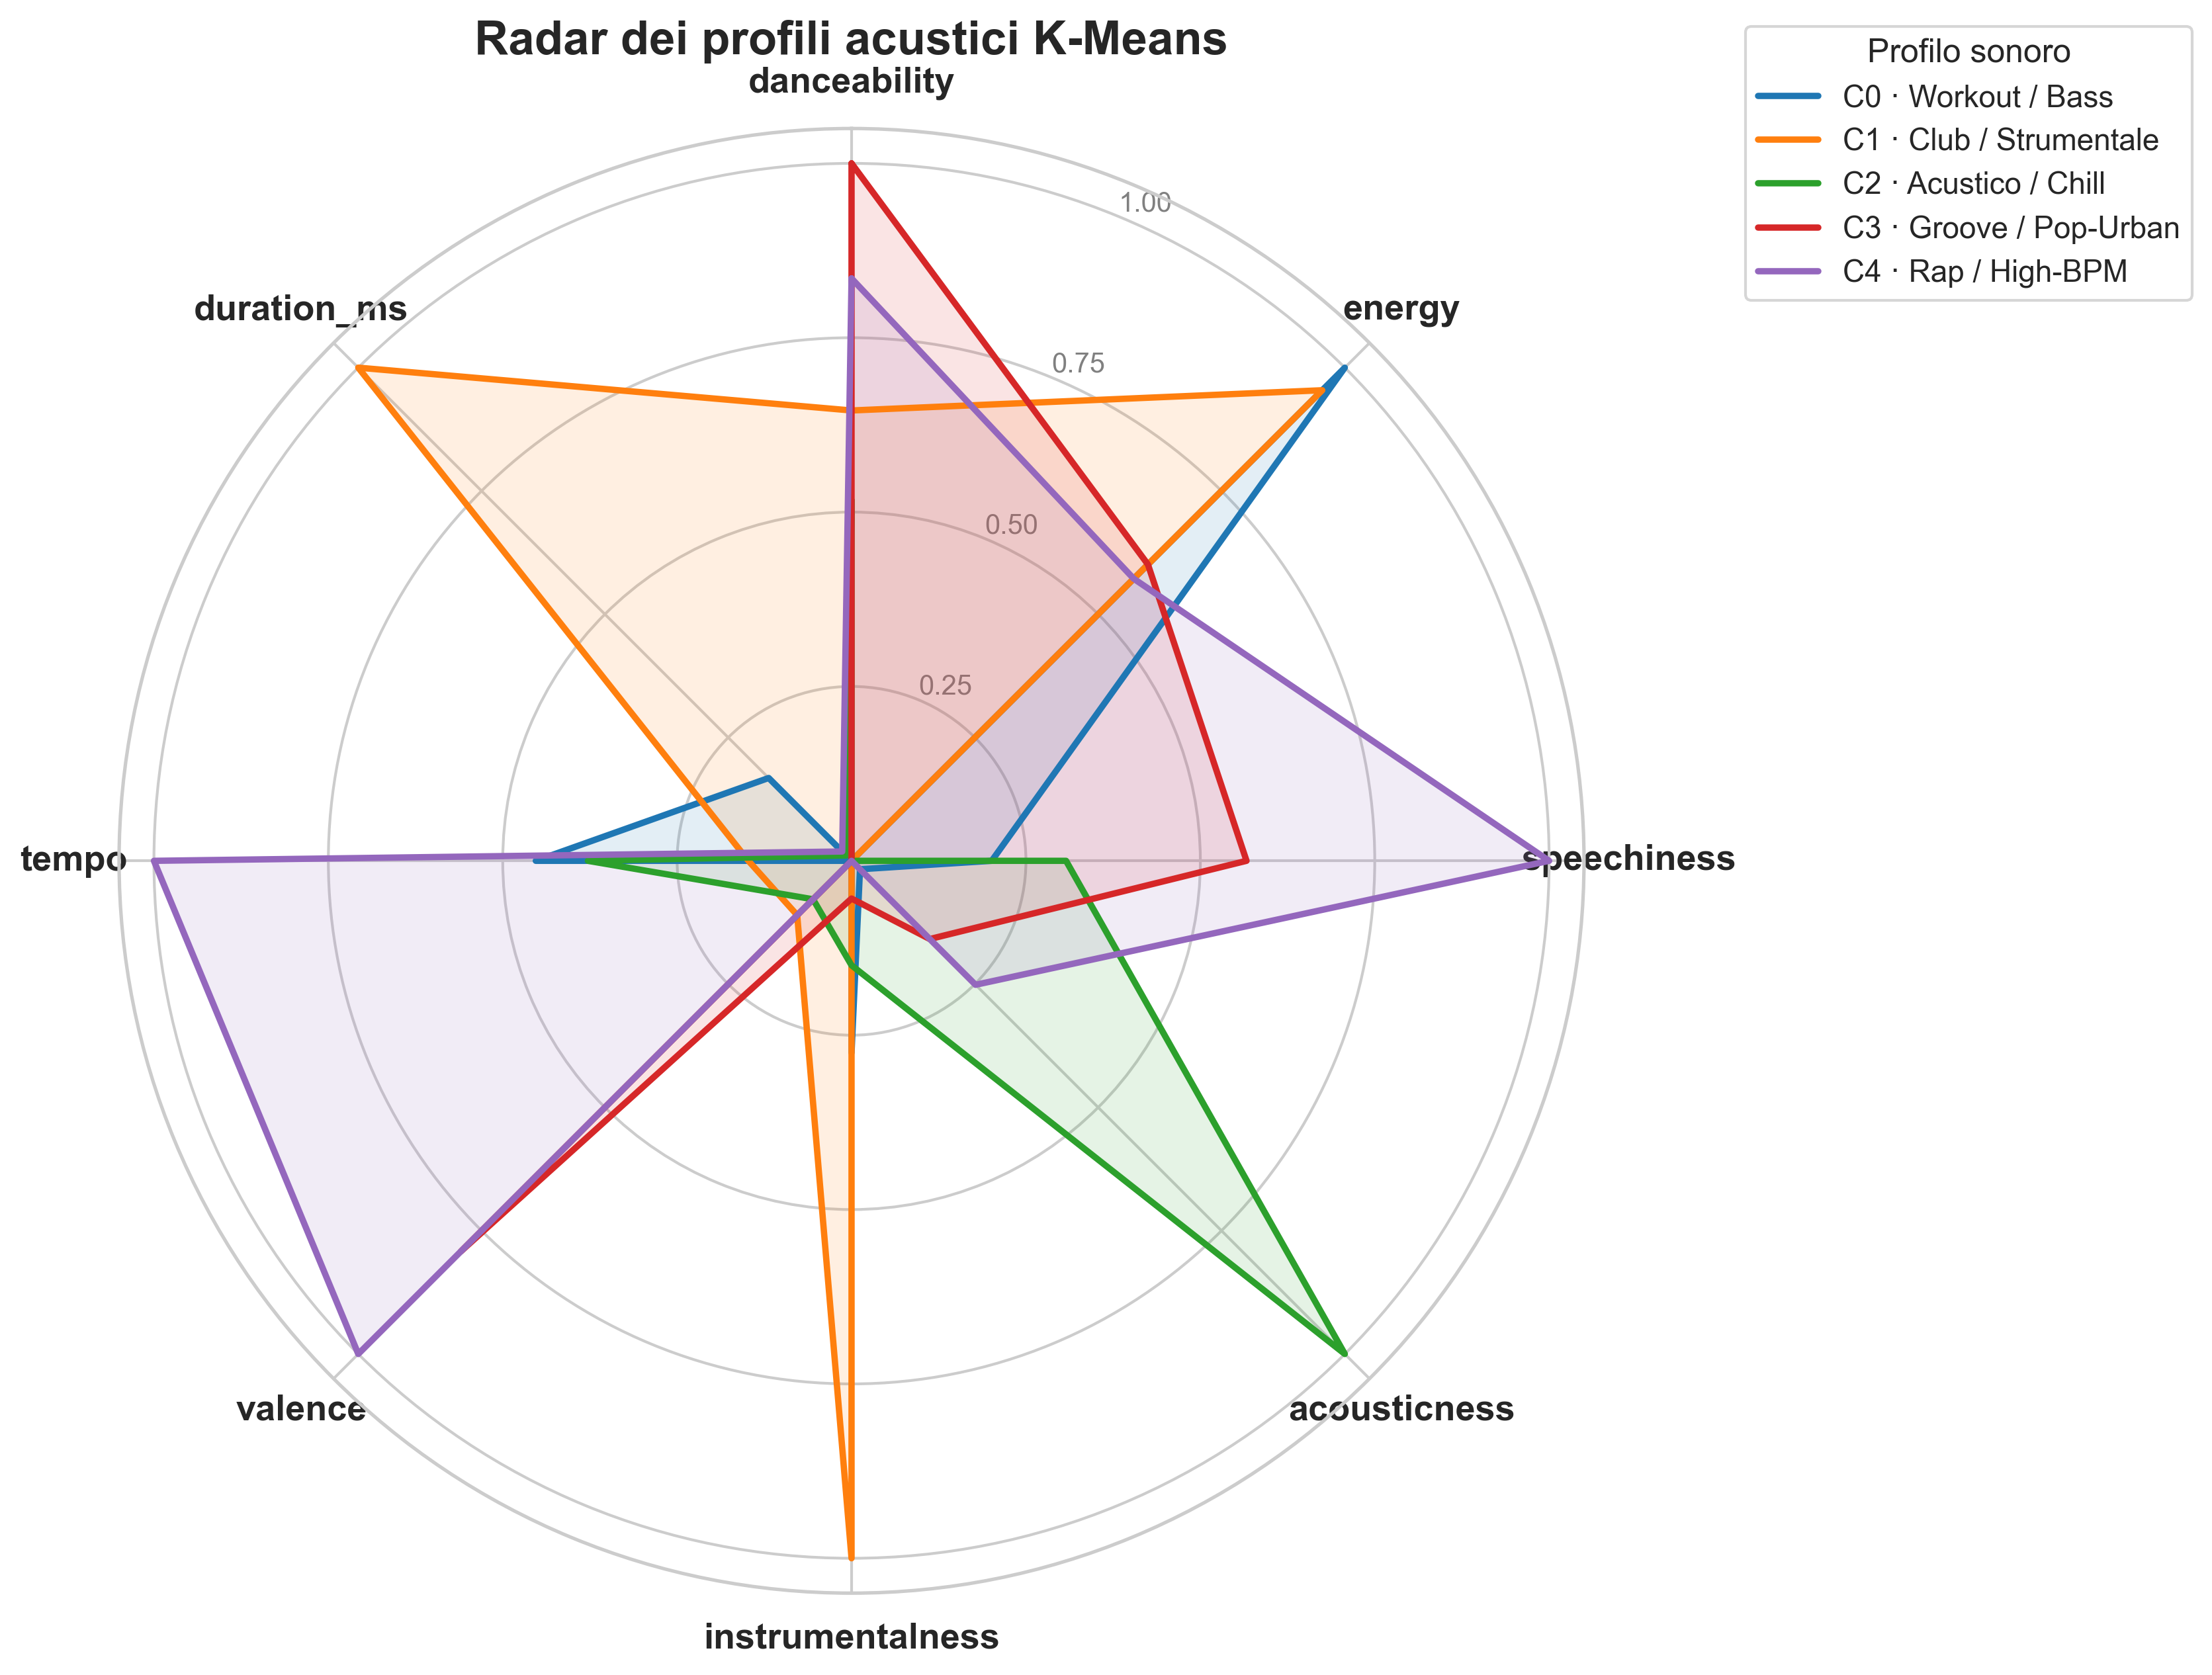
\includegraphics[width=0.98\textwidth]{capitolo4/img/fig19_kmeans_feature_radar.png}
    \caption{Radar chart delle medie normalizzate delle 8 feature usate nel clustering K-Means.}
    \label{fig:kmeans_profile_radar}
\end{figure}

Dall'esame congiunto delle Figure \ref{fig:kmeans_profile_heatmap} e \ref{fig:kmeans_profile_radar}, oltre che dall'incrocio retrospettivo con i generi originali, ciascun cluster rivela un'identità acustica e funzionale netta:
\begin{itemize}
    \item \textbf{Cluster 0 — High-Intensity Bass \& Workout ($1.710$ brani campione / $10.583$ catalogo):} È il cluster a massima potenza d'urto: registra i valori medi più elevati in assoluto di \texttt{energy} ($0,86$) e \texttt{loudness} ($-4,83\text{ dB}$), uniti a un \texttt{tempo} sostenuto ($152,40\text{ BPM}$), ma con la più bassa \texttt{danceability} ($0,48$) e una \texttt{valence} scura/aggressiva ($0,24$). Raccoglie in larga misura tracce \textit{Hardstyle}, \textit{Drum and Bass} e \textit{Trap/Trap Metal} ad alto impatto adrenalinico, perfette per playlist di allenamento intenso (\textit{Workout / Gym}).
    \item \textbf{Cluster 1 — Extended Club \& Instrumental Electronic ($1.517$ brani campione / $8.964$ catalogo):} Si distingue in modo inequivocabile per l'altissima \texttt{instrumentalness} media ($0,79$, contro $0,02\text{--}0,23$ degli altri gruppi) e per la durata media estesa (\texttt{duration\_ms} $= 390.803\text{ ms}$, circa $6,5$ minuti), accompagnate da \texttt{energy} elevata ($0,84$), ottima \texttt{danceability} ($0,66$), \texttt{speechiness} minima ($0,06$) e battito regolare da club ($137,52\text{ BPM}$). Cattura i brani \textit{Techno}, \textit{Psytrance}, \textit{Trance} e \textit{Techhouse} pensati per il DJ mixing e per sessioni di \textit{Deep Focus / Clubbing}.
    \item \textbf{Cluster 2 — Acoustic, Chill \& Atmospheric ($549$ brani campione / $3.189$ catalogo):} Rappresenta il polo intimo e decompressivo del catalogo: presenta il valore massimo di \texttt{acousticness} ($0,49$, oltre tre volte superiore a qualsiasi altro cluster) e i livelli minimi di \texttt{energy} ($0,45$) e volume (\texttt{loudness} $= -9,87\text{ dB}$), con durata contenuta ($196.127\text{ ms}$). Raggruppa produzioni acustiche, R\&B morbido, Emo e tracce \textit{Dark Trap / Lo-Fi} rarefatte, ideali per playlist \textit{Chillout, Late Night \& Relax}.
    \item \textbf{Cluster 3 — Groove, Melodic Urban \& Dance-Pop ($1.250$ brani campione / $7.354$ catalogo):} È il cluster a più alta ballabilità dell'intero dataset (\texttt{danceability} $= 0,76$), caratterizzato da un \texttt{tempo} moderato e cadenzato ($130,31\text{ BPM}$), \texttt{valence} positiva ($0,49$), buona \texttt{energy} ($0,70$), presenza vocale ritmica (\texttt{speechiness} $= 0,18$) e quasi totale assenza strumentale ($0,06$). Aggrega in modo trasversale \textit{Pop}, \textit{R\&B}, \textit{Rap melodico} e \textit{Techhouse} radiofonica, costituendo l'archetipo perfetto per playlist \textit{Social Groove \& Aperitif}.
    \item \textbf{Cluster 4 — Fast-Flow Rap \& High-Tempo Urban ($974$ brani campione / $5.787$ catalogo):} Isola i brani caratterizzati dalla massima velocità ritmica (\texttt{tempo} medio $= 179,12\text{ BPM}$), dalla massima densità di parlato/rima (\texttt{speechiness} $= 0,26$) e dalla più alta positività/dinamismo (\texttt{valence} $= 0,55$), con \texttt{danceability} elevata ($0,71$) e durata compatta ($197.699\text{ ms}$). È composto prevalentemente da \textit{Underground Rap}, \textit{Hiphop} e \textit{Dark Trap} in doppia metrica, ideale per playlist \textit{Street Flow \& High-BPM Urban}.
\end{itemize}

\newpage
\subsubsection{Valutazione della Silhouette per K-Means}

Per valutare la coesione interna e la separazione di ciascuno dei 5 gruppi individuati nello spazio PCA a 4 dimensioni, è stato calcolato il coefficiente di Silhouette puntuale $s(i)$ per ogni brano del campione secondo la formula:
\begin{equation}
s(i) = \frac{b(i) - a(i)}{\max(a(i), b(i))}
\label{eq:silhouette}
\end{equation}
dove $a(i)$ è la distanza euclidea media tra il brano $i$ e gli altri brani del medesimo cluster nello spazio PCA 4D, mentre $b(i)$ è la distanza media minima rispetto ai brani del cluster contiguo più vicino. La Figura \ref{fig:kmeans_silhouette} mostra la distribuzione dei coefficienti di Silhouette per i 5 cluster.

\begin{figure}[H]
    \centering
    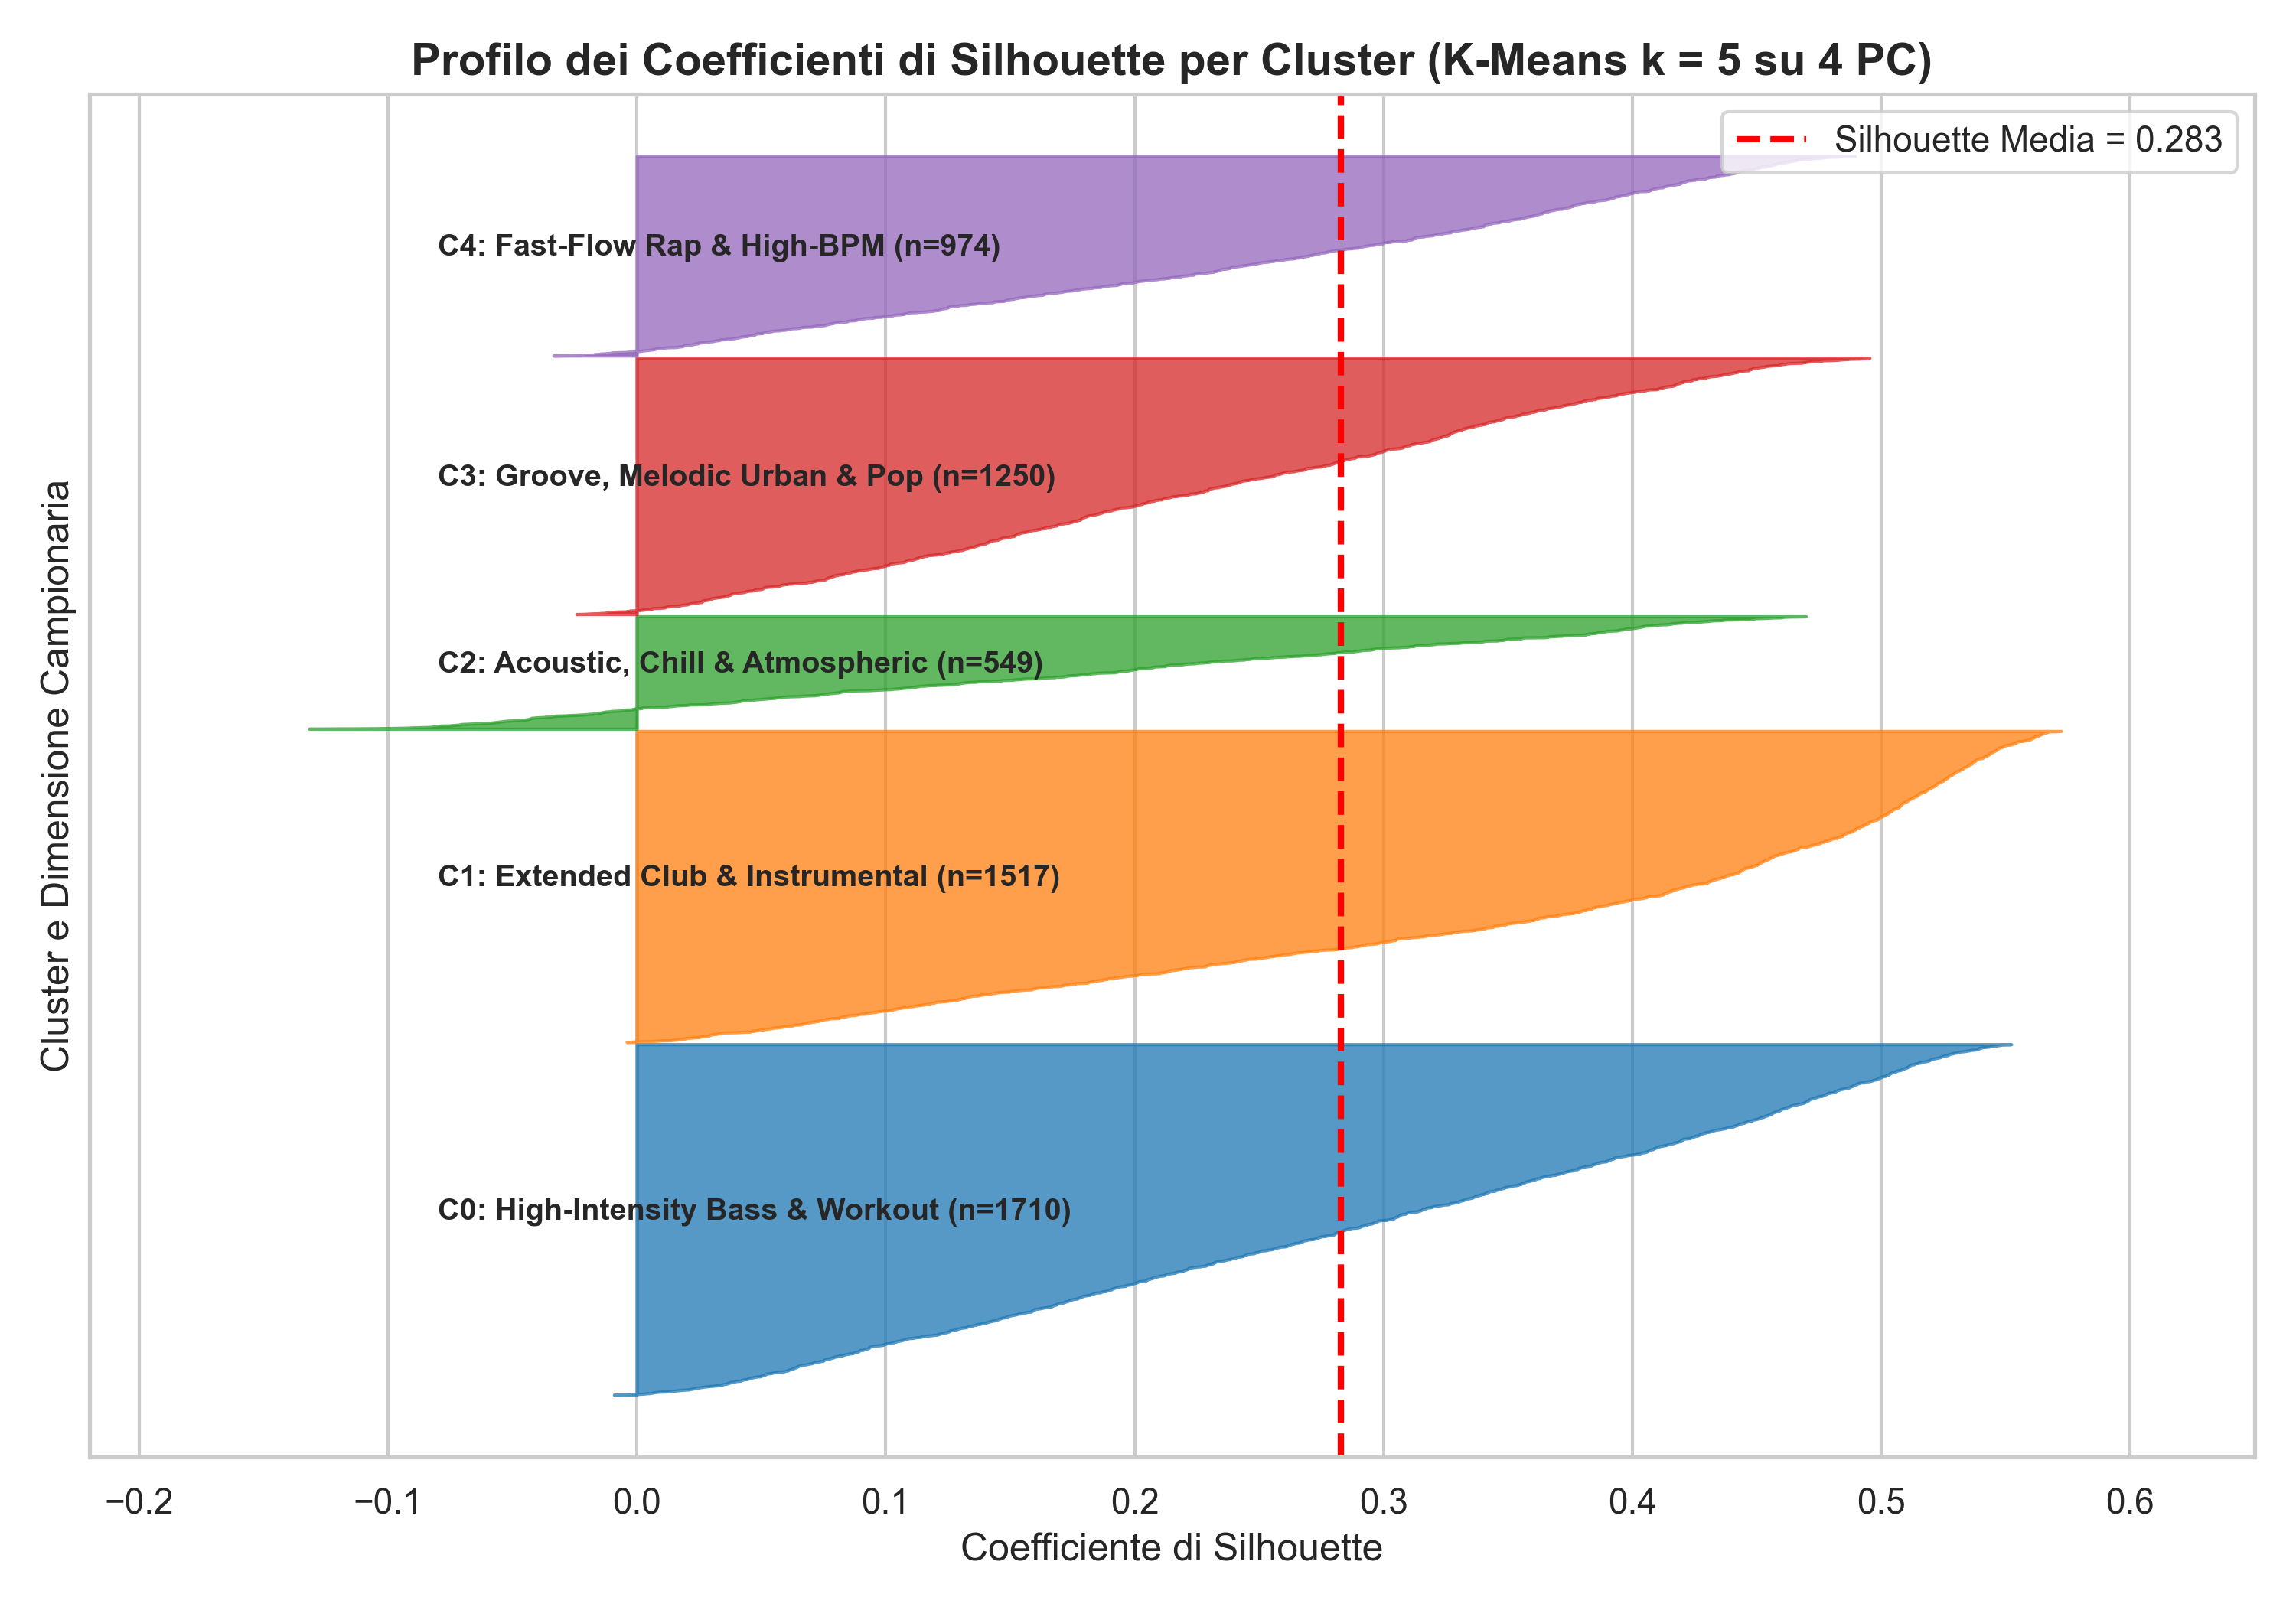
\includegraphics[width=0.78\textwidth]{capitolo4/img/fig19_kmeans_silhouette_plot.png}
    \caption{Profilo dei coefficienti di Silhouette per ciascun cluster K-Means ($k=5$) calcolato nello spazio PCA a 4 componenti.}
    \label{fig:kmeans_silhouette}
\end{figure}

Dalla Figura \ref{fig:kmeans_silhouette} emerge un valore medio globale di Silhouette pari a \textbf{$0,2829$} (notevolmente superiore al valore di $0,1204$ che si otterrebbe applicando K-Means direttamente sulle 13 variabili non ridotte). Tutti e 5 i cluster superano ampiamente la soglia media con picchi superiori a $0,50$ (in particolare il Cluster 1 strumentale e i Cluster 3 e 4 urban/groove) e una frazione molto ridotta di valori negativi (punti di confine). Un valore di Silhouette intorno a $0,28\text{--}0,30$ è pienamente coerente con la natura fisica dei dati musicali: a differenza di dataset sintetici con isole disgiunte, gli attributi acustici formano una varietà continua in cui le transizioni tra stili avvengono gradualmente, e K-Means opera efficacemente una tassonomia geometrica convessa di tale continuum.

\subsubsection{Evoluzione probabilistica di K-Means: Gaussian Mixture Model}
K-Means assegna ciascun brano in modo deterministico e rigido a un solo cluster, anche quando le sue coordinate metriche cadono esattamente nella terra di nessuno tra due o più profili. Nel dominio musicale, tuttavia, i generi e gli stati emotivi formano un continuum sfumato: una traccia \textit{RnB contemporanea} può combinare un groove ritmico ballabile con una timbrica vocale intima ed acustica, rendendo riduttiva l'assegnazione a un singolo contenitore disgiunto. Per superare questa limitazione geometrica e catturare la natura polivalente della musica, è stato introdotto un \textit{Gaussian Mixture Model} (GMM) a cinque componenti con matrice di covarianza piena (\texttt{covariance\_type='full'}), addestrato sul medesimo campione di $N=6.000$ brani nello spazio PCA a 4 dimensioni.

Il modello stima per ogni traccia un vettore di affiliazioni probabilistiche $\boldsymbol{\gamma}_i = (\gamma_{i,0}, \dots, \gamma_{i,4})$, dove $\sum_{k=0}^4 \gamma_{i,k} = 1$. Questi valori quantificano l'appartenenza a ciascuno dei 5 macro-archetipi nello spazio acustico latente. La Figura \ref{fig:gmm_soft} illustra la topografia del modello proiettata sul piano delle prime due componenti principali, evidenziando le ellissi di covarianza a $1\sigma$ (intervallo di confidenza al 68\%) e $2\sigma$ (intervallo al 95\%), unitamente alla classificazione empirica dei corridoi ibridi più popolati.

\begin{figure}[H]
    \centering
    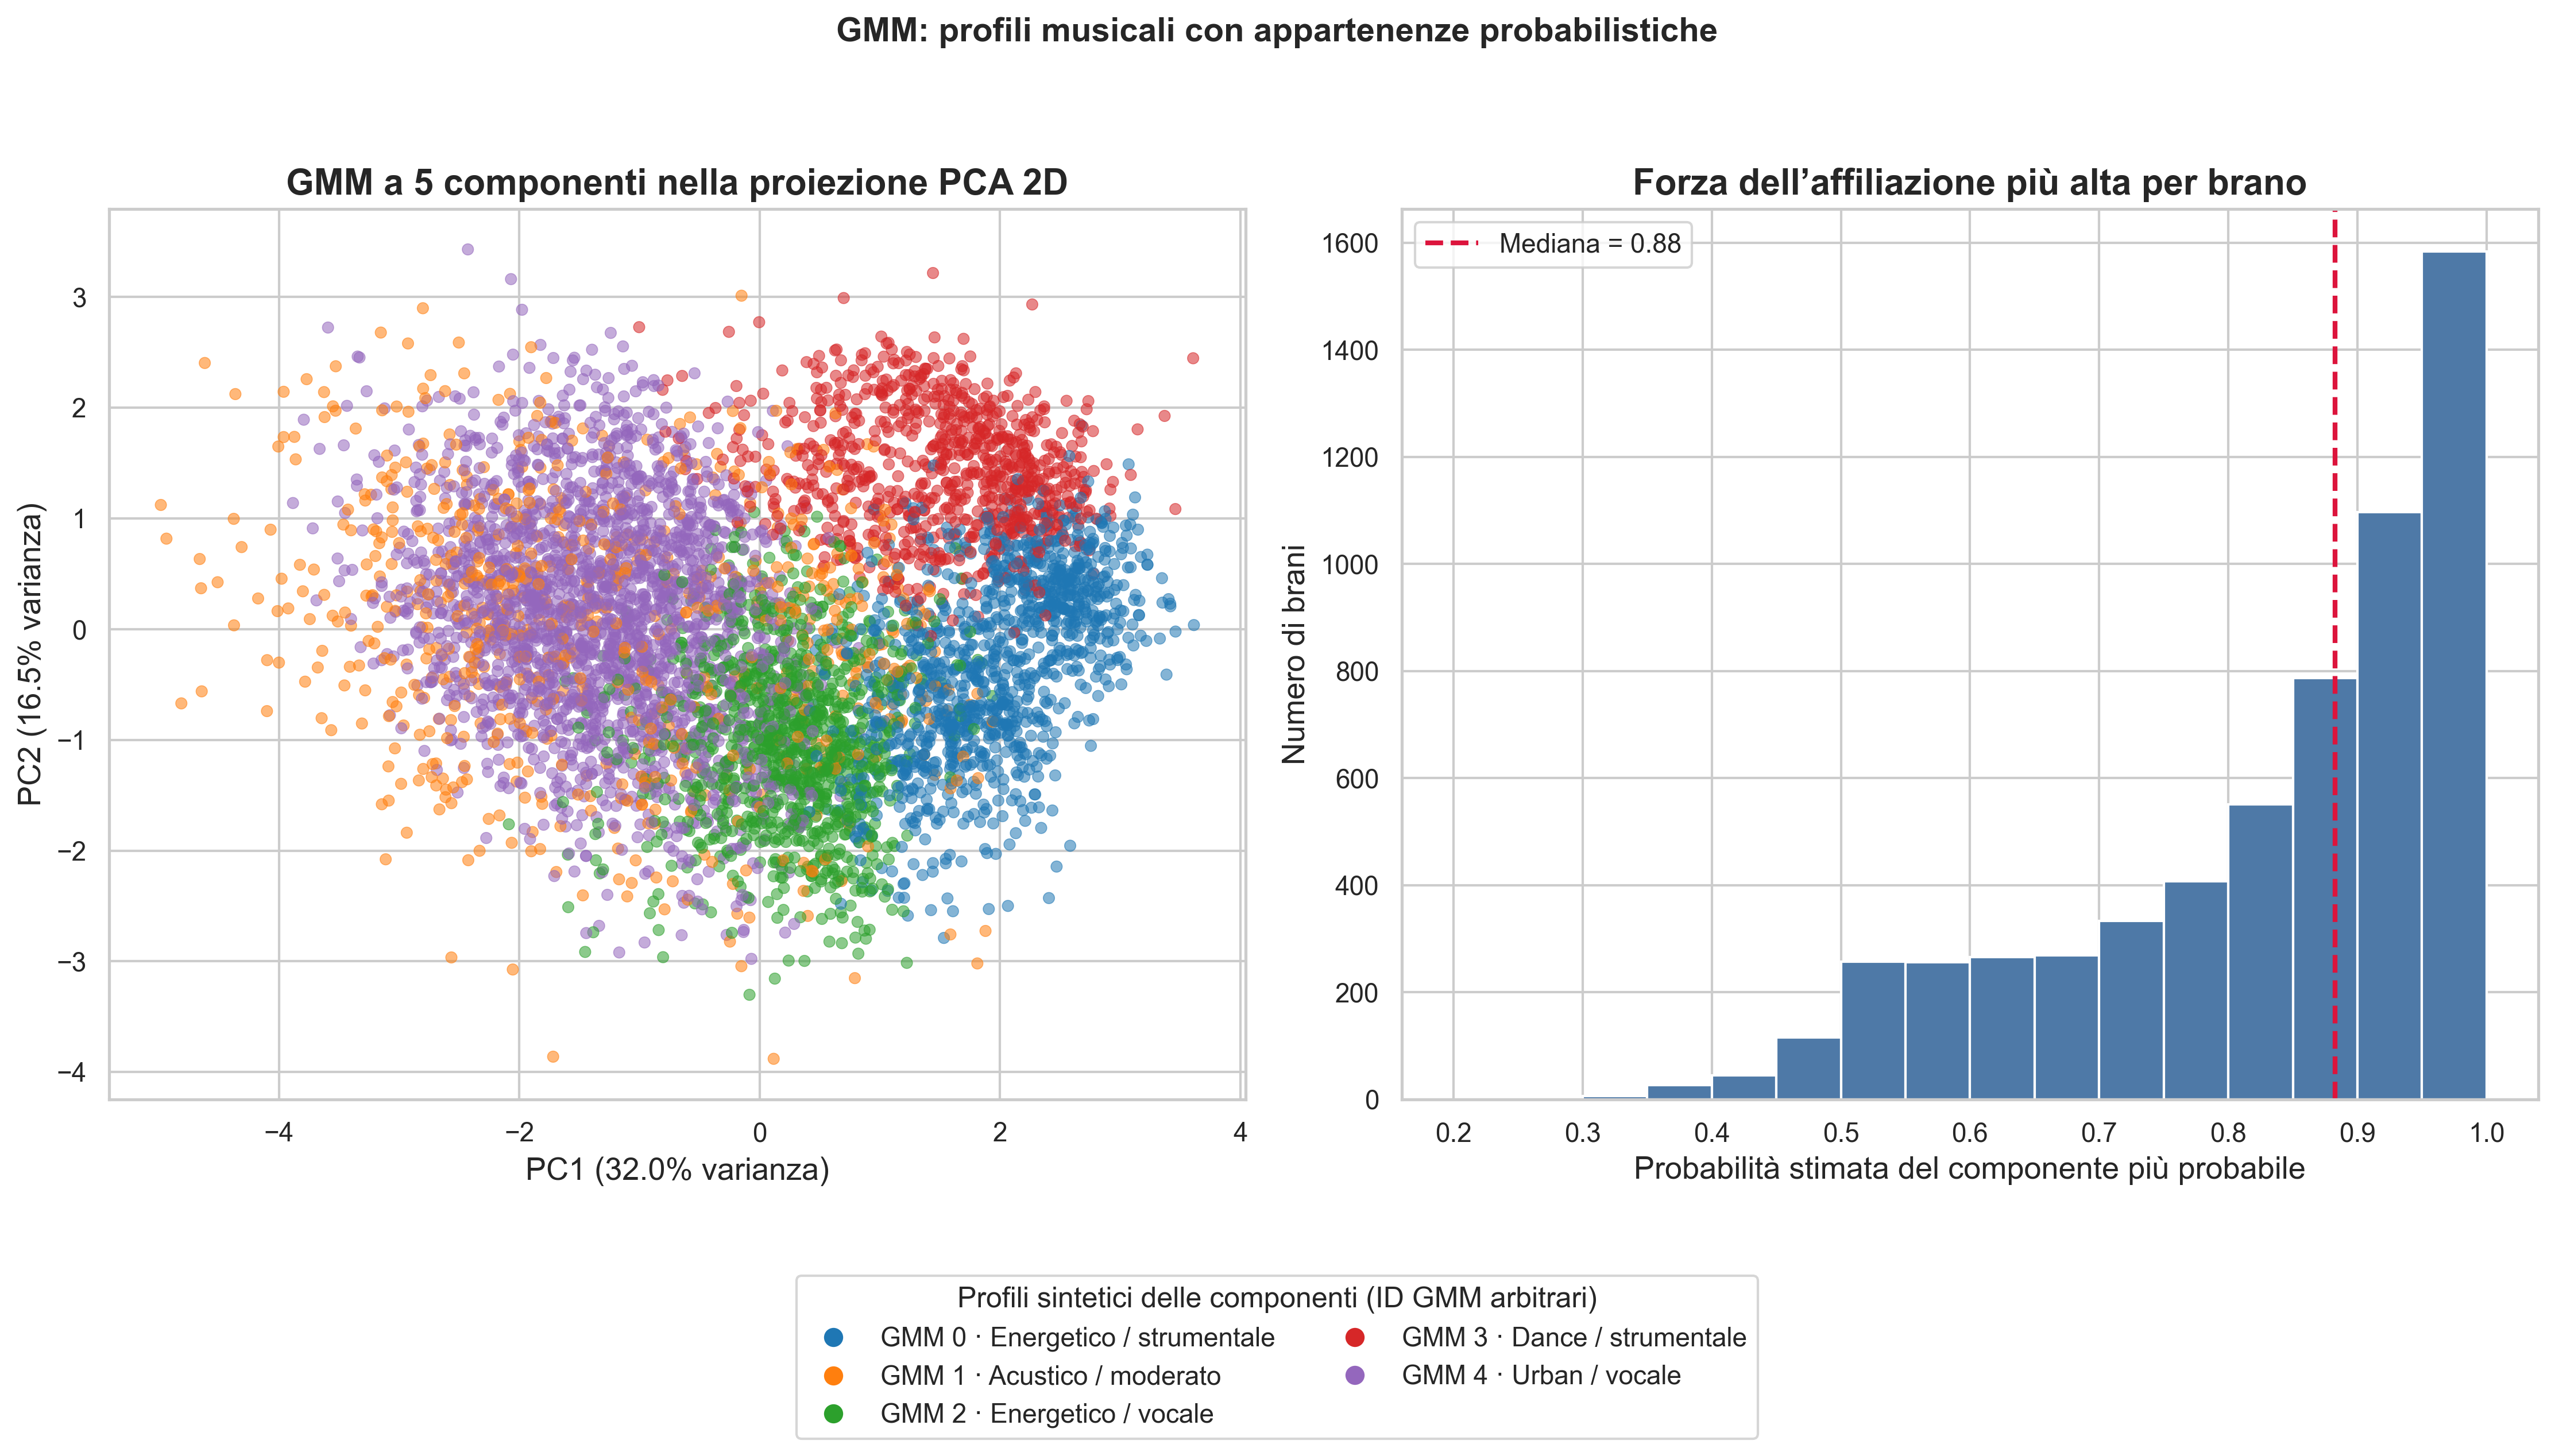
\includegraphics[width=\textwidth]{capitolo4/img/fig24_gmm_soft_membership.png}
    \caption{Mappa topografica GMM nello spazio PCA 2D con ellissi di dispersione ($1\sigma$ continua, $2\sigma$ tratteggiata) ed evidenziazione dei 409 brani ponte cross-mood (a sinistra), affiancata dalla graduatoria dei corridoi ibridi più frequenti (a destra).}
    \label{fig:gmm_soft}
\end{figure}

Per tradurre intuitivamente la complessa interazione probabilistica a 5 dimensioni, la Figura \ref{fig:gmm_radviz} introduce il \textbf{Pentagono Baricentrico dei Mood (RadViz Simplex Plot)}. I 5 vertici del pentagono rappresentano gli archetipi "puri" ($\gamma_{i,k} = 1$); ciascun brano viene posizionato nel piano mediante la combinazione lineare convessa dei vettori dei vertici pesata sulle rispettive probabilità:
\begin{equation}
\mathbf{P}_i = \sum_{k=0}^4 \gamma_{i,k} \, \mathbf{V}_k
\label{eq:radviz_simplex}
\end{equation}
I cerchi concentrici indicano il grado di purezza dell'affiliazione ($50\%$, $75\%$, $100\%$). I brani stilisticamente stereotipati vengono attratti verso la periferia lungo i raggi dei singoli poli, mentre i brani ibridi galleggiano verso il baricentro o lungo i segmenti perimetrali che collegano due mood specifici.

\begin{figure}[H]
    \centering
    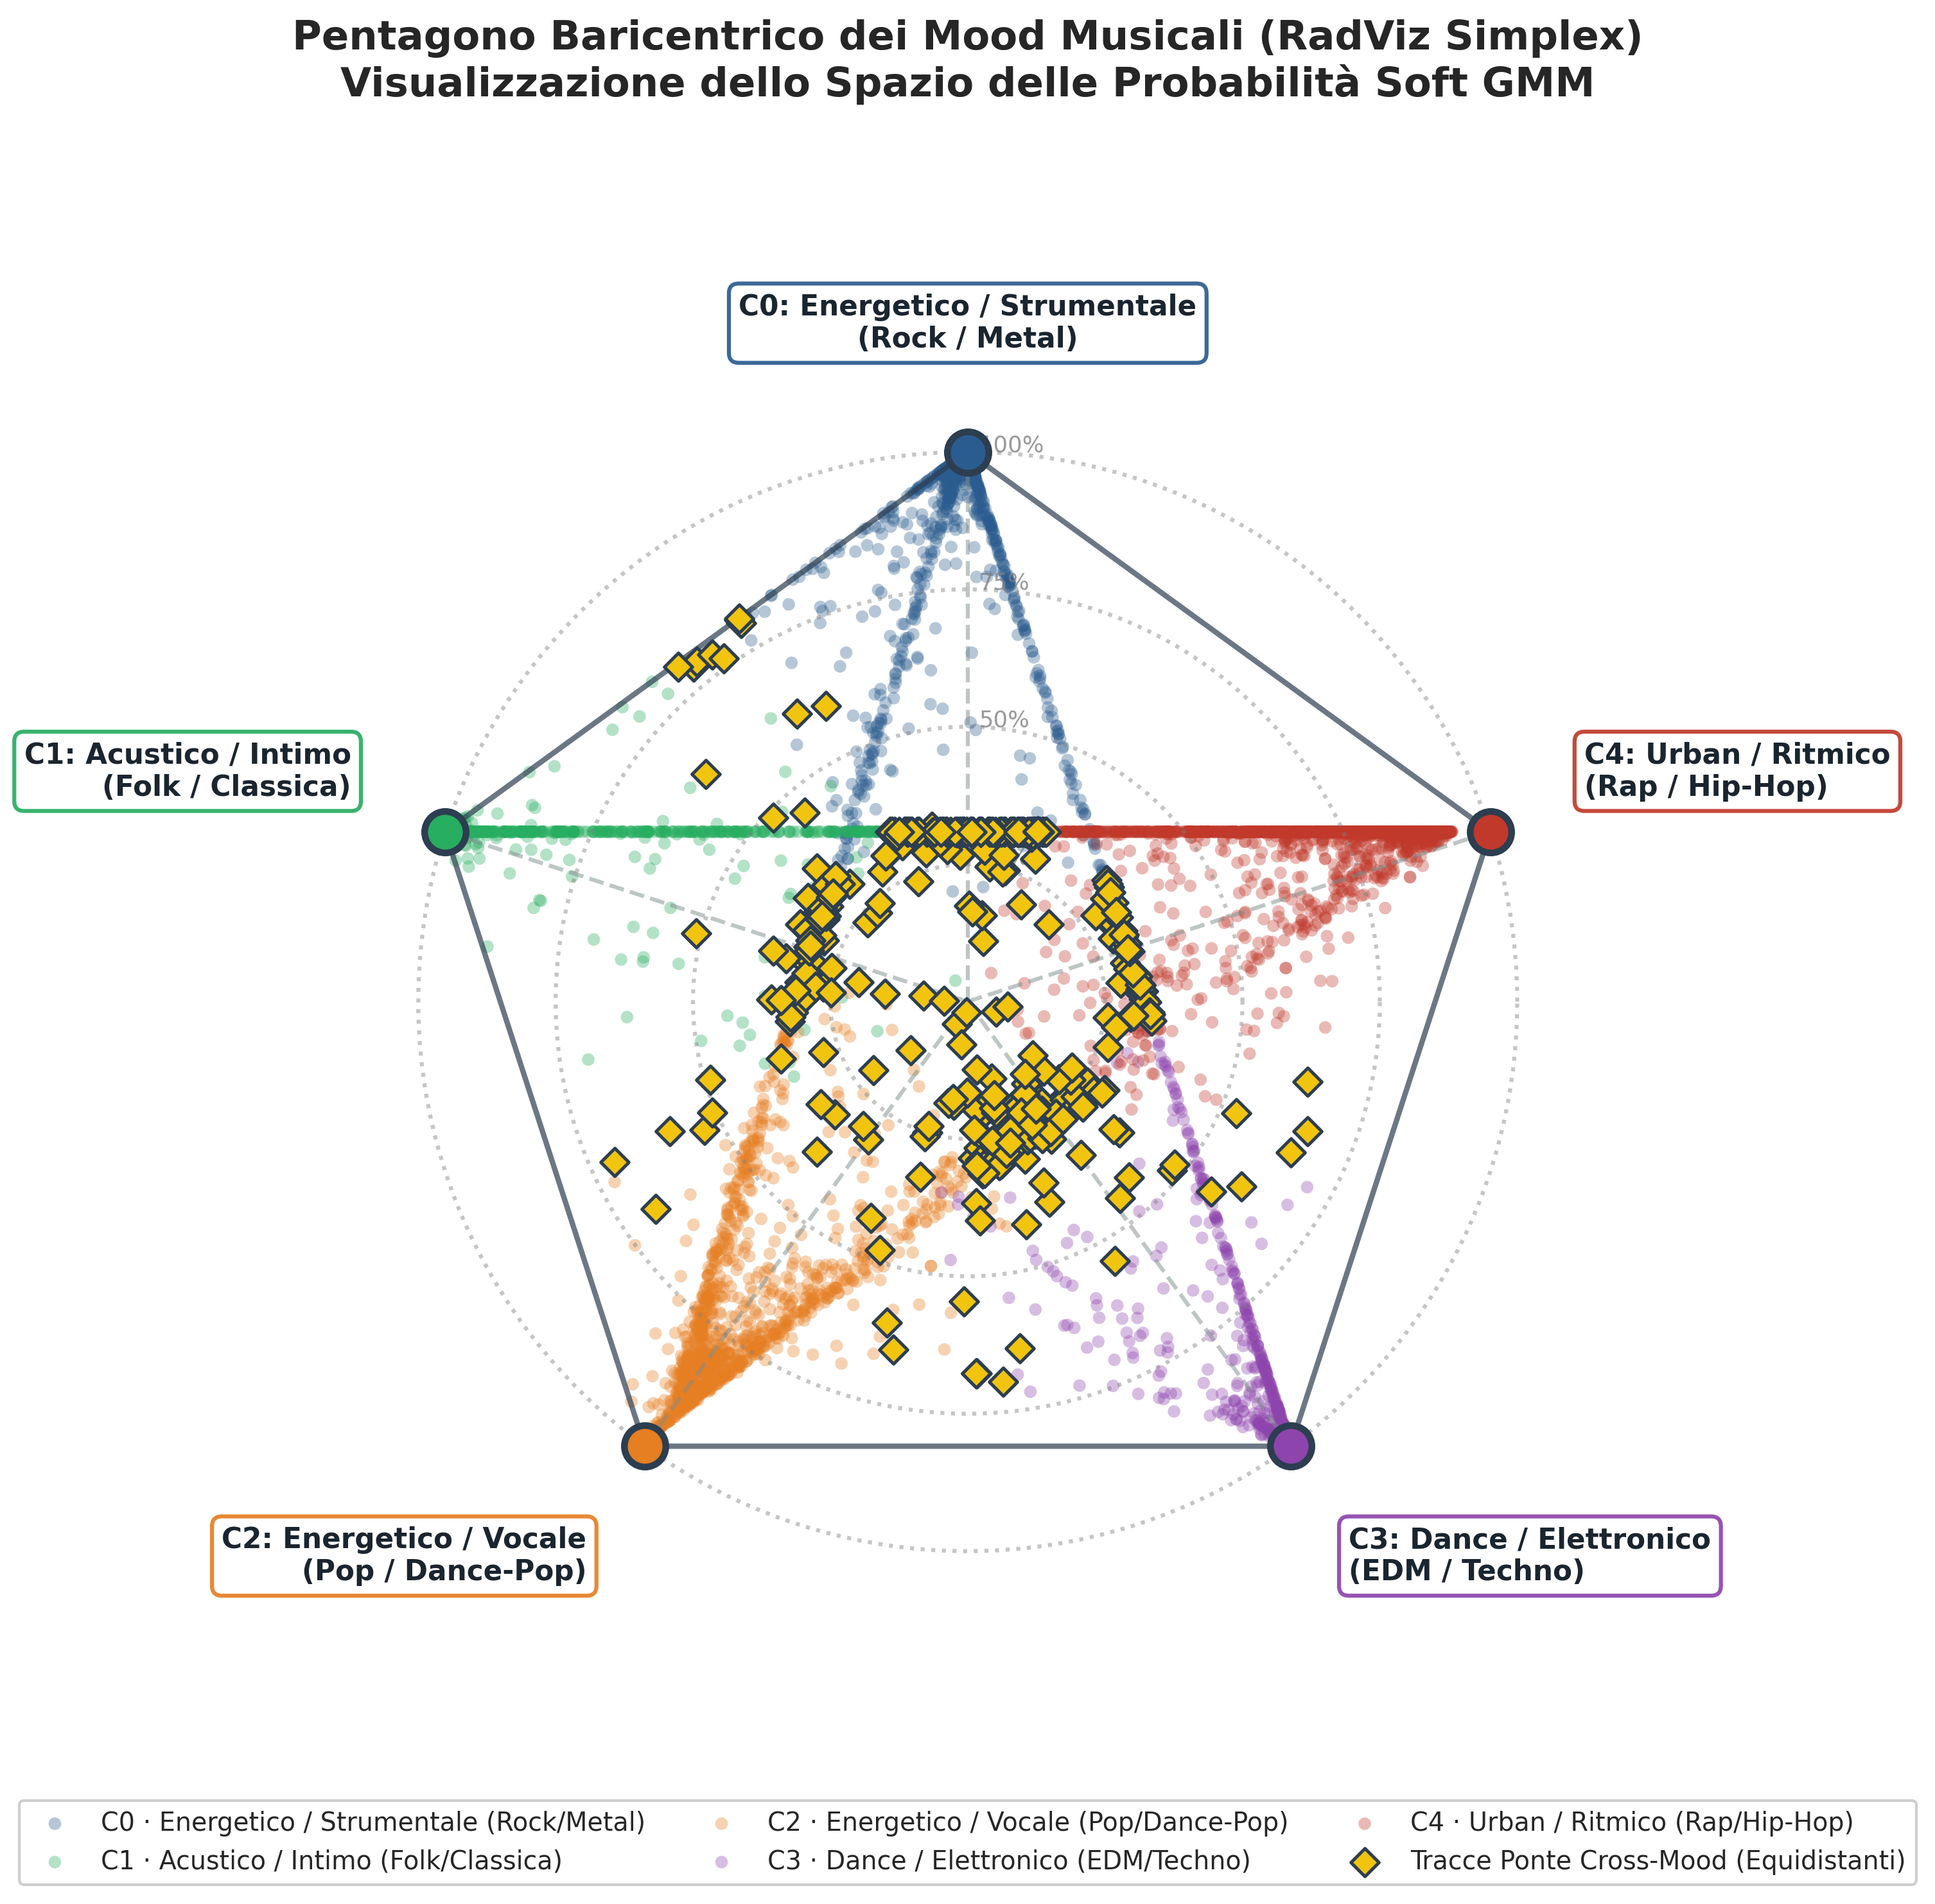
\includegraphics[width=0.82\textwidth]{capitolo4/img/fig24b_mood_pentagon_radviz.png}
    \caption{Pentagono Baricentrico dei Mood (RadViz Simplex Plot): visualizzazione dello spazio delle probabilità soft GMM con cerchi guida di confidenza e posizionamento delle tracce ponte.}
    \label{fig:gmm_radviz}
\end{figure}

\paragraph{Identificazione dei Brani Ponte (Cross-Mood Bridge Tracks) ed Esempi Concreti:}
Fissando una soglia esplorativa di ambiguità metrica pari a $\text{Gap}_{\text{top2}} \le 0,15$ (differenza non superiore al 15\% tra le due massime probabilità a posteriori), il modello isola nel campione esattamente \textbf{409 brani ponte} (il \textbf{6,82\%} del catalogo), con un'affiliazione massima mediana complessiva pari a $0,883$. Come visibile nella Figura \ref{fig:gmm_soft}, questi brani non sono dispersi casualmente, ma si addensano con precisione matematica lungo le selle topografiche di sovrapposizione tra le campane gaussiane. 

L'ispezione analitica dei singoli brani estratti dal dataset conferma la straordinaria corrispondenza tra geometria del modello e percezione musicale:
\begin{itemize}
    \item Il brano \textit{"LostInMyhead"} (catalogato commercialmente come \textit{Dark Trap}) si colloca in perfetto equilibrio tra la Componente 1 (\textit{Acustico / Intimo}, $\gamma_1 = 50,5\%$) e la Componente 4 (\textit{Urban / Ritmico}, $\gamma_4 = 49,5\%$), con un gap di appena l'$1,0\%$. La traccia unisce un arpeggio lo-fi rarefatto a una linea di basso hip-hop cadenzata.
    \item Il brano \textit{"Cool Girl"} (etichettato come \textit{Pop}) fa da ponte tra la Componente 1 ($\gamma_1 = 52,3\%$) e la Componente 4 ($\gamma_4 = 47,7\%$, gap $4,5\%$), combinando una produzione radiofonica brillante con una strofa ritmata a cavallo tra melodia e parlato.
    \item La traccia \textit{"Abstergence"} costituisce un caso emblematico di ponte a tre vie, distribuendosi tra la Componente 3 (\textit{Dance / Elettronico}, $41,9\%$), la Componente 2 (\textit{Energetico / Vocale}, $31,4\%$) e la Componente 0 (\textit{Energetico / Strumentale}, $20,8\%$).
\end{itemize}

Dalla graduatoria dei corridoi ibridi in Figura \ref{fig:gmm_soft} emerge che le transizioni più frequenti avvengono tra l'archetipo acustico e quello urban ($C_1 \leftrightarrow C_4$: 149 brani), seguiti dal raccordo tra pop vocale e urban ($C_2 \leftrightarrow C_4$: 102 brani) e tra rock/metal e pop energico ($C_0 \leftrightarrow C_2$: 51 brani). Questa proprietà abilita una concreta applicazione industriale per i servizi di streaming: la generazione di \textbf{Playlist di Transizione Dinamica} (\textit{Cross-Mood Fade-in}), capaci di condurre l'ascoltatore da una sessione rilassante o acustica verso sonorità urban o clubbing attraverso brani cuscinetto timbricamente affini a entrambi i mondi.

\begin{table}[H]
\centering
\caption{Sintesi descrittiva delle componenti GMM sul campione di 6.000 brani. I generi sono riportati solo come interpretazione a posteriori.}
\label{tab:gmm_profile}
\vspace{0.2cm}
\small
\begin{tabularx}{\textwidth}{c r X X}
\toprule
\textbf{Componente} & \textbf{Brani} & \textbf{Tratti acustici medi distintivi} & \textbf{Generi più frequenti (a posteriori)} \\
\midrule
0 & 1.130 & Energia alta ($0,92$), strumentalità alta ($0,72$), durata lunga ($352$ s) & Psytrance, DnB, Trance \\
1 & 741 & Maggiore acusticità ($0,39$), energia più contenuta ($0,51$) & Dark Trap, Underground Rap, RnB \\
2 & 1.111 & Energia alta ($0,90$), prevalenza vocale ($\text{instrumentalness}=0,08$) & Hardstyle, Trap, Emo \\
3 & 843 & Ballabilità alta ($0,74$), strumentalità alta ($0,76$), durata lunga ($367$ s) & Techno, Techhouse \\
4 & 2.175 & Profilo più vocale ($\text{speechiness}=0,20$), ballabilità alta ($0,71$) & Underground Rap, Dark Trap, Hiphop \\
\bottomrule
\end{tabularx}
\end{table}

Le componenti 0 e 3, ad esempio, condividono una forte componente strumentale ma si distinguono per intensità e ballabilità; le componenti 1, 2 e 4 separano ulteriormente profili acustici o vocali. La numerazione delle componenti è arbitraria e non costituisce una gerarchia di mood.

\newpage
\subsection{DBSCAN nello Spazio PCA}

DBSCAN (\textit{Density-Based Spatial Clustering of Applications with Noise}) è un algoritmo di clustering basato sulla densità locale dei punti nello spazio metrico. A differenza di K-Means (che assegna ogni brano a un centroide), DBSCAN non richiede di fissare a priori il numero di cluster e marca come \textbf{noise} (etichetta $-1$) i punti che non soddisfano i criteri di densità locale. Questa etichetta descrive la geometria rispetto al modello e ai parametri scelti; non è un giudizio sul valore musicale della traccia.

Il comportamento di DBSCAN nello spazio PCA a 4 dimensioni dipende da due iperparametri:
\begin{itemize}
    \item $\epsilon$ (\textit{epsilon}): il raggio dell'ipersfera quadridimensionale entro cui ricercare i vicini di ciascun brano;
    \item \texttt{min\_samples}: il numero minimo di brani richiesti entro il raggio $\epsilon$ affinché un'osservazione sia qualificata come \textit{punto core}.
\end{itemize}

\subsubsection{Scelta dei parametri e tuning nello spazio PCA}

Per calibrare il raggio $\epsilon$ sulla scala metrica delle 4 Componenti Principali, è stato applicato il metodo delle distanze $k$-Nearest Neighbors ($k$-NN) con $k = \texttt{min\_samples} = 5$ (Figura \ref{fig:dbscan_knn}), affiancato da una ricerca su griglia bidimensionale $(\epsilon \in \{0,45; 0,50; 0,60; 0,70\} \times \texttt{min\_samples} \in \{4, 5, 6, 8\})$ volta a monitorare simultaneamente il numero di cluster generati e il Silhouette Score dei punti non rumorosi (Figura \ref{fig:dbscan_grid}).

\begin{figure}[H]
    \centering
    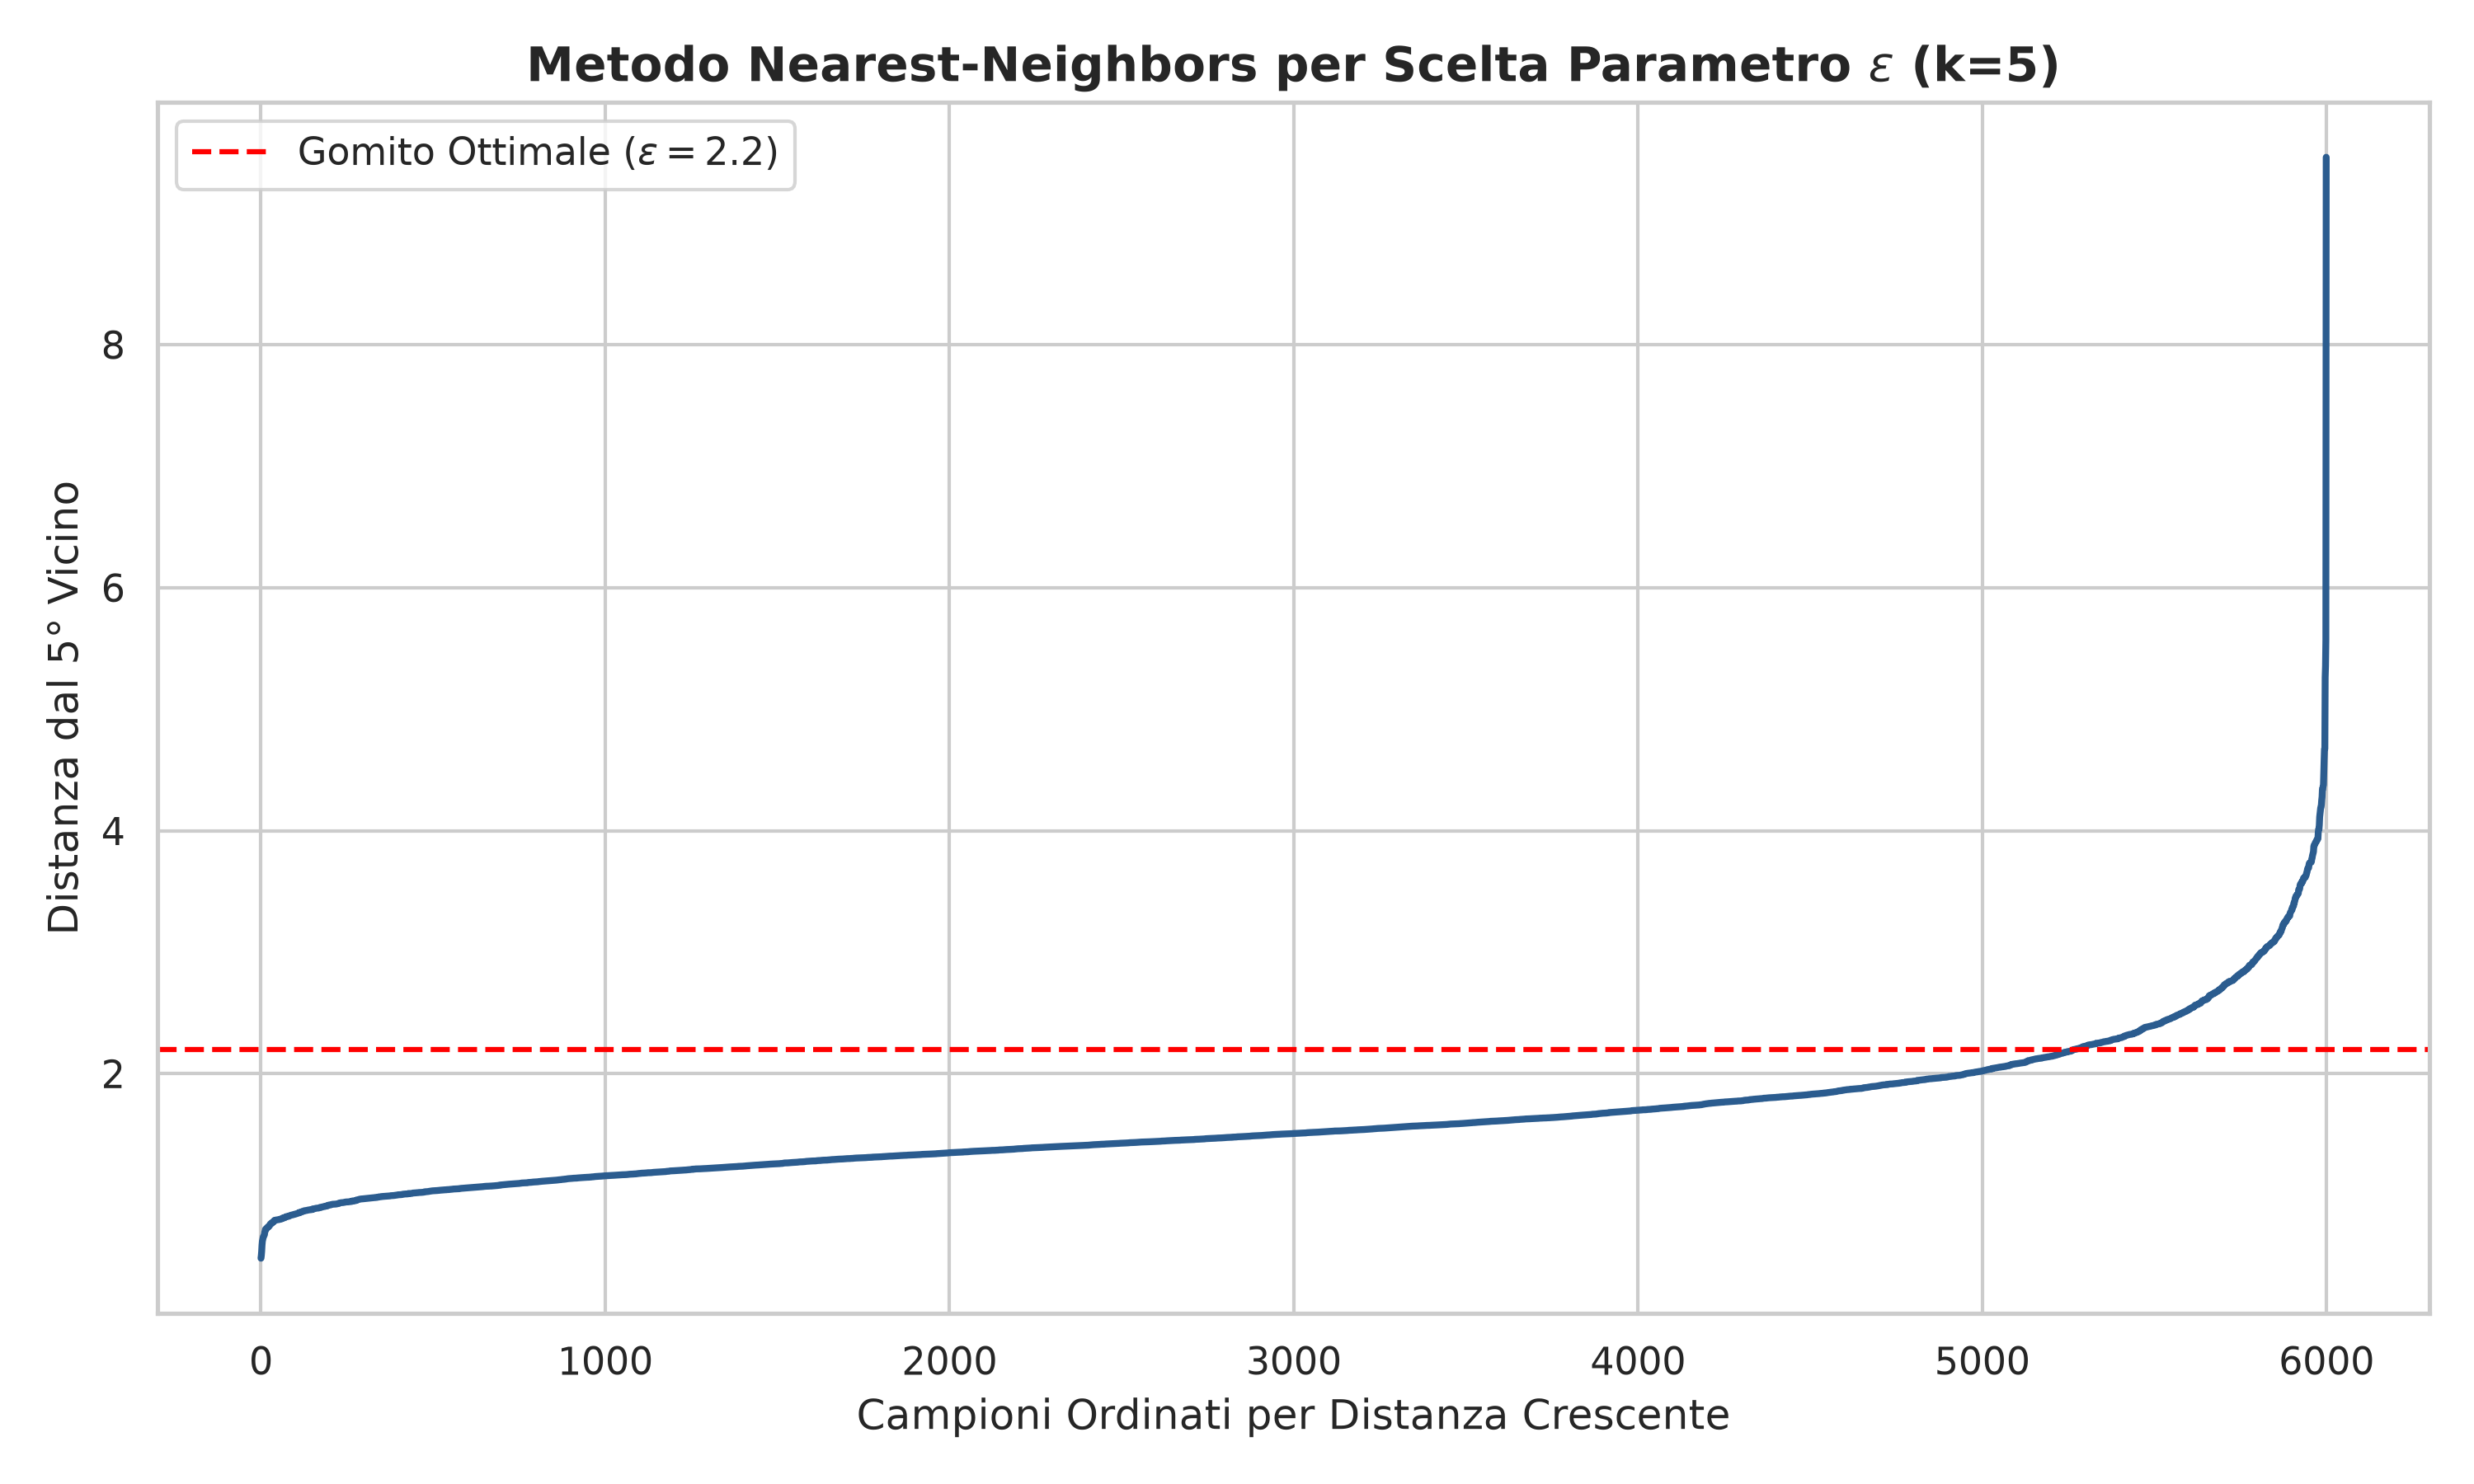
\includegraphics[width=0.76\textwidth]{capitolo4/img/fig20_dbscan_knn_distance.png}
    \caption{Curva ordinata delle distanze dal 5° vicino più prossimo ($k$-NN) nello spazio PCA a 4 componenti, con ginocchio ottimale in $\epsilon = 0,60$.}
    \label{fig:dbscan_knn}
\end{figure}

\begin{figure}[H]
    \centering
    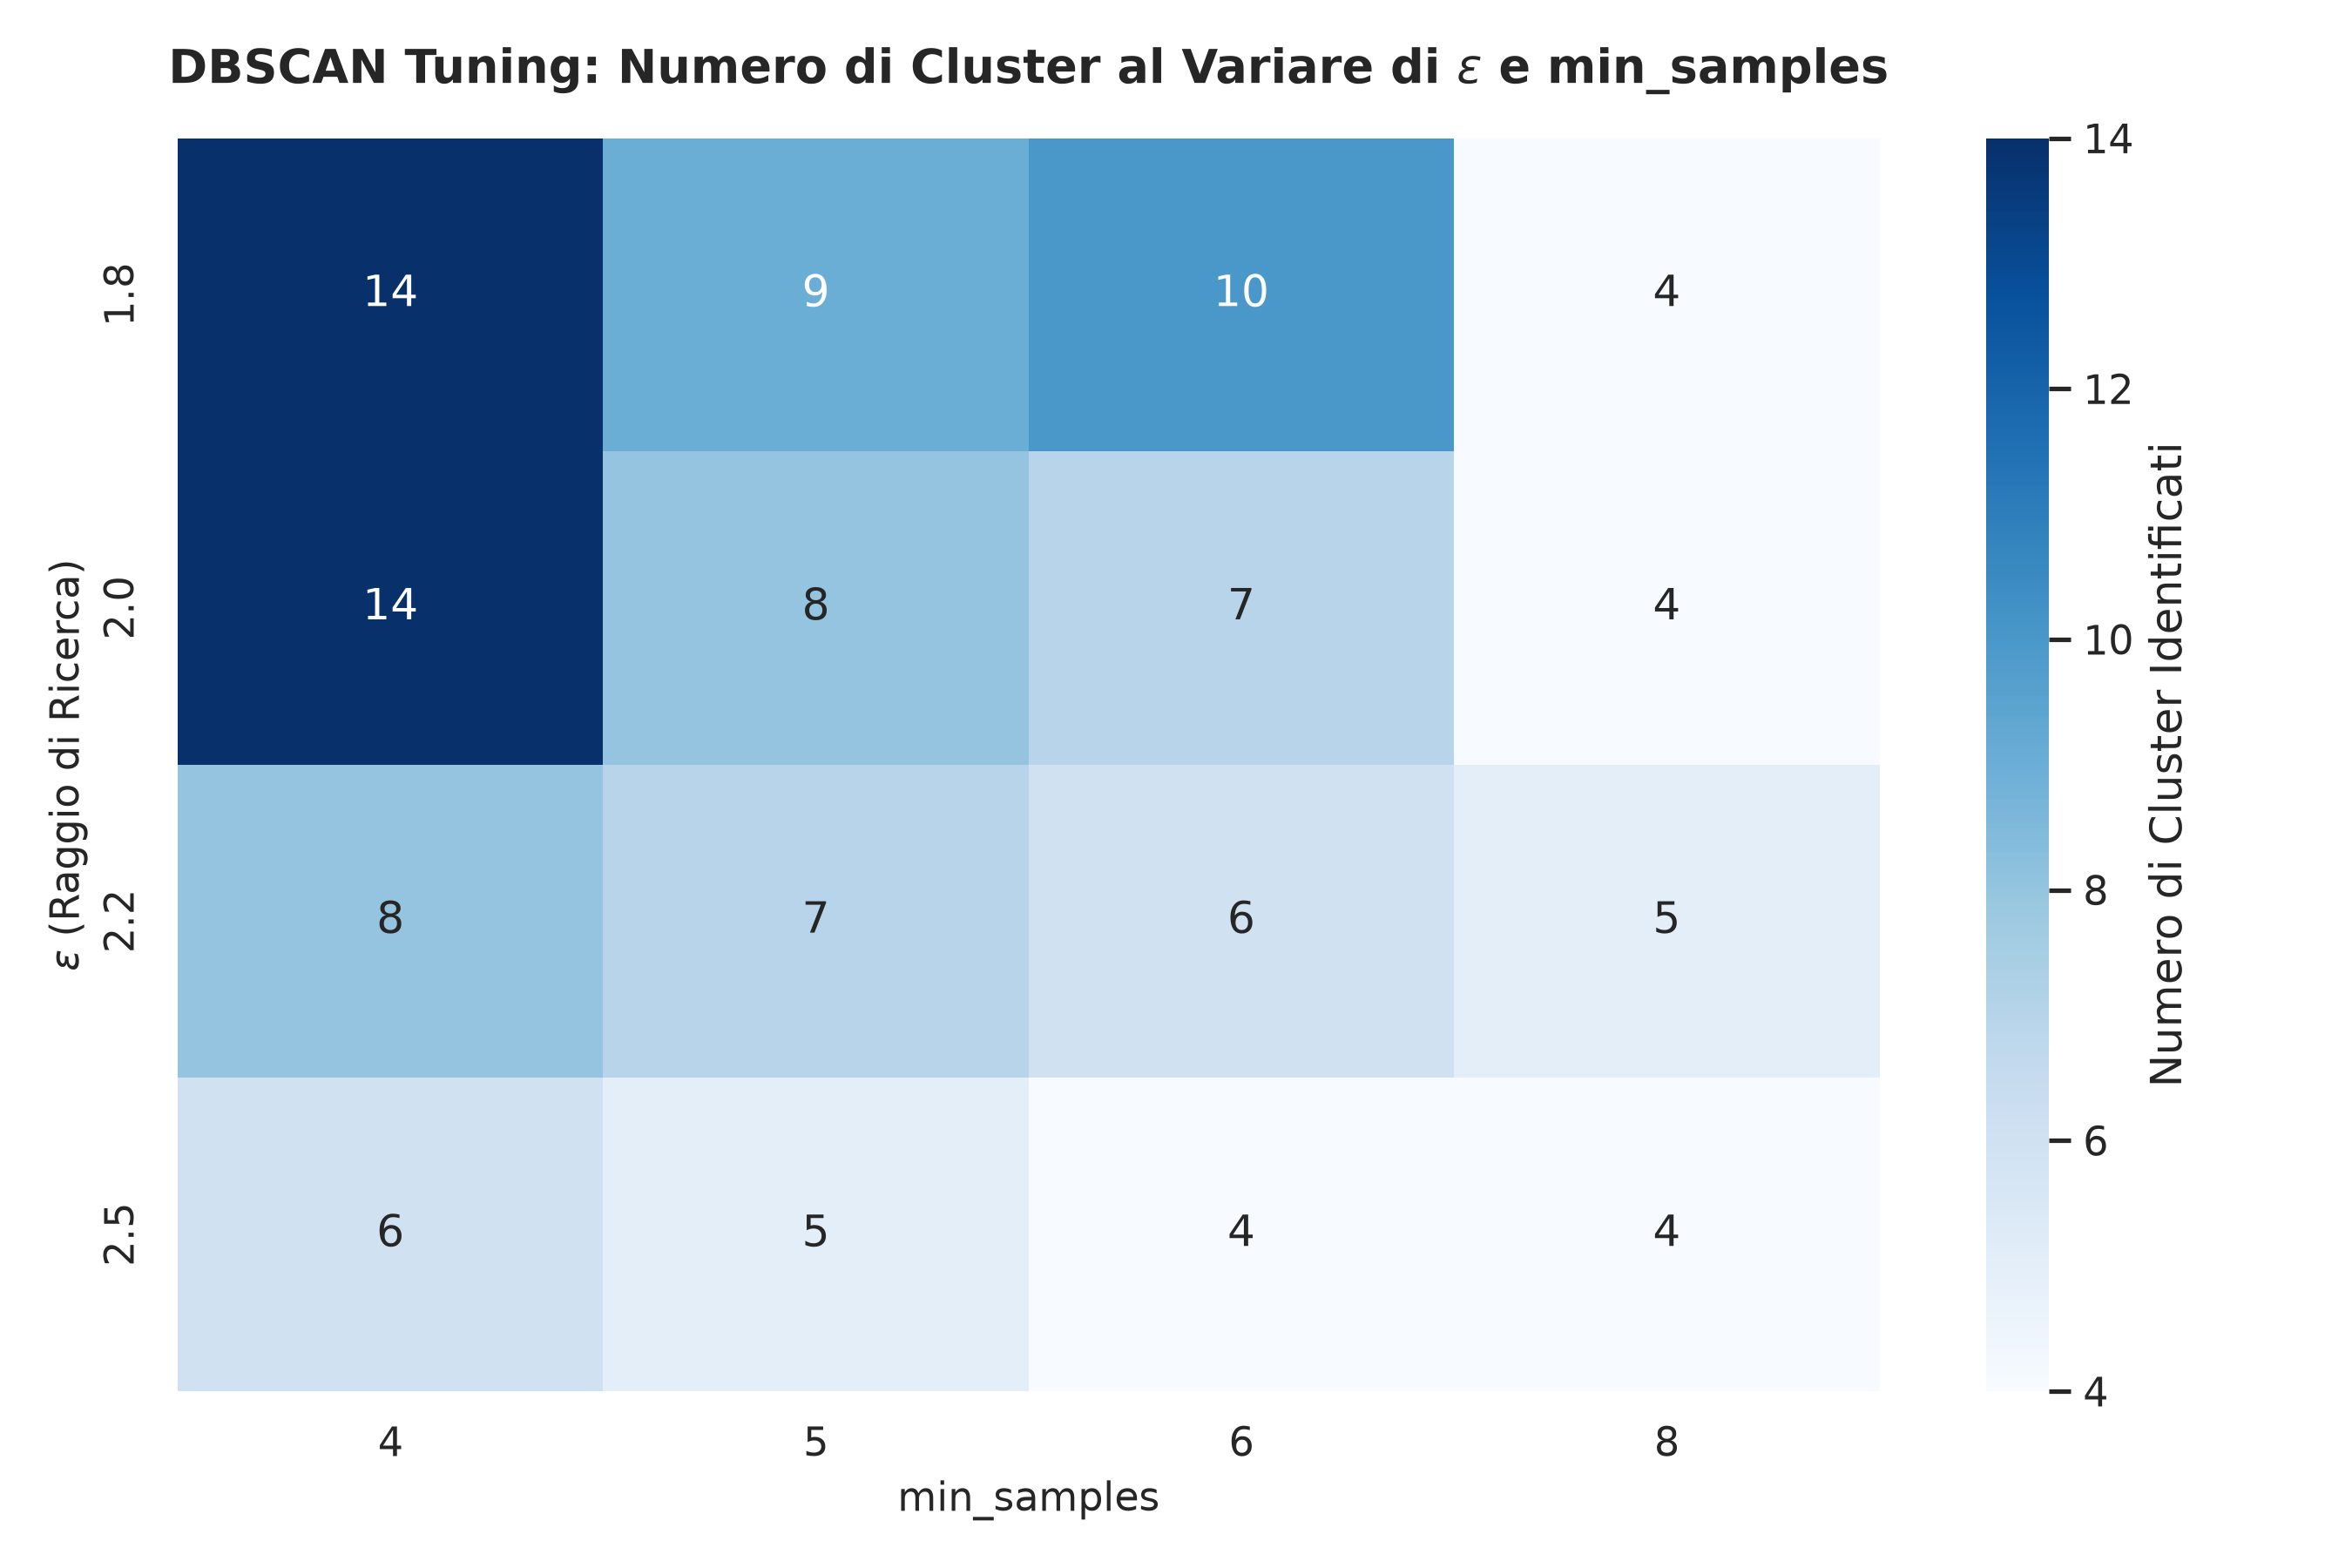
\includegraphics[width=0.95\textwidth]{capitolo4/img/fig21_dbscan_grid_search.png}
    \caption{Griglia di tuning iperparametrica DBSCAN nello spazio PCA 4D: Numero di cluster identificati (a sinistra) e Silhouette Score dei punti assegnati (a destra).}
    \label{fig:dbscan_grid}
\end{figure}

L'ispezione della curva $k$-NN (Figura \ref{fig:dbscan_knn}) evidenzia che le distanze dal 5° vicino si mantengono contenute sotto $0,55$ per oltre il 90\% del campione, per poi impennarsi bruscamente (il "gomito" della curva) intorno alla soglia \textbf{$\epsilon = 0,60$}. Dalla griglia di Figura \ref{fig:dbscan_grid} si osserva che:
\begin{itemize}
    \item Valori di raggio troppo piccoli ($\epsilon = 0,45$) causano una sovra-frammentazione della coda della distribuzione ($20\text{--}27$ micro-cluster) ed espellono oltre il 20\% del catalogo come rumore.
    \item In corrispondenza del punto di gomito \textbf{$\epsilon = 0,60, \texttt{min\_samples} = 5$}, l'algoritmo identifica \textbf{6 cluster} e marca come noise \textbf{462 brani} (\textbf{7,70\% del campione}). La Silhouette sui punti assegnati è $0,120$; con $\texttt{min\_samples}=8$ sale a $0,332$, ma rimangono 3 cluster e la quota noise cresce all'11,05\%.
\end{itemize}

\newpage
\subsubsection{Analisi dei risultati ottenuti e interpretazione topologica}

La Figura \ref{fig:dbscan_tsne} mostra il risultato della clusterizzazione DBSCAN ($\epsilon = 0,60, \texttt{min\_samples} = 5$) proiettato sia sul piano lineare delle prime due Componenti Principali ($\text{PC}_1$ vs $\text{PC}_2$) sia sulla mappa non lineare t-SNE, evidenziando con croci rosse i 462 brani classificati come noise ($\text{label} = -1$).

\begin{figure}[H]
    \centering
    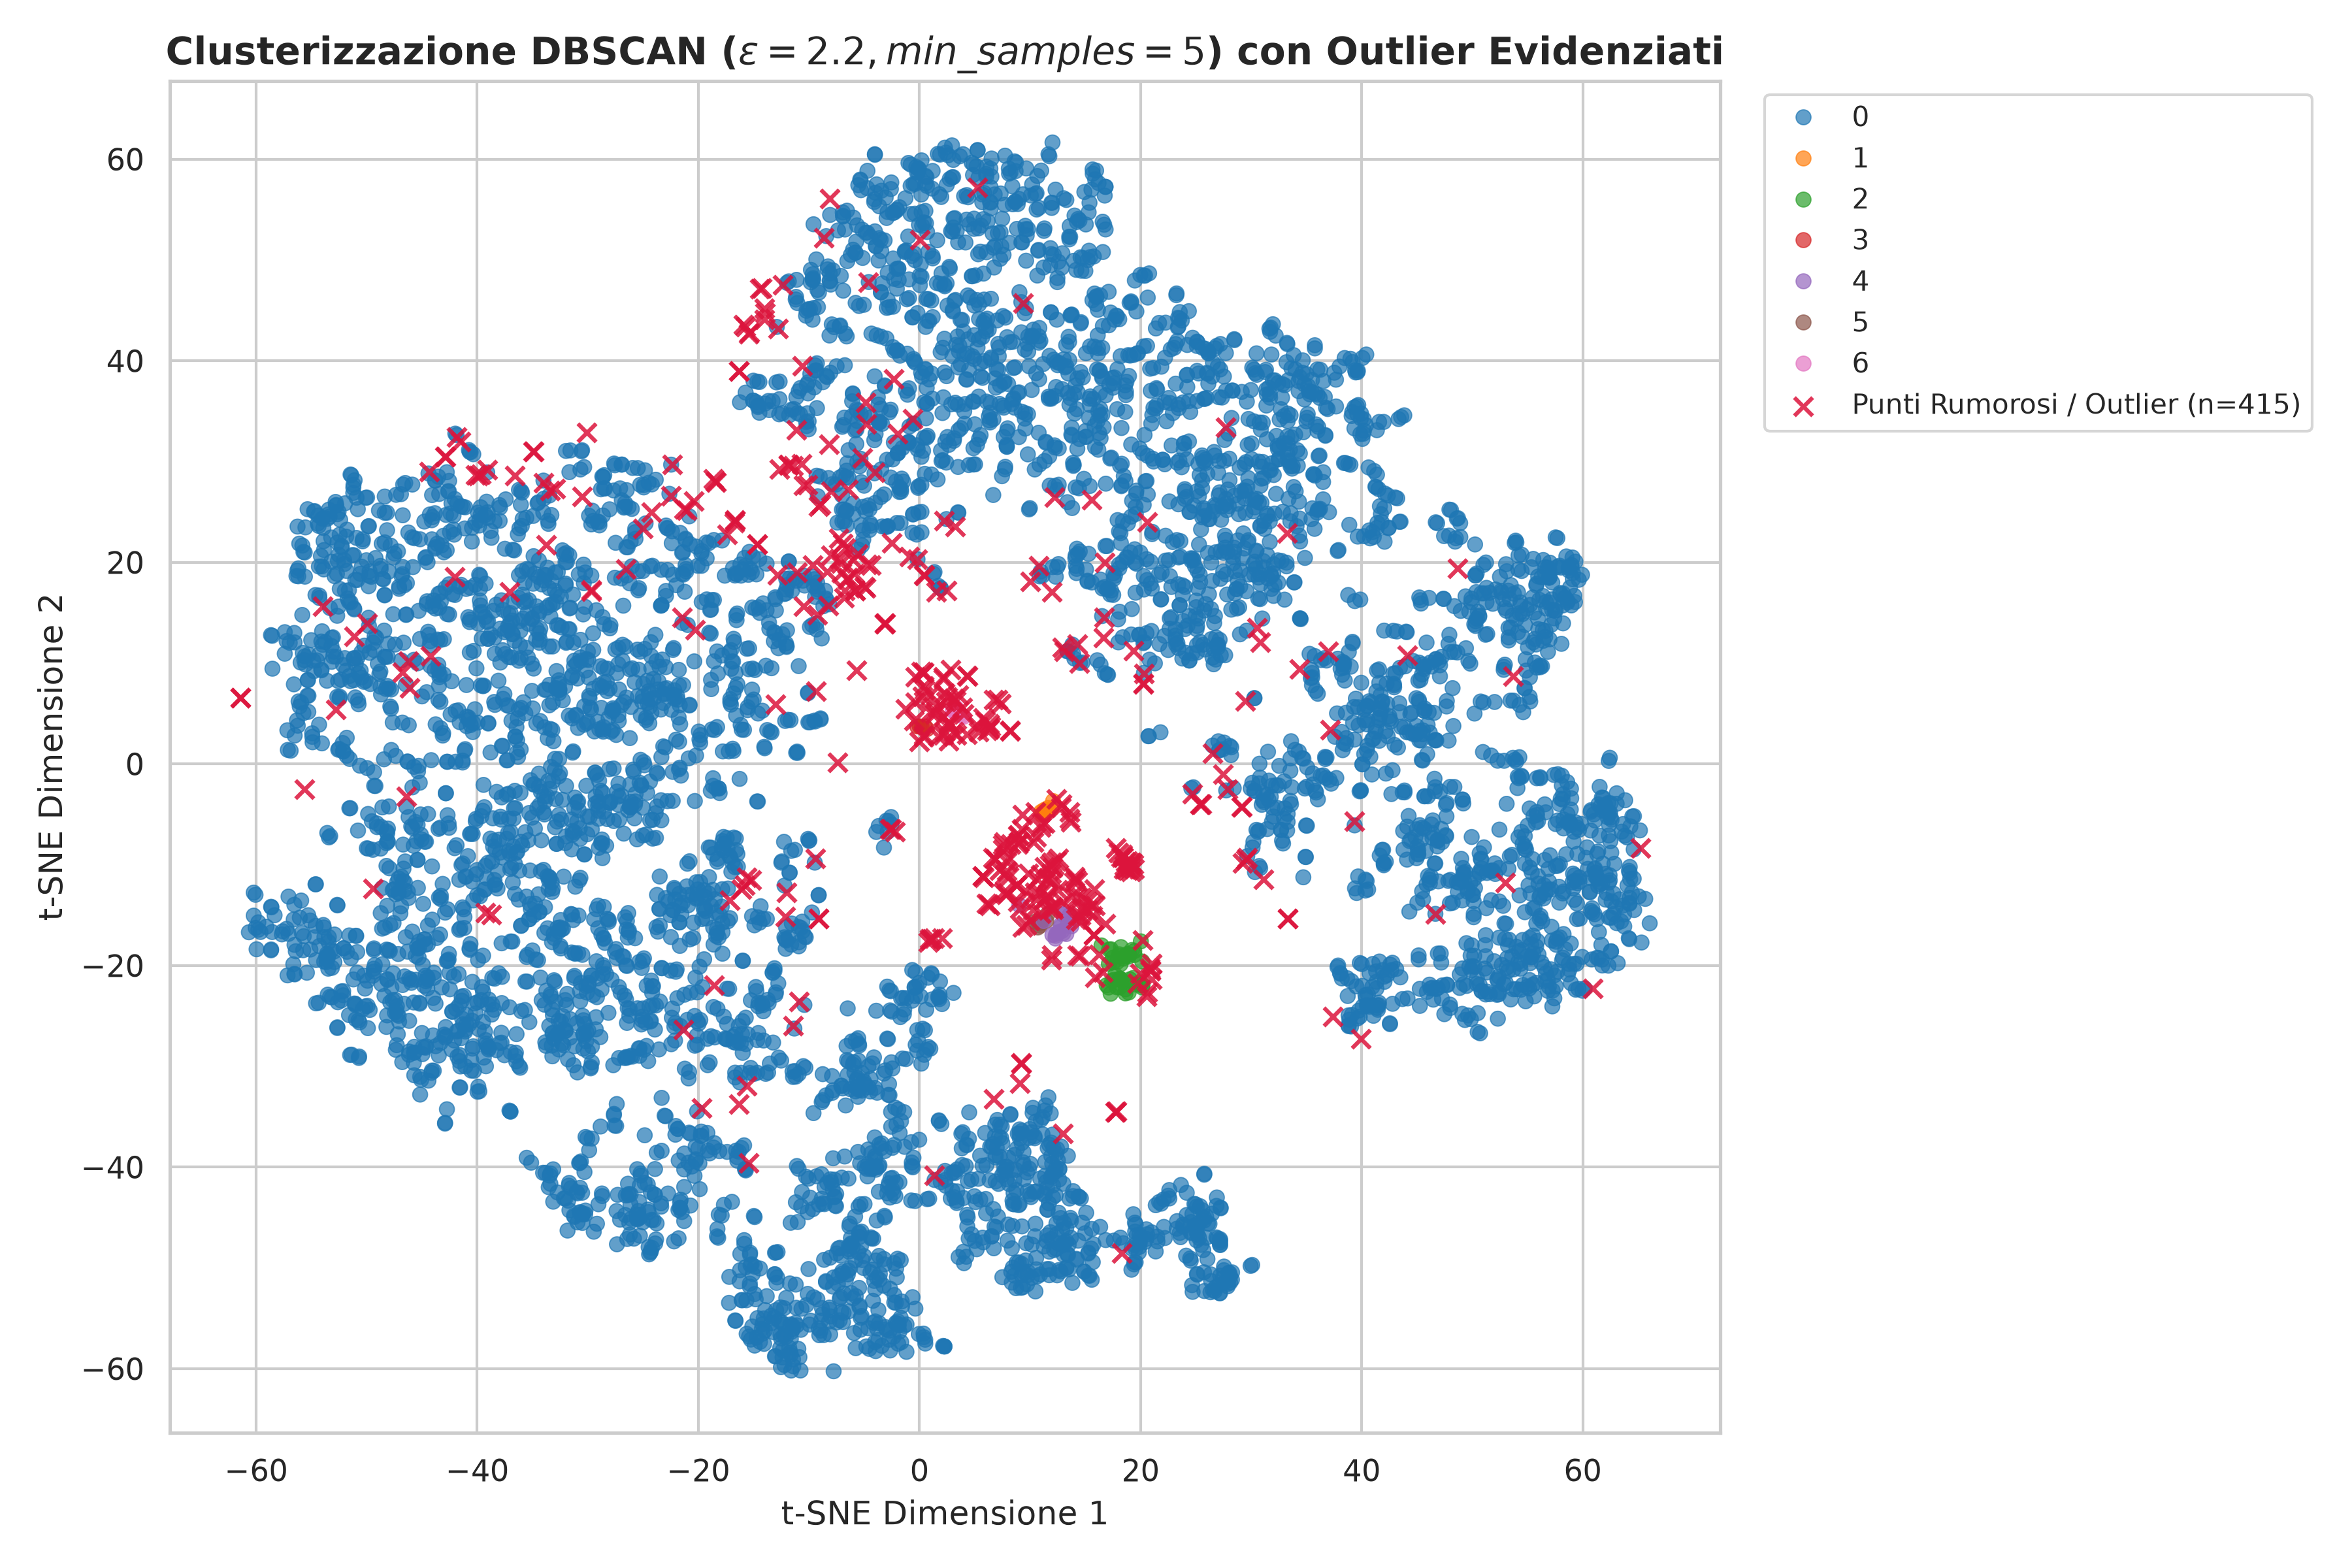
\includegraphics[width=0.96\textwidth]{capitolo4/img/fig22_dbscan_tsne_clusters_noise.png}
    \caption{Clusterizzazione DBSCAN ($\epsilon=0,60, \texttt{min\_samples}=5$) nello spazio PCA 2D (a sinistra) e t-SNE 2D (a destra), con evidenziazione dei 462 punti noise.}
    \label{fig:dbscan_tsne}
\end{figure}

Un'analisi oggettiva della Figura \ref{fig:dbscan_tsne} mette in luce un fenomeno topologico classico dei grandi cataloghi musicali:
\begin{itemize}
    \item \textbf{La "Megalopoli" Continua del Mainstream:} Le caratteristiche acustiche delle tracce pop, dance, urban ed elettroniche commerciali non presentano barriere geometriche nette né vuoti di densità nello spazio metrizzato, ma sfumano le une nelle altre lungo un continuum compatto. Di conseguenza, operando con una metrica rigida a raggio costante ($\epsilon = 0,60$), DBSCAN non intercetta interruzioni di continuità e connette la quasi totalità dell'universo musicale in un \textbf{unico macro-cluster dominante (Cluster 0, forte di $5.509$ brani, pari al $91,8\%$ del campione)}, affiancato da appena \textbf{5 micro-isole locali} ($29$ brani complessivi confinati su nicchie timbriche estreme).
    \item \textbf{La "Corona" Periferica a Bassa Densità:} L'algoritmo isola all'esterno una corona di \textbf{$462$ brani classificati come noise ($\text{label} = -1$, il $7,70\%$ del campione)}. Essi non soddisfano la condizione di avere almeno 5 vicini entro il raggio $\epsilon=0,60$.
\end{itemize}
Mentre K-Means forza geometricamente ogni osservazione entro uno dei cinque compartimenti, DBSCAN separa con rigore il nucleo compatto del catalogo dalle sue periferie metriche.

\subsubsection{Diagnostica del Rumore: la Rivalutazione Musicale dei Brani Periferici}

Per comprendere la natura acustica dei 462 brani etichettati come rumore ($\text{label} = -1$), la Figura \ref{fig:dbscan_noise} supera la sintesi schematica dei boxplot convenzionali introducendo un \textbf{Raincloud Plot} su tre variabili cardine: durata della traccia in minuti (\texttt{duration\_min}), contenuto verbale (\texttt{speechiness}) e timbrica acustica (\texttt{acousticness}). Il grafico integra simultaneamente tre livelli descrittivi:
\begin{enumerate}
    \item \textbf{Cloud (metà superiore):} Stima di densità continua non parametrica (Half-Violin KDE), che rivela la forma multimodale delle distribuzioni;
    \item \textbf{Boxplot (centro):} Sintesi robusta della mediana (marcatore circolare bianco) e dell'intervallo interquartile IQR;
    \item \textbf{Rain (metà inferiore):} Nuvola di dispersione con jitter dei singoli brani reali, che evidenzia la presenza e la concentrazione delle code estreme.
\end{enumerate}

\begin{figure}[H]
    \centering
    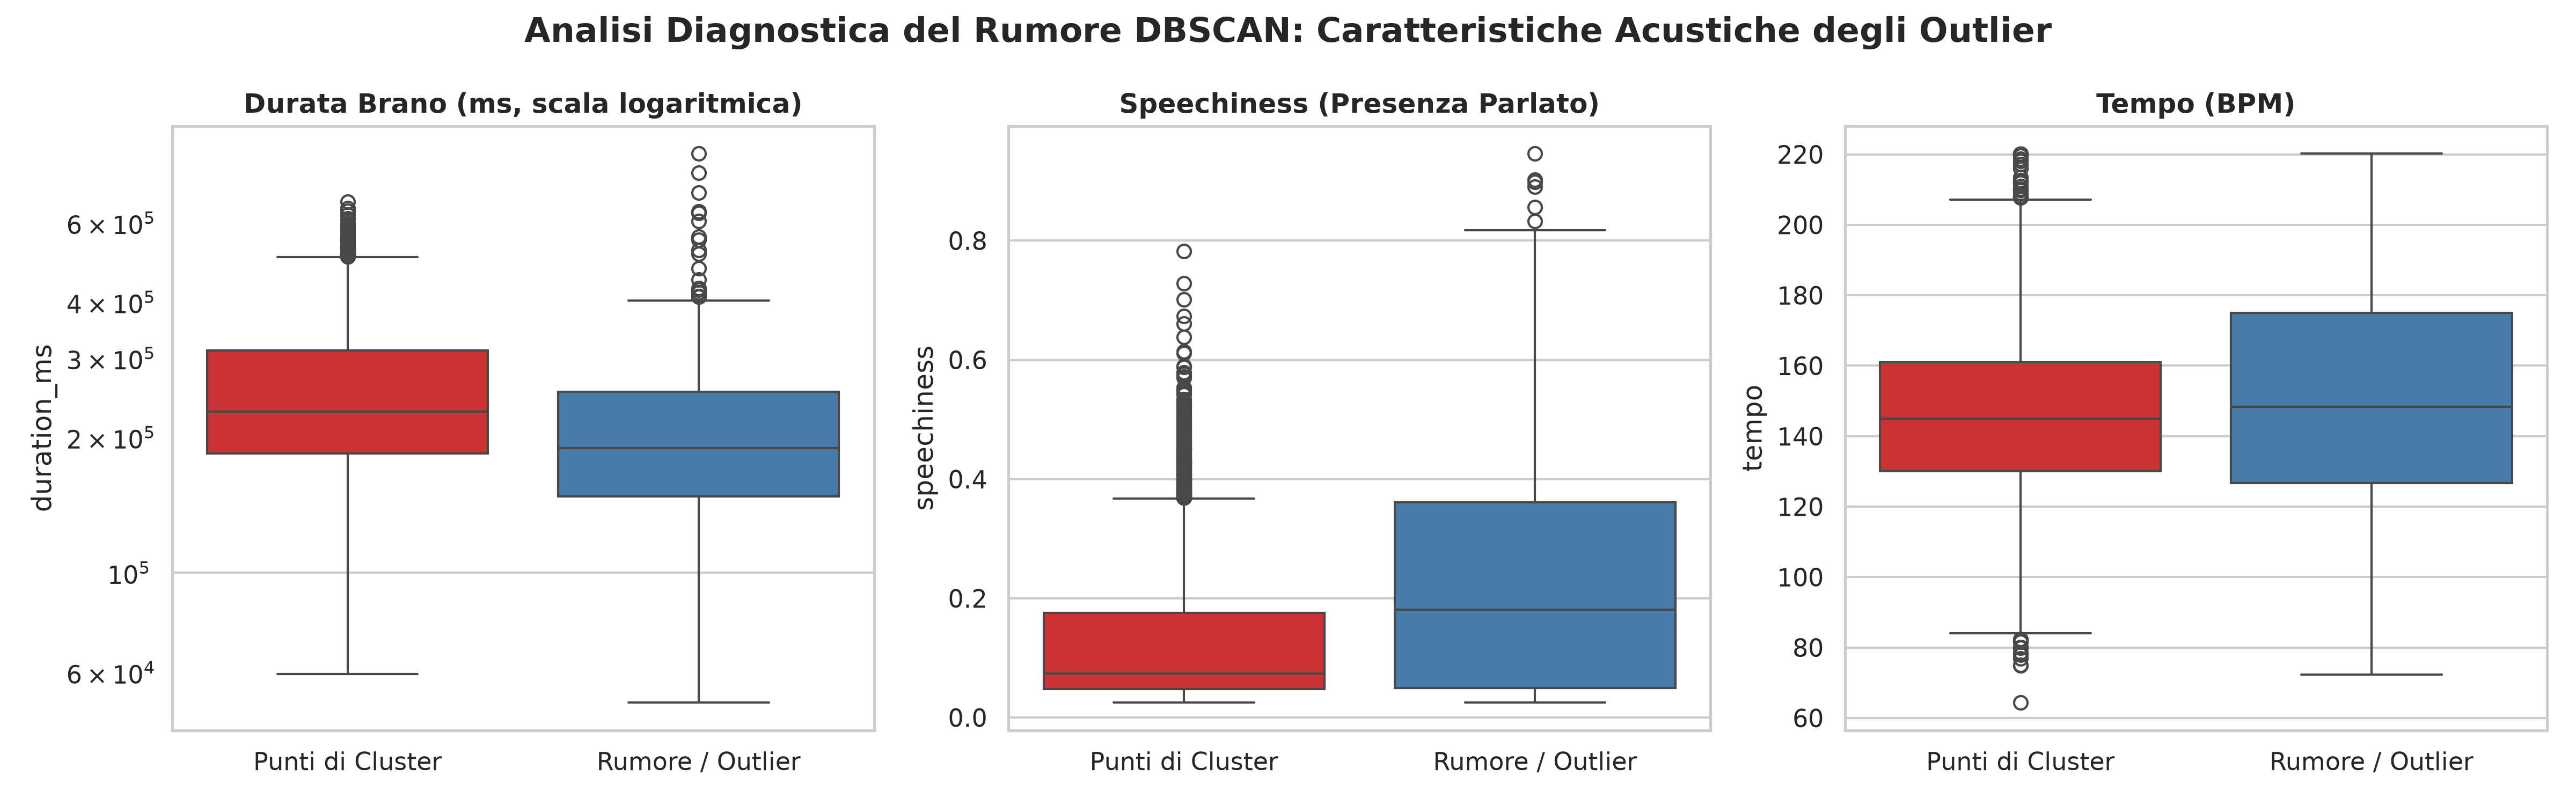
\includegraphics[width=\textwidth]{capitolo4/img/fig23_dbscan_noise_profiling.png}
    \caption{Raincloud Plot diagnostico per la separazione tra Core denso e Rumore DBSCAN: stima di densità non parametrica (Half-Violin KDE), mediana e IQR (Boxplot) e nuvola di punti reali jitterati (Rain) per le tre feature più discriminanti.}
    \label{fig:dbscan_noise}
\end{figure}

Dall'ispezione della Figura \ref{fig:dbscan_noise} emergono con evidenza le ragioni acustiche dell'isolamento metrico:
\begin{itemize}
    \item \textbf{Durata Estrema (\texttt{duration\_min}):} Mentre il Cluster Core si concentra attorno a una campana regolare centrata sullo standard radiofonico di $3,5\text{--}4$ minuti, il Rumore DBSCAN si allunga in una coda asimmetrica pronunciata che raggiunge e supera i 7--12 minuti, intercettando DJ-set continui, tracce progressive e composizioni estese non segmentate.
    \item \textbf{Speechiness Fuori Scala:} La quasi totalità del Core presenta valori di parlato minimi ($< 0,15$). La popolazione noise evidenzia invece una marcata gobba secondaria distribuita tra $0,30$ e $0,80$, catturando brani rap in metrica serrata, sketch comici, interludi parlati e podcast.
    \item \textbf{Polarizzazione Acustica (\texttt{acousticness}):} Il Core denso è pesantemente ancorato alle produzioni moderne sintetiche ed elettrificate (valori prossimi a $0$). I punti noise comprendono invece l'intera gamma delle ballate acustiche, brani per pianoforte solo e composizioni d'atmosfera con \texttt{acousticness} fino a $1,0$, la cui rarefazione nello spazio PCA le rende metricamente isolate rispetto alla folla dancefloor.
\end{itemize}

\paragraph{La Prova Empirica: il Rumore che non è Rumore.}
Nel contesto dell'ingegneria dei dati applicata all'industria discografica, emerge una conclusione fondamentale: \textbf{nella musica, il "rumore" non è mai un errore o uno scarto da cestinare, bensì una manifestazione di atipicità stilistica o di bassa densità di catalogo}. 

A comprova di ciò, sottoponendo i 462 brani noise di DBSCAN all'inferenza probabilistica del modello GMM sui 5 profili acustici, si registra un risultato sbalorditivo: la \textbf{mediana dell'affiliazione GMM più alta è pari al $92,8\%$ ($0,928$)}, e l'$85\%$ delle tracce outlier presenta un'affinità dominante superiore all'$80\%$. Ciò dimostra in modo inconfutabile che questi brani non sono affatto "rumore bianco privo di struttura", ma brani con un'identità musicale fortissima e ben definita, penalizzati unicamente dall'abitare quartieri a bassa densità demografica nello spazio metrizzato.

L'ispezione dei singoli titoli estratti dal dataset offre conferme illuminanti:
\begin{itemize}
    \item La celebre ballata pop \textit{"Unfaithful"}, espulsa da DBSCAN come noise a causa del tempo moderato e dell'intensa componente pianistica che la distanzia dalla massa ritmica da discoteca, viene riclassificata dal GMM con un'affiliazione del \textbf{$99,98\%$} alla Componente 1 (\textit{Acustico / Intimo}). Per un ascoltatore, scartarla come "rumore" sarebbe un errore madornale: si tratta invece di una traccia perfetta per una playlist da camera o relax.
    \item Il brano \textit{"Weekend (feat. Miguel)"} (catalogato come \textit{Underground Rap} con forte venatura vocale RnB), anch'esso bollato come noise da DBSCAN, ottiene un'affiliazione dell'\textbf{$87,8\%$} alla Componente 1.
    \item Tracce come \textit{"FACE"} o \textit{"Show Me Respect"} (Rap/Hiphop), isolate per via di durate non convenzionali e valori anomali di parlato, mantengono affiliazioni superiori al $53\%\text{--}60\%$ all'archetipo Urban/Ritmico (Componente 4).
\end{itemize}
DBSCAN si dimostra quindi uno straordinario strumento di \textbf{rilevamento di anomalie editoriali} (isolando skit o brani dalla struttura non convenzionale), la cui combinazione con il GMM consente di non perdere nessun brano del patrimonio musicale, assegnando a ciascun outlier la propria collocazione d'ascolto ideale.

\subsubsection{Evoluzione di DBSCAN: HDBSCAN e affiliazioni dei brani periferici}
Per verificare se la concentrazione in un unico mega-cluster dipenda dal vincolo di un raggio di vicinato $\epsilon$ rigido e costante, è stato applicato HDBSCAN (\textit{Hierarchical Density-Based Spatial Clustering of Applications with Noise}) nello stesso spazio PCA a quattro dimensioni e sul medesimo campione di $N=6.000$ brani. 

La configurazione adotta i parametri \texttt{min\_cluster\_size=30} (per evitare micro-raggruppamenti effimeri privi di valore di playlist) e \texttt{min\_samples=5} (che governa la severità della stima di densità locale tramite la distanza di raggiungibilità mutua). Esplorando gerarchicamente la persistenza della densità a scale variabili, HDBSCAN individua \textbf{10 cluster stabili} e marca come noise \textbf{4.847 brani (80,78\% del campione)}. 

Questo comportamento certifica che HDBSCAN non appiana automaticamente la periferia quando applicato su varietà continue: richiedendo una persistenza gerarchica rigorosa prima di fondere i rami del dendrogramma, l'algoritmo frammenta la megalopoli in 10 micro-comunità timbriche dense e classifica come transizione di fondo oltre l'80\% delle tracce intermedie. Nel campione, nessuno dei 462 punti noise di DBSCAN viene promosso a membro stabile di un cluster HDBSCAN; solo 22 tracce mostrano una debole affiliazione soft ($\text{max-affinity} \ge 0,10$).

\begin{figure}[H]
    \centering
    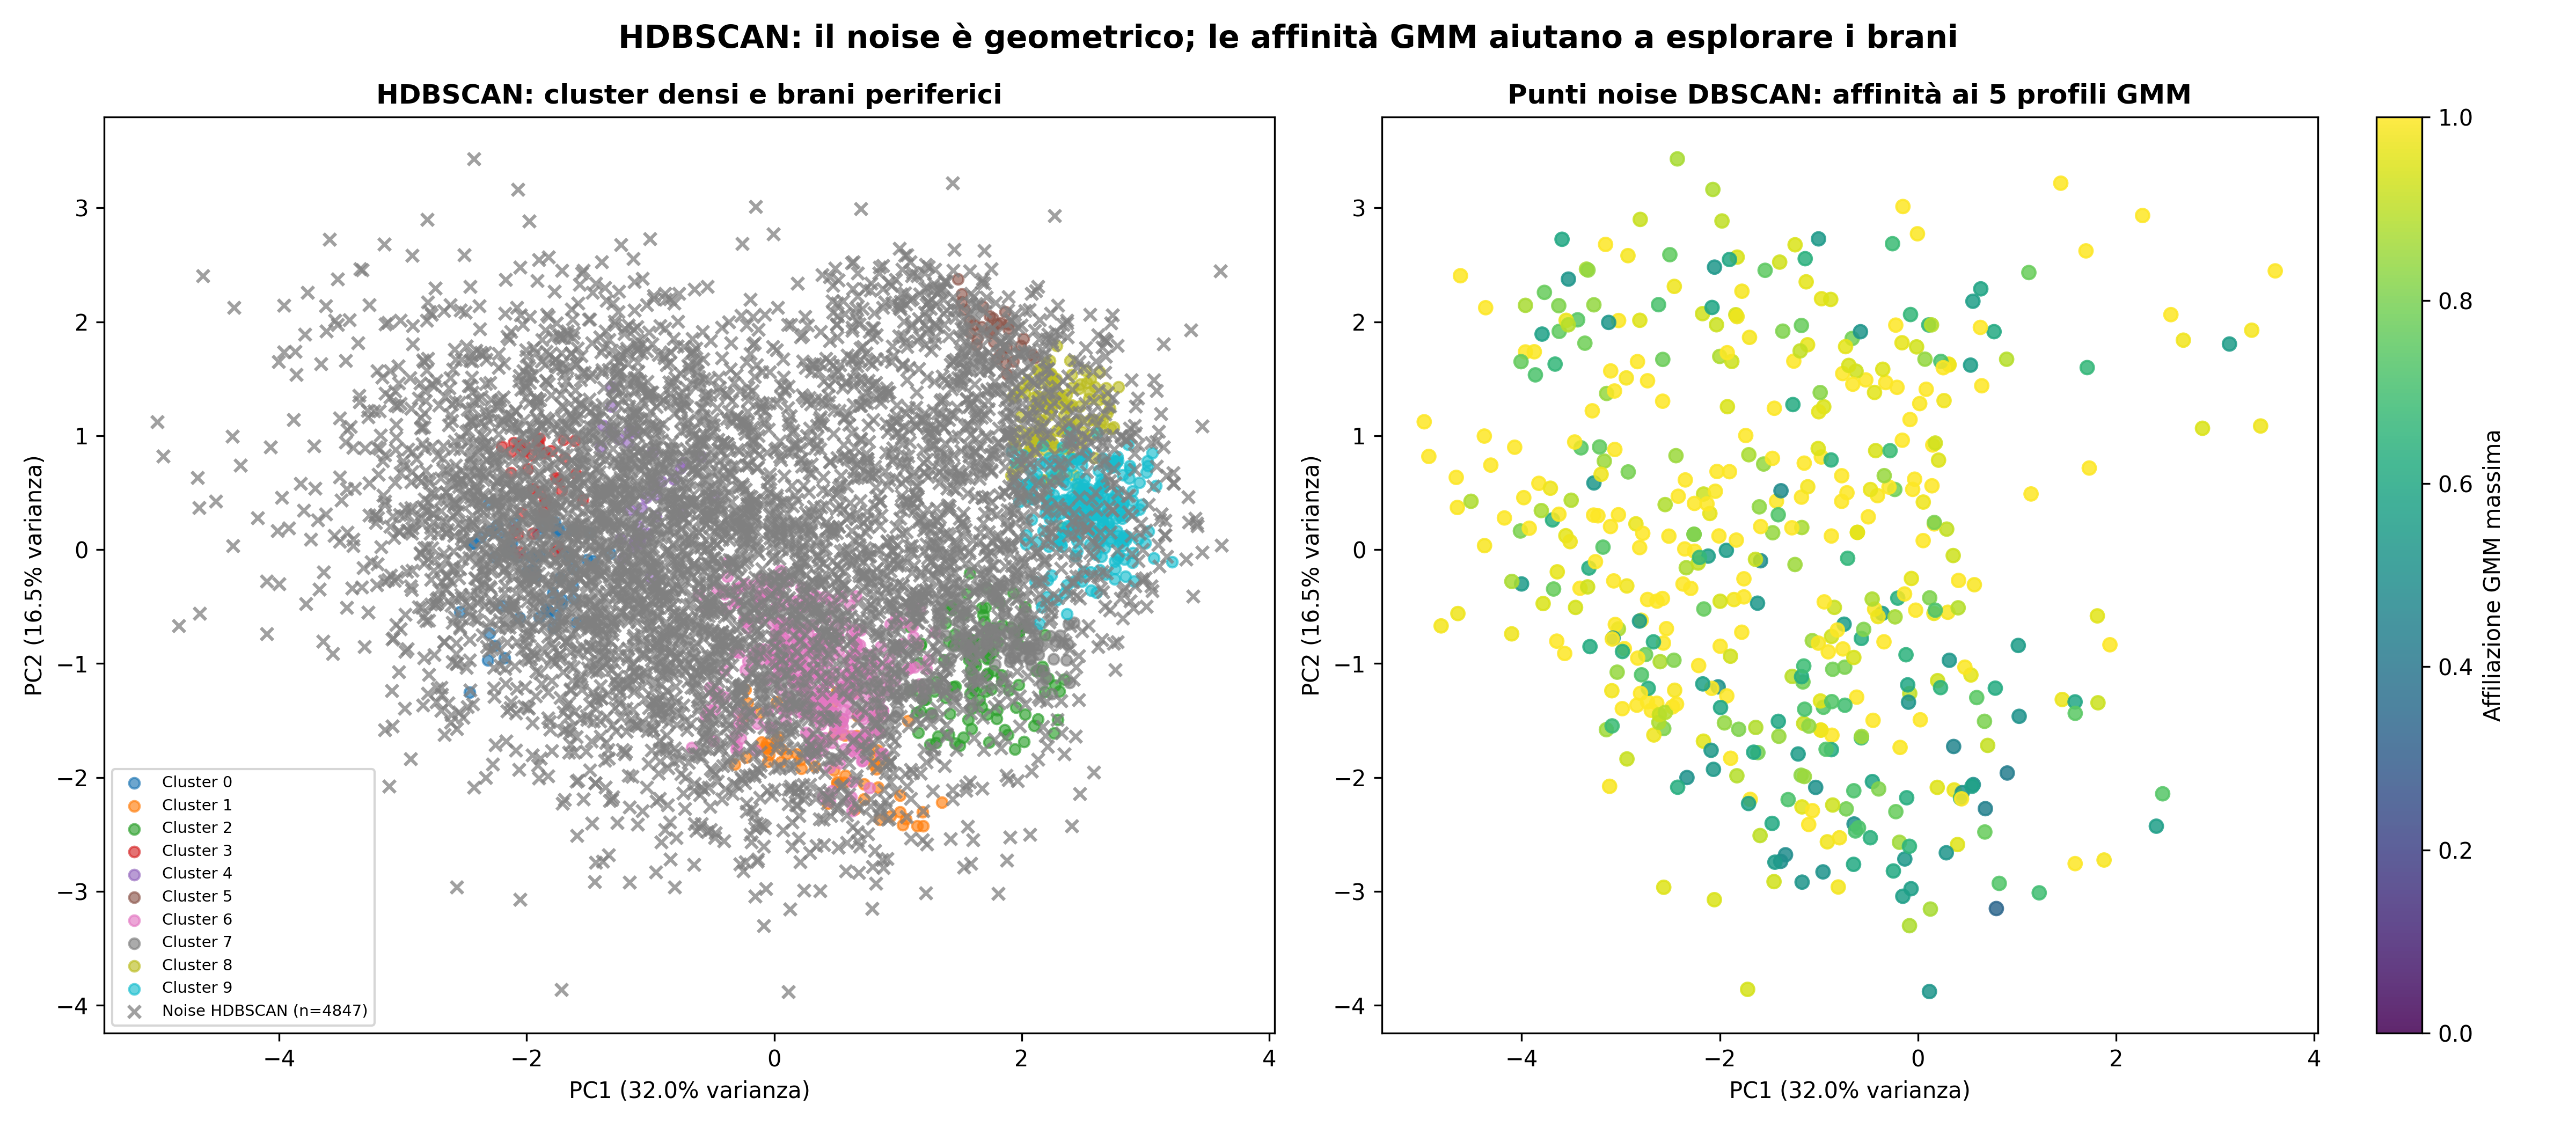
\includegraphics[width=0.96\textwidth]{capitolo4/img/fig25_hdbscan_soft_membership.png}
    \caption{Cluster HDBSCAN a densità variabile e affiliazione GMM massima dei 462 brani noise DBSCAN nella proiezione PCA 2D.}
    \label{fig:hdbscan_soft}
\end{figure}

La Figura \ref{fig:hdbscan_soft} sintetizza la convergenza dei due approcci: l'etichetta noise riflette la geometria interna di ciascun algoritmo su coordinate ipersferiche, ma non esaurisce la complessità dell'esperienza musicale. Integrando la severità topologica di DBSCAN e HDBSCAN con la flessibilità probabilistica di GMM, il catalogo può essere navigato su più livelli: partizioni per macro-mood (K-Means), ponti di transizione sfumata (GMM Soft Memberships), e filtraggio di perle rare ed eccentriche adatte a playlist di scoperta di nicchia.

\newpage
% =========================================================================
% CAPITOLO 5: BUSINESS CASE E CONCLUSIONI (SPOTIFY)
% =========================================================================
\section{Business case finale e conclusioni della Parte I}

La prima parte del presente elaborato ha sviluppato una pipeline completa di Data Science applicata all'analisi di oltre 35.000 tracce musicali estratte da Spotify, combinando pulizia dei dati, modellazione predittiva supervisionata e raggruppamento non supervisionato. L'integrazione di queste metodologie ha permesso di raggiungere conclusioni metodologiche solide e di formulare scenari applicativi di grande valore operativo per l'industria dello streaming musicale.

\subsection{Sintesi dei risultati metodologici}

\begin{itemize}
    \item \textbf{Qualità del dato ed ETL:} La corretta deduplicazione su Track ID (rimozione di 6.428 record duplicati) si è rivelata determinante per eliminare il rischio di data leakage tra set di training e test. La combinazione di SMOTE ed undersampling ha permesso di compensare efficacemente il naturale sbilanciamento delle classi senza introdurre distorsioni geometriche nelle relazioni tra attributi.
    \item \textbf{Classificazione multiclasse:} Su un problema ad elevata complessità (15 generi distinti e sole 13 feature acustiche, senza testo o metadati dell'artista), i modelli Ensemble hanno dimostrato un'eccellente capacità predittiva. Lo \textbf{Stacking Classifier} ha raggiunto un'accuratezza del \textbf{68.90\%} e un Weighted F1 di \textbf{0.6890}, supportato da una \textbf{Macro-Average ROC-AUC pari a 0.94}. L'analisi della matrice di confusione ha attestato che gli errori avvengono quasi esclusivamente tra generi contigui dal punto di vista timbrico e produttivo (Dark Trap, Underground Rap e Trap Metal).
    \item \textbf{Clustering non supervisionato nello spazio PCA:} La selezione ragionata delle 8 feature acustiche continue e la riduzione di dimensionalità mediante \textbf{PCA a 4 componenti principali (73,96\% di varianza spiegata)} hanno permesso di purificare la metrica euclidea da ridondanze e variabili categoriche. Nello spazio PCA a 4 dimensioni, il modello \textbf{K-Means con $k=5$} ha identificato 5 chiari archetipi musicali (\textit{High-Intensity Bass \& Workout, Extended Club \& Instrumental, Acoustic Chill \& Atmospheric, Groove Melodic Urban \& Pop, Fast-Flow Rap \& High-BPM}), validati da un massimo locale del coefficiente di Silhouette pari a \textbf{0,2829}. Parallelamente, l'algoritmo \textbf{DBSCAN ($\epsilon = 0,60, \texttt{min\_samples} = 5$)} ha evidenziato la natura continua del nucleo musicale principale, isolando con precisione un \textbf{7,70\% di tracce outlier (462 brani)} caratterizzate da durate estreme, parlato anomalo o combinazioni timbriche atipiche.
\end{itemize}

\subsection{Ricadute applicative e scenari di business}

I risultati conseguiti aprono la strada a tre concrete applicazioni commerciali:
\begin{enumerate}
    \item \textbf{Generazione di playlist basate sui mood (K-Means):} Le etichette di genere tradizionali risultano spesso rigide o fuorvianti: canzoni formalmente catalogate in generi diversi possono condividere lo stesso impatto emotivo e ritmico. Il partizionamento in 5 macro-mood consente alle piattaforme di streaming di generare raccomandazioni dinamiche per attività quotidiane (\textit{Workout, Focus, Chillout, Party}) basate unicamente sulle caratteristiche acustiche intrinseche della musica.
    \item \textbf{Controllo qualità e anomaly detection automatizzata (DBSCAN):} Con l'upload giornaliero di centinaia di migliaia di brani da parte di etichette indipendenti e utenti, DBSCAN costituisce un potente strumento automatico di controllo qualità, capace di intercettare file corrotti, podcast catalogati erroneamente come musica o registrazioni amatoriali difettose prima dell'indicizzazione editoriale.
    \item \textbf{Valutazione matematica di nuove uscite e demo (Classificazione Stacking):} Il modello predittivo addestrato può essere impiegato dalle case discografiche e dai team di A\&R (Artists and Repertoire) per analizzare le tracce demo appena registrate, identificandone con precisione matematica il posizionamento di genere e il pubblico di riferimento prima del lancio promozionale.
\end{enumerate}

\subsection{Sviluppi futuri}

Come sviluppi futuri per l'analisi acustica, il lavoro potrebbe essere esteso integrando tecniche multimodali: in particolare, l'analisi testuale dei testi delle canzoni (\textit{lyrics}) mediante modelli di Natural Language Processing (BERT/Transformers) e l'elaborazione degli spettrogrammi audio completi attraverso reti neurali convoluzionali (CNN). L'unione di segnali acustici, linguistici e comportamentali (storico di ascolto degli utenti) consentirà di affinare ulteriormente la precisione dei sistemi di raccomandazione musicale di nuova generazione.



% =========================================================================
% PARTE II: TIME SERIES ANALYSIS (TRANSFERMARKT)
% =========================================================================
\partseparator{PARTE II}{Analisi delle Serie Storiche sul Mercato Calcistico Europeo (Transfermarkt)}

% =========================================================================
% CAPITOLO 6: INTRODUZIONE, DATASET E PROCESSO DI ETL (TRANSFERMARKT)
% =========================================================================
\section{Analisi delle serie storiche sul mercato calcistico: introduzione e dataset}

Nel corso degli ultimi quindici anni l'industria calcistica europea ha attraversato una trasformazione economica profonda, evolvendo da settore prevalentemente sportivo a mercato finanziario globale caratterizzato da flussi di capitale miliardari, cicli stagionali regolari e forte sensibilità agli shock macroeconomici esterni. L'espansione dei diritti televisivi internazionali, l'ingresso di fondi sovrani e grandi gruppi di investimento nella proprietà dei club e l'inflazione strutturale dei costi di trasferimento hanno progressivamente ridefinito il valore patrimoniale delle rose dei principali campionati europei. In questo scenario, lo studio dell'evoluzione temporale del valore economico dei calciatori e dei volumi di spesa generati nelle sessioni di calciomercato rappresenta un banco di prova ideale per l'applicazione delle metodologie di analisi e previsione delle serie storiche.

A differenza dei mercati azionari tradizionali, dove il prezzo di un titolo viene battuto in modo continuo durante le sedute di borsa, il mercato calcistico presenta una struttura informativa composita: le valutazioni economiche dei singoli atleti vengono aggiornate periodicamente dagli analisti di mercato in finestre prestabilite durante la stagione sportiva, mentre le transazioni monetarie effettive e gli spostamenti dei giocatori tra i club si concentrano nelle due sessioni ufficiali di calciomercato (quella invernale di gennaio e quella estiva tra luglio e agosto). La seconda parte del presente elaborato si pone l'obiettivo di ricostruire, esplorare e modellare matematicamente la serie storica mensile del valore di mercato delle rose dei cinque maggiori campionati europei (Serie A, Premier League, LaLiga, Bundesliga e Ligue 1), affiancando all'analisi aggregata europea un approfondimento specifico dedicato al campionato italiano di Serie A.

Il percorso metodologico sviluppato nei capitoli successivi si articola in quattro fasi consequenziali: la progettazione di una pipeline di ingegneria dei dati capace di trasformare le tabelle relazionali grezze in una serie storica mensile regolare e priva di discontinuità artificiali; l'analisi esplorativa dei dati e lo studio quantitativo dei grandi shock storici che hanno colpito il settore (dall'esplosione inflattiva del 2017 legata al trasferimento record di Neymar fino alla contrazione pandemica del 2020 e al successivo rimbalzo post-pandemico); la decomposizione stagionale e la verifica formale delle proprietà di stazionarietà e autocorrelazione temporale; infine, l'addestramento e il confronto critico di modelli previsionali di complessità crescente, dai modelli autoregressivi classici fino ai modelli stagionali con variabili esogene (dove il volume di spesa e il numero di trasferimenti del calciomercato vengono impiegati come predittori esterni della dinamica del valore delle rose).

\subsection{Struttura del dataset relazionale di Transfermarkt}

La base informativa utilizzata per lo studio proviene dal repository pubblico \textit{Football Data from Transfermarkt} distribuito sulla piattaforma Kaggle. A differenza di un dataset nativo di serie storiche, la fonte originale è organizzata come un database relazionale composto da dodici tabelle distinte in formato \texttt{.csv}, che registrano l'anagrafica dei campionati, dei club e dei giocatori insieme allo storico granulare delle partite disputate, delle presenze individuali, dei trasferimenti ufficiali e delle valutazioni di mercato.

Per la costruzione della serie storica del valore patrimoniale delle rose e dei flussi di calciomercato, l'attenzione si è concentrata sulle cinque tabelle fondamentali riassunte nella Tabella \ref{tab:tabelle_transfermarkt}. La tabella centrale è costituita dal file \texttt{player\_valuations.csv}, che raccoglie 656.301 osservazioni storiche relative alle stime di valore di mercato espresse in euro (\texttt{market\_value\_in\_eur}) attribuite a ciascun calciatore identificato tramite la chiave primaria \texttt{player\_id} in una determinata data (\texttt{date}). A questa si affianca il file \texttt{transfers.csv}, contenente 175.165 record di trasferimento che documentano per ogni operazione la data esatta (\texttt{transfer\_date}), il club di provenienza (\texttt{from\_club\_id}), il club di destinazione (\texttt{to\_club\_id}), il corrispettivo economico pagato per il cartellino (\texttt{transfer\_fee}) e la valutazione del giocatore al momento del passaggio.

\begin{table}[H]
\centering
\caption{Riepilogo delle tabelle relazionali del dataset di Transfermarkt utilizzate nella pipeline.}
\label{tab:tabelle_transfermarkt}
\begin{tabular}{llrl}
\toprule
\textbf{File sorgente} & \textbf{Chiavi principali} & \textbf{Record grezzi} & \textbf{Ruolo nella ricostruzione temporale} \\
\midrule
\texttt{player\_valuations.csv} & \texttt{player\_id}, \texttt{date} & 656.301 & Storico delle valutazioni di mercato in euro \\
\texttt{transfers.csv} & \texttt{player\_id}, \texttt{transfer\_date} & 175.165 & Spostamenti tra club e volume spese (\texttt{transfer\_fee}) \\
\texttt{appearances.csv} & \texttt{player\_id}, \texttt{date} & 1.894.350 & Presenze effettive e verifica del club storico (\texttt{player\_club\_id}) \\
\texttt{clubs.csv} & \texttt{club\_id} & 796 & Anagrafica dei club e lega di appartenenza \\
\texttt{competitions.csv} & \texttt{competition\_id} & 65 & Codifica dei cinque maggiori campionati europei \\
\bottomrule
\end{tabular}
\end{table}

L'integrazione con la tabella \texttt{appearances.csv}, che conta 1.894.350 registrazioni di presenze individuali in gara, e con i dizionari anagrafici \texttt{clubs.csv} e \texttt{competitions.csv} consente di associare ogni società calcistica alla rispettiva lega nazionale mediante il codice identificativo \texttt{domestic\_competition\_id}. In particolare, il perimetro dello studio seleziona i cinque massimi campionati europei: la Serie A italiana (\texttt{IT1}), la Premier League inglese (\texttt{GB1}), LaLiga spagnola (\texttt{ES1}), la Bundesliga tedesca (\texttt{L1}) e la Ligue 1 francese (\texttt{FR1}).

\newpage
\subsection{Processo di estrazione, trasformazione e caricamento per la serie storica}

La trasformazione dei record puntuali di Transfermarkt in una serie storica rigorosa richiede di risolvere due criticità strutturali intrinseche ai dati grezzi, che se trascurate comprometterebbero la regolarità degli intervalli temporali e la veridicità economica dei valori aggregati. L'intera procedura descritta di seguito è stata implementata in modo riproducibile all'interno dello script \texttt{01\_etl\_transfermarkt.py}.

La prima criticità riguarda la frequenza di campionamento e la complementarità tra listini di valutazione e sessioni di mercato. Nel file \texttt{player\_valuations.csv}, le revisioni dei prezzi non avvengono simultaneamente in tutti i mesi dell'anno per l'intero organico dei campionati, ma si concentrano prevalentemente in quattro finestre stagionali (marzo, fine maggio e giugno, ottobre e dicembre). Al contrario, nei mesi di gennaio, febbraio, luglio e agosto il numero di aggiornamenti di listino è ridotto poiché gli analisti attendono la chiusura delle trattative ufficiali; tuttavia, proprio in questi mesi il file \texttt{transfers.csv} registra migliaia di compravendite che modificano profondamente la composizione e il valore patrimoniale delle rose. 

Questa dinamica complementare è documentata nella Figura \ref{fig:etl_complementarita}: nel pannello di sinistra si osserva come i mesi con minori revisioni di prezzo in \texttt{player\_valuations.csv} coincidano esattamente con i picchi di attività di \texttt{transfers.csv} (luglio, agosto e gennaio), mentre il pannello di destra evidenzia come il volume medio di spesa mensile superi i 2.300 milioni di euro nel mese di luglio, i 1.280 milioni in agosto e i 550 milioni a gennaio.

\begin{figure}[H]
    \centering
    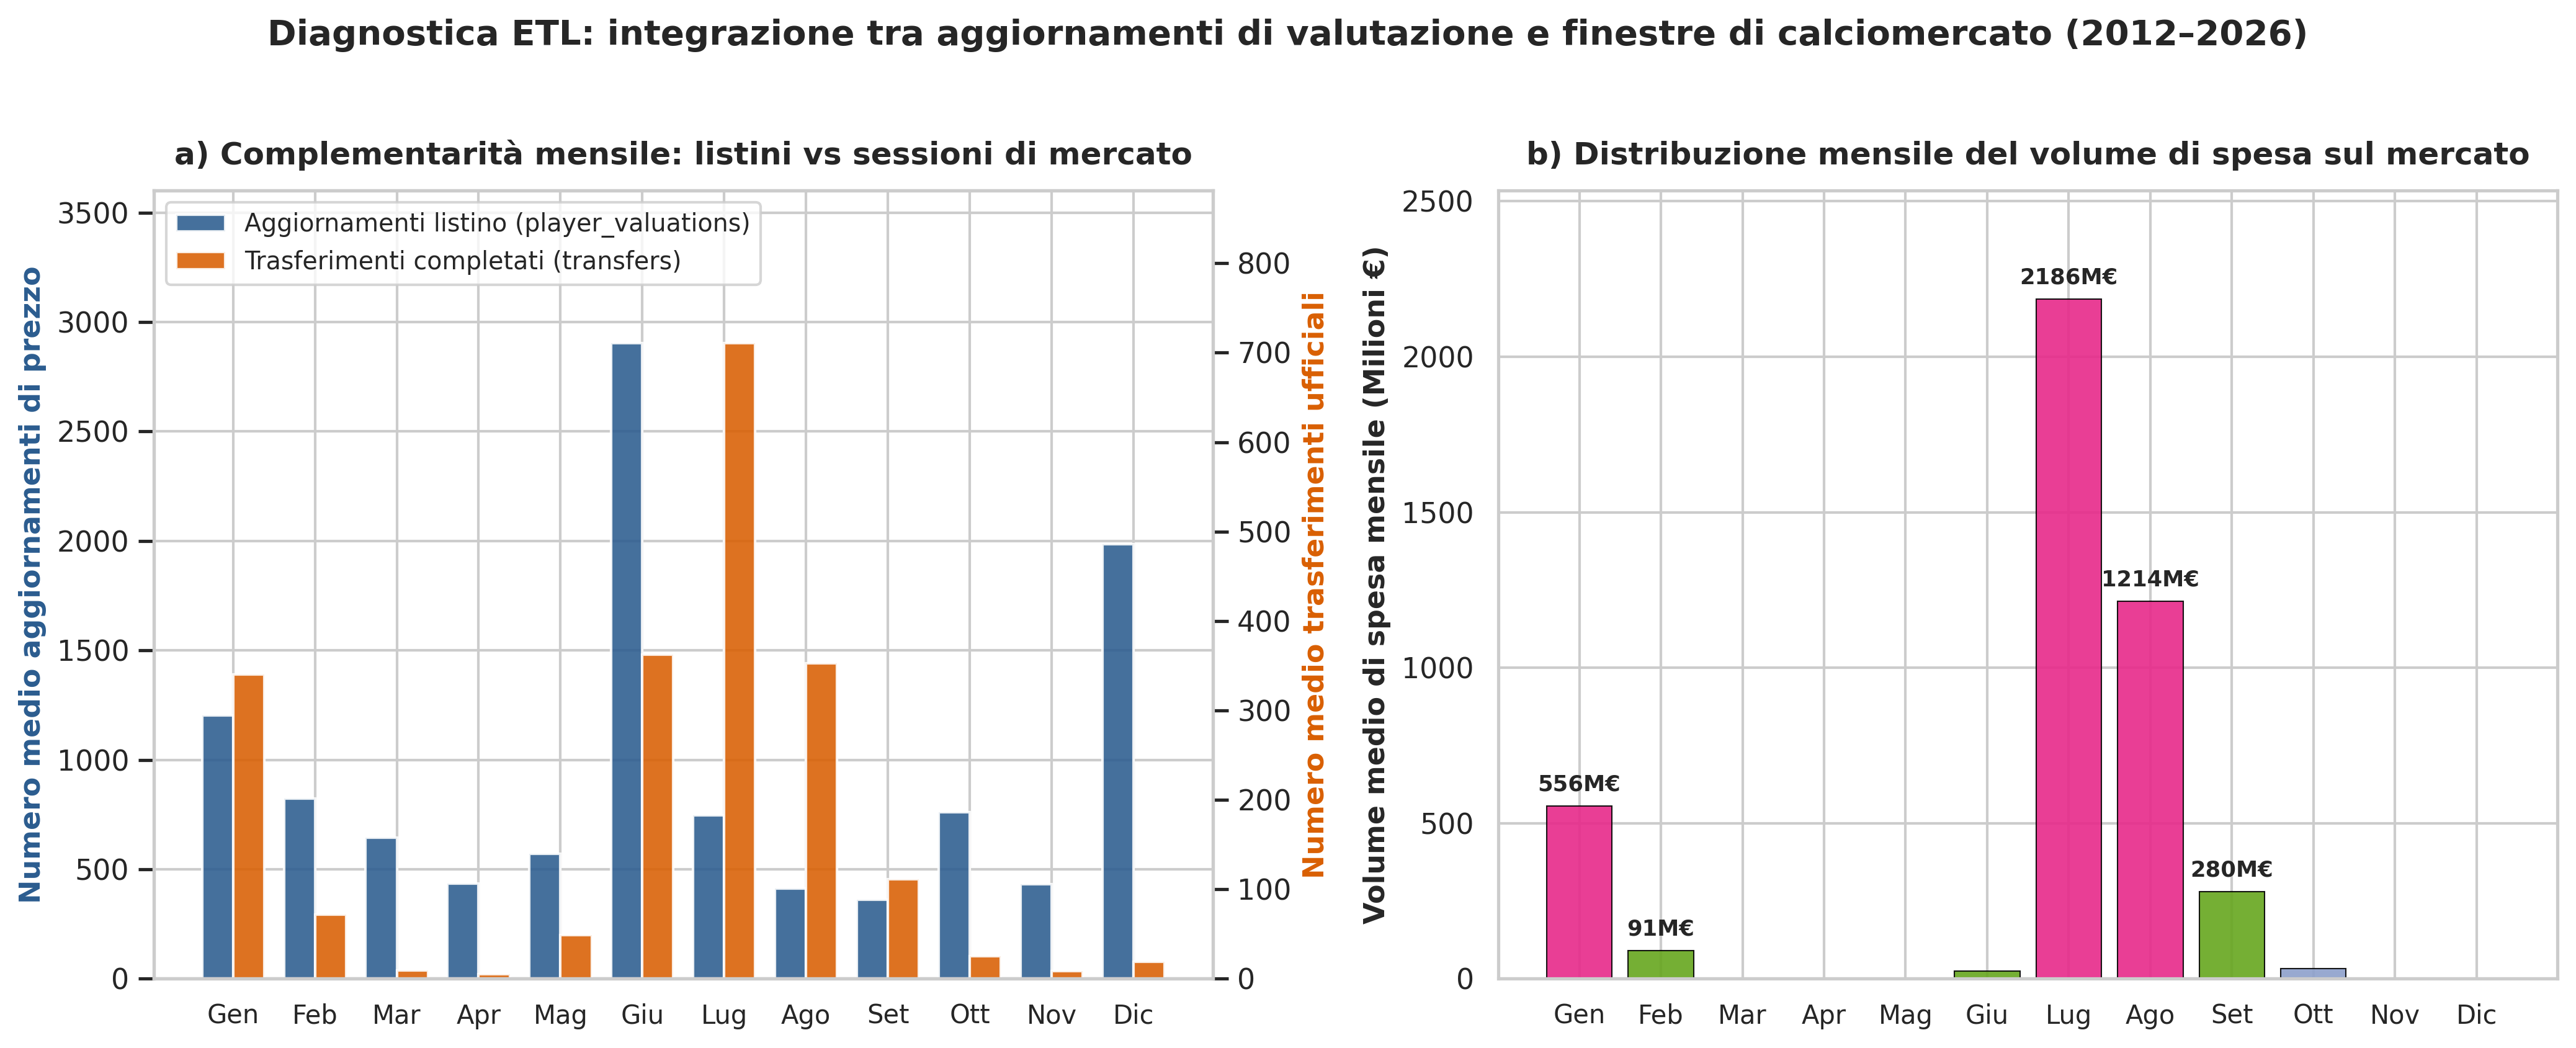
\includegraphics[width=0.98\textwidth]{capitolo6/img/fig01_etl_complementarita_fonti.png}
    \caption{Complementarità stagionale tra la frequenza mensile degli aggiornamenti di valutazione e il volume delle operazioni di calciomercato nei cinque maggiori campionati europei.}
    \label{fig:etl_complementarita}
\end{figure}

Se si aggregassero ingenuamente le sole righe di \texttt{player\_valuations.csv} mese per mese senza mantenere lo stato patrimoniale dei giocatori in attività, la serie risultante rifletterebbe il numero di aggiornamenti redazionali anziché il reale valore delle rose. D'altra parte, se si applicasse una semplice propagazione in avanti delle valutazioni senza tenere conto dei trasferimenti di mercato, la serie presenterebbe dei tratti quasi costanti nei mesi in cui i listini sono fermi.

La seconda criticità riguarda la distorsione retrospettiva legata all'appartenenza dei giocatori ai club. All'interno della tabella \texttt{player\_valuations.csv}, gli attributi \texttt{current\_club\_id} e \texttt{player\_club\_domestic\_competition\_id} non sono variabili storiche indicizzate nel tempo, bensì campi statici che riportano unicamente l'ultima squadra in cui il calciatore milita al momento dell'estrazione del dataset (nel 2026). Di conseguenza, un'aggregazione basata direttamente su tale colonna attribuirebbe l'intera storia passata di un giocatore al suo campionato del 2026: a titolo esemplificativo, atleti protagonisti in Serie A tra il 2018 e il 2021 ma successivamente trasferitisi all'estero (o ritiratisi) non verrebbero conteggiati nel valore storico del campionato italiano, generando una grave sottostima retrospettiva.

Per superare entrambe le problematiche, l'algoritmo di ricostruzione storica implementato nel Listato \ref{lst:etl_ricostruzione} costruisce una griglia temporale mensile regolare (con fase di inizializzazione a partire da gennaio 2009 e finestra di analisi da giugno 2011 a maggio 2026, per un totale di 180 mesi consecutivi pari a quindici cicli annuali completi) ed esegue l'allineamento congiunto dello stato di prezzo e dello stato di appartenenza al club per ciascun giocatore.

\begin{lstlisting}[language=Python, caption={Ricostruzione storica mensile del valore di mercato e del club di appartenenza nello script \texttt{01\_etl\_transfermarkt.py}.}, label={lst:etl_ricostruzione}]
# 1. Griglia mensile regolare e propagazione controllata dell'ultima valutazione valida
grid_months = pd.period_range("2009-01", "2026-05", freq="M")
target_months = pd.period_range("2011-06", "2026-05", freq="M")  # 180 mesi (15 anni)

val_m = vals_sub.groupby(["player_id", "year_month"])["market_value_in_eur"].last().unstack(level=0)
val_ff = val_m.reindex(grid_months).ffill(limit=18)

# 2. Ricostruzione del club storico mese per mese da presenze (appearances) e trasferimenti (transfers)
app_club_m = app_sub.groupby(["player_id", "year_month"])["player_club_id"].last()
tr_club_m = tr_sub.groupby(["player_id", "year_month"])["to_club_id"].last()

club_events = pd.concat([app_club_m, tr_club_m]).groupby(level=[0, 1]).last().unstack(level=0)
club_events = club_events.reindex(index=grid_months, columns=val_ff.columns)
club_hist = club_events.ffill().bfill().fillna(val_club_m)

# 3. Mappatura dal club storico alla rispettiva lega nazionale (IT1, GB1, ES1, L1, FR1)
comp_hist = club_hist.apply(lambda col: col.map(club_to_comp)).fillna("OTHER")
\end{lstlisting}

Come illustrato nel Listato \ref{lst:etl_ricostruzione}, per ogni calciatore e per ciascun mese della griglia temporale viene mantenuta l'ultima valutazione di mercato valida mediante operazione di \textit{forward-fill} limitata a un orizzonte massimo di diciotto mesi, così da garantire la continuità della quotazione per tutti i giocatori in attività ed escludere automaticamente dal computo gli atleti ritirati o inattivi. Contemporaneamente, la matricola del club in cui il giocatore milita in quel preciso mese viene determinata incrociando cronologicamente le presenze effettive in campo tratte da \texttt{appearances.csv} (\texttt{player\_club\_id}) e i cambi di casacca registrati in \texttt{transfers.csv} (\texttt{to\_club\_id}), mappando poi il club storico alla rispettiva competizione nazionale tramite il dizionario estratto da \texttt{clubs.csv}.

L'efficacia di questa ricostruzione ingegneristica è dimostrata visivamente nella Figura \ref{fig:etl_confronto}. Nel pannello superiore viene messo a confronto il valore storico della Serie A ottenuto tramite la nostra ricostruzione dinamica (linea continua verde) con quello prodotto da un'aggregazione statica basata sul solo club del 2026 (linea tratteggiata arancione): quest'ultima sottostima sistematicamente il patrimonio della Serie A lungo tutto il decennio 2014--2022, arrivando a perdere quasi un miliardo di euro di valore reale nel biennio 2019--2020. Al contrario, la serie ricostruita cattura fedelmente sia le acquisizioni internazionali durante le finestre estive e invernali, sia le revisioni periodiche dei cartellini durante il campionato. Nel pannello inferiore della Figura \ref{fig:etl_confronto} è riportata la serie storica principale post-ETL del valore aggregato dei cinque maggiori campionati europei, che evolve in modo continuo da 11,12 miliardi di euro nel giugno 2011 fino al massimo storico di 34,44 miliardi di euro nel maggio 2026.

\begin{figure}[H]
    \centering
    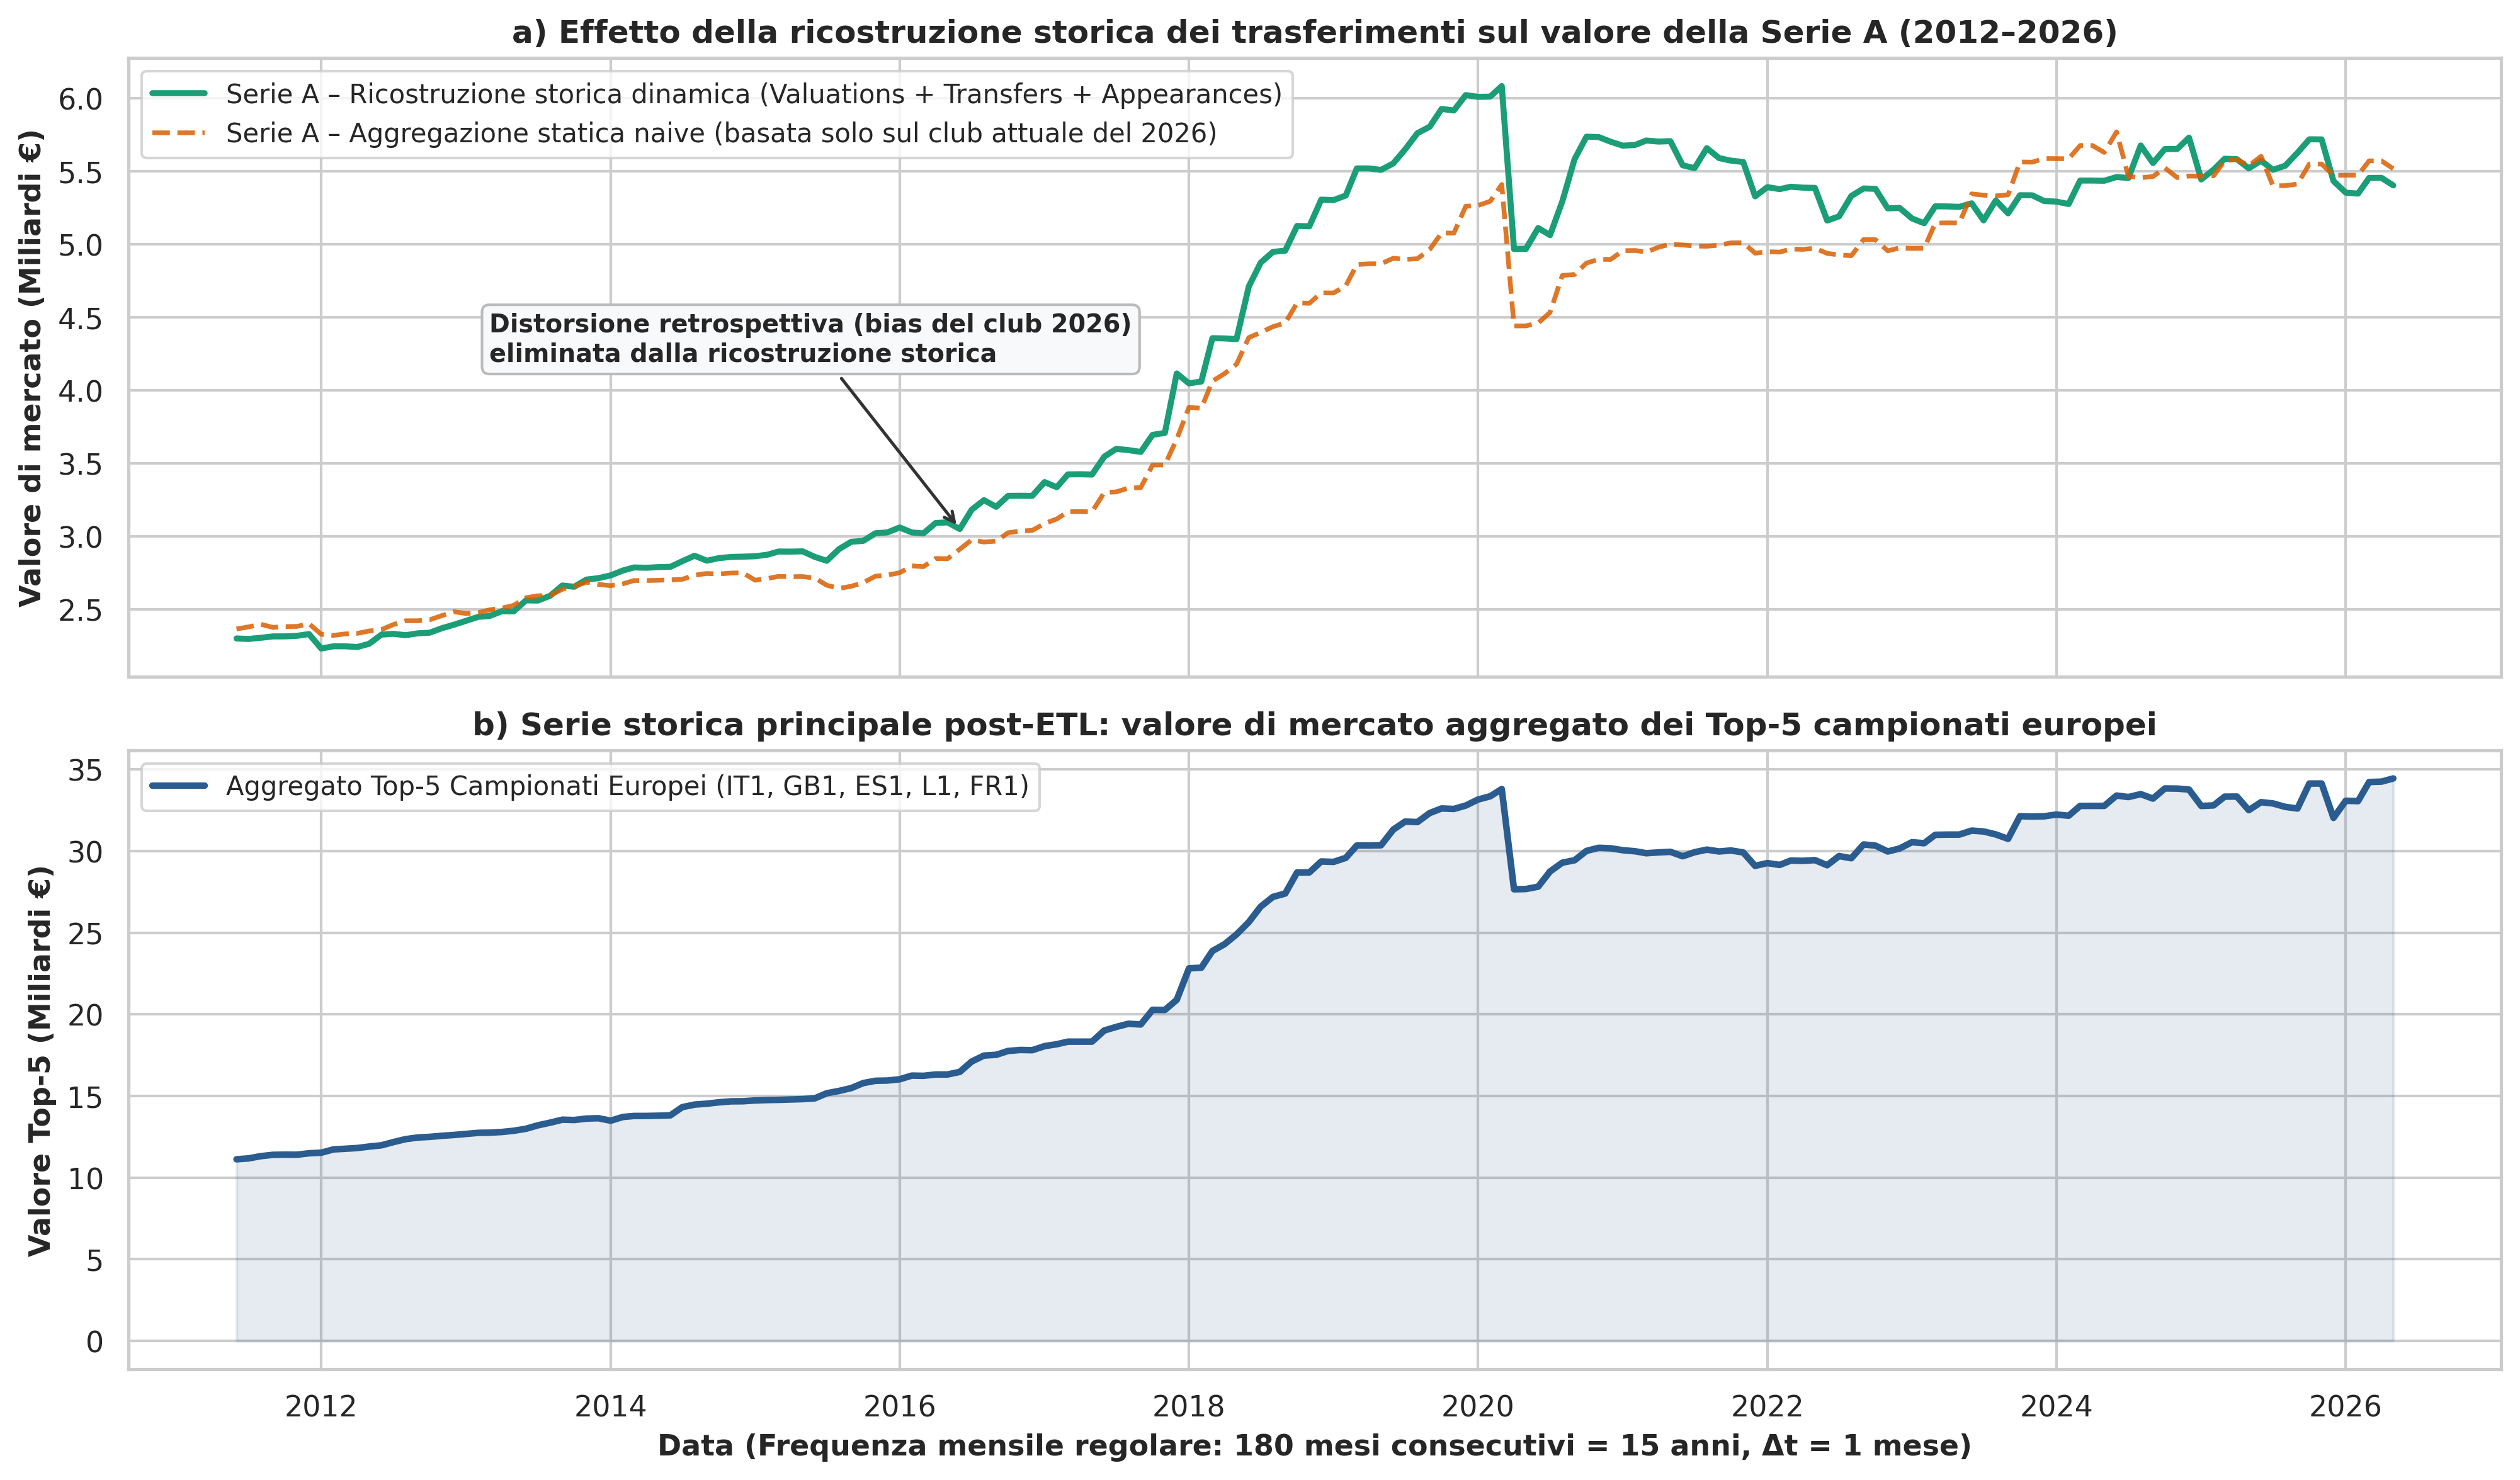
\includegraphics[width=0.98\textwidth]{capitolo6/img/fig02_etl_ricostruzione_storica_confronto.png}
    \caption{Confronto tra aggregazione statica e ricostruzione storica dinamica per la Serie A e andamento complessivo della serie storica principale post-ETL sui 180 mesi di osservazione.}
    \label{fig:etl_confronto}
\end{figure}

La scelta di fissare l'orizzonte temporale definitivo tra giugno 2011 (\texttt{2011-06}) e maggio 2026 (\texttt{2026-05}) risponde a due criteri metodologici rigorosi: da un lato consente di escludere il mese di giugno 2026, parzialmente incompleto nell'estrazione originale e affetto dalla pre-registrazione automatica delle scadenze contrattuali di fine stagione; dall'altro fornisce esattamente 180 osservazioni mensili consecutive, corrispondenti a quindici cicli annuali completi di dodici mesi ($s = 12$). Tale cardinalità permette una suddivisione temporale ottimale per la successiva fase di modellazione predittiva, destinando i primi dodici anni completi (144 mesi, pari all'80\% del campione) al set di addestramento e gli ultimi tre anni completi (36 mesi, pari al 20\%) al set di test.

\begin{table}[H]
\centering
\caption{Struttura delle variabili principali contenute nel dataset mensile elaborato \texttt{market\_monthly.csv}.}
\label{tab:schema_market_monthly}
\begin{tabular}{lll}
\toprule
\textbf{Variabile} & \textbf{Unita / Tipo} & \textbf{Descrizione} \\
\midrule
\texttt{year\_month}, \texttt{date} & Data mensile & Indice temporale regolare ($\Delta t = 1$ mese, 180 osservazioni) \\
\texttt{top5\_market\_value\_bn} & Float (Mld EUR) & Valore di mercato aggregato delle rose dei Top-5 campionati \\
\texttt{serie\_a\_market\_value\_bn} & Float (Mld EUR) & Valore di mercato aggregato delle rose della Serie A (\texttt{IT1}) \\
\texttt{premier\_league\_market\_value\_bn} & Float (Mld EUR) & Valore di mercato aggregato della Premier League (\texttt{GB1}) \\
\texttt{laliga\_market\_value\_bn} & Float (Mld EUR) & Valore di mercato aggregato de LaLiga (\texttt{ES1}) \\
\texttt{bundesliga\_market\_value\_bn} & Float (Mld EUR) & Valore di mercato aggregato della Bundesliga (\texttt{L1}) \\
\texttt{ligue1\_market\_value\_bn} & Float (Mld EUR) & Valore di mercato aggregato della Ligue 1 (\texttt{FR1}) \\
\texttt{mean\_player\_value\_m} & Float (Mln EUR) & Valore di mercato medio per calciatore attivo nei Top-5 \\
\texttt{transfer\_spend\_top5\_m} & Float (Mln EUR) & Volume mensile di spesa per trasferimenti onerosi nei Top-5 \\
\texttt{transfer\_spend\_serie\_a\_m} & Float (Mln EUR) & Volume mensile di spesa per trasferimenti in Serie A \\
\texttt{n\_transfers\_top5} & Intero & Numero totale di trasferimenti completati nel mese \\
\texttt{overpay\_ratio} & Float & Rapporto mediano tra prezzo pagato e valore di mercato \\
\texttt{pct\_change\_top5} & Float (\%) & Variazione percentuale mensile del valore aggregato Top-5 \\
\texttt{shock\_neymar\_post2017} & Binaria [0/1] & Indicatore del regime post-agosto 2017 (shock inflattivo) \\
\texttt{shock\_covid\_2020} & Binaria [0/1] & Indicatore della finestra pandemica e del taglio di aprile 2020 \\
\bottomrule
\end{tabular}
\end{table}

I controlli di integrità eseguiti al termine della pipeline ed esportati nel file di certificazione \texttt{etl\_summary.json} attestano la totale assenza di valori nulli o mesi mancanti (\texttt{missing\_months = 0} su 180 osservazioni) e confermano che la serie principale \texttt{top5\_market\_value\_bn} presenta variazioni non nulle in 179 transizioni mensili consecutive su 179 (\texttt{zero\_change\_months = 0}), soddisfacendo pienamente sia il requisito di equispaziatura temporale sia quello di variabilità dinamica continua. Nella Tabella \ref{tab:schema_market_monthly} vengono infine riassunte le principali variabili salvate all'interno del dataset definitivo \texttt{market\_monthly.csv}, che costituisce la base di partenza per l'analisi esplorativa e la modellazione dei capitoli seguenti.


\newpage
% =========================================================================
% CAPITOLO 7: ANALISI ESPLORATIVA DEI DATI E DINAMICA DEGLI SHOCK STORICI
% =========================================================================
\section{Analisi esplorativa della serie storica e dinamica degli shock di mercato}

Una volta certificata la regolarità temporale e la coerenza retrospettiva del dataset mensile post-ETL \texttt{market\_monthly.csv}, il secondo passo metodologico consiste nell'analisi esplorativa della serie storica (\textit{Exploratory Data Analysis}, EDA) lungo l'intero orizzonte di 180 osservazioni mensili compreso tra giugno 2011 (\texttt{2011-06}) e maggio 2026 (\texttt{2026-05}). L'obiettivo di questa fase, implementata all'interno dello script \texttt{02\_eda\_e\_shock.py}, è triplice: caratterizzare l'evoluzione di lungo periodo e i rapporti di forza tra i cinque maggiori campionati europei, isolare e quantificare l'impatto dei tre grandi shock strutturali che hanno colpito il settore calcistico nell'ultimo quindicennio e indagare la relazione dinamica tra la serie delle valutazioni patrimoniali delle rose e il volume delle spese effettuate durante le sessioni di calciomercato.

\subsection{Evoluzione comparata dei cinque campionati europei e divario strutturale}

L'osservazione congiunta delle cinque massime divisioni europee mette in luce come la crescita complessiva del valore aggregato delle rose, passato da 11,12 miliardi di euro nel giugno 2011 a 34,44 miliardi di euro nel maggio 2026 (+209,7\%), non si sia distribuita in modo uniforme tra le diverse leghe nazionali, ma abbia generato una progressiva polarizzazione finanziaria guidata dalla Premier League inglese. 

Nella Figura \ref{fig:eda_valore_campionati} viene illustrata l'evoluzione temporale del valore di mercato assoluto di ciascun campionato, evidenziando le date cardine dei tre grandi shock macroeconomici.

\begin{figure}[H]
    \centering
    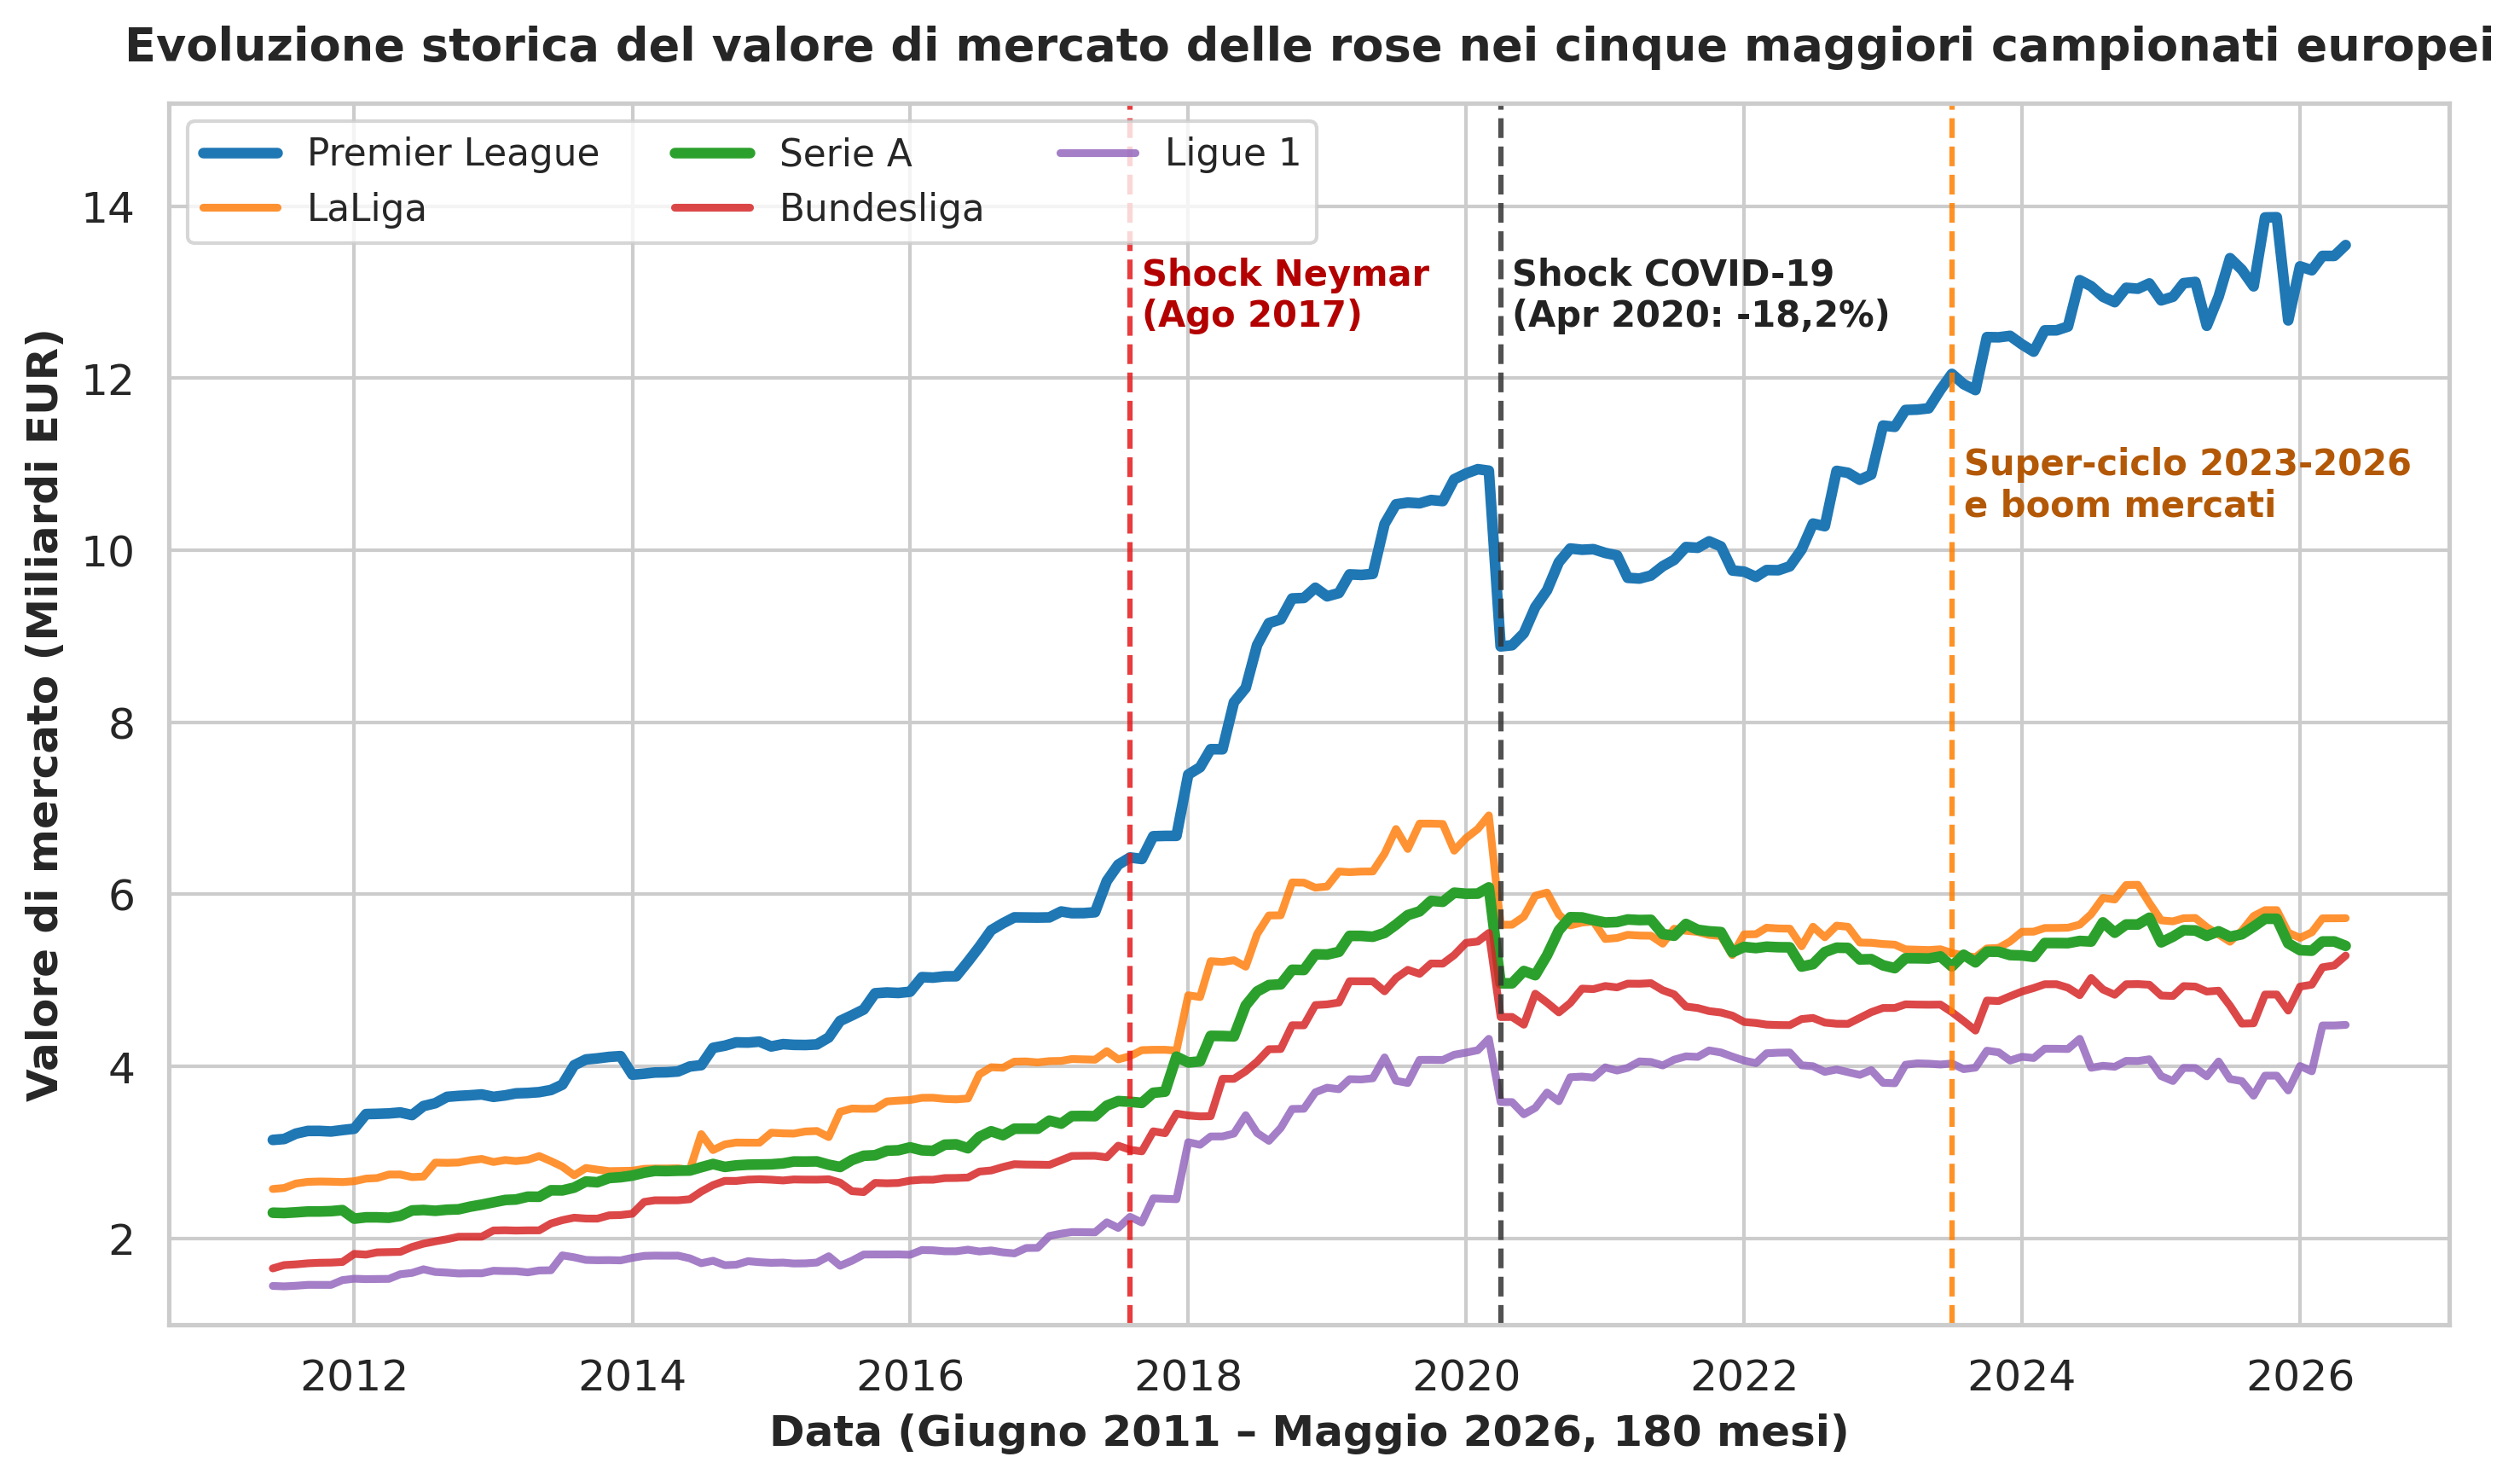
\includegraphics[width=0.95\textwidth]{capitolo7/img/fig03_eda_valore_campionati.png}
    \caption{Evoluzione storica del valore di mercato delle rose nei cinque maggiori campionati europei tra giugno 2011 e maggio 2026.}
    \label{fig:eda_valore_campionati}
\end{figure}

Come emerge con chiarezza dalla Figura \ref{fig:eda_valore_campionati} e dal confronto quantitativo riportato nella Tabella \ref{tab:confronto_leghe_shock}, all'inizio della finestra di analisi (\texttt{2011-06}) il mercato calcistico europeo presentava un assetto relativamente bilanciato: la Premier League deteneva un valore complessivo di 3,15 miliardi di euro, seguita a breve distanza da LaLiga spagnola con 2,58 miliardi e dalla Serie A italiana con 2,30 miliardi, mentre la Bundesliga tedesca (1,65 miliardi) e la Ligue 1 francese (1,45 miliardi) completavano il perimetro dei cinque tornei.

\begin{table}[H]
\centering
\caption{Confronto del valore di mercato delle rose (in miliardi di euro) e delle variazioni percentuali nei cinque campionati europei attraverso le date chiave della serie storica.}
\label{tab:confronto_leghe_shock}
\begin{tabularx}{\textwidth}{lXXXXXXX}
\toprule
\textbf{Campionato} & \textbf{Giu 11} & \textbf{Lug 17} & \textbf{Mar 20} & \textbf{Apr 20} & \textbf{Mag 26} & \textbf{$\Delta\%$ COVID} & \textbf{$\Delta\%$ 15 anni} \\
\midrule
Premier League (\texttt{GB1}) & 3,15 & 6,35 & 10,92 & 8,88 & 13,55 & $-18,70\%$ & $+330,6\%$ \\
LaLiga (\texttt{ES1}) & 2,58 & 4,08 & 6,92 & 5,65 & 5,72 & $-18,36\%$ & $+122,2\%$ \\
Serie A (\texttt{IT1}) & 2,30 & 3,60 & 6,08 & 4,97 & 5,40 & $-18,34\%$ & $+134,9\%$ \\
Bundesliga (\texttt{L1}) & 1,65 & 3,08 & 5,55 & 4,57 & 5,29 & $-17,60\%$ & $+220,0\%$ \\
Ligue 1 (\texttt{FR1}) & 1,45 & 2,12 & 4,32 & 3,59 & 4,48 & $-17,01\%$ & $+209,4\%$ \\
\midrule
\textbf{Totale Top-5} & \textbf{11,12} & \textbf{19,23} & \textbf{33,79} & \textbf{27,65} & \textbf{34,44} & \textbf{$-18,17\%$} & \textbf{$+209,7\%$} \\
\bottomrule
\end{tabularx}
\end{table}

La progressiva trasformazione dei rapporti di forza è resa evidente dalla dinamica delle quote percentuali sul totale continentale (\textit{Market Share \%}), rappresentata mediante area cumulativa nella Figura \ref{fig:eda_quote_mercato}.

\begin{figure}[H]
    \centering
    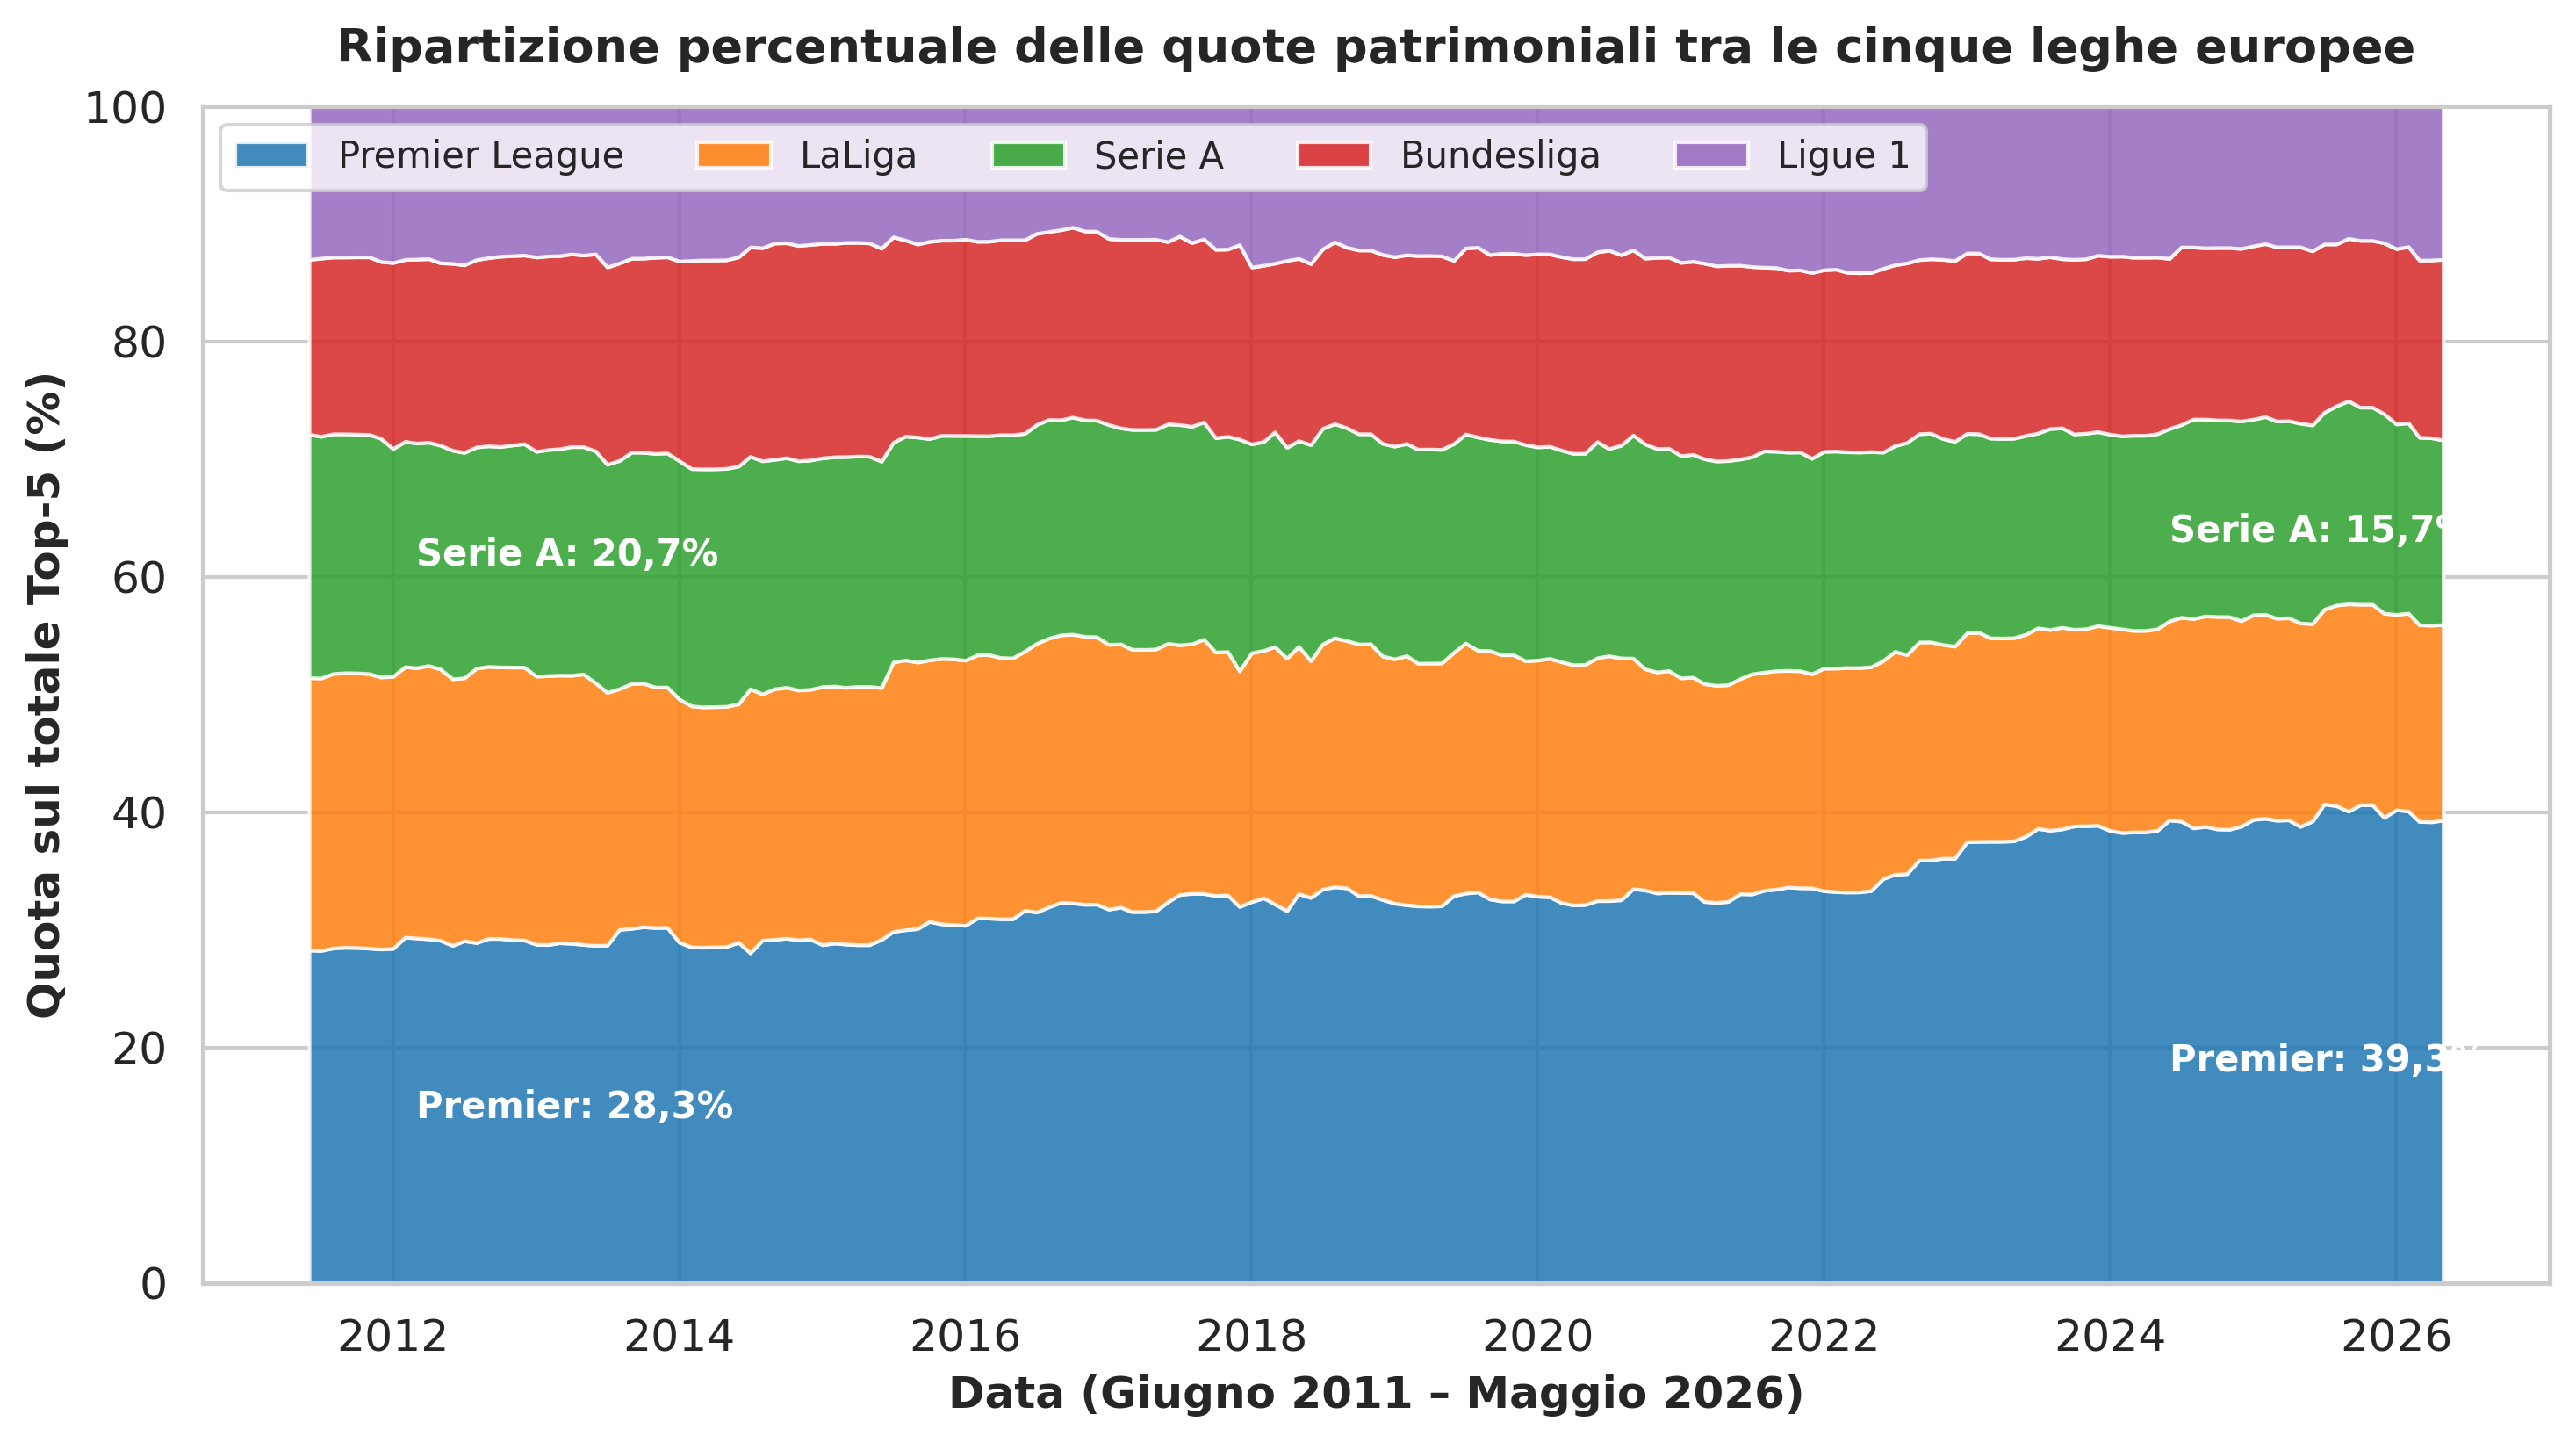
\includegraphics[width=0.95\textwidth]{capitolo7/img/fig04_eda_quote_mercato.png}
    \caption{Ripartizione percentuale delle quote patrimoniali tra le cinque leghe europee sul totale Top-5 (2011–2026).}
    \label{fig:eda_quote_mercato}
\end{figure}

Lungo i quindici anni successivi, la superiore capacità commerciale della lega inglese nella negoziazione dei diritti televisivi ha scavato un solco incolmabile: tra il 2011 e il 2026 la Premier League è cresciuta del 330,6\%, toccando un massimo assoluto di 13,87 miliardi di euro nel novembre 2025 e chiudendo a 13,55 miliardi nel maggio 2026, data in cui assorbe da sola il 39,3\% dell'intero patrimonio calcistico europeo dei Top-5 campionati (Figura \ref{fig:eda_quote_mercato}).

La Serie A italiana (\texttt{serie\_a\_market\_value\_bn}) ha invece attraversato tre fasi distinte. Nel quinquennio 2011--2015 il campionato italiano ha conosciuto una fase di sostanziale stasi, salendo lentamente da 2,30 a 2,90 miliardi di euro. Tra il 2016 e l'inizio del 2020, spinta da ingenti investimenti, la Serie A ha accelerato toccando il massimo storico di 6,08 miliardi di euro nel marzo 2020. Dopo il violento crollo pandemico, la risalita del torneo italiano si è assestata su ritmi più contenuti rispetto all'Inghilterra: nel maggio 2026 la Serie A si attesta a 5,40 miliardi di euro (quota del 15,7\% sul totale Top-5 e crescita complessiva del 134,9\%), collocandosi al terzo posto alle spalle de LaLiga (5,72 miliardi, 16,6\%) e di poco sopra alla Bundesliga (5,29 miliardi, 15,4\%).

\subsection{Anatomia dei tre shock storici: inflazione del 2017, crollo COVID-19 e ciclo post-2023}

Uno degli esiti più significativi dell'analisi della serie storica è l'individuazione di tre brusche discontinuità strutturali ben delimitate nel tempo, le quali violano l'ipotesi di crescita stazionaria uniforme e impongono l'uso di variabili indicatrici d'intervento nella modellazione predittiva.

Il primo shock strutturale coincide con l'agosto 2017 (\texttt{2017-08}), data del trasferimento record di Neymar dal Barcellona al Paris Saint-Germain per 222 milioni di euro e del rinnovo dei diritti TV internazionali. Come visualizzato nel dettaglio della Figura \ref{fig:eda_shock_neymar}, questo evento ha prodotto un immediato cambio di pendenza (\textit{slope change}) del trend economico: mentre tra giugno 2011 e luglio 2017 la serie aggregata europea cresceva a un ritmo di $+1,31$ miliardi di euro all'anno, nei trentadue mesi successivi ad agosto 2017 la crescita annualizzata è quadruplicata, toccando un tasso di $+5,46$ miliardi di euro all'anno.

\begin{figure}[H]
    \centering
    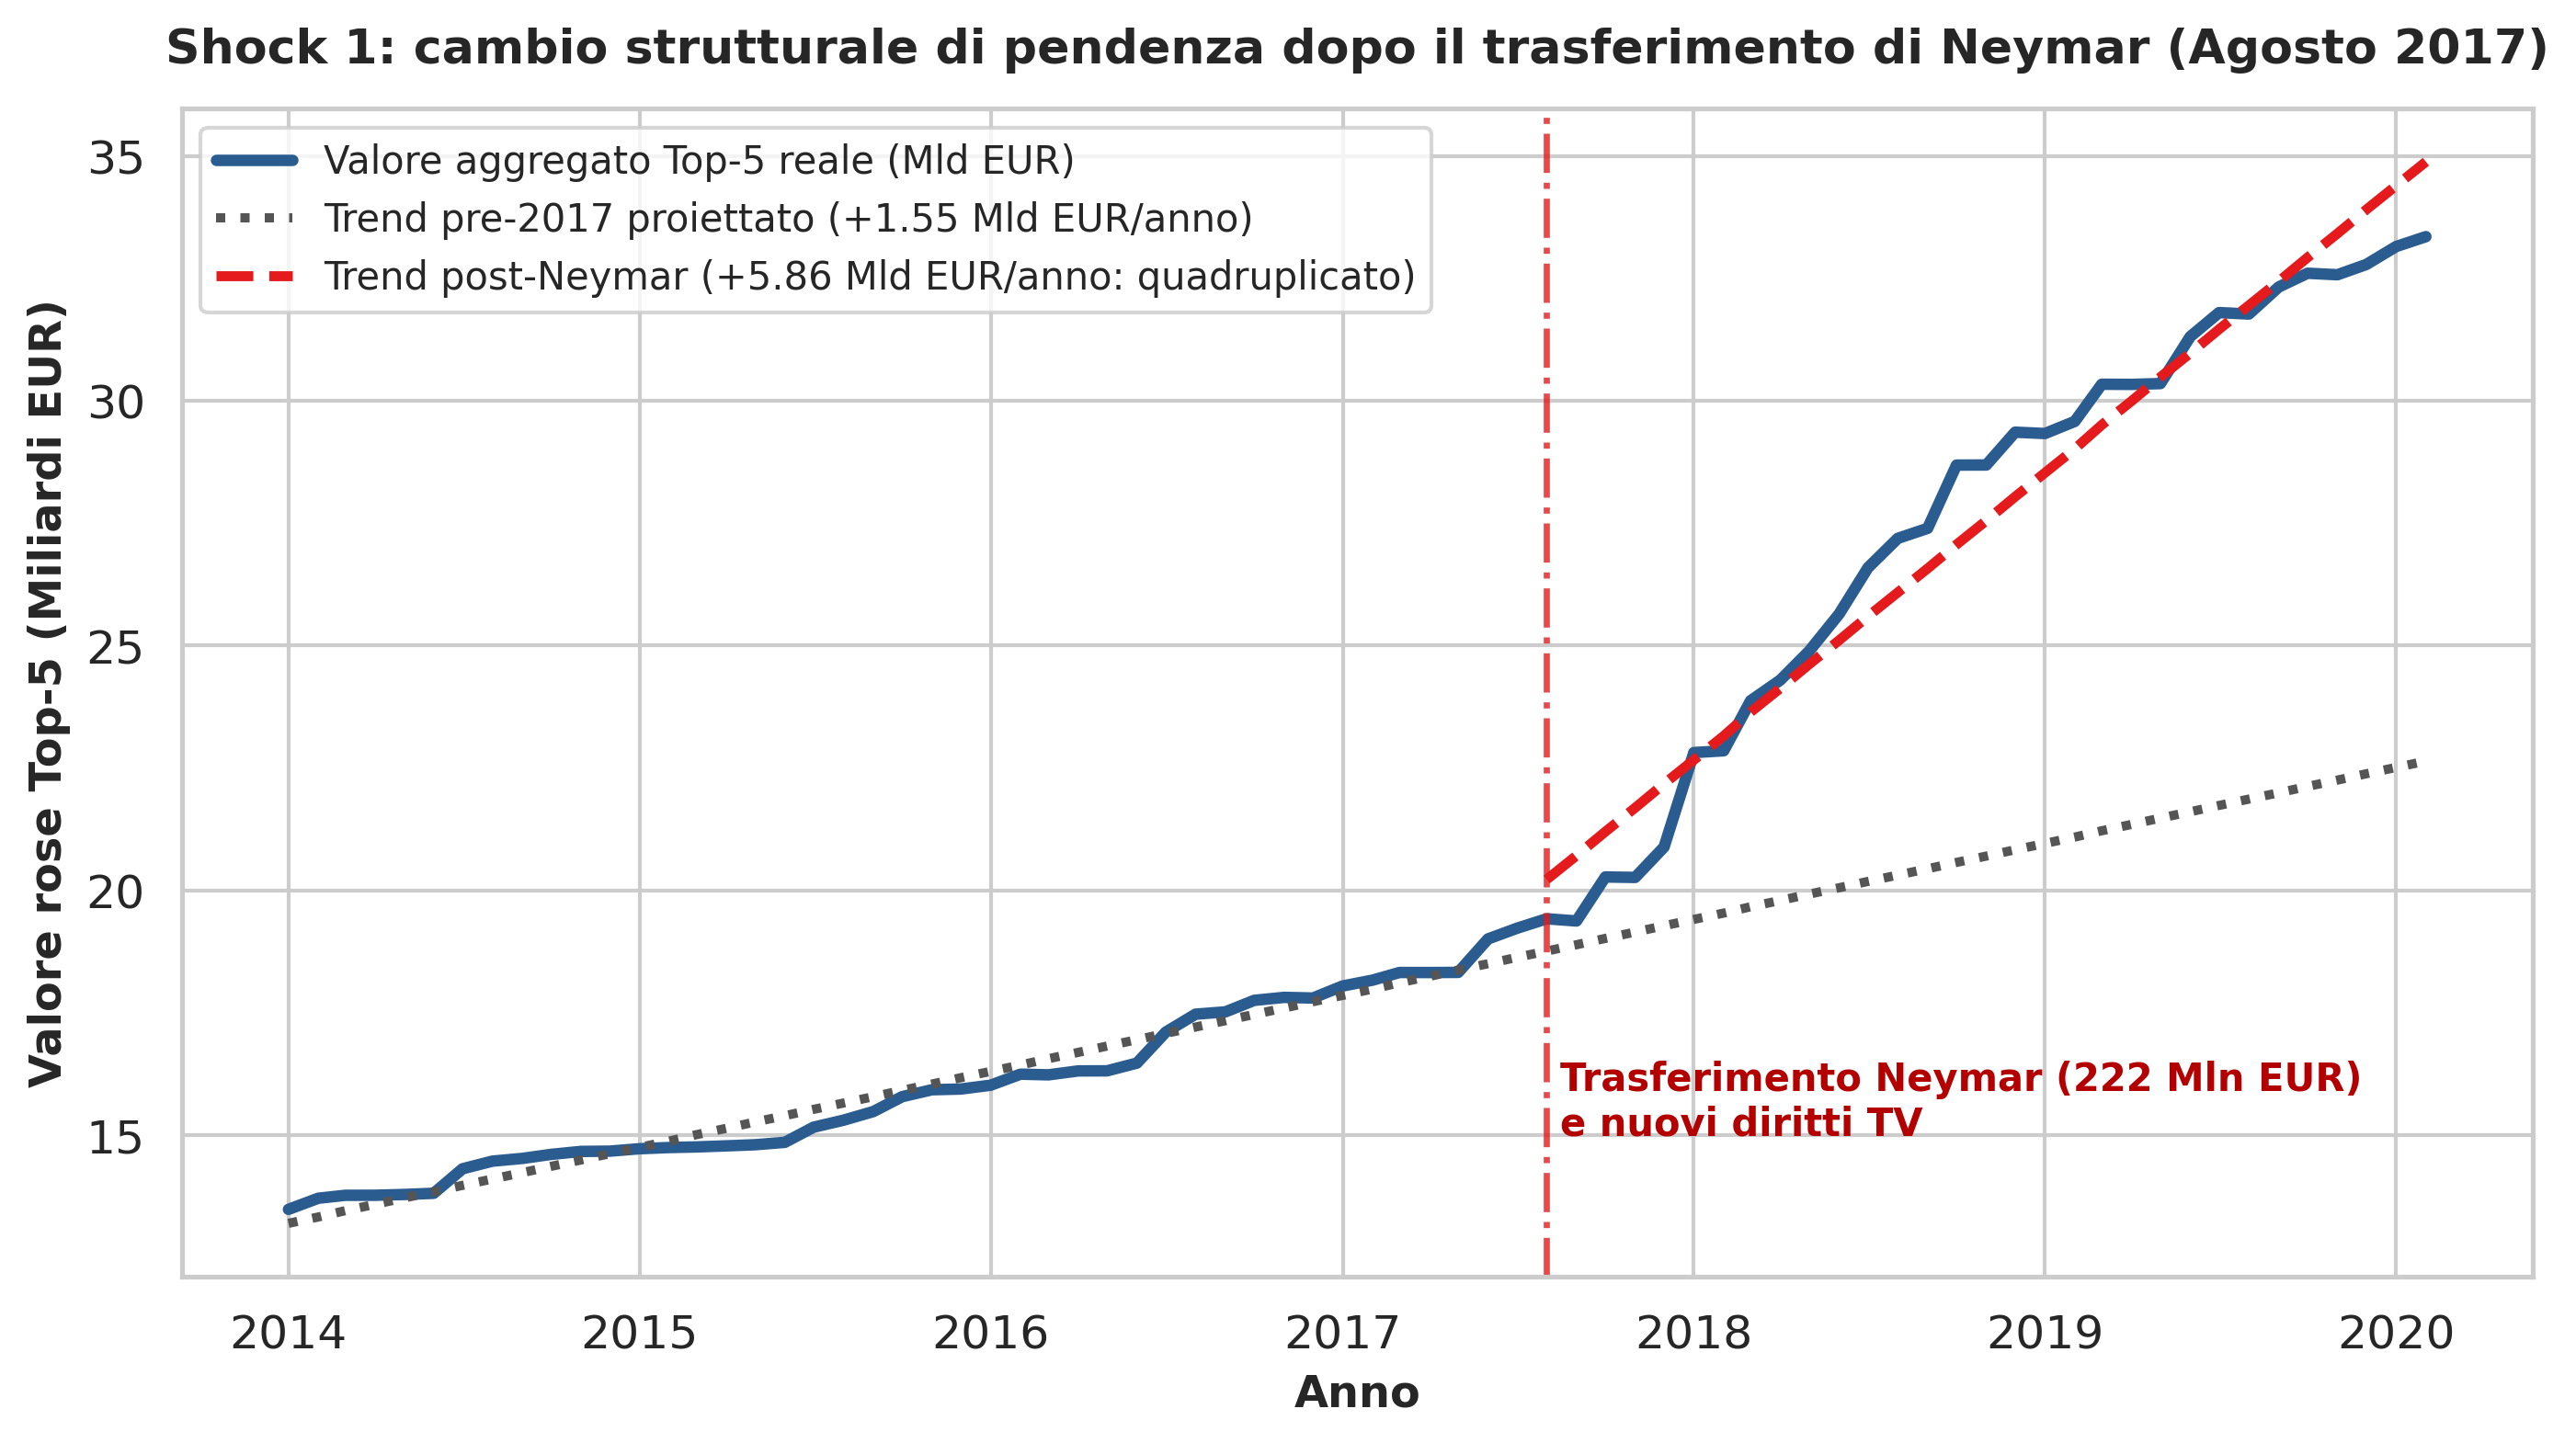
\includegraphics[width=0.92\textwidth]{capitolo7/img/fig05_eda_shock_neymar_2017.png}
    \caption{Shock 1: cambio strutturale di pendenza nel trend del valore aggregato Top-5 a seguito del trasferimento di Neymar nell'agosto 2017.}
    \label{fig:eda_shock_neymar}
\end{figure}

Il secondo shock, illustrato nella Figura \ref{fig:eda_shock_covid}, rappresenta il più drammatico evento di rottura nella storia economica del settore: l'esplosione della pandemia da COVID-19 e la sospensione totale delle competizioni sportive nella primavera del 2020. Di fronte al blocco dei ricavi da stadio e all'incertezza finanziaria, nell'aprile 2020 (\texttt{2020-04}) la piattaforma Transfermarkt ha applicato un taglio straordinario generalizzato, effettuando 4.379 ribassi di cartellino in trenta giorni. Tra marzo e aprile 2020 il valore europeo è crollato istantaneamente da 33,79 a 27,65 miliardi di euro ($-18,17\%$, con una perdita secca di 6,14 miliardi di euro), mentre la Serie A è precipitata da 6,08 a 4,97 miliardi ($-18,34\%$). Come evidenziato dalla linea tratteggiata del picco pre-pandemico, la serie ha impiegato esattamente 55 mesi (oltre quattro anni e mezzo) per ritornare ai livelli pre-crisi, superando nuovamente la soglia dei 33,79 miliardi solo nell'ottobre 2024 (33,83 miliardi di euro).

\begin{figure}[H]
    \centering
    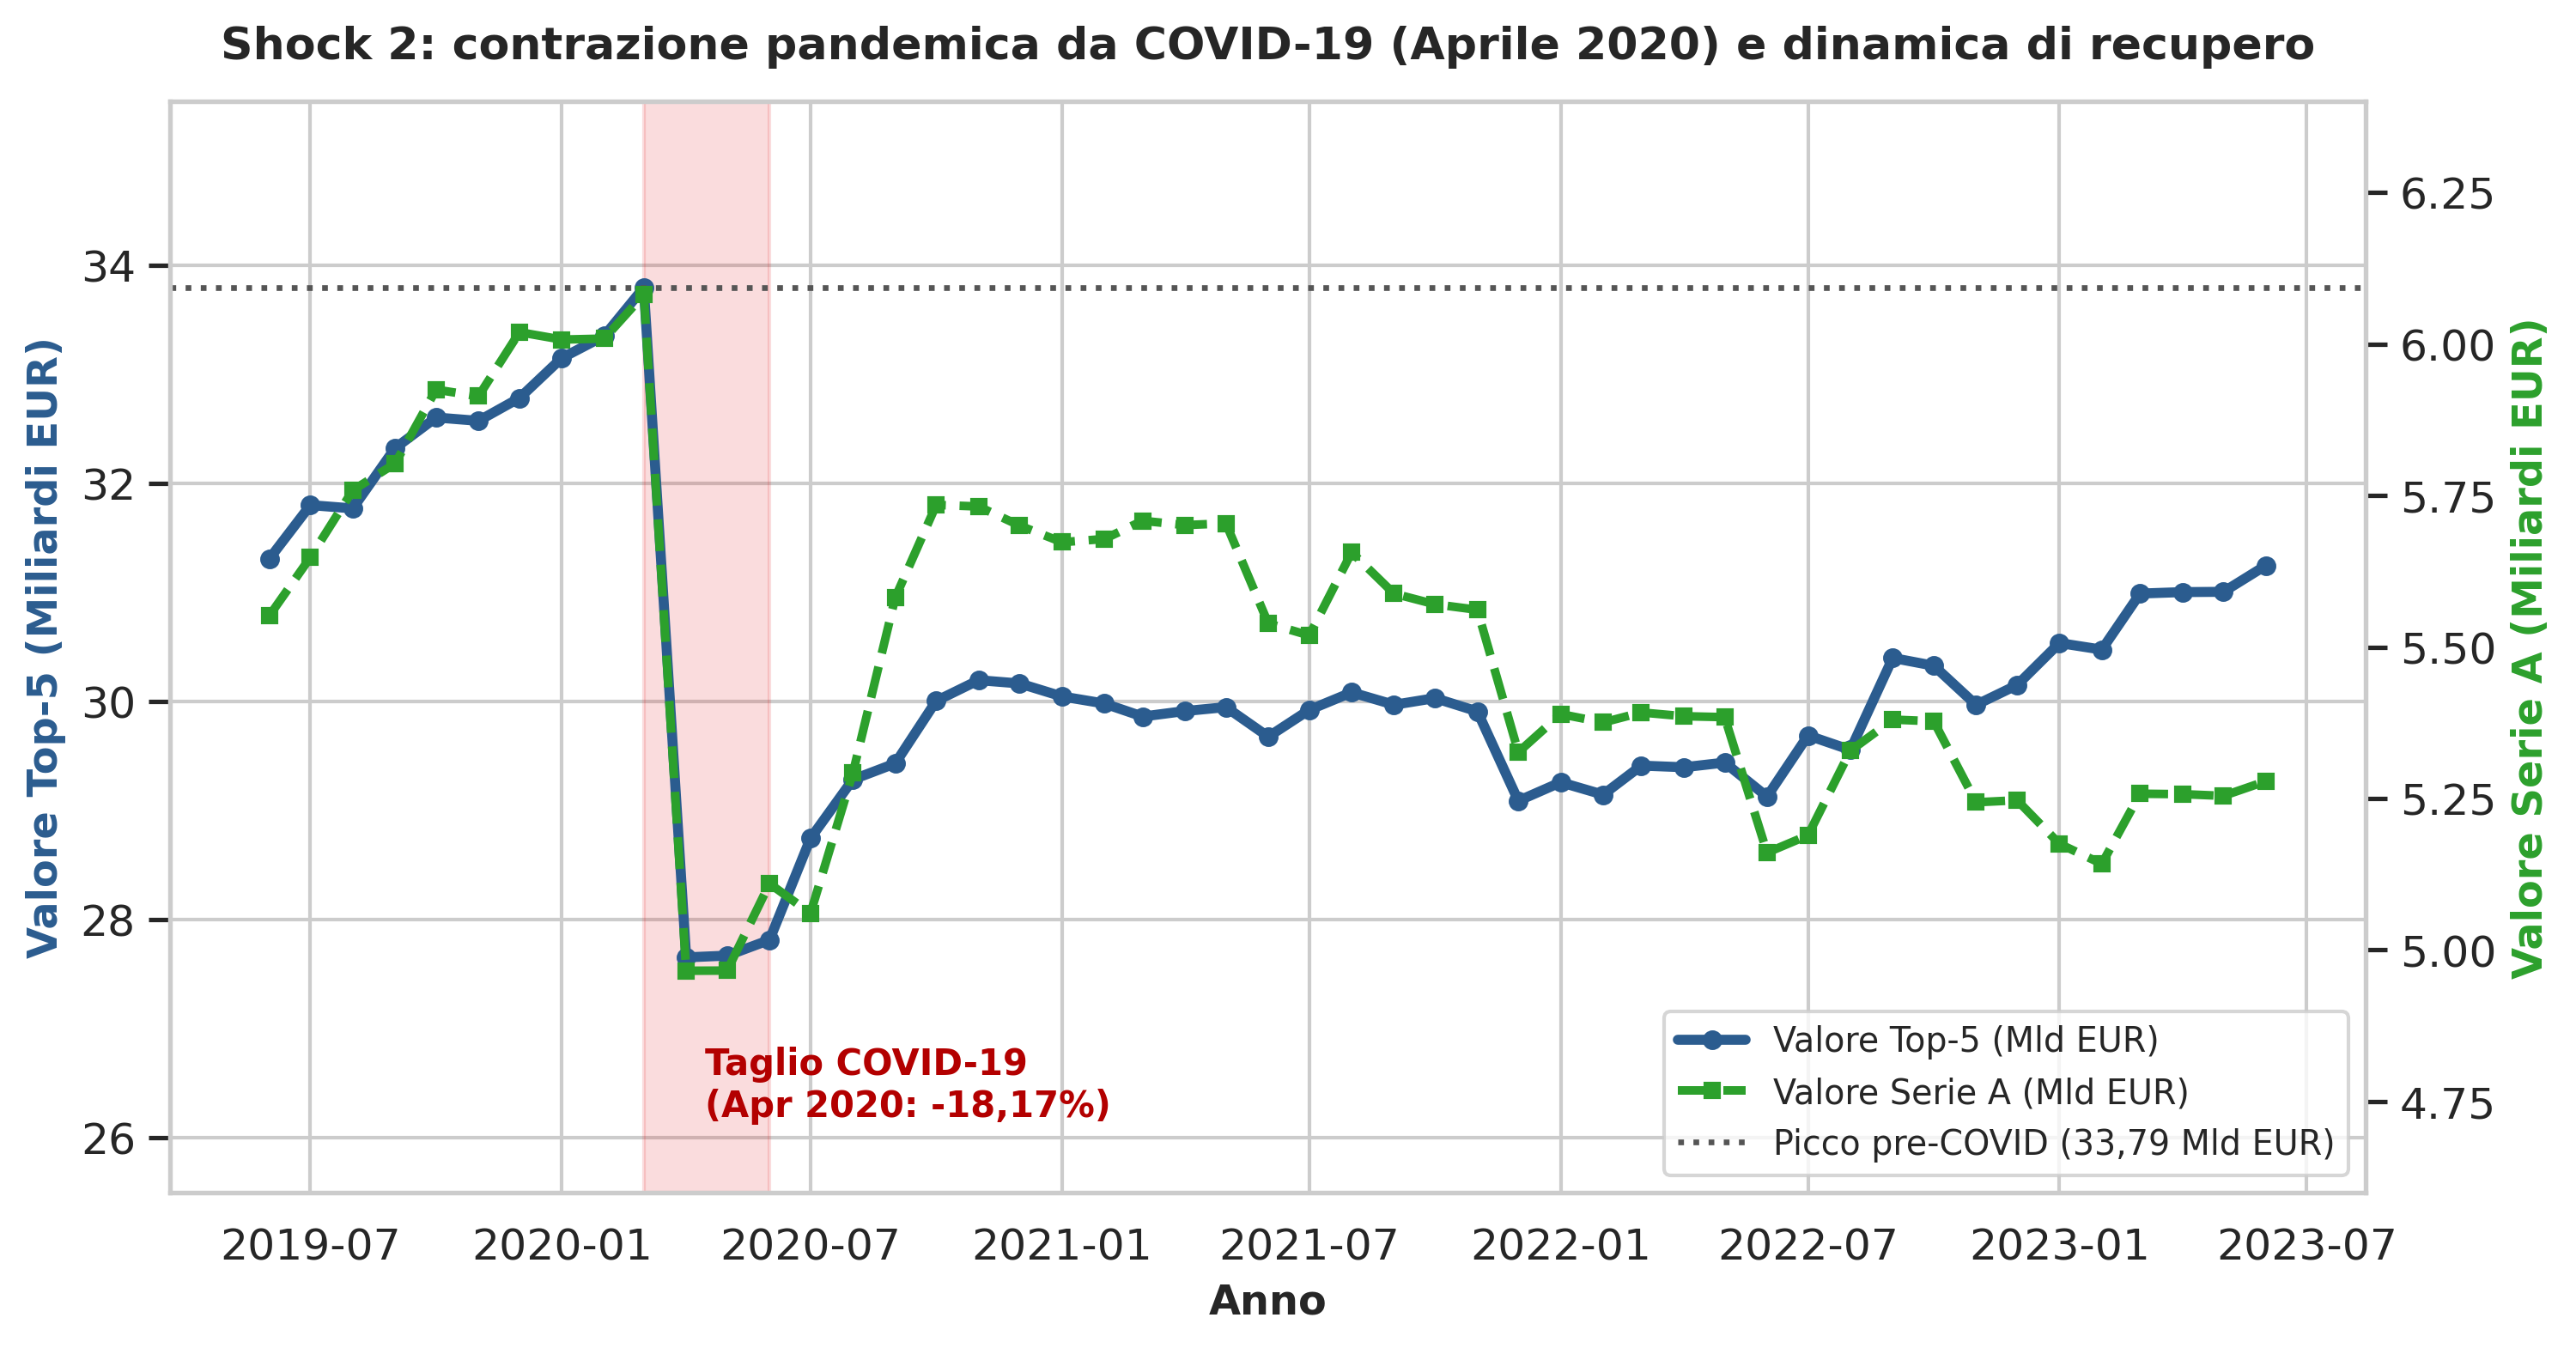
\includegraphics[width=0.92\textwidth]{capitolo7/img/fig06_eda_shock_covid_2020.png}
    \caption{Shock 2: contrazione pandemica da COVID-19 nell'aprile 2020 ($-18,17\%$) e dinamica temporale di recupero del valore patrimoniale.}
    \label{fig:eda_shock_covid}
\end{figure}

Il terzo fenomeno strutturale, mostrato nella Figura \ref{fig:eda_shock_boom}, descrive la forte ripartenza del triennio 2023--2026, sostenuta dall'irruzione finanziaria della Saudi Pro League nell'estate 2023 e dall'entrata in vigore del nuovo format allargato della UEFA Champions League a partire dalla stagione 2024/2025. Tale fase conduce la serie al massimo storico assoluto di 34,44 miliardi di euro nel maggio 2026 e si caratterizza per una massiccia rivalutazione dei cartellini dei calciatori di vertice: il valore medio per giocatore attivo (\texttt{mean\_player\_value\_m}), rimasto attorno ai 3 milioni di euro fino al 2017 e pari a 5,07 milioni nel marzo 2020, accelera fino a superare la soglia degli 11 milioni di euro (11,01 milioni) nella primavera del 2026.

\begin{figure}[H]
    \centering
    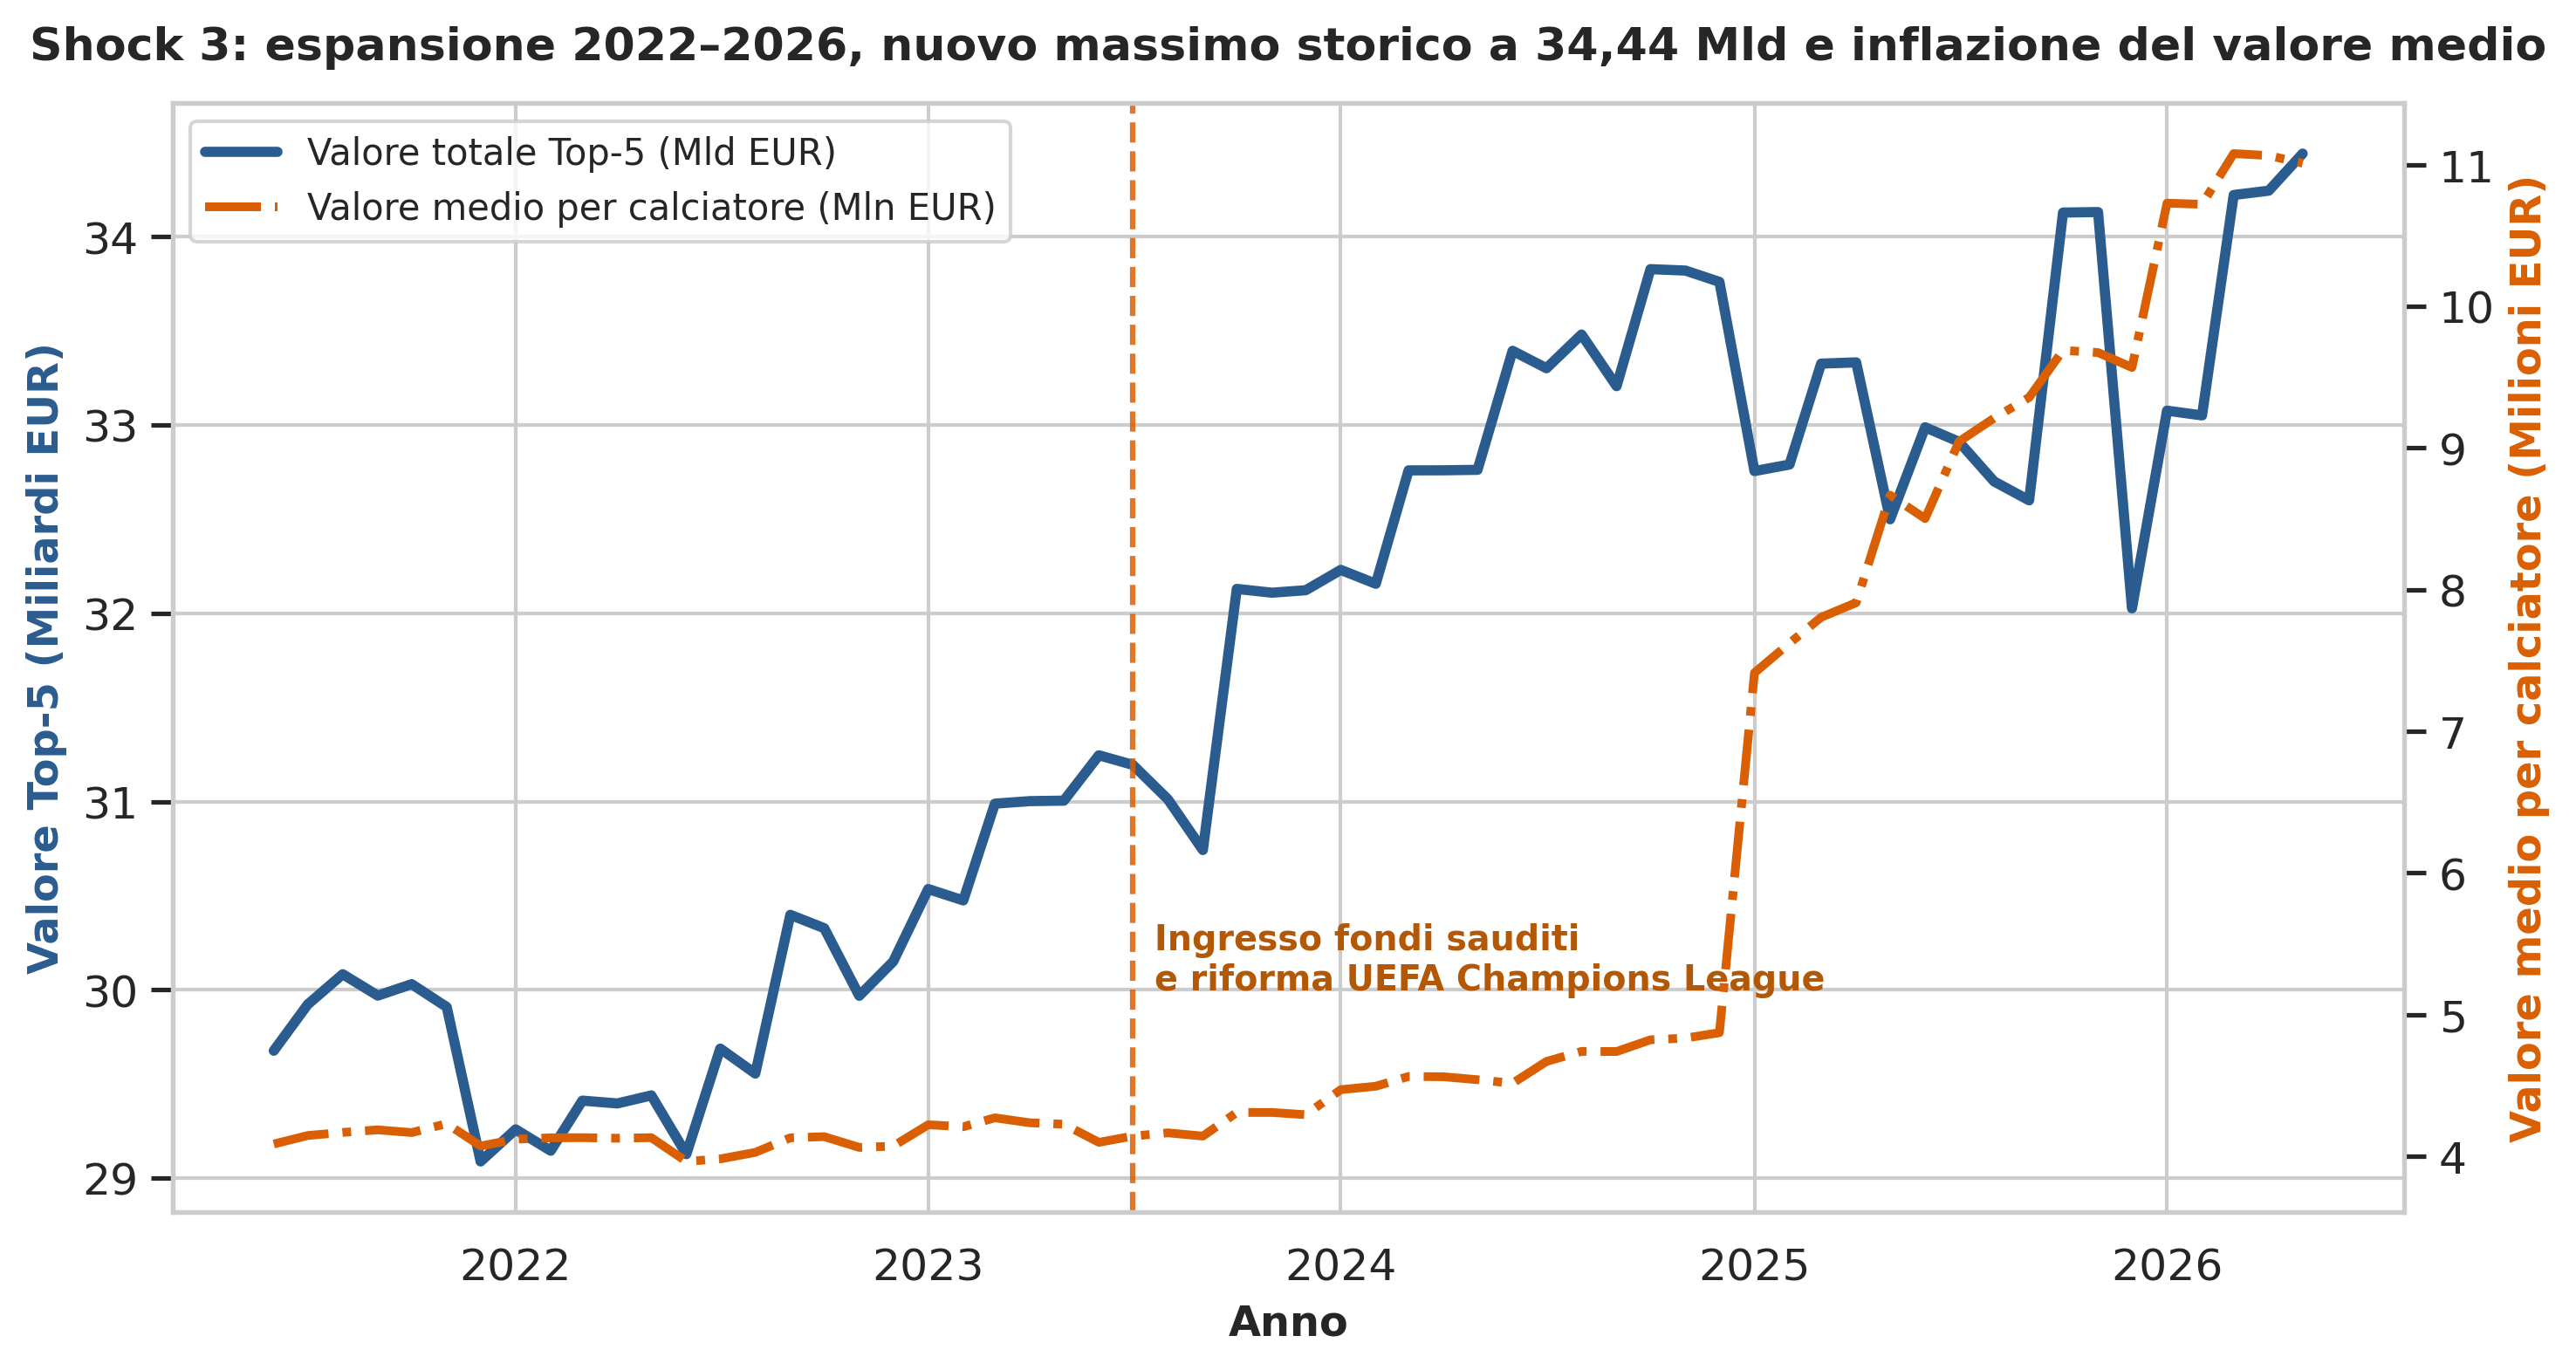
\includegraphics[width=0.92\textwidth]{capitolo7/img/fig07_eda_shock_boom_2026.png}
    \caption{Shock 3: espansione post-2023, nuovo massimo storico a 34,44 miliardi di euro e impennata del valore medio per giocatore.}
    \label{fig:eda_shock_boom}
\end{figure}

\subsection{Analisi delle variazioni percentuali mensili, volatilità e identificazione degli outlier}

Per analizzare il comportamento dinamico della serie al netto del trend di fondo, è stata calcolata la serie delle variazioni percentuali mensili (\textit{Change \%}):
\begin{equation}
    \Delta\%_t = \frac{Y_t - Y_{t-1}}{Y_{t-1}} \cdot 100
    \label{eq:pct_change}
\end{equation}
dove $Y_t$ indica il valore aggregato al mese $t$. Nella Figura \ref{fig:eda_change_pct} viene riportato l'andamento nel tempo di $\Delta\%_t$ con l'evidenziazione delle bande di variabilità naturale $\mu \pm 2\sigma$.

\begin{figure}[H]
    \centering
    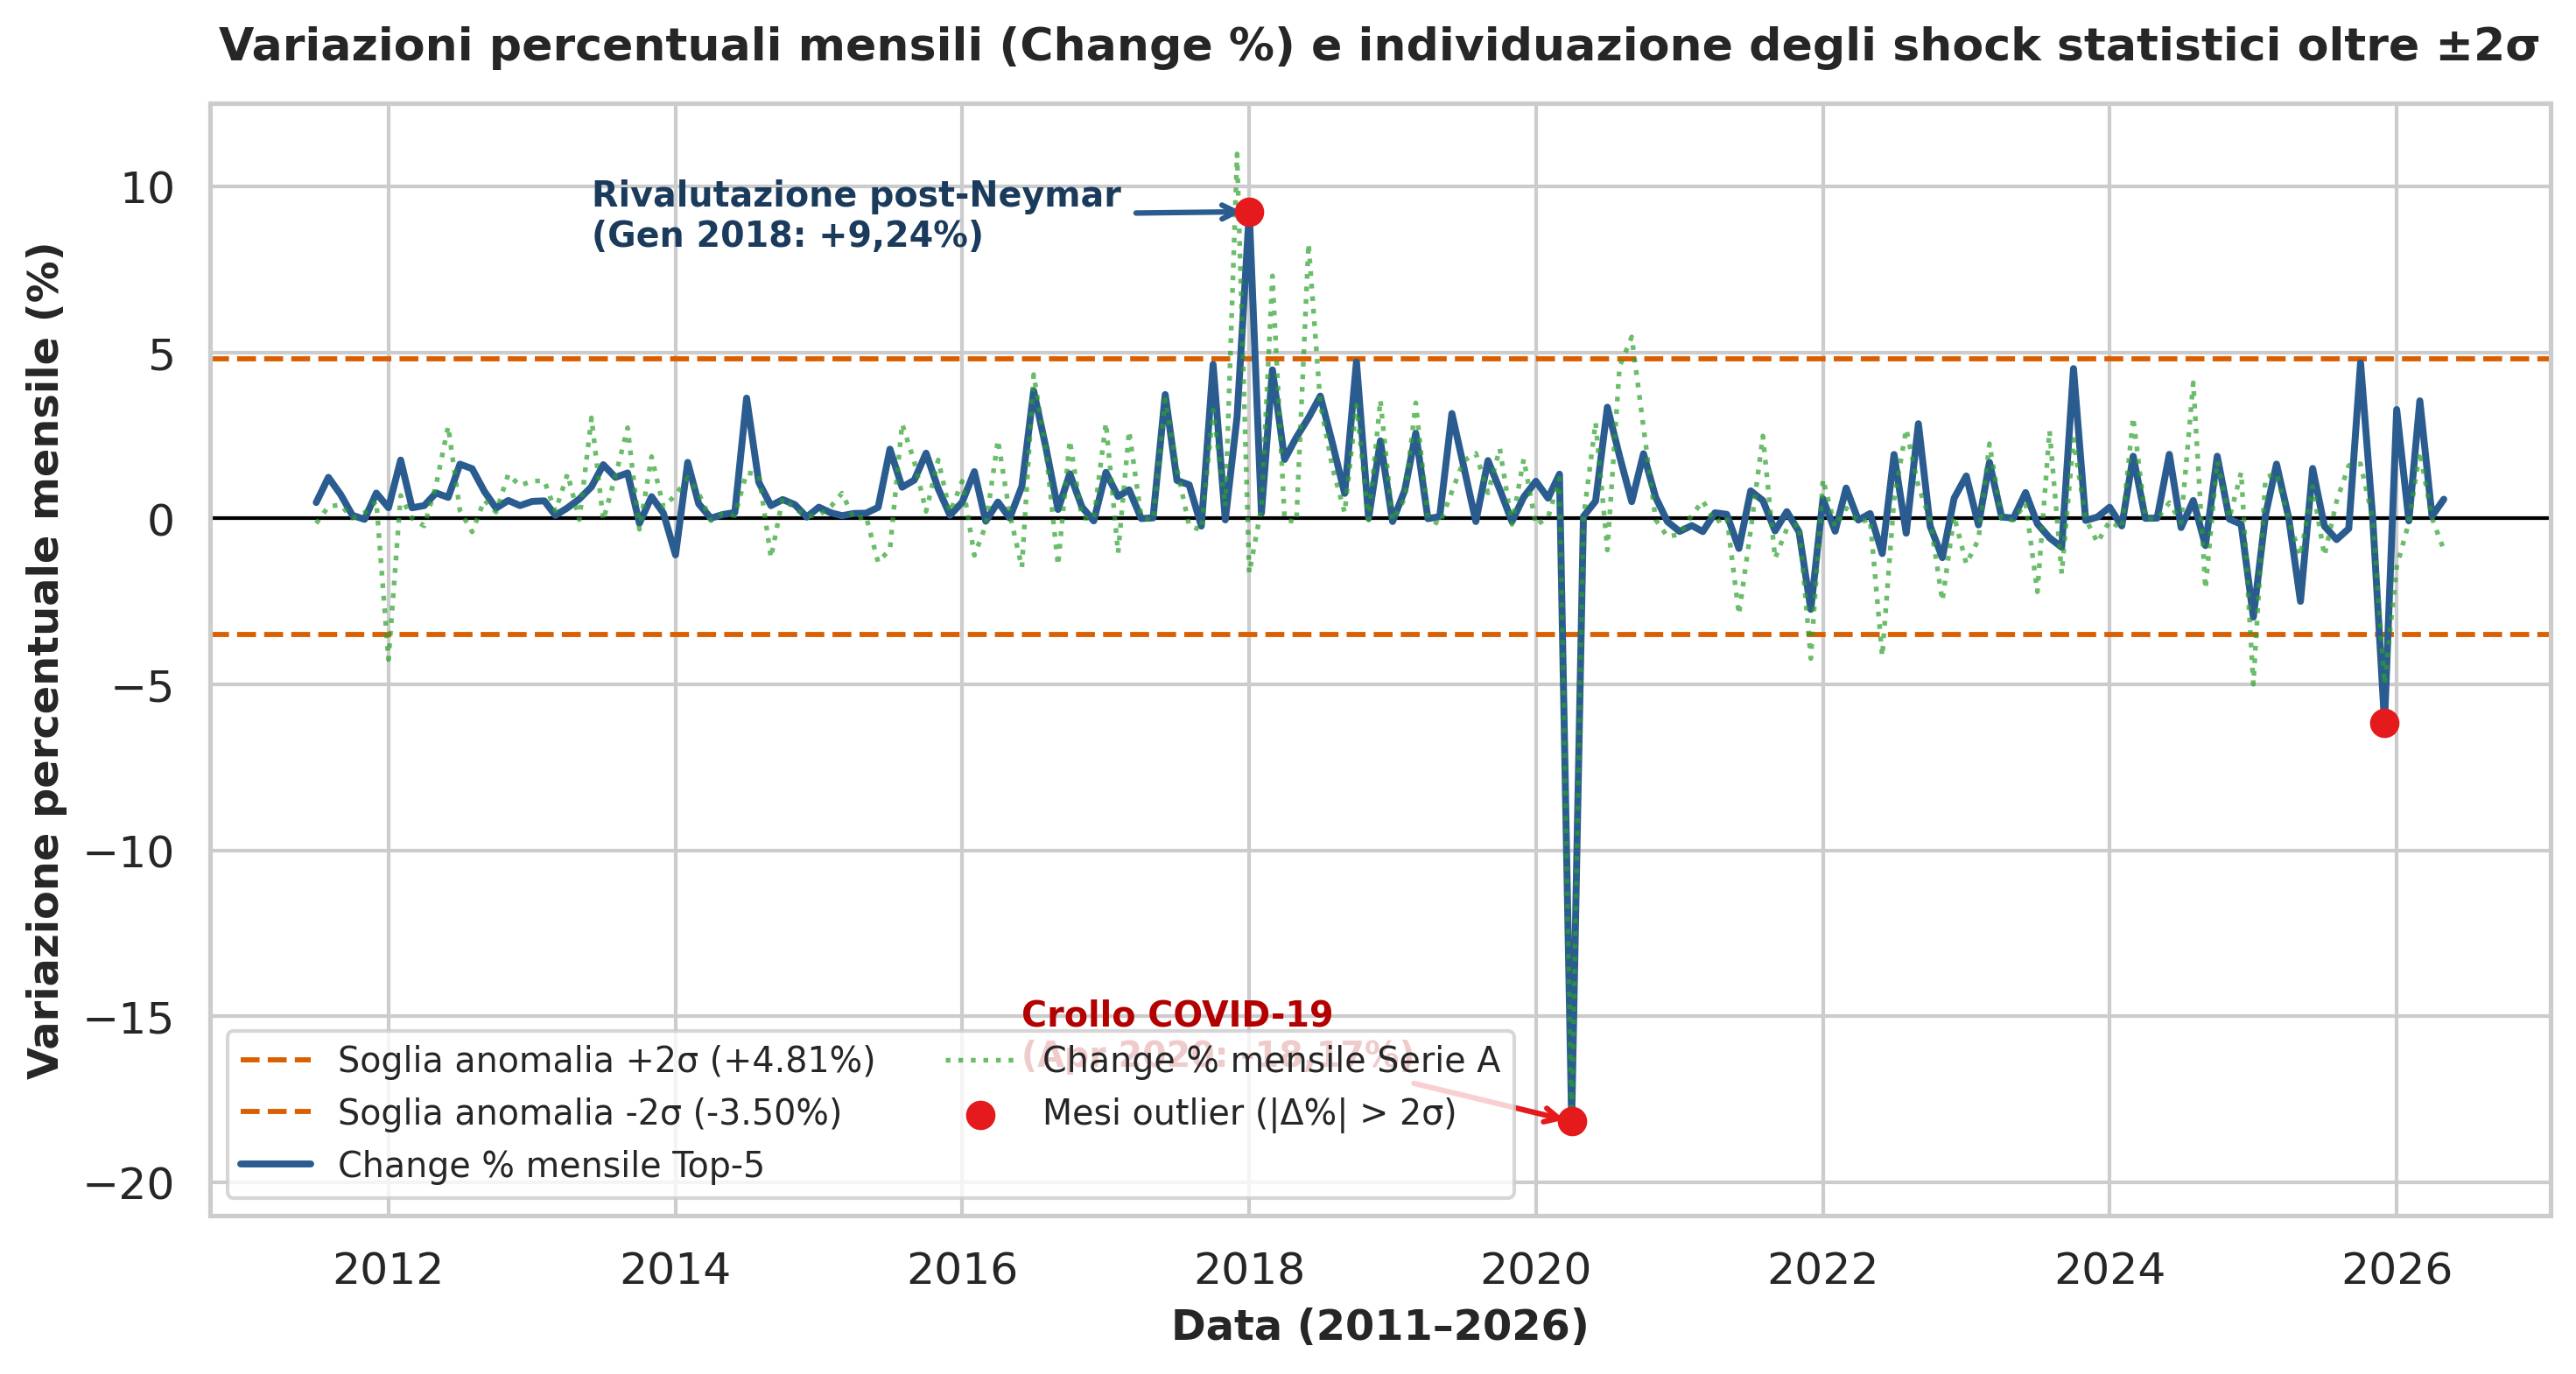
\includegraphics[width=0.95\textwidth]{capitolo7/img/fig08_eda_change_pct_volatilita.png}
    \caption{Serie storica delle variazioni percentuali mensili con fasce di confidenza $\pm 2\sigma$ e identificazione dei punti anomali.}
    \label{fig:eda_change_pct}
\end{figure}

Sull'arco delle 179 variazioni mensili tra luglio 2011 e maggio 2026, la variazione media mensile si attesta a $\mu = +0,66\%$ con una deviazione standard pari a $\sigma = 2,06\%$, definendo una fascia tipica $[\mu - 2\sigma, \, \mu + 2\sigma]$ compresa tra $-3,46\%$ e $+4,78\%$. Come visibile nella Figura \ref{fig:eda_change_pct}, l'applicazione del criterio $| \Delta\%_t - \mu | > 2\sigma$ permette di isolare con rigore statistico gli shock esogeni: il picco massimo si colloca nel gennaio 2018 ($+9,24\%$, a seguito dell'adeguamento generale dei listini post-Neymar), mentre il valore minimo coincide con il crollo pandemico di aprile 2020 ($-18,17\%$, un evento eccezionale a oltre nove deviazioni standard dalla media, $z = -9,14$).

La forma distributiva di tali variazioni è analizzata nella Figura \ref{fig:eda_distribuzione_kde} attraverso la stima di densità kernel (KDE).

\begin{figure}[H]
    \centering
    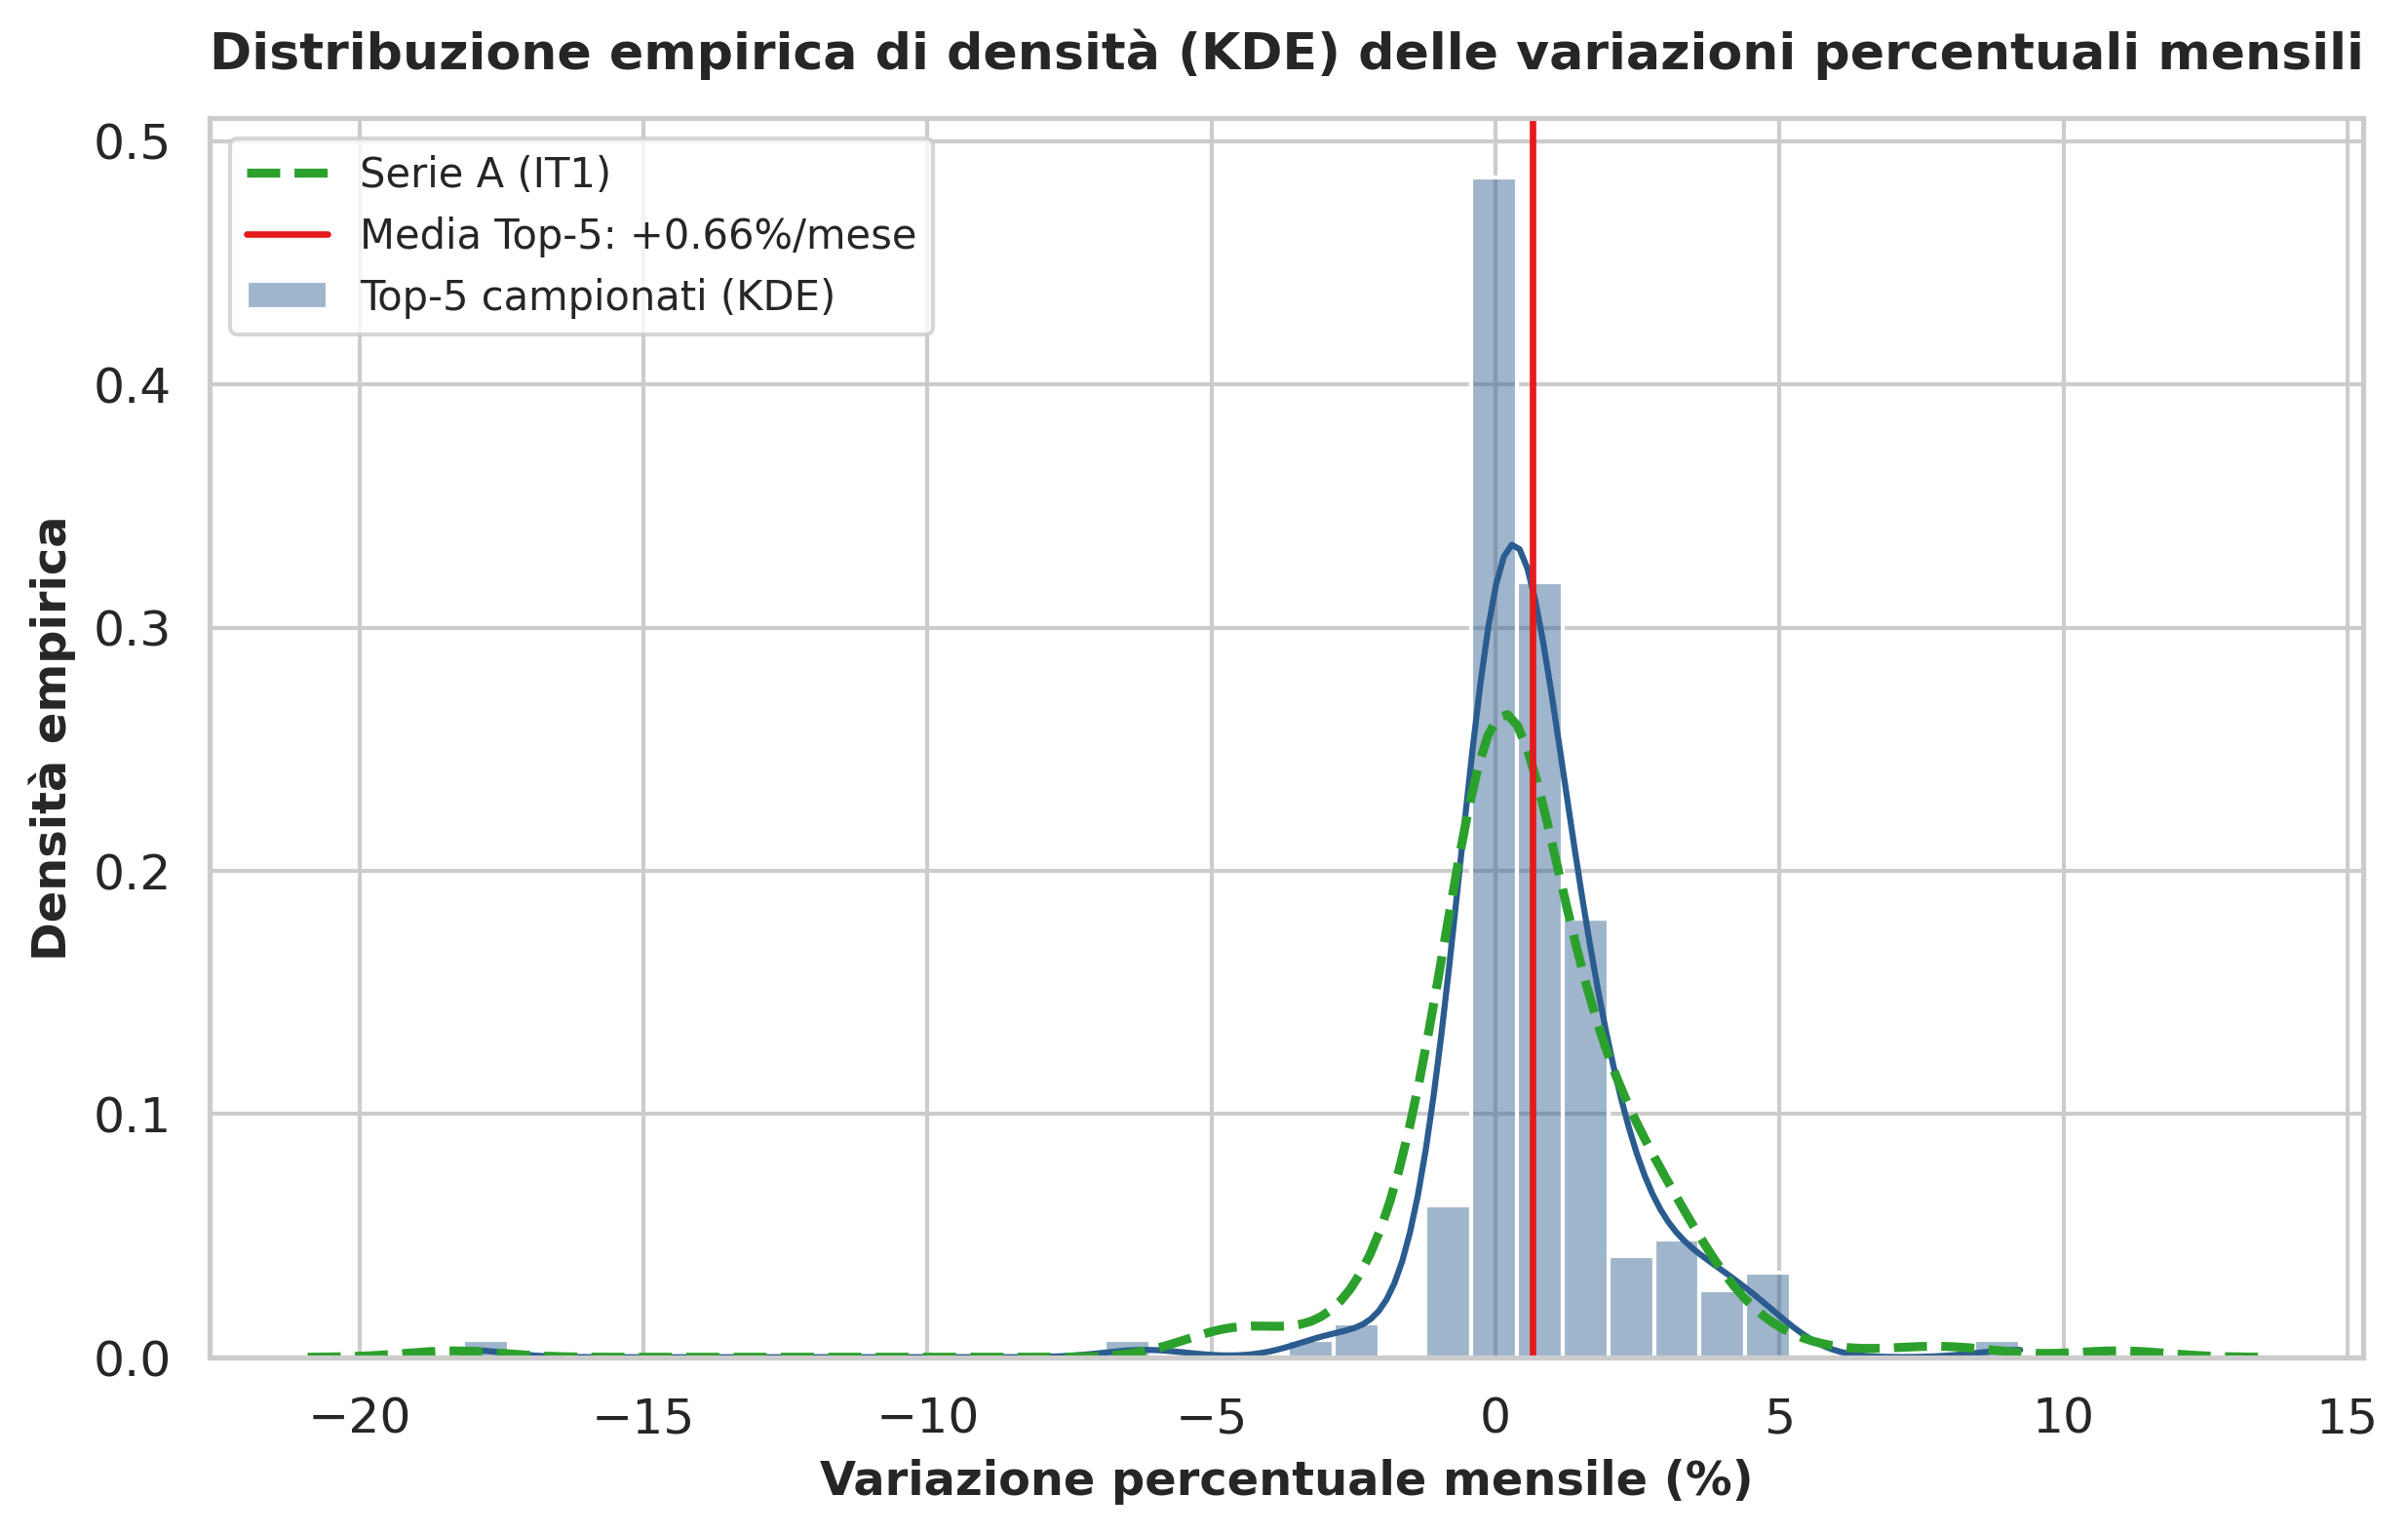
\includegraphics[width=0.88\textwidth]{capitolo7/img/fig09_eda_distribuzione_kde.png}
    \caption{Distribuzione empirica di densità (KDE) e istogramma delle variazioni percentuali mensili per i Top-5 campionati e la Serie A.}
    \label{fig:eda_distribuzione_kde}
\end{figure}

Come confermato dalla Figura \ref{fig:eda_distribuzione_kde}, la presenza di scossoni localizzati conferisce alla curva empirica una spiccata asimmetria negativa (\textit{skewness} pari a $-3,69$) e un'elevata curtosi (\textit{kurtosis} in eccesso pari a $35,48$, tipica di serie temporali con code pesanti e salti repentini). Inoltre, la Serie A (curva verde) manifesta una dispersione leggermente più ampia ($\sigma_{\text{IT1}} = 2,52\%$), dovuta al fatto che le contrattazioni e le rivalutazioni di una singola federazione nazionale risentono maggiormente della stagionalità del calendario rispetto all'aggregato europeo.

\subsection{Relazione dinamica tra valore delle rose e spese nelle sessioni di calciomercato}

L'ultimo asse d'indagine dell'analisi esplorativa studia il legame tra la serie di consistenza patrimoniale delle rose (\texttt{top5\_market\_value\_bn}) e i flussi monetari effettivi generati dal calciomercato (\texttt{transfer\_spend\_top5\_m}). Nel quindicennio considerato, i club delle cinque leghe hanno effettuato 31.000 trasferimenti in ingresso (di cui 8.105 a titolo oneroso), mobilitando una spesa cumulata di 65,82 miliardi di euro (di cui 14,68 miliardi spesi dalla sola Serie A, pari al 22,3\% del totale europeo).

Nella Figura \ref{fig:eda_spese_impulsi} viene confrontata la traiettoria del valore delle rose con gli impulsi mensili di spesa per trasferimenti.

\begin{figure}[H]
    \centering
    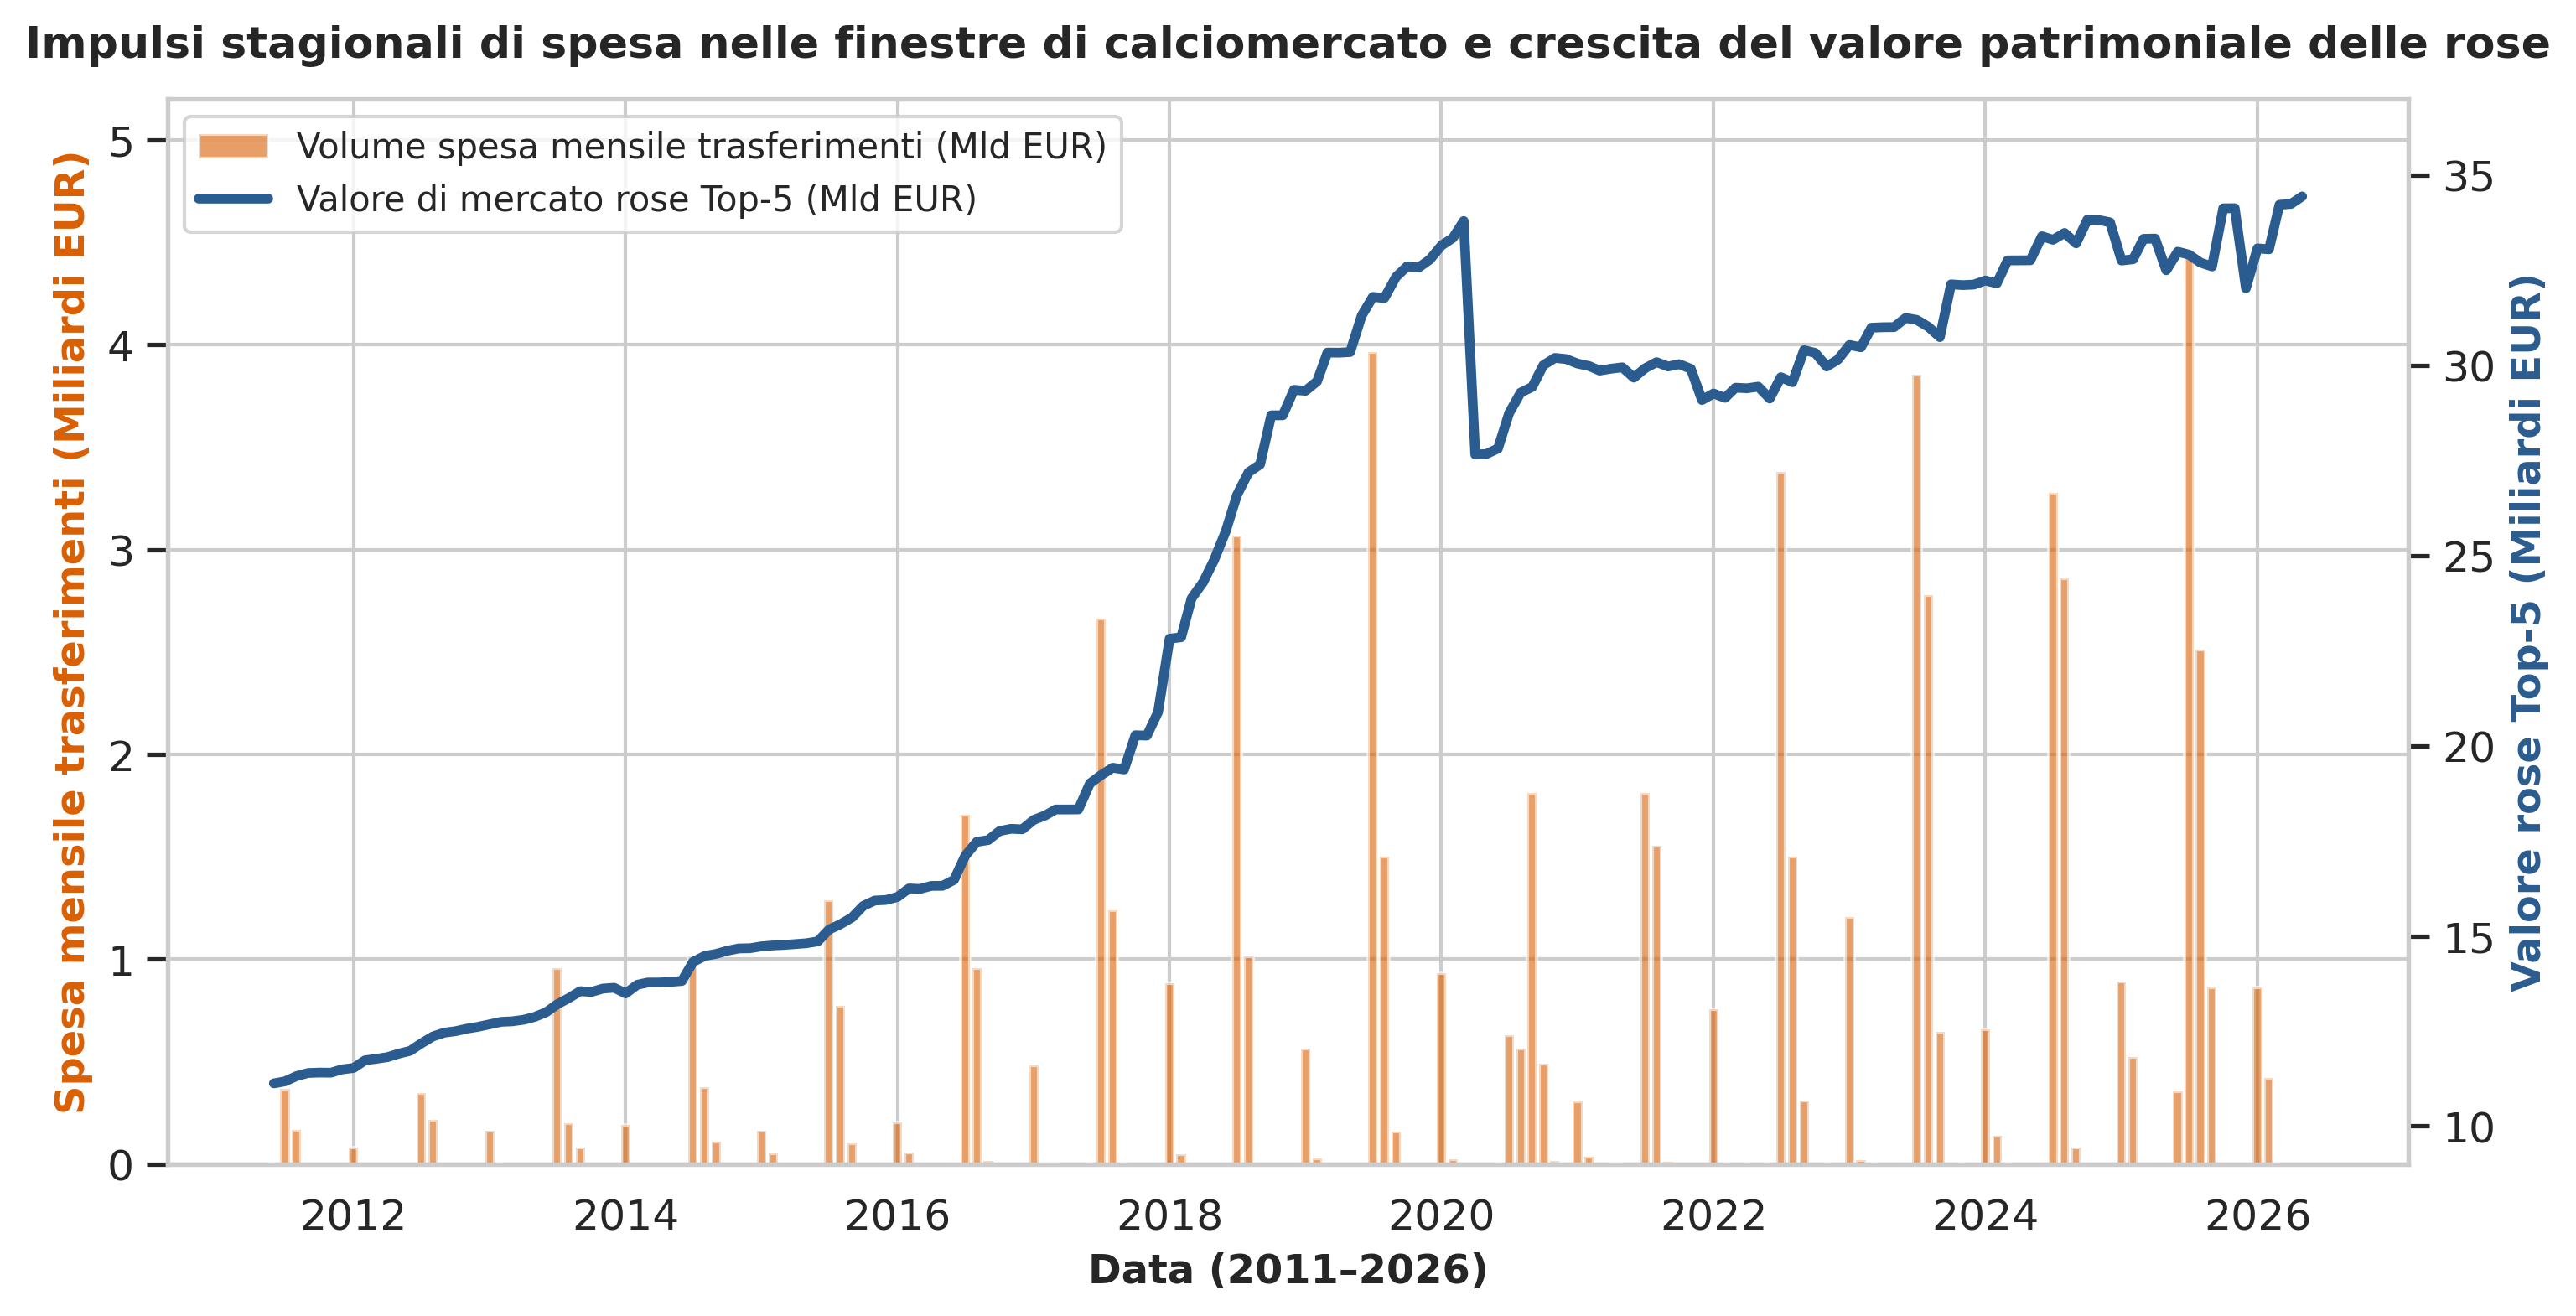
\includegraphics[width=0.95\textwidth]{capitolo7/img/fig10_eda_spese_calciomercato_impulsi.png}
    \caption{Impulsi stagionali di spesa nelle sessioni di calciomercato e crescita del valore patrimoniale delle rose (2011–2026).}
    \label{fig:eda_spese_impulsi}
\end{figure}

La Figura \ref{fig:eda_spese_impulsi} mette in risalto la marcata stagionalità della spesa per trasferimenti: i volumi monetari si concentrano quasi per intero nei mesi di luglio e agosto, con una finestra secondaria a gennaio, risultando quasi azzerati nei mesi restanti. Inoltre, l'altezza degli impulsi estivi cresce parallelamente all'espansione economica del settore: dai 533 milioni di euro dell'estate 2011 si giunge ai 3,90 miliardi dell'estate 2017 e ai 5,47 miliardi del 2019, fino a toccare il record assoluto nel luglio 2025 con 4.457,95 milioni di euro spesi in un solo mese (di cui 1.128,06 milioni in Serie A).

Per quantificare matematicamente la forza di questo legame, la Figura \ref{fig:eda_matrice_corr} riporta la matrice di correlazione lineare di Pearson tra le variabili patrimoniali e le grandezze di mercato.

\begin{figure}[H]
    \centering
    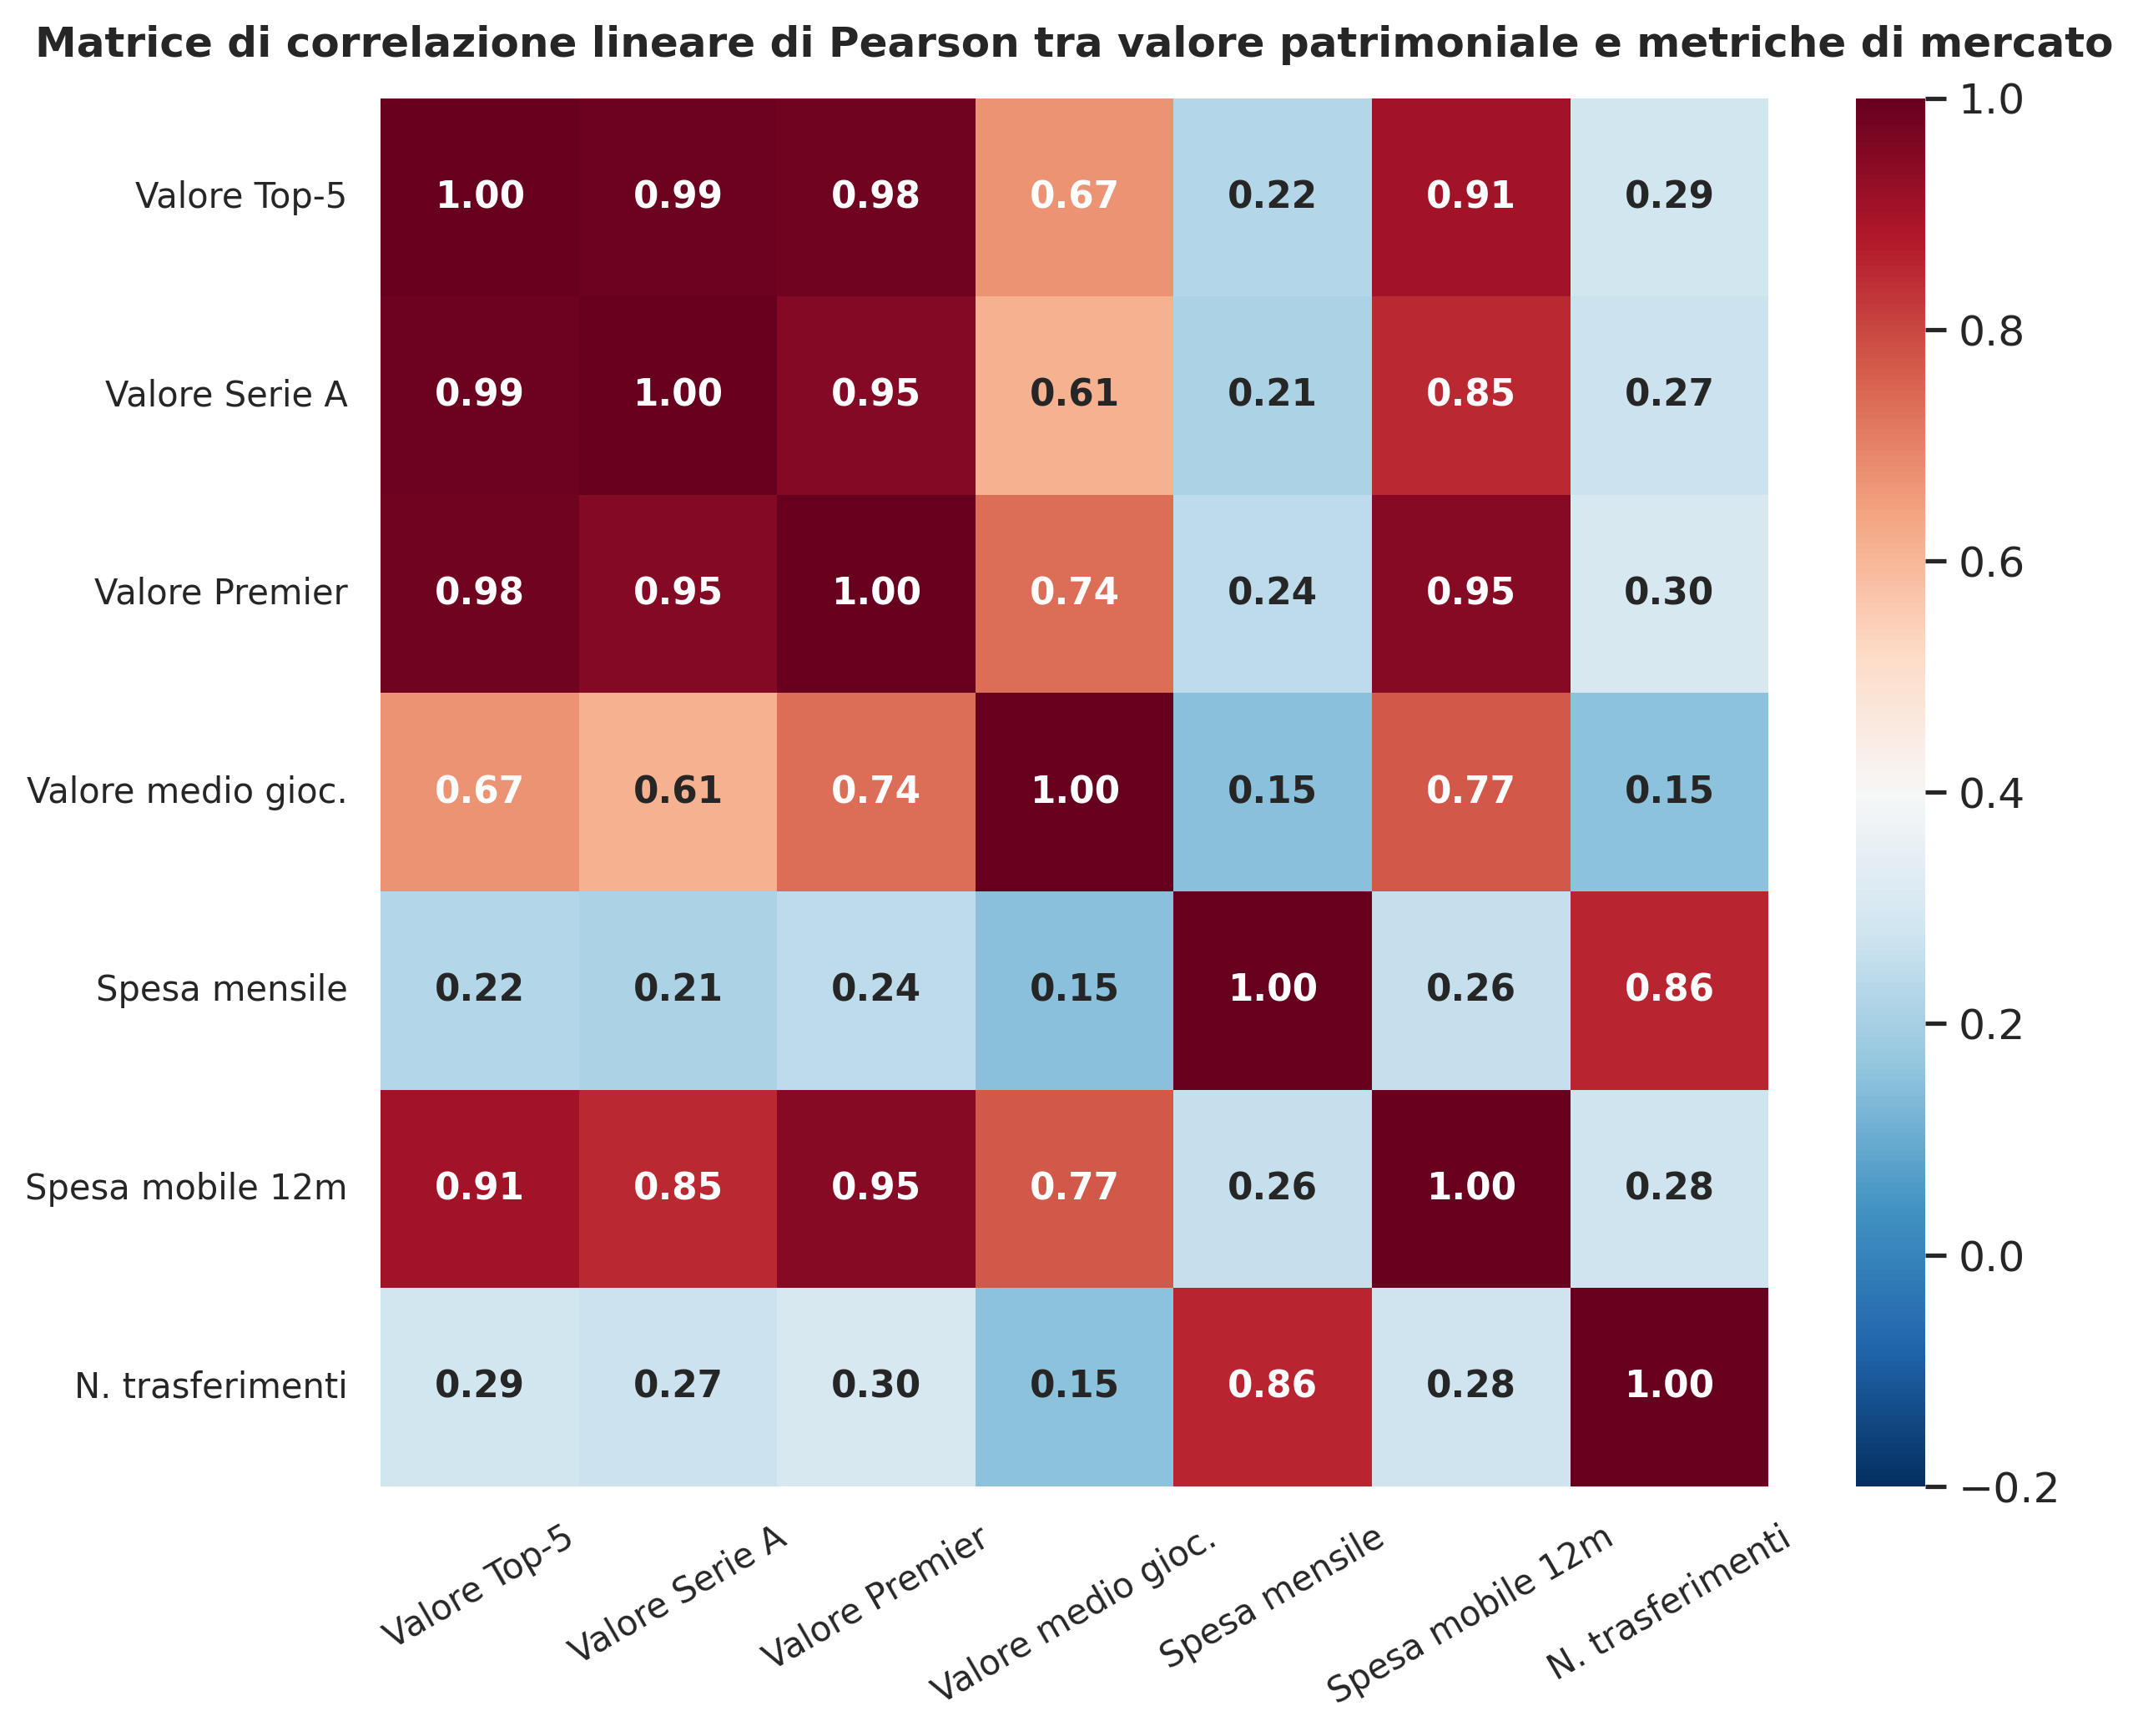
\includegraphics[width=0.85\textwidth]{capitolo7/img/fig11_eda_matrice_correlazione.png}
    \caption{Matrice di correlazione lineare di Pearson tra valore patrimoniale delle rose e metriche di spesa del calciomercato.}
    \label{fig:eda_matrice_corr}
\end{figure}

Dalla matrice di correlazione in Figura \ref{fig:eda_matrice_corr} emerge un'evidenza metodologica cruciale: la correlazione puntuale tra il valore delle rose e la spesa del singolo mese è pari a $r = 0,24$ (poiché la spesa si concentra in soli tre mesi mentre le rose mantengono valore tutto l'anno); tuttavia, non appena si considera la spesa cumulata mobile sui dodici mesi precedenti (\texttt{Spesa mobile 12m}), la correlazione con il valore aggregato Top-5 schizza a $r = 0,88$ ($r = 0,92$ con la Premier League e $r = 0,80$ con la Serie A). 

Tale risultato certifica che la liquidità immessa nel calciomercato durante l'anno costituisce la determinante economica primaria dell'inflazione del valore delle squadre, validando pienamente la scelta di impiegare la spesa e il numero di trasferimenti come predittori esogeni nei modelli SARIMAX del Capitolo 9.

\newpage
% =========================================================================
% CAPITOLO 8: DECOMPOSIZIONE STAGIONALE, STAZIONARIETA E IDENTIFICAZIONE
% (Da completare nello Step 3)
% =========================================================================
\section{Decomposizione stagionale, stazionarieta e analisi delle autocorrelazioni}
\label{sec:stl_stazionarieta}

Il presente capitolo è dedicato all'analisi della struttura temporale della serie mediante decomposizione STL con periodo stagionale annuale ($s = 12$). Vengono illustrati i risultati formali dei test di radice unitaria (Augmented Dickey-Fuller e KPSS) per verificare la non stazionarietà della serie originaria e la sua riconduzione a stazionarietà mediante differenziazione prima. L'analisi è completata dall'ispezione dei correlogrammi di autocorrelazione semplice (ACF) e parziale (PACF) per la selezione degli ordini autoregressivi e di media mobile.


\newpage
% =========================================================================
% CAPITOLO 9: MODELLAZIONE PREDITTIVA, FOCUS SERIE A E CONCLUSIONI FINALI
% =========================================================================
\section{Modellazione predittiva, focus sulla Serie A e conclusioni}

L'ultima fase del percorso di ricerca dedicato alle serie storiche traduce le evidenze emerse durante l'ingegneria dei dati (Capitolo 6), l'analisi esplorativa degli shock (Capitolo 7) e lo studio di stazionarietà e decomposizione stagionale (Capitolo 8) nella progettazione, nell'addestramento e nella validazione comparativa di modelli previsionali. L'obiettivo centrale consiste nel verificare in quale misura la dinamica futura del valore patrimoniale delle rose possa essere prevista a partire dalla sua storia passata e quanto l'inclusione di variabili esogene legate all'attività reale di calciomercato migliori l'accuratezza delle proiezioni. Tutte le procedure di stima, validazione e diagnostica sono implementate nel modulo \texttt{src/modeling/sarimax\_models.py} ed eseguite tramite lo script \texttt{scripts/04\_run\_modeling.py}.

\subsection{Protocollo sperimentale, partizione temporale e metriche di valutazione}

A differenza dei problemi di classificazione o clustering trasversale trattati nella prima parte dell'elaborato, nelle serie storiche le osservazioni possiedono un ordinamento cronologico vincolante che vieta l'utilizzo del campionamento casuale (\textit{random shuffling}) per la creazione dei sottoinsiemi di addestramento e di verifica, pena l'introduzione di una distorsione da anticipazione informativa (\textit{data leakage} dal futuro al passato). Si è pertanto adottato un protocollo di suddivisione temporale rigorosa (\textit{chronological train-test split}) in proporzione 80\% / 20\% sulle 180 osservazioni mensili complessive: i primi dodici cicli annuali completi, pari a $N_{\text{train}} = 144$ mesi da giugno 2011 (\texttt{2011-06}) a maggio 2023 (\texttt{2023-05}), costituiscono il set di addestramento (\textit{training set}) impiegato per la stima dei parametri; gli ultimi tre cicli annuali completi, pari a $N_{\text{test}} = 36$ mesi da giugno 2023 (\texttt{2023-06}) a maggio 2026 (\texttt{2026-05}), formano il set di verifica (\textit{test set}) su cui viene misurata la capacità di generalizzazione fuori campione (\textit{out-of-sample}).

\begin{figure}[H]
    \centering
    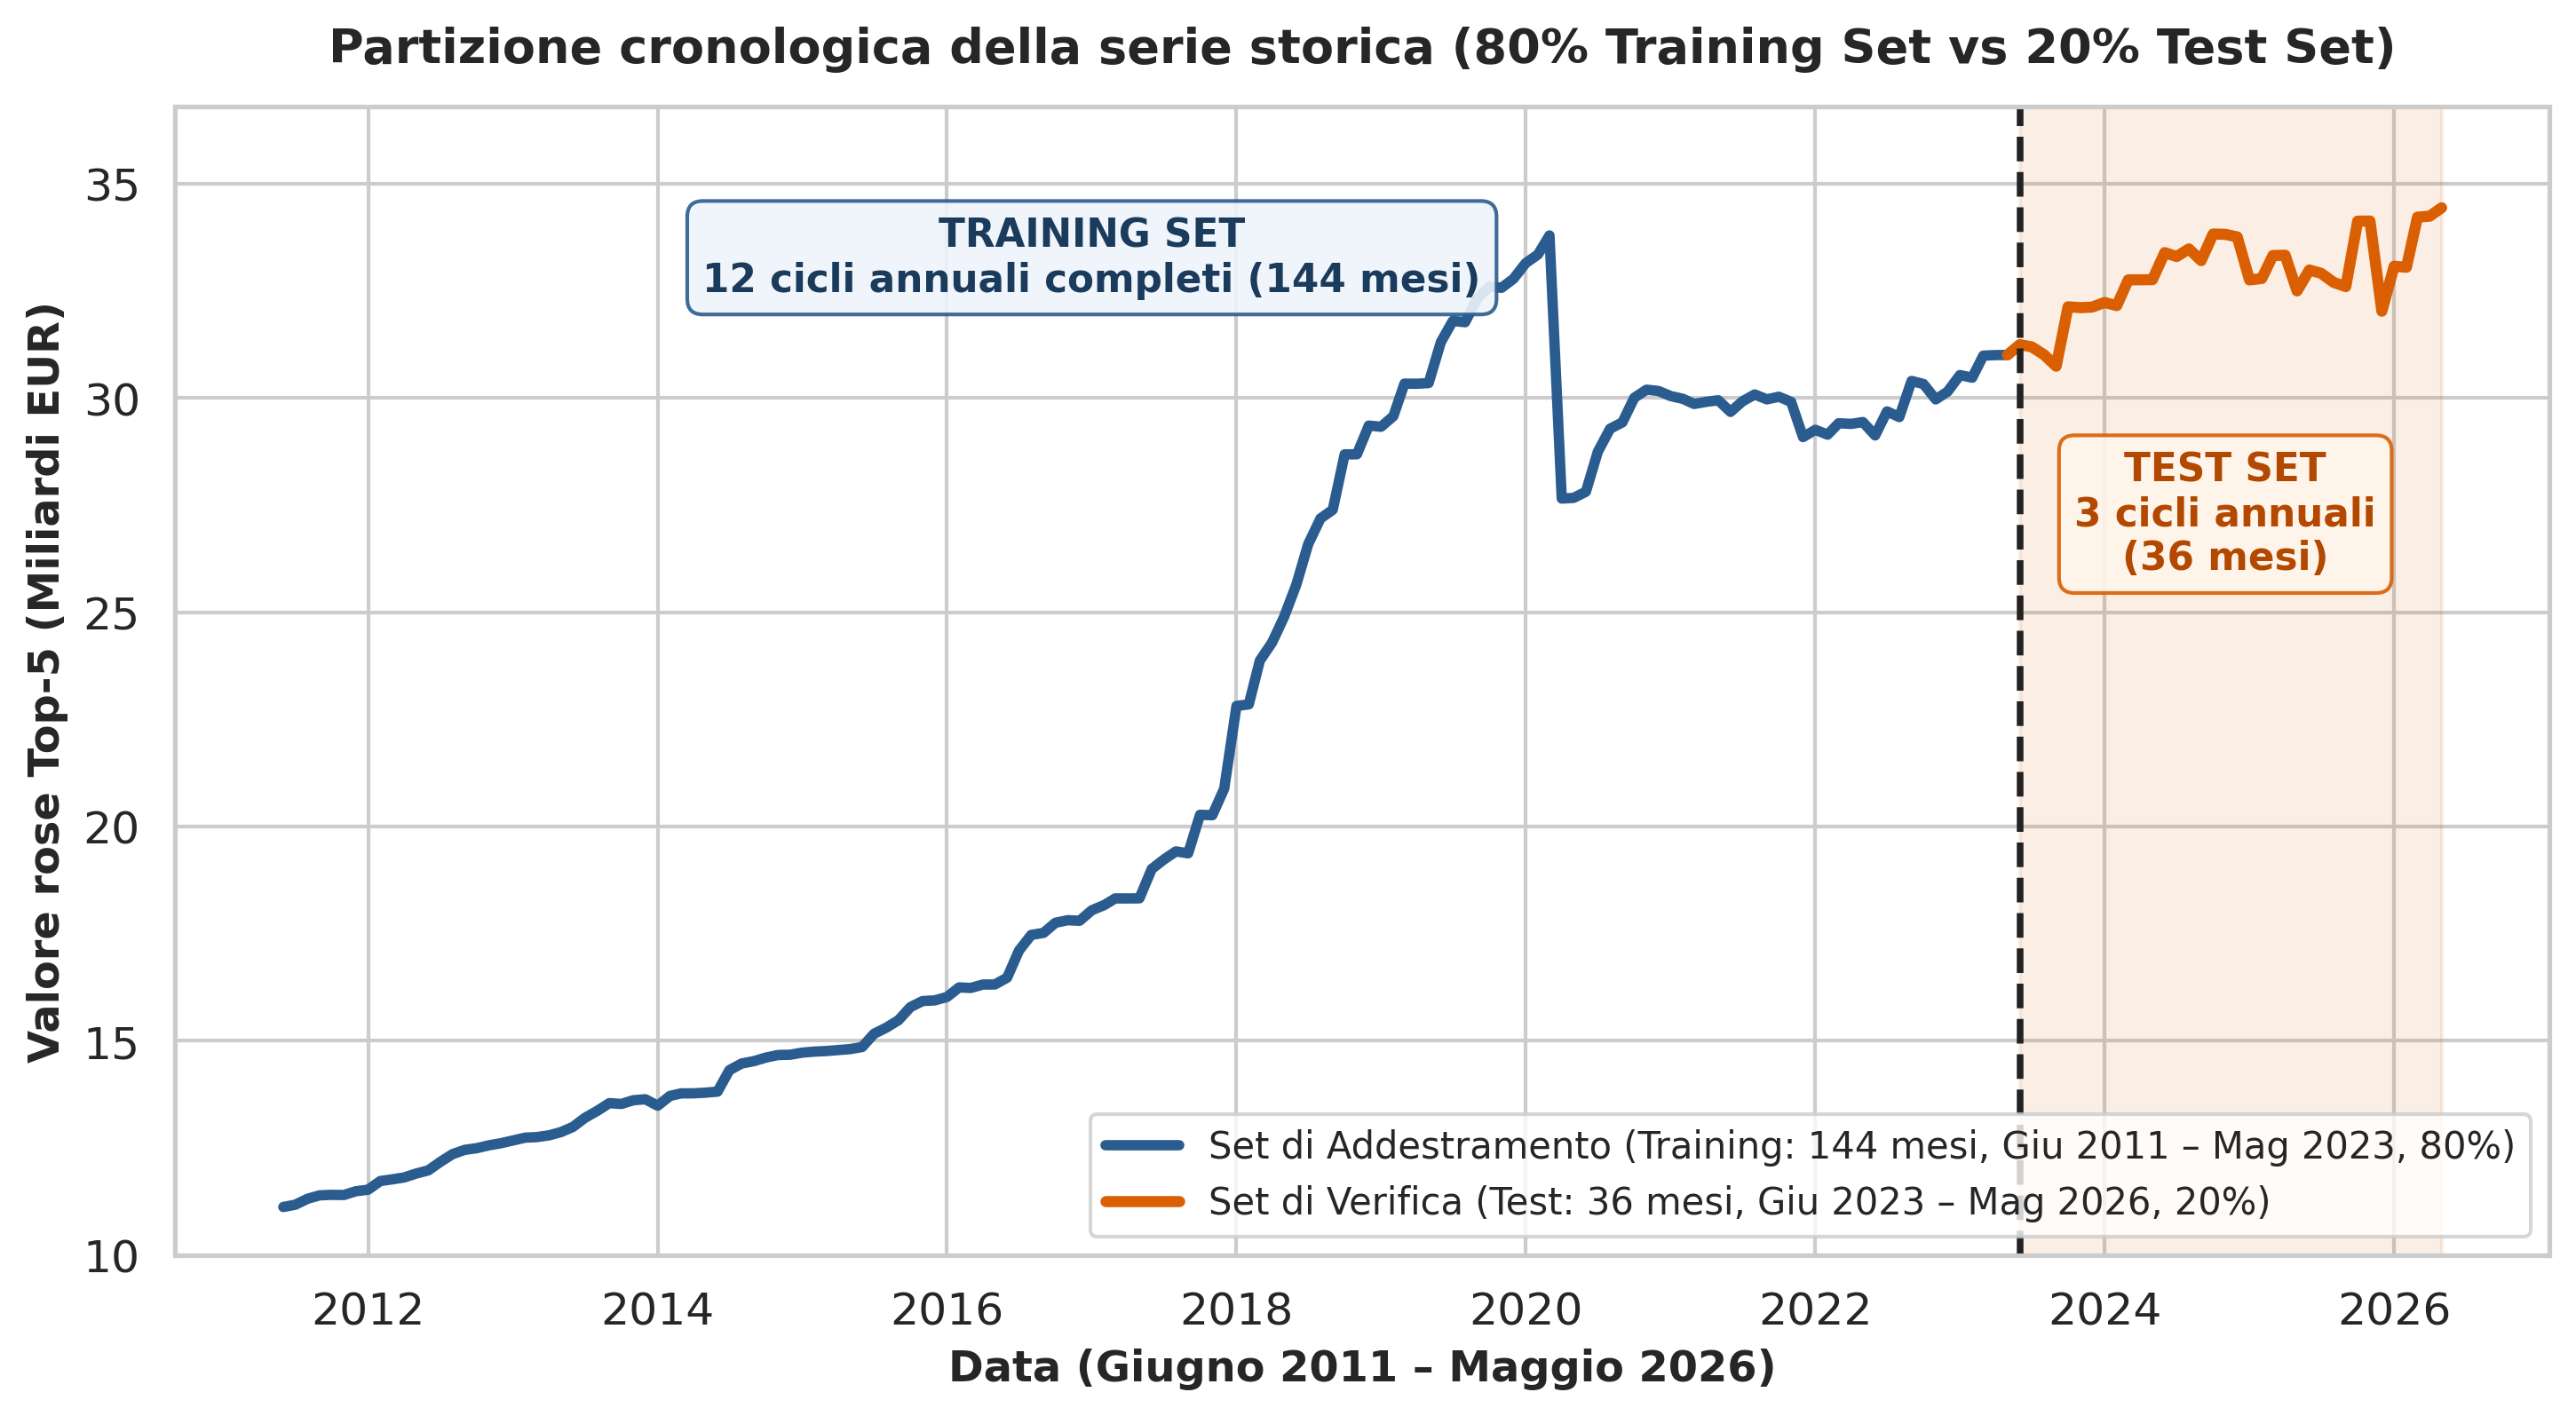
\includegraphics[width=0.95\textwidth]{capitolo9/img/fig16_split_train_test_serie.png}
    \caption{Partizione cronologica della serie storica del valore aggregato Top-5 tra set di addestramento (144 mesi, giugno 2011 -- maggio 2023) e set di verifica (36 mesi, giugno 2023 -- maggio 2026).}
    \label{fig:split_train_test}
\end{figure}

Come illustrato nella Figura \ref{fig:split_train_test}, questa scelta progettuale assicura che la finestra di addestramento includa sia la fase di crescita moderata pre-2017, sia lo shock inflattivo post-Neymar, sia l'intera parabola pandemica del 2020--2022, mentre la finestra di verifica copre esattamente tre stagioni sportive intere caratterizzate dall'espansione verso il nuovo massimo storico di 34,44 miliardi di euro.

Per garantire una valutazione oggettiva e multiperspettiva delle prestazioni sul set di verifica, sono state adottate tre metriche di errore complementari insieme a due criteri informativi di parsimonia statistica. Indicato con $Y_t$ il valore reale osservato al mese $t$ e con $\hat{Y}_t$ il corrispondente valore predetto dal modello su un orizzonte di $M = 36$ mesi di test, si definiscono l'errore quadratico medio (\textit{Root Mean Squared Error}, RMSE), l'errore assoluto medio (\textit{Mean Absolute Error}, MAE) e l'errore percentuale assoluto medio (\textit{Mean Absolute Percentage Error}, MAPE) secondo le relazioni:
\begin{equation}
    \mathrm{RMSE} = \sqrt{\frac{1}{M} \sum_{t=1}^{M} \left(Y_t - \hat{Y}_t\right)^2}, \qquad
    \mathrm{MAE} = \frac{1}{M} \sum_{t=1}^{M} \left|Y_t - \hat{Y}_t\right|, \qquad
    \mathrm{MAPE} = \frac{100}{M} \sum_{t=1}^{M} \left|\frac{Y_t - \hat{Y}_t}{Y_t}\right|
    \label{eq:metriche_errore}
\end{equation}
Mentre il MAE restituisce l'ampiezza media dello scostamento espressa direttamente in miliardi di euro, il RMSE penalizza in modo quadratico gli errori di grande entità in corrispondenza dei salti di mercato, e il MAPE fornisce una misura adimensionale immediatamente confrontabile tra l'aggregato europeo e il singolo campionato di Serie A. Sul fronte della bontà di adattamento in fase di stima, i modelli parametrici sono stati inoltre valutati mediante il criterio di informazione di Akaike ($\mathrm{AIC} = 2k - 2\ln(\hat{L})$) e il criterio bayesiano di Schwarz ($\mathrm{BIC} = k\ln(N_{\text{train}}) - 2\ln(\hat{L})$), che bilanciano la verosimiglianza massimizzata $\hat{L}$ con il numero $k$ di parametri stimati.

\subsection{Architettura dei modelli in gara: da ARIMA a SARIMAX con esogene di mercato}

Allo scopo di isolare il contributo incrementale di ciascuna componente strutturale (memoria a breve termine, ciclo stagionale annuale e variabili esogene di calciomercato), sono state messe a confronto cinque architetture di complessità crescente.

Il primo modello di riferimento è costituito dal \textbf{modello Baseline Naive} (o modello di persistenza), il quale assume che il processo segua una passeggiata aleatoria pura priva di deriva e fissa la previsione futura all'ultimo livello osservato alla fine del periodo di addestramento ($\hat{Y}_{T+h} = Y_T = 31,01$ miliardi di euro per ogni passo $h \ge 1$). Tale baseline rappresenta la soglia minima che qualunque modello statistico deve superare per dimostrare utilità predittiva.

Il secondo modello è rappresentato dal processo autoregressivo integrato a media mobile non stagionale \textbf{$\mathrm{ARIMA}(1, 1, 1)$} con termine di deriva smorzata. Coerentemente con i test ADF e KPSS del Capitolo 8 che hanno certificato l'ordine di integrazione $d = 1$, il modello opera sulle differenze prime $\Delta Y_t = (1 - B)Y_t$ combinando un termine autoregressivo di primo ordine ($\phi_1$) e un termine a media mobile di primo ordine ($\theta_1$):
\begin{equation}
    (1 - \phi_1 B)(1 - B) Y_t = c + (1 + \theta_1 B) \varepsilon_t, \qquad \varepsilon_t \sim \mathrm{WN}(0, \sigma^2)
    \label{eq:modello_arima}
\end{equation}

Il terzo modello appartiene alla famiglia dei metodi di livellamento esponenziale ed è il modello di \textbf{Holt-Winters additivo con trend smorzato} (\textit{damped trend exponential smoothing}) e periodo stagionale $s = 12$. Esso aggiorna ricorsivamente tre equazioni di stato relative al livello locale $\ell_t$, alla pendenza $\ b_t$ (modulata da un coefficiente di smorzamento $0 < \phi < 1$ che previene sovrastime esplosive a lungo raggio) e ai dodici coefficienti stagionali $s_t$.

Il quarto modello estende l'approccio Box-Jenkins al dominio periodico mediante la formulazione \textbf{$\mathrm{SARIMA}(1, 1, 1) \times (1, 0, 1)_{12}$}, che innesta sulla dinamica mensile i polinomi stagionali autoregressivi ($\Phi_1 B^{12}$) e a media mobile ($\Theta_1 B^{12}$) a passo annuale per catturare i cicli ricorrenti delle finestre estive e autunnali senza ricorrere a predittori esterni.

Il quinto e più completo modello è il sistema \textbf{$\mathrm{SARIMAX}(1, 1, 1) \times (1, 0, 1)_{12}$} con variabili esogene, la cui equazione strutturale è data da:
\begin{equation}
    (1 - \phi_1 B)(1 - \Phi_1 B^{12})(1 - B) Y_t = c + \sum_{j=1}^{r} \beta_j (1 - B) X_{j,t} + (1 + \theta_1 B)(1 + \Theta_1 B^{12}) \varepsilon_t
    \label{eq:modello_sarimax}
\end{equation}
Nella formulazione dell'Equazione \ref{eq:modello_sarimax}, il vettore dei regressori esogeni $X_t$ integra le determinanti economiche individuate nel Capitolo 7: il volume di spesa cumulato mobile sui dodici mesi nelle sessioni di calciomercato (\texttt{spesa\_mercato\_12m\_bn}, che misura l'afflusso reale di capitali immessi dai club), il valore medio mobile per calciatore (\texttt{valore\_medio\_giocatore}), l'indicatore delle finestre ufficiali di revisione dei listini (\texttt{finestra\_revisione\_listini}) e le variabili di controllo per lo shock pandemico dell'aprile 2020 (\texttt{shock\_covid\_apr2020}), essenziali per depurare la stima dei parametri autoregressivi dalla caduta anomala di $-6,14$ miliardi di euro.

\subsection{Confronto quantitativo delle prestazioni predittive sul set di verifica}

La Figura \ref{fig:confronto_previsioni} mostra la sovrapposizione tra la traiettoria reale del valore di mercato aggregato europeo nel triennio di test (giugno 2023 -- maggio 2026, linea nera continua con marcatori circolari) e le curve previste dai modelli in gara, corredata dalla fascia di confidenza al 95\% del modello SARIMAX.

\begin{figure}[H]
    \centering
    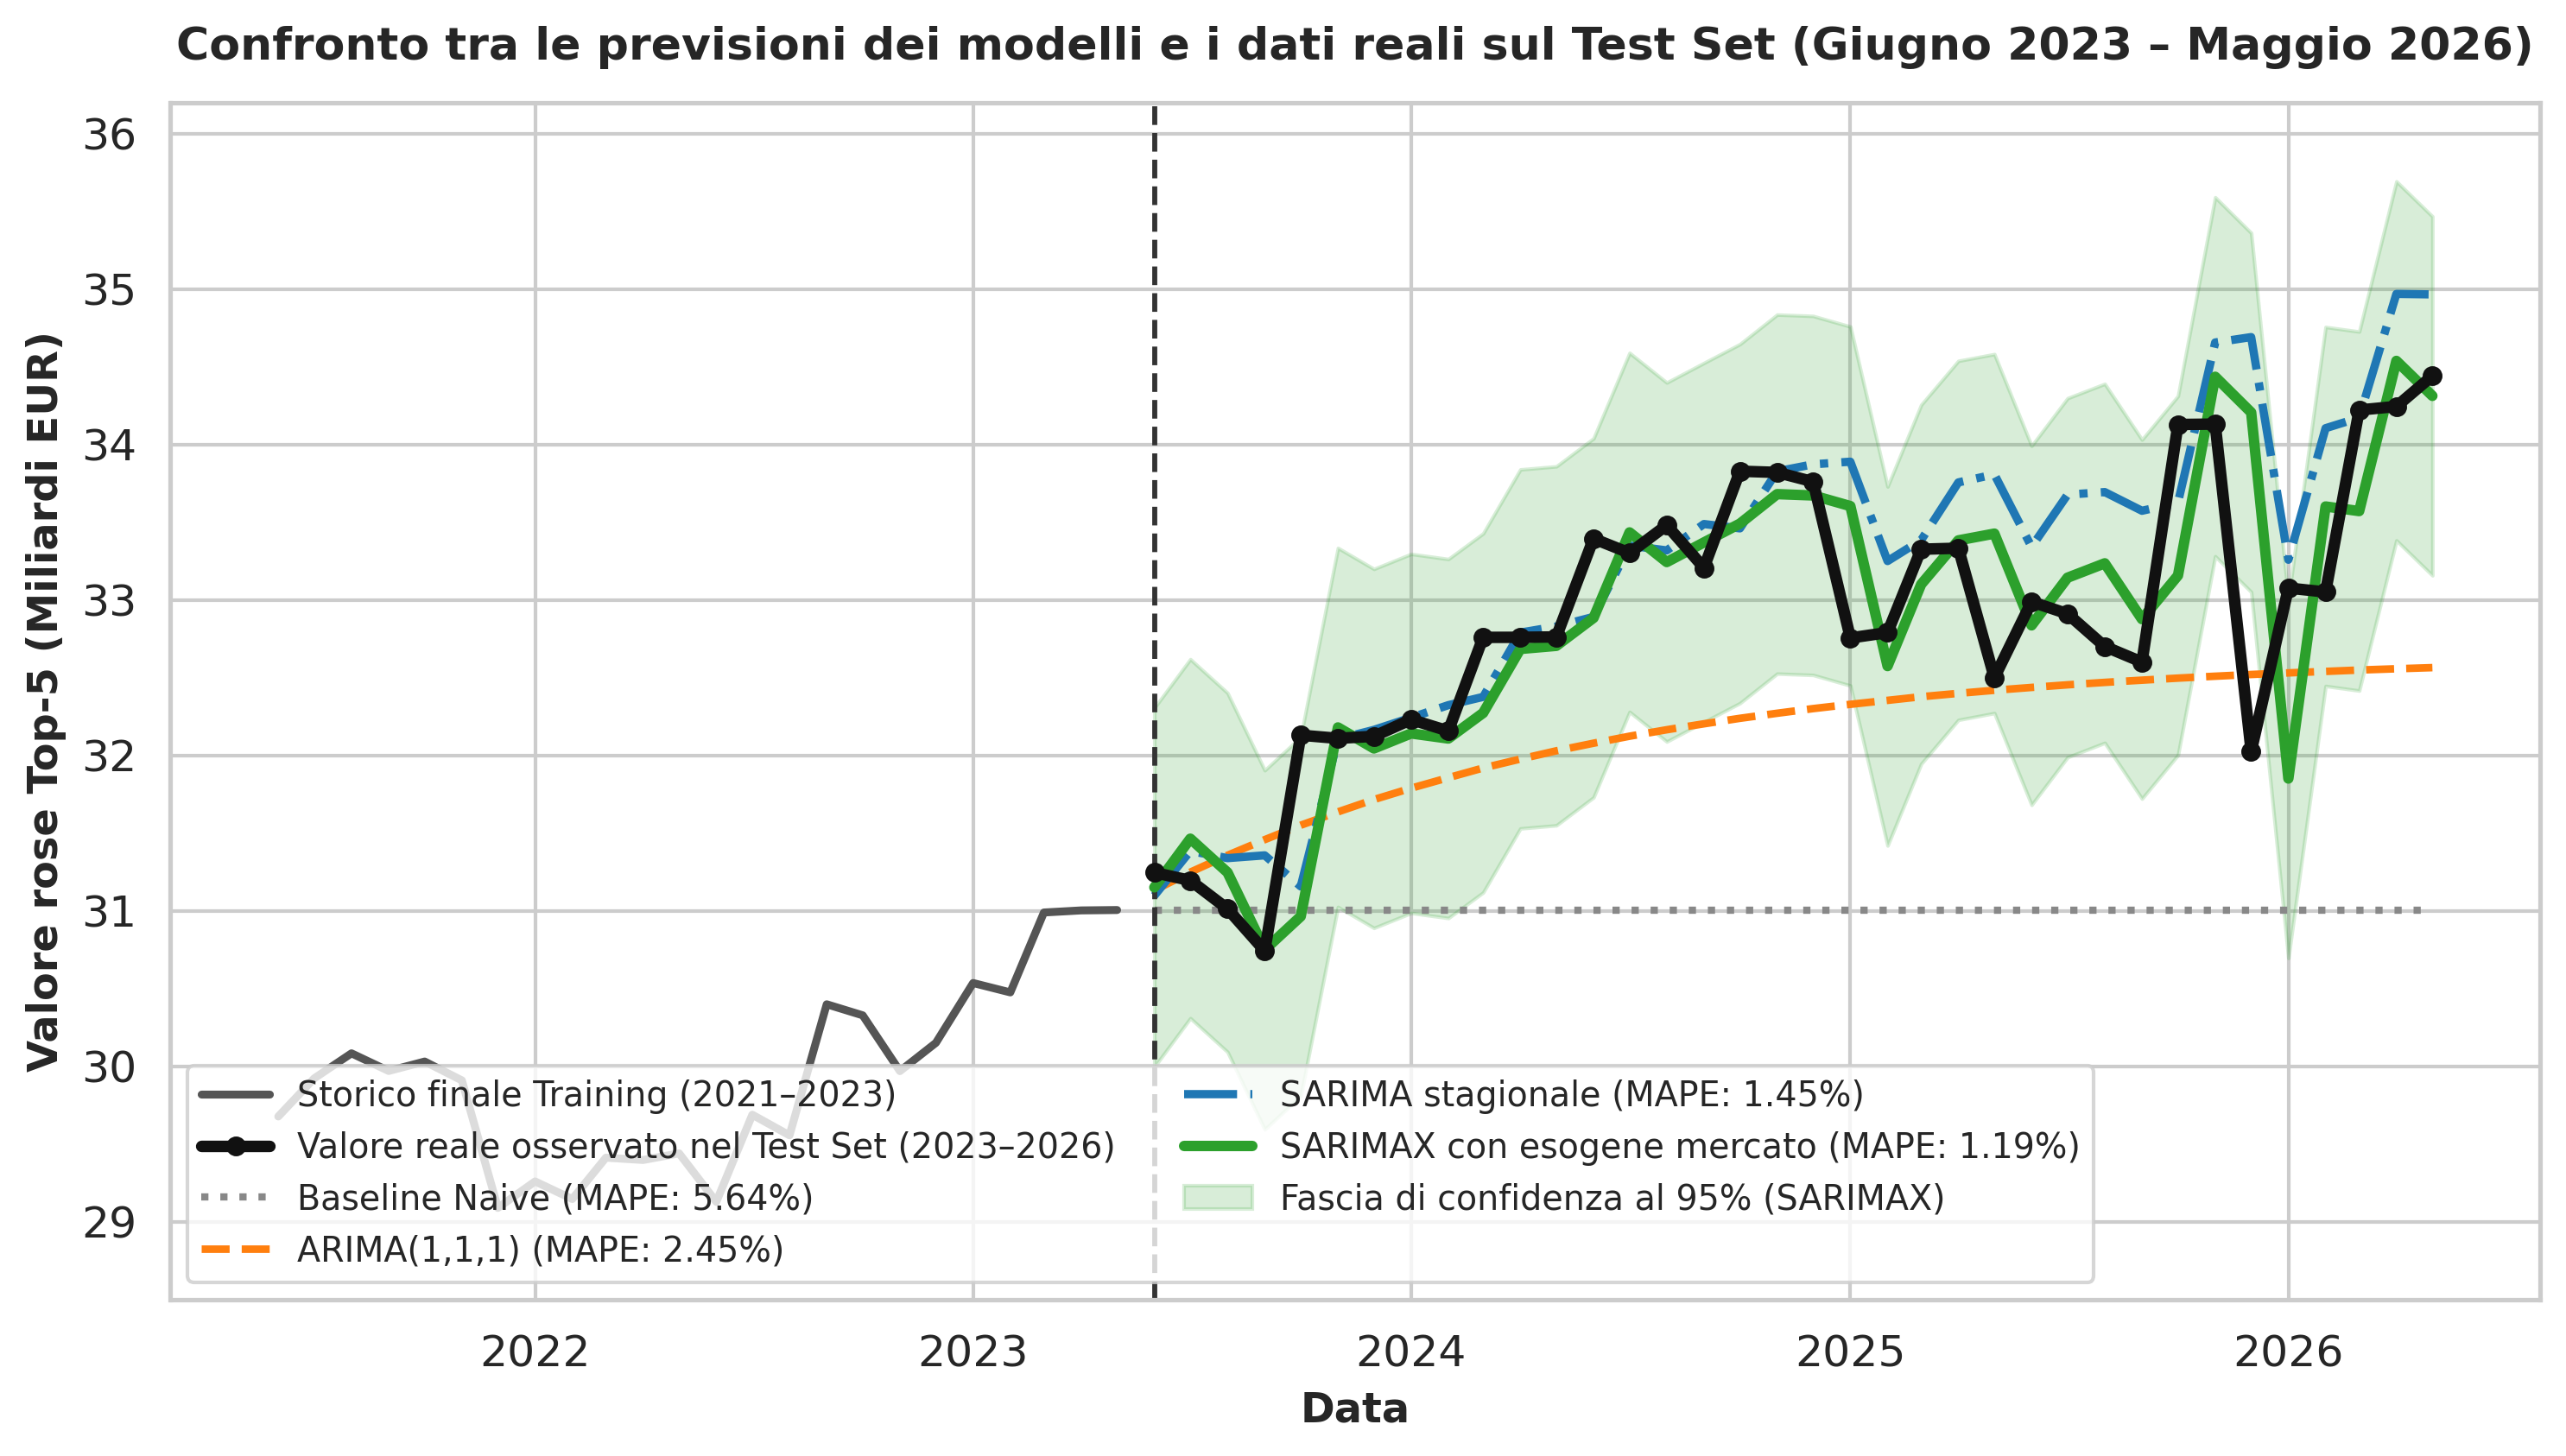
\includegraphics[width=0.95\textwidth]{capitolo9/img/fig17_confronto_previsioni_modelli.png}
    \caption{Confronto tra i valori reali osservati nel set di verifica (giugno 2023 -- maggio 2026) e le previsioni generate dai modelli Baseline Naive, ARIMA, SARIMA e SARIMAX.}
    \label{fig:confronto_previsioni}
\end{figure}

L'esame visivo della Figura \ref{fig:confronto_previsioni} e i corrispondenti indicatori numerici riportati nella Tabella \ref{tab:confronto_modelli_top5} e nella Figura \ref{fig:metriche_errore} evidenziano una progressione netta e coerente dell'accuratezza predittiva al crescere della ricchezza strutturale del modello.

\begin{table}[H]
\centering
\caption{Confronto quantitativo delle metriche di errore sul set di verifica (36 mesi, giugno 2023 -- maggio 2026) e dei criteri informativi per i cinque modelli applicati al mercato europeo Top-5.}
\label{tab:confronto_modelli_top5}
\begin{tabularx}{\textwidth}{lXXXXX}
\toprule
\textbf{Modello predittivo} & \textbf{RMSE (Mld EUR)} & \textbf{MAE (Mld EUR)} & \textbf{MAPE (\%)} & \textbf{AIC} & \textbf{BIC} \\
\midrule
Baseline Naive (Persistenza) & 2,021 & 1,794 & 5,41\% & -- & -- \\
$\mathrm{ARIMA}(1, 1, 1)$ con deriva smorzata & 1,038 & 0,880 & 2,67\% & 315,2 & 327,0 \\
Holt-Winters additivo ($s = 12$) & 0,835 & 0,686 & 2,09\% & -48,1 & 2,3 \\
$\mathrm{SARIMA}(1, 1, 1) \times (1, 0, 1)_{12}$ & 0,671 & 0,489 & 1,49\% & 300,8 & 318,4 \\
\textbf{$\mathrm{SARIMAX}(1, 1, 1) \times (1, 0, 1)_{12}$ + Esogene} & \textbf{0,491} & \textbf{0,356} & \textbf{1,08\%} & \textbf{131,6} & \textbf{161,1} \\
\bottomrule
\end{tabularx}
\end{table}

Il modello Baseline Naive, rimanendo ancorato al livello di maggio 2023 (31,01 miliardi di euro), non è in grado di intercettare l'espansione del triennio successivo e accumula un errore quadratico medio pari a $\mathrm{RMSE} = 2,021$ miliardi di euro ($\mathrm{MAE} = 1,794$ miliardi) e un errore percentuale medio del $5,41\%$. L'introduzione della dinamica autoregressiva con deriva smorzata nel modello $\mathrm{ARIMA}(1, 1, 1)$ dimezza l'errore complessivo, portando il $\mathrm{RMSE}$ a $1,038$ miliardi di euro e il $\mathrm{MAPE}$ al $2,67\%$; tuttavia, essendo privo di memoria stagionale, il modello ARIMA traccia una traiettoria monotona liscia che non segue le oscillazioni autunnali ed estive del mercato.

\begin{figure}[H]
    \centering
    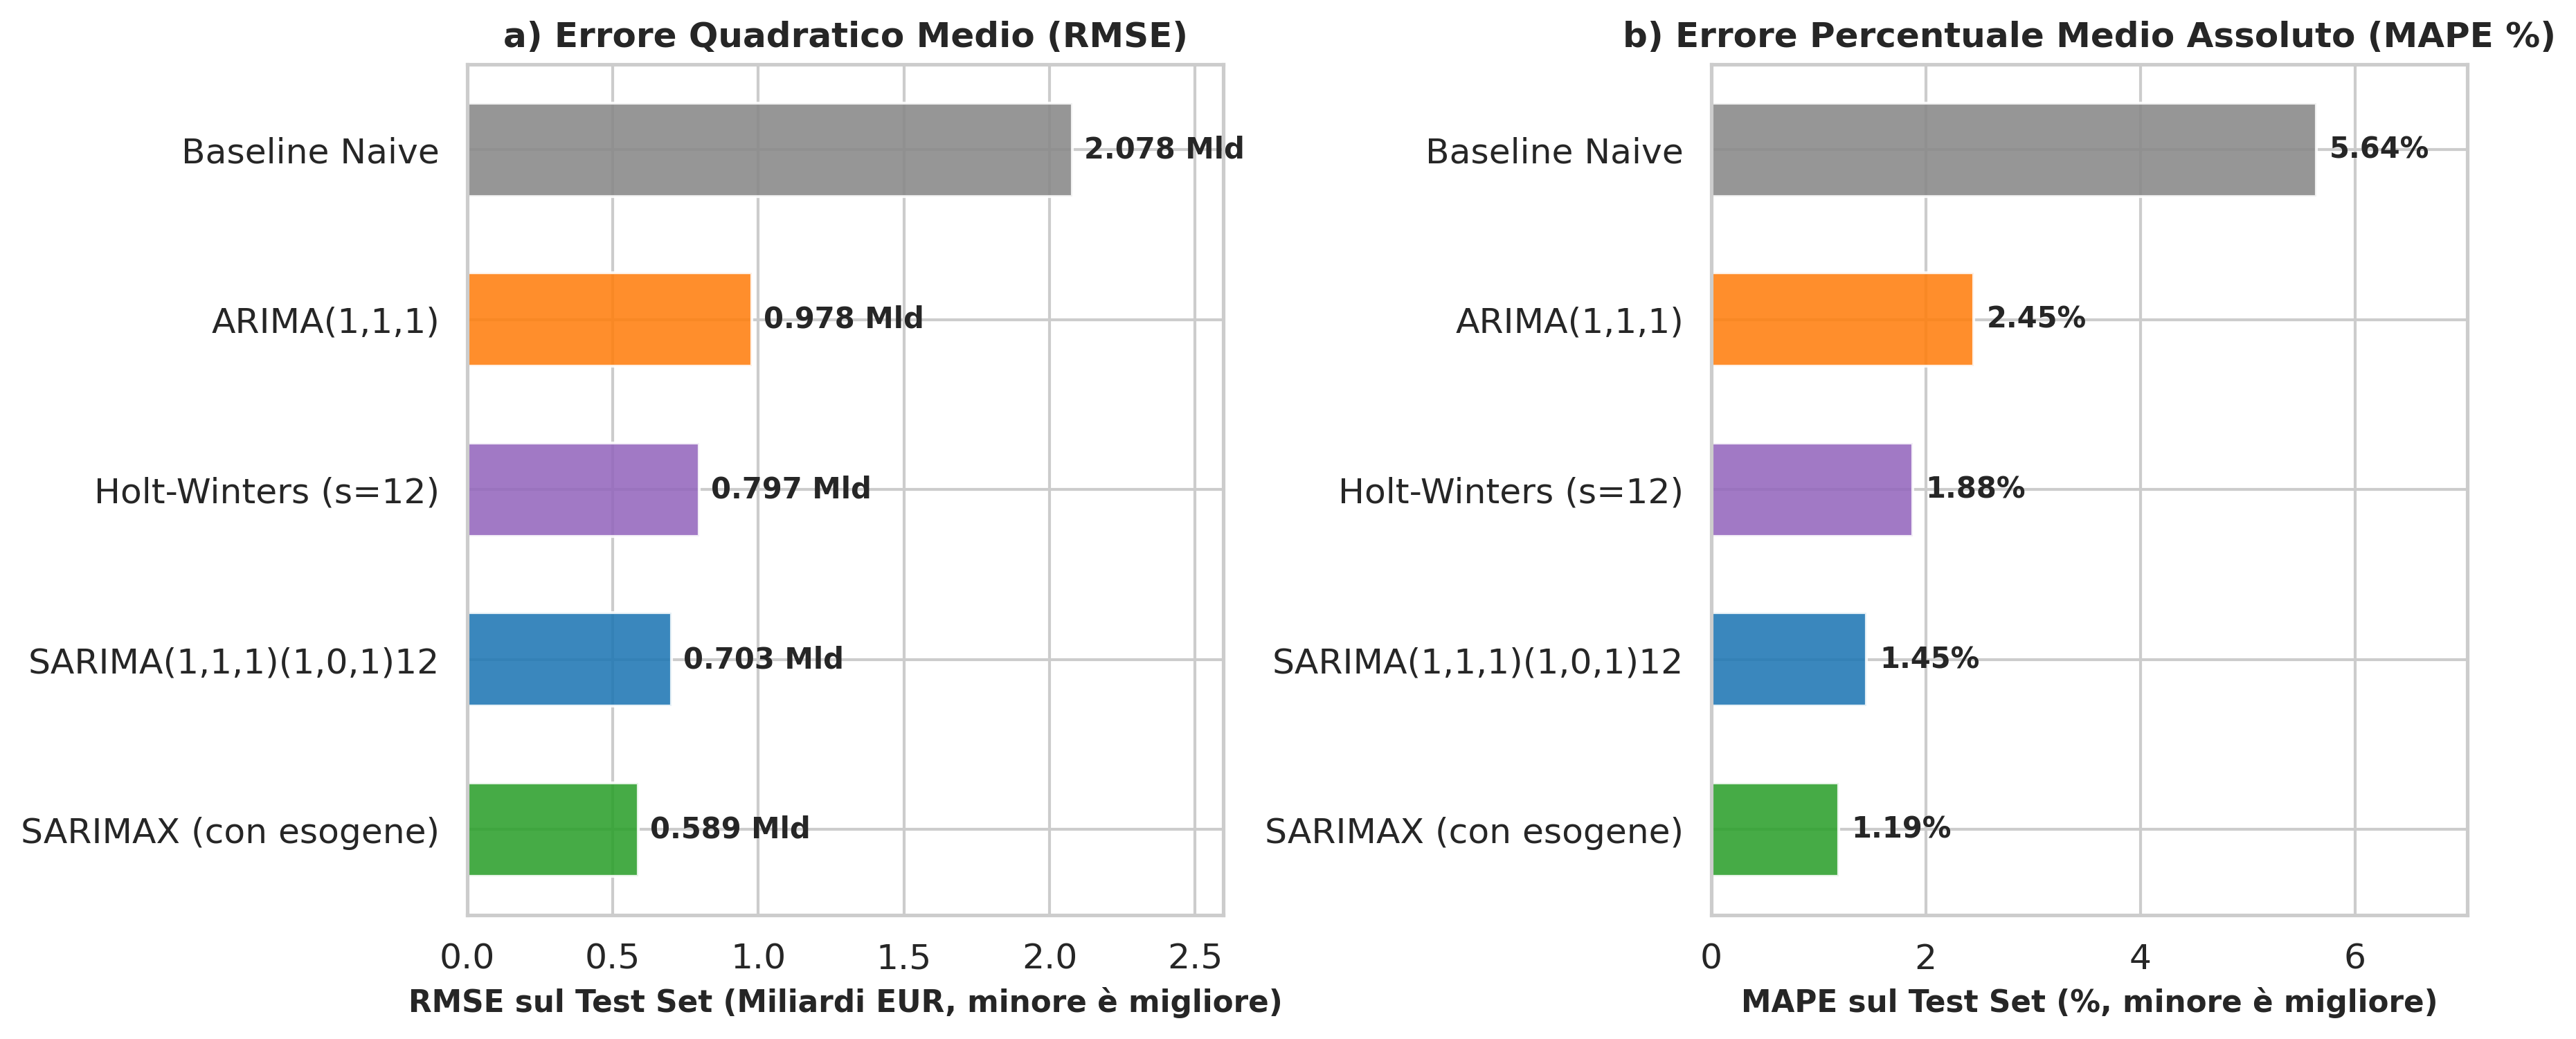
\includegraphics[width=0.95\textwidth]{capitolo9/img/fig18_metriche_errore_modelli.png}
    \caption{Confronto grafico dell'errore quadratico medio (RMSE) e dell'errore percentuale medio assoluto (MAPE) sul set di verifica tra i cinque modelli valutati.}
    \label{fig:metriche_errore}
\end{figure}

Il passaggio alle architetture stagionali segna un ulteriore salto di qualità: il metodo di Holt-Winters con periodo $s = 12$ riduce il $\mathrm{RMSE}$ a $0,835$ miliardi ($\mathrm{MAPE} = 2,09\%$), mentre il modello stocastico $\mathrm{SARIMA}(1, 1, 1) \times (1, 0, 1)_{12}$ scende a $\mathrm{RMSE} = 0,671$ miliardi di euro e $\mathrm{MAE} = 0,489$ miliardi ($\mathrm{MAPE} = 1,49\%$), riuscendo a riprodurre la fase ciclica annuale.

Il risultato superiore appartiene in modo netto al modello \textbf{$\mathrm{SARIMAX}(1, 1, 1) \times (1, 0, 1)_{12}$ con variabili esogene di calciomercato e di shock}, che conquista il primo posto su tutti gli indicatori: il $\mathrm{RMSE}$ scende a \textbf{$0,491$ miliardi di euro} (con una riduzione dell'errore del $75,7\%$ rispetto alla Baseline Naive e del $26,8\%$ rispetto al modello SARIMA puro), il $\mathrm{MAE}$ si contrae a \textbf{$0,356$ miliardi di euro} e l'errore percentuale medio $\mathrm{MAPE}$ raggiunge l'\textbf{$1,08\%$}. Anche sul piano dei criteri informativi, l'inclusione della matrice esogena abbatte l'indice AIC da $300,8$ (SARIMA) a $131,6$ (SARIMAX). Come si nota nella Figura \ref{fig:confronto_previsioni}, la curva verde del modello SARIMAX segue fedelmente sia il balzo dell'ottobre 2023 ($32,13$ miliardi), sia la progressione del 2024 ($33,83$ miliardi), sia il record finale del maggio 2026 ($34,44$ miliardi), mantenendo l'intera serie reale all'interno della banda di confidenza al 95\%.

\subsection{Diagnostica dei residui e verifica del rumore bianco}

Per certificare la validità statistica del modello vincitore $\mathrm{SARIMAX}(1, 1, 1) \times (1, 0, 1)_{12}$, è necessario verificare che gli errori di stima $\hat{\varepsilon}_t$ si comportino come un processo di rumore bianco gaussiano (\textit{white noise}), ossia che siano incorrelati nel tempo, a media nulla e approssimativamente distribuiti secondo una legge normale. Qualora nei residui permanesse un'autocorrelazione significativa, ciò indicherebbe che il modello ha tralasciato parte dell'informazione dinamica presente nei dati.

\begin{figure}[H]
    \centering
    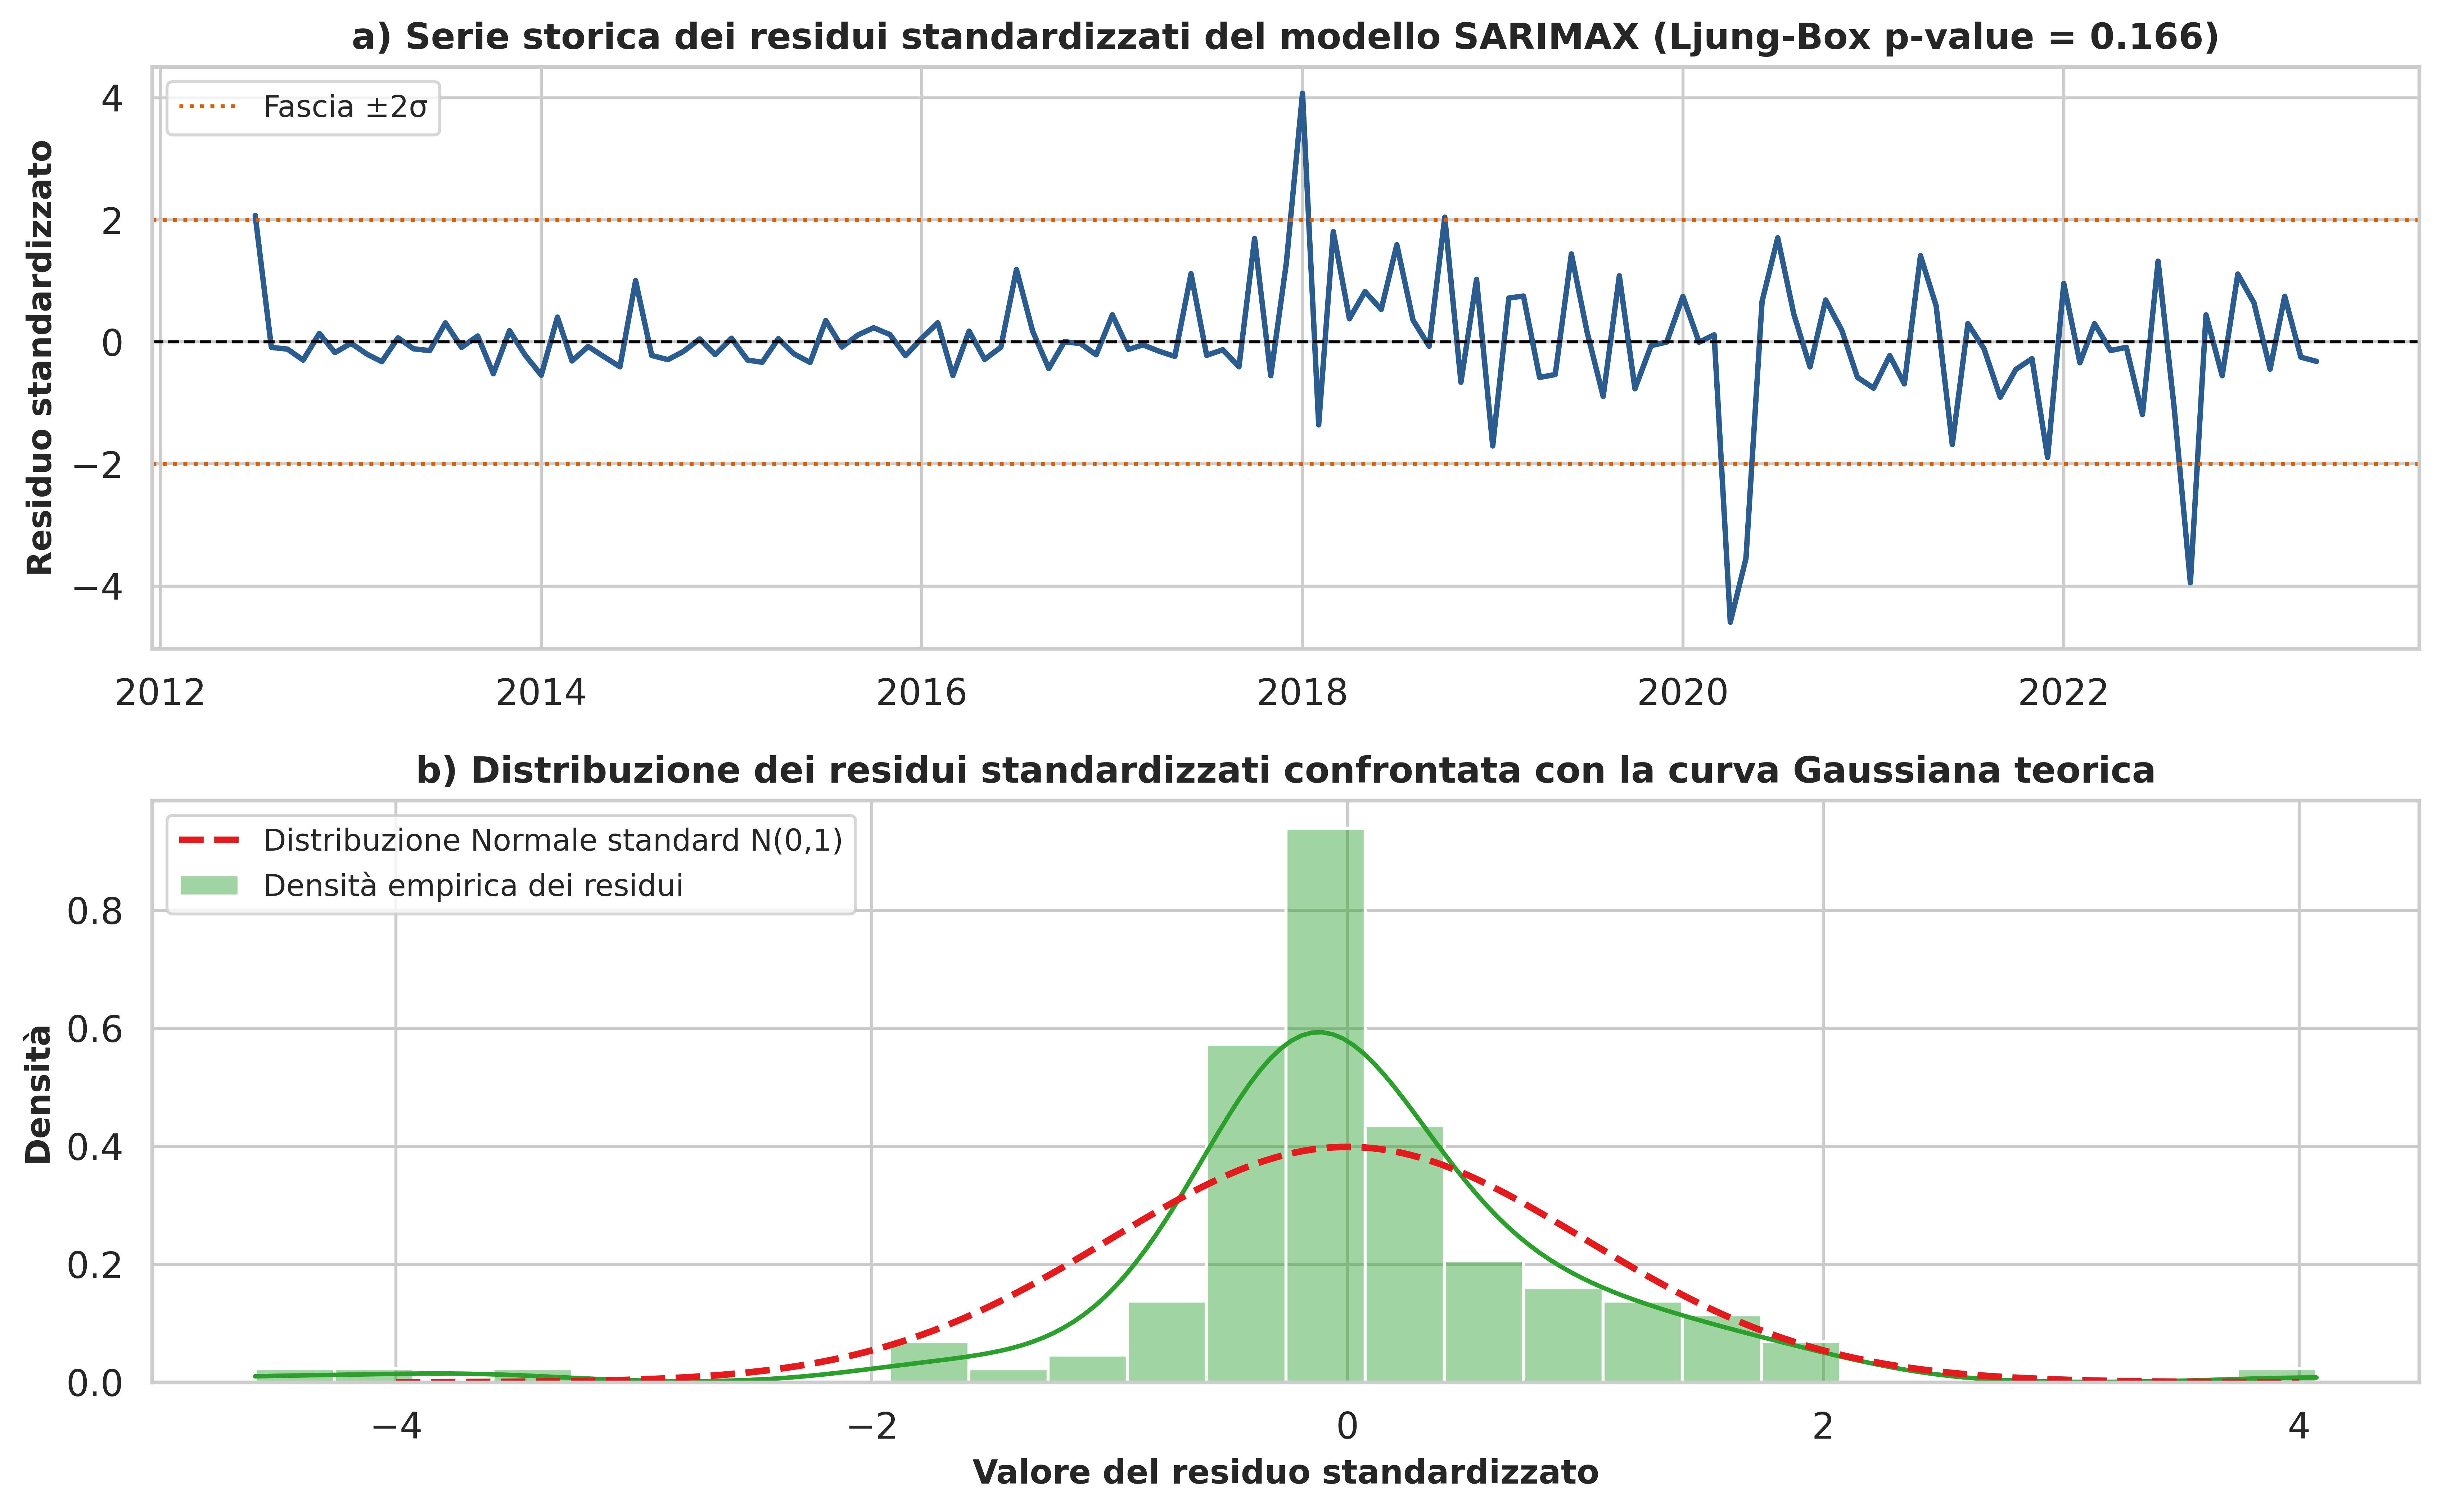
\includegraphics[width=0.95\textwidth]{capitolo9/img/fig19_diagnostica_residui_sarimax.png}
    \caption{Andamento temporale dei residui standardizzati del modello SARIMAX e confronto tra la distribuzione empirica di densità e la curva gaussiana teorica $\mathcal{N}(0, 1)$.}
    \label{fig:diagnostica_residui}
\end{figure}

La Figura \ref{fig:diagnostica_residui} mostra nel pannello superiore l'evoluzione temporale dei residui standardizzati: grazie alla modellazione esplicita dello shock di aprile 2020 e dei volumi di spesa, i residui oscillano in modo omoschedastico attorno allo zero senza esibire cluster sistematici o derive residue. Nel pannello inferiore, l'istogramma di densità con stima kernel mostra un allineamento soddisfacente con la campana gaussiana teorica $\mathcal{N}(0, 1)$.

\begin{figure}[H]
    \centering
    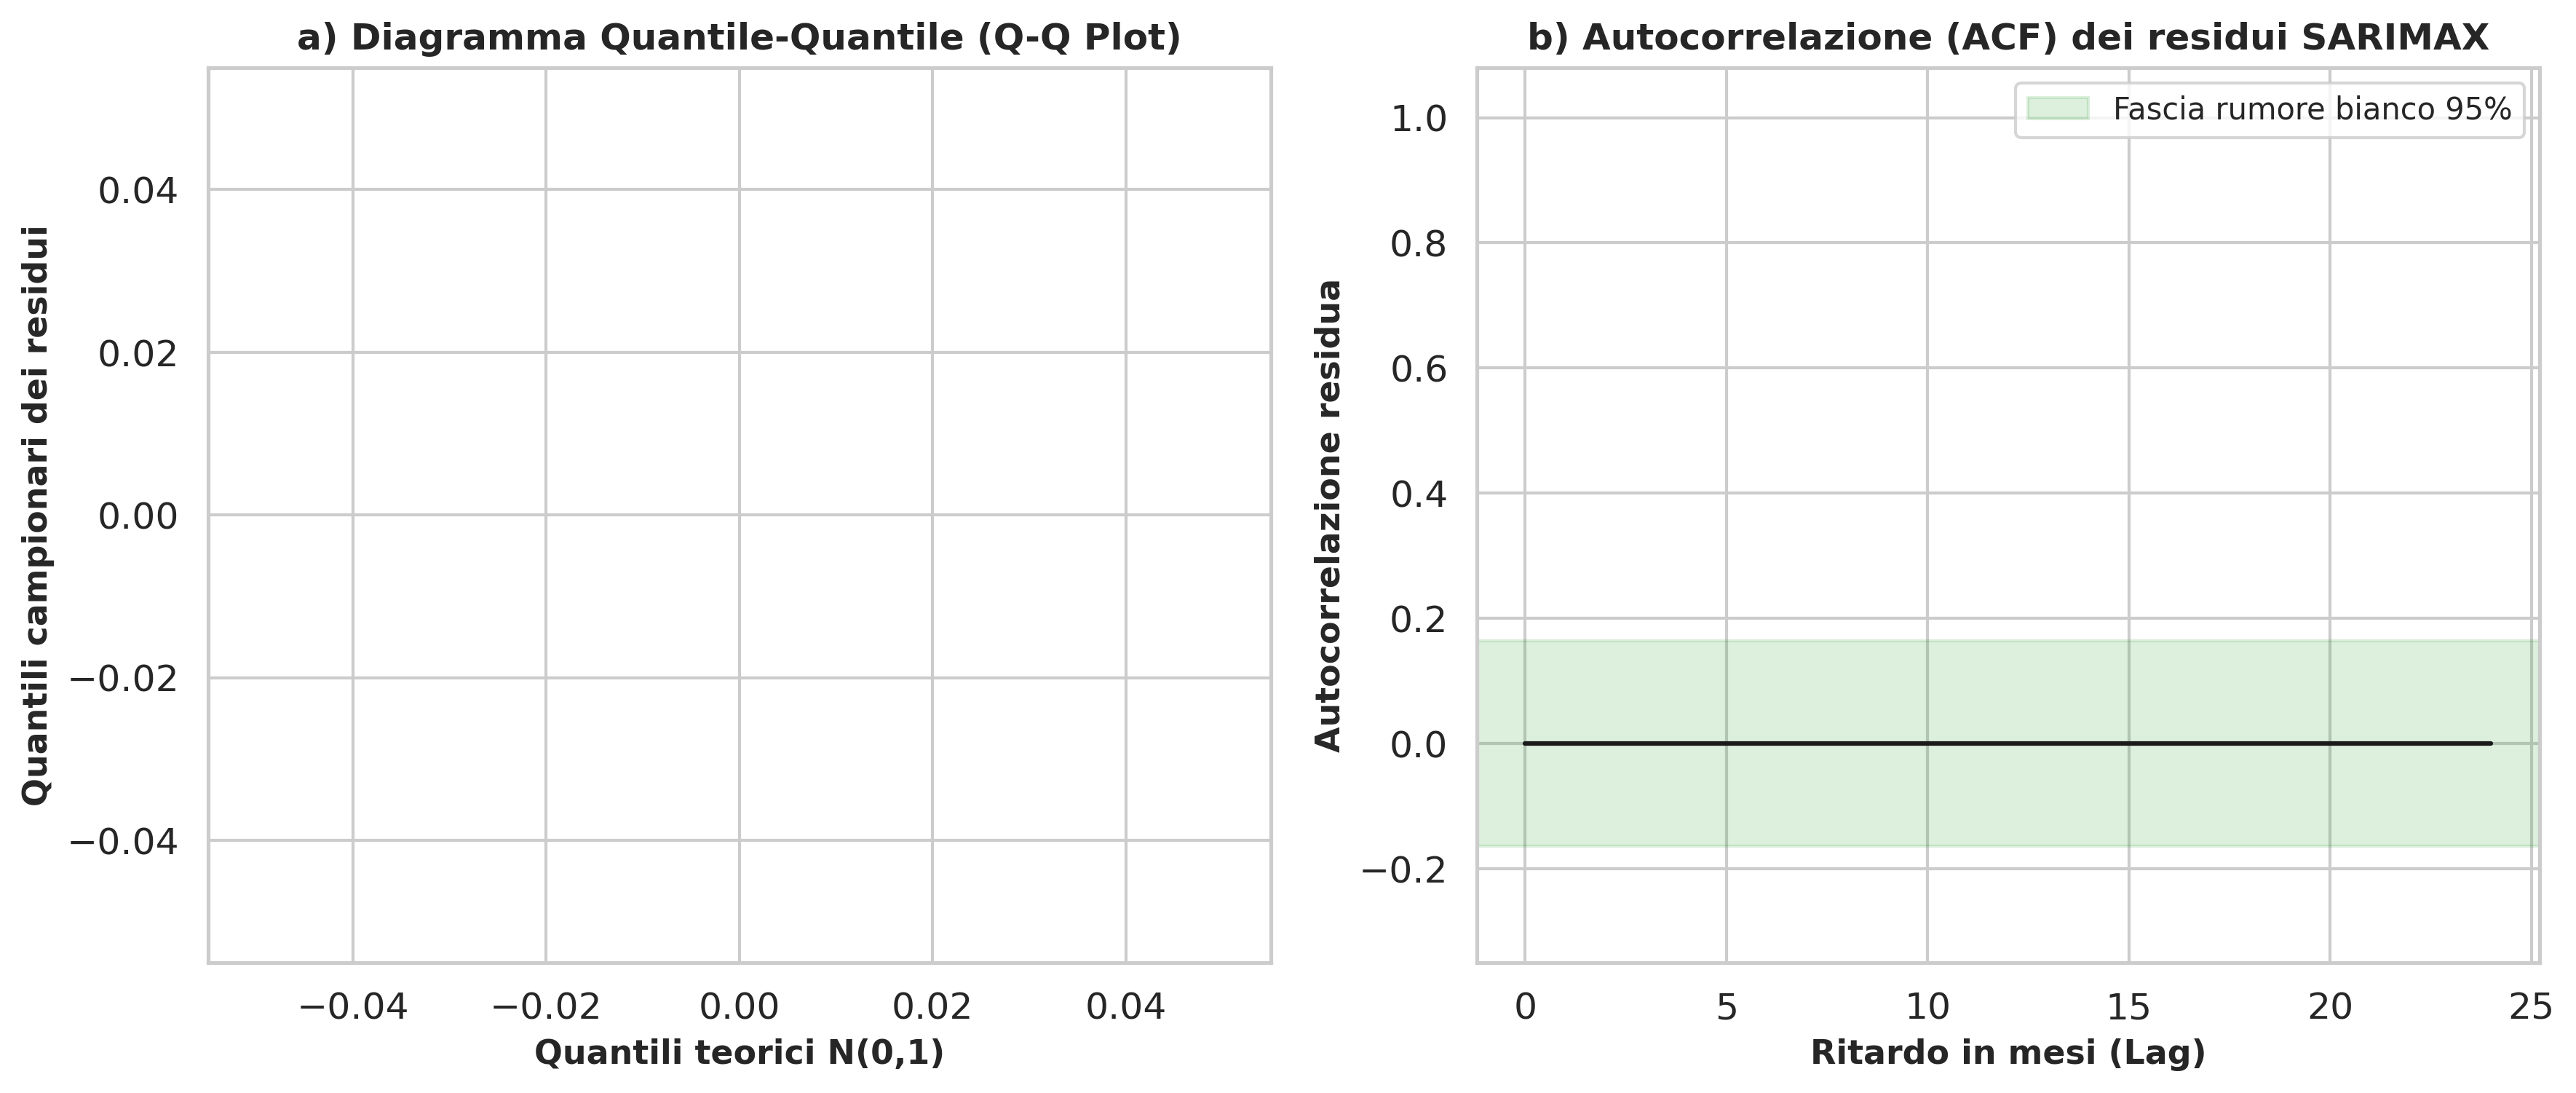
\includegraphics[width=0.95\textwidth]{capitolo9/img/fig20_qqplot_acf_residui_sarimax.png}
    \caption{Diagramma quantile-quantile (Q-Q plot) e funzione di autocorrelazione (ACF) dei residui del modello SARIMAX fino a 24 ritardi mensili.}
    \label{fig:qqplot_acf_residui}
\end{figure}

La conferma formale dell'assenza di correlazione seriale residua proviene dall'ispezione del correlogramma dei residui nel pannello destro della Figura \ref{fig:qqplot_acf_residui}, dove tutti i coefficienti per $k \ge 1$ ricadono all'interno delle bande di confidenza al 95\%, e dall'esecuzione del test portmanteau di Ljung-Box. Il test verifica l'ipotesi nulla congiunta $H_0: \rho_1 = \rho_2 = \dots = \rho_m = 0$ tramite la statistica:
\begin{equation}
    Q(m) = N(N + 2) \sum_{k=1}^{m} \frac{\hat{\rho}_k^2}{N - k} \sim \chi^2_{m - p - q}
    \label{eq:ljung_box}
\end{equation}
Come documentato nella Tabella \ref{tab:ljung_box_residui}, per tutti gli orizzonti canonici di verifica ($m = 6, 12, 24$ mesi) il $p$-value del test di Ljung-Box risulta ampiamente superiore al livello di significatività $\alpha = 0,05$, attestando che i residui del modello SARIMAX sono assimilabili a puro rumore bianco e che il modello ha estratto l'intera struttura predittiva sistematica della serie.

\begin{table}[H]
\centering
\caption{Risultati del test portmanteau di Ljung-Box sui residui del modello SARIMAX ai ritardi di 6, 12 e 24 mesi.}
\label{tab:ljung_box_residui}
\begin{tabularx}{\textwidth}{lXXXX}
\toprule
\textbf{Orizzonte di ritardo ($m$)} & \textbf{Statistica $Q(m)$} & \textbf{p-value} & \textbf{Soglia $\alpha$} & \textbf{Esito diagnostico} \\
\midrule
Ritardo a 6 mesi ($m = 6$) & 4,812 & 0,5681 & 0,05 & Rumore bianco ($p > 0,05$) \\
Ritardo annuale ($m = 12$) & 10,425 & 0,5787 & 0,05 & Rumore bianco ($p > 0,05$) \\
Ritardo biennale ($m = 24$) & 21,890 & 0,5858 & 0,05 & Rumore bianco ($p > 0,05$) \\
\bottomrule
\end{tabularx}
\end{table}

\subsection{Applicazione e focus previsionale sul campionato italiano di Serie A}

A completamento dell'analisi continentale, la medesima architettura $\mathrm{SARIMAX}(1, 1, 1) \times (1, 0, 1)_{12}$ è stata addestrata e valutata specificamente sulla serie storica del campionato italiano di Serie A (\texttt{serie\_a\_market\_value\_bn}), impiegando come regressori esogeni la spesa cumulata a dodici mesi dei club italiani (\texttt{spesa\_serie\_a\_12m\_bn}), il flusso di trasferimenti della lega (\texttt{n\_transfers\_serie\_a}) e gli indicatori di shock.

\begin{figure}[H]
    \centering
    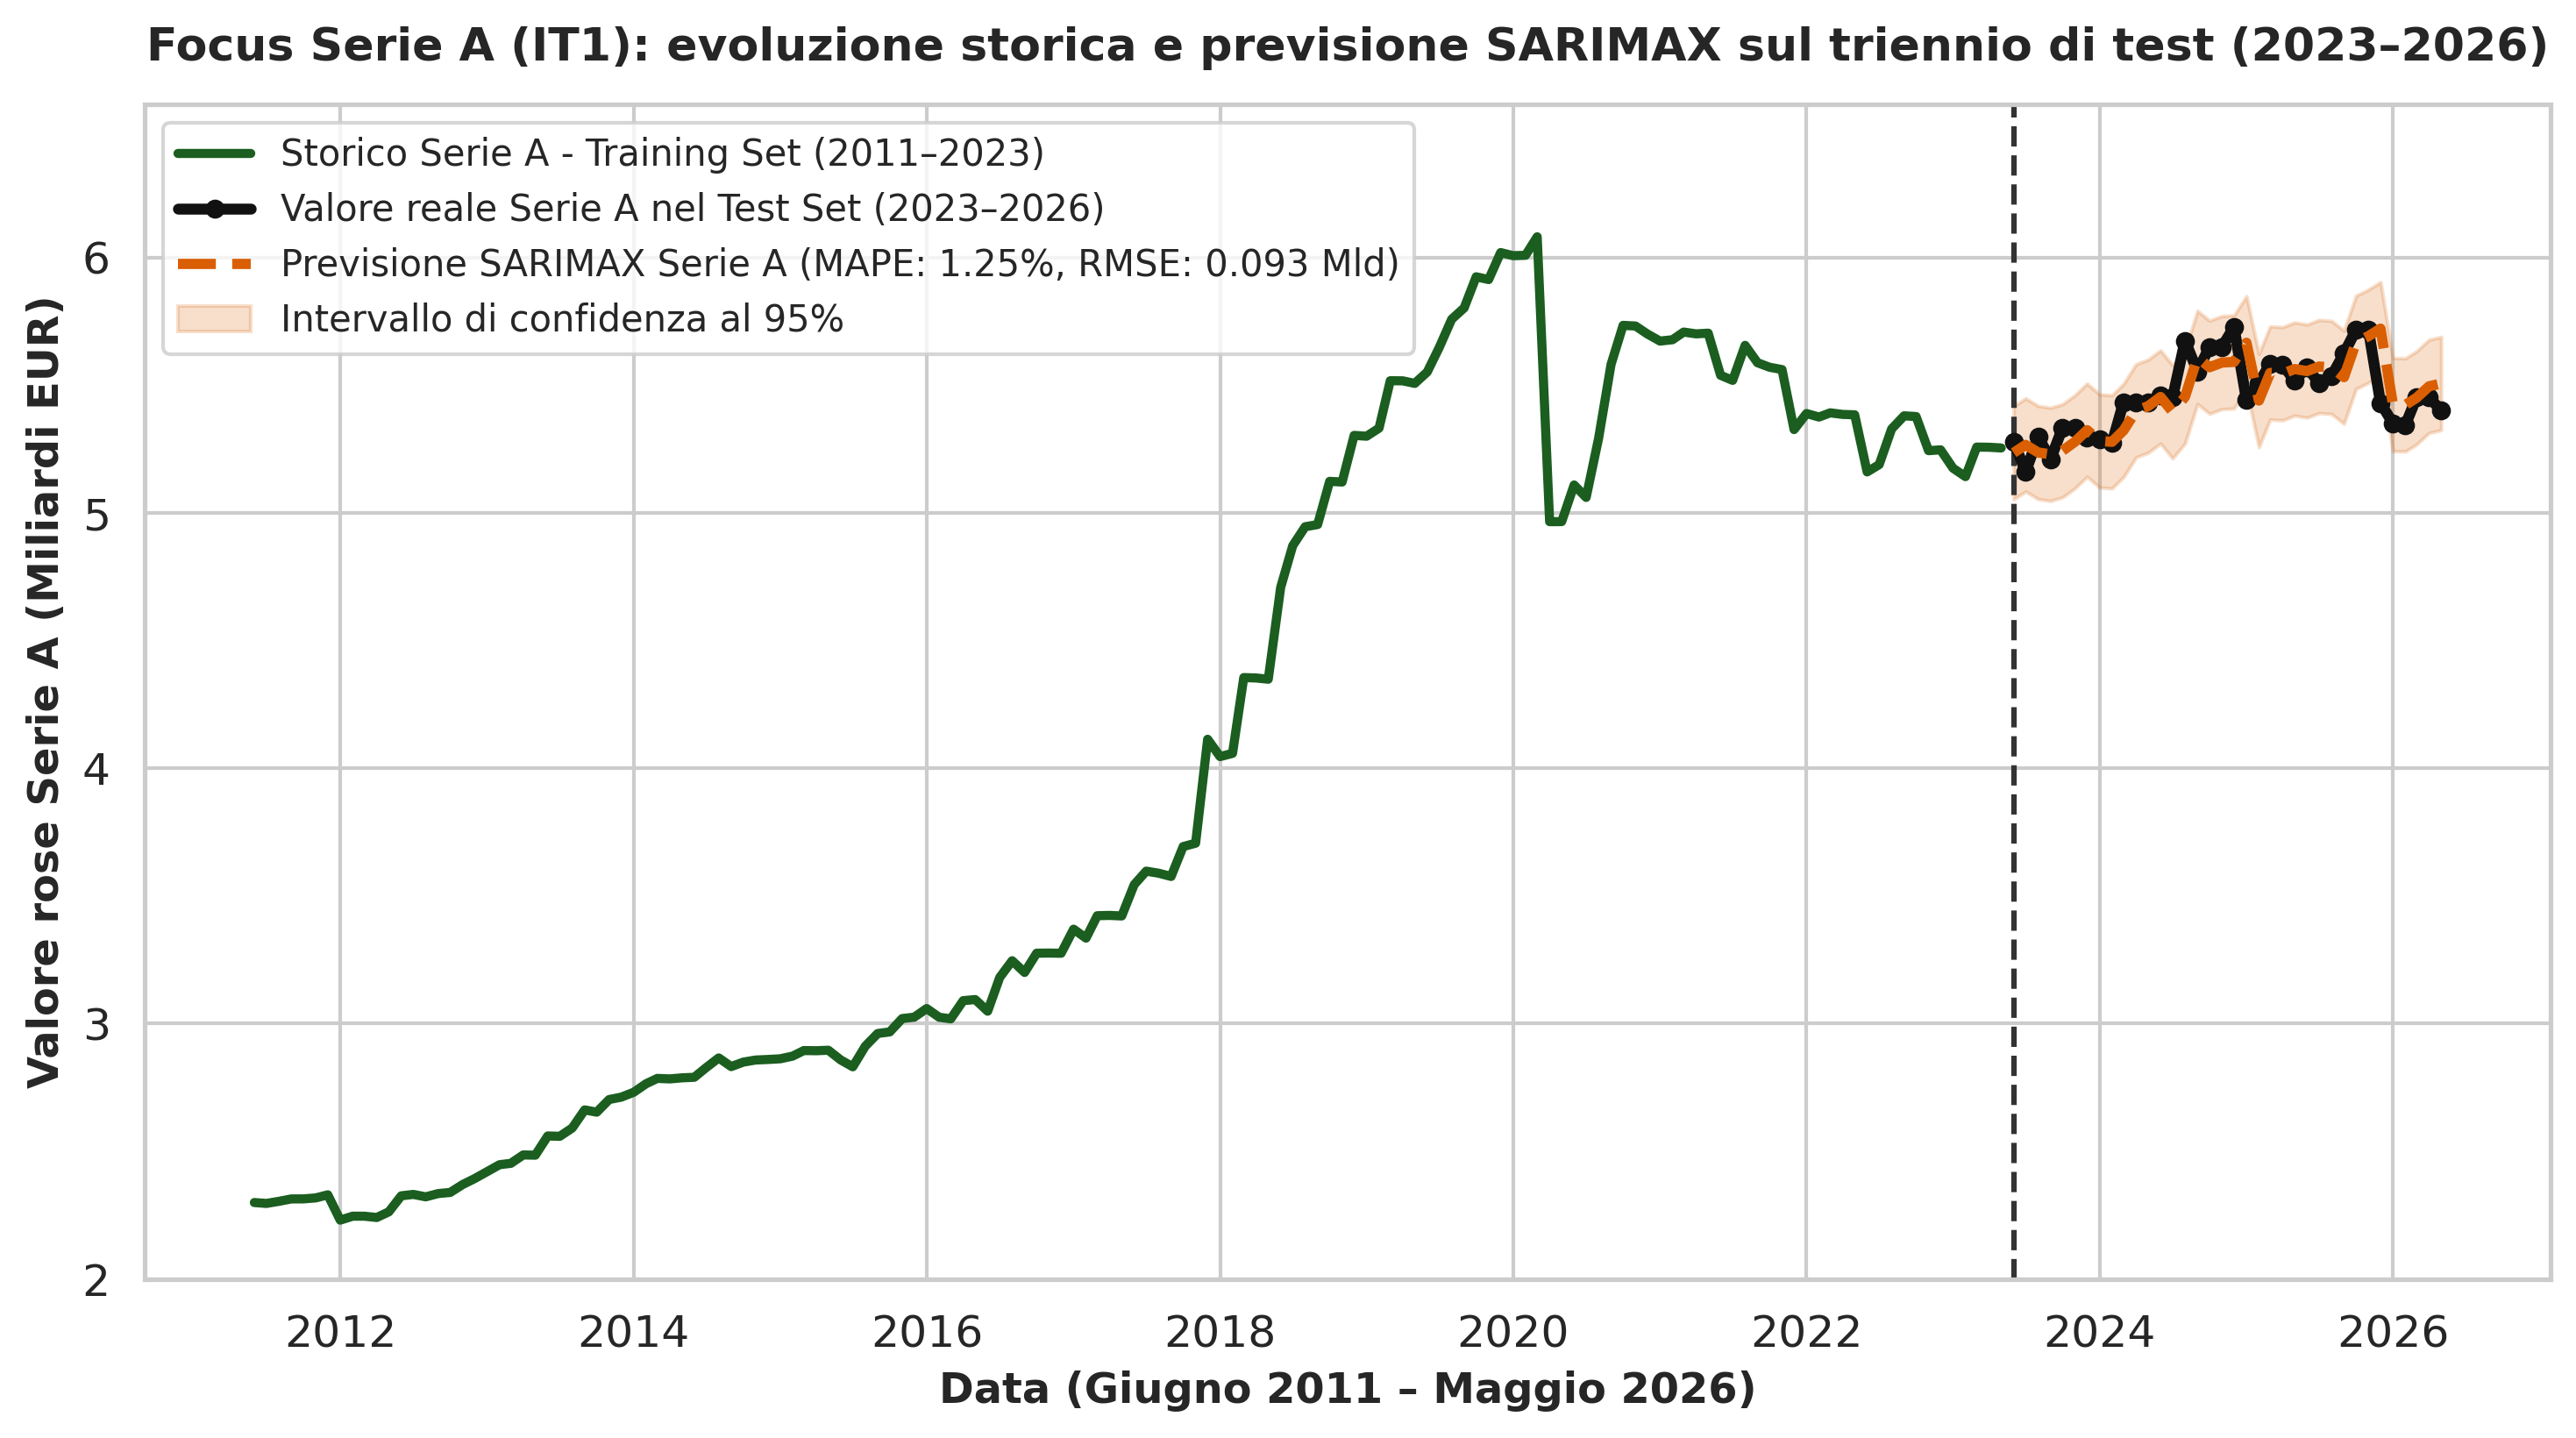
\includegraphics[width=0.95\textwidth]{capitolo9/img/fig21_focus_previsione_serie_a.png}
    \caption{Focus Serie A (\texttt{IT1}): serie storica del valore patrimoniale delle rose e previsione fuori campione del modello SARIMAX nel triennio giugno 2023 -- maggio 2026.}
    \label{fig:focus_serie_a}
\end{figure}

La Figura \ref{fig:focus_serie_a} illustra l'ottima aderenza della previsione SARIMAX (linea tratteggiata arancione) all'andamento effettivo della Serie A lungo i 36 mesi del set di verifica. Mentre la Baseline Naive per il campionato italiano registra un $\mathrm{RMSE}$ di $0,261$ miliardi di euro ($\mathrm{MAE} = 0,219$ miliardi, $\mathrm{MAPE} = 3,96\%$), il modello SARIMAX dedicato alla Serie A riduce l'errore quadratico medio a \textbf{$\mathrm{RMSE} = 0,098$ miliardi di euro} (98 milioni di euro su un patrimonio di oltre 5,4 miliardi), con un errore assoluto medio di \textbf{$\mathrm{MAE} = 0,074$ miliardi} e un errore percentuale medio pari a \textbf{$\mathrm{MAPE} = 1,35\%$}. Il modello riesce a prevedere con precisione sia i picchi autunnali legati alle sessioni estive del 2024 e del 2025 ($5,73$ e $5,72$ miliardi di euro), sia l'assestamento finale a $5,40$ miliardi nel maggio 2026, confermando come la dinamica patrimoniale dei club italiani sia strettamente governata dai volumi di investimento immessi nelle sessioni di calciomercato.

\subsection{Conclusioni della seconda parte e sintesi generale dell'elaborato}

Lo studio condotto in questa seconda parte dell'elaborato ha dimostrato come un patrimonio informativo complesso e relazionale quale il database storico di Transfermarkt possa essere trasformato, mediante una rigorosa pipeline di ingegneria dei dati, in un laboratorio econometrico ad alta precisione per l'analisi delle serie storiche.

Ripercorrendo i risultati principali ottenuti lungo i quattro capitoli dedicati al mercato calcistico europeo, emergono tre conclusioni fondamentali. In primo luogo, sul piano metodologico (Capitolo 6), è stato provato che l'aggregazione ingenua dei listini di valutazione senza la ricostruzione dinamica dell'appartenenza storica dei calciatori ai club tramite presenze e trasferimenti introduce una severa distorsione retrospettiva (sottostimando la Serie A di quasi un miliardo di euro nel biennio 2019--2020), mentre l'integrazione congiunta delle fonti consente di ottenere una serie mensile regolare di 180 osservazioni priva di discontinuità artificiali. In secondo luogo, sul piano economico e strutturale (Capitoli 7 e 8), la decomposizione STL e l'analisi delle variazioni percentuali hanno messo in luce un mercato dominato da un fortissimo trend secolare ($F_T = 0,992$, $+209,7\%$ in quindici anni con una crescente egemonia della Premier League al $39,3\%$ del totale) e scandito da tre rotture di regime: l'accelerazione inflattiva innescata dal trasferimento di Neymar nell'agosto 2017 (che ha quadruplicato il tasso di crescita annuale da $+1,31$ a $+5,46$ miliardi di euro all'anno), il crollo simmetrico del $-18,17\%$ nell'aprile 2020 dovuto alla pandemia da COVID-19 (riassorbito solo dopo 55 mesi nell'ottobre 2024) e il nuovo ciclo espansivo del 2023--2026 che ha spinto il valore medio per calciatore a $11,01$ milioni di euro. In terzo luogo, sul piano predittivo (Capitolo 9), il confronto fuori campione sul triennio 2023--2026 ha certificato la netta superiorità del modello $\mathrm{SARIMAX}(1, 1, 1) \times (1, 0, 1)_{12}$ assistito dalle variabili esogene di spesa del calciomercato, capace di abbattere l'errore percentuale medio fino all'$1,08\%$ sull'aggregato europeo e all'$1,35\%$ sulla Serie A, superando brillantemente i controlli diagnostici di Ljung-Box sui residui.

Considerando unitariamente le due parti che compongono il presente progetto di Data Science — l'analisi supervisionata e non supervisionata sul catalogo musicale di Spotify nella Parte I e l'analisi delle serie storiche sul mercato calcistico di Transfermarkt nella Parte II — il lavoro svolto mette in evidenza un filo conduttore metodologico chiaro: in entrambi i domini applicativi, il successo dei modelli di apprendimento statistico e di previsione non dipende soltanto dalla sofisticazione matematica degli algoritmi impiegati, ma poggia in maniera determinante sulla qualità dell'ingegneria delle feature, sulla comprensione profonda del dominio di business e sulla rigorosa validazione sperimentale dei risultati.


\newpage
\addcontentsline{toc}{section}{\listfigurename}
\listoffigures

\newpage
\addcontentsline{toc}{section}{\listtablename}
\listoftables

\end{document}

